\begin{filecontents*}{\jobname.xmpdata}
  \Title{Your Thesis Title}
  \Author{Matthew Asher Bardin}
  \Keywords{comma, separated, keywords}
  \Date{2023-05-31}
  \Language{en-US}
\end{filecontents*}
%
\documentclass[doublespacing]{lsuthesis}
%% To experiment with using a different document class, such as the ``book''
%% class, comment-out the prior line and uncomment the next line.
%\documentclass[10pt,oneside]{book}

%% Specify additional LaTeX packages you need.
%\usepackage{graphicx}
%\usepackage{amsmath}
%\usepackage{amsthm}
\usepackage{pdfpages}
\usepackage{url}
\DeclareUnicodeCharacter{2212}{-}
 %%%%%%%%%%%%%%%%%%%%%%%%%%%%%%%%%%%%%%%%%%%%%%%%%%%%%%%%%%%%%%%%%%%%%%%%%%%%%%%% 
%%% ~ Arduino Language - Arduino IDE Colors ~                                  %%%
%%%                                                                            %%%
%%% Kyle Rocha-Brownell | 10/2/2017 | No Licence                               %%%
%%% -------------------------------------------------------------------------- %%%
%%%                                                                            %%%
%%% Place this file in your working directory (next to the latex file you're   %%%
%%% working on).  To add it to your project, place:                            %%%
%%%     %%%%%%%%%%%%%%%%%%%%%%%%%%%%%%%%%%%%%%%%%%%%%%%%%%%%%%%%%%%%%%%%%%%%%%%%%%%%%%%% 
%%% ~ Arduino Language - Arduino IDE Colors ~                                  %%%
%%%                                                                            %%%
%%% Kyle Rocha-Brownell | 10/2/2017 | No Licence                               %%%
%%% -------------------------------------------------------------------------- %%%
%%%                                                                            %%%
%%% Place this file in your working directory (next to the latex file you're   %%%
%%% working on).  To add it to your project, place:                            %%%
%%%     %%%%%%%%%%%%%%%%%%%%%%%%%%%%%%%%%%%%%%%%%%%%%%%%%%%%%%%%%%%%%%%%%%%%%%%%%%%%%%%% 
%%% ~ Arduino Language - Arduino IDE Colors ~                                  %%%
%%%                                                                            %%%
%%% Kyle Rocha-Brownell | 10/2/2017 | No Licence                               %%%
%%% -------------------------------------------------------------------------- %%%
%%%                                                                            %%%
%%% Place this file in your working directory (next to the latex file you're   %%%
%%% working on).  To add it to your project, place:                            %%%
%%%    \input{arduinoLanguage.tex}                                             %%%
%%% somewhere before \begin{document} in your latex file.                      %%%
%%%                                                                            %%%
%%% In your document, place your arduino code between:                         %%%
%%%   \begin{lstlisting}[language=Arduino]                                     %%%
%%% and:                                                                       %%%
%%%   \end{lstlisting}                                                         %%%
%%%                                                                            %%%
%%% Or create your own style to add non-built-in functions and variables.      %%%
%%%                                                                            %%%
 %%%%%%%%%%%%%%%%%%%%%%%%%%%%%%%%%%%%%%%%%%%%%%%%%%%%%%%%%%%%%%%%%%%%%%%%%%%%%%%% 

\usepackage{color}
\usepackage{listings}    
\usepackage{courier}

%%% Define Custom IDE Colors %%%
\definecolor{arduinoGreen}    {rgb} {0.17, 0.43, 0.01}
\definecolor{arduinoGrey}     {rgb} {0.47, 0.47, 0.33}
\definecolor{arduinoOrange}   {rgb} {0.8 , 0.4 , 0   }
\definecolor{arduinoBlue}     {rgb} {0.01, 0.61, 0.98}
\definecolor{arduinoDarkBlue} {rgb} {0.0 , 0.2 , 0.5 }

%%% Define Arduino Language %%%
\lstdefinelanguage{Arduino}{
  language=C++, % begin with default C++ settings 
%
%
  %%% Keyword Color Group 1 %%%  (called KEYWORD3 by arduino)
  keywordstyle=\color{arduinoGreen},   
  deletekeywords={  % remove all arduino keywords that might be in c++
                break, case, override, final, continue, default, do, else, for, 
                if, return, goto, switch, throw, try, while, setup, loop, export, 
                not, or, and, xor, include, define, elif, else, error, if, ifdef, 
                ifndef, pragma, warning,
                HIGH, LOW, INPUT, INPUT_PULLUP, OUTPUT, DEC, BIN, HEX, OCT, PI, 
                HALF_PI, TWO_PI, LSBFIRST, MSBFIRST, CHANGE, FALLING, RISING, 
                DEFAULT, EXTERNAL, INTERNAL, INTERNAL1V1, INTERNAL2V56, LED_BUILTIN, 
                LED_BUILTIN_RX, LED_BUILTIN_TX, DIGITAL_MESSAGE, FIRMATA_STRING, 
                ANALOG_MESSAGE, REPORT_DIGITAL, REPORT_ANALOG, SET_PIN_MODE, 
                SYSTEM_RESET, SYSEX_START, auto, int8_t, int16_t, int32_t, int64_t, 
                uint8_t, uint16_t, uint32_t, uint64_t, char16_t, char32_t, operator, 
                enum, delete, bool, boolean, byte, char, const, false, float, double, 
                null, NULL, int, long, new, private, protected, public, short, 
                signed, static, volatile, String, void, true, unsigned, word, array, 
                sizeof, dynamic_cast, typedef, const_cast, struct, static_cast, union, 
                friend, extern, class, reinterpret_cast, register, explicit, inline, 
                _Bool, complex, _Complex, _Imaginary, atomic_bool, atomic_char, 
                atomic_schar, atomic_uchar, atomic_short, atomic_ushort, atomic_int, 
                atomic_uint, atomic_long, atomic_ulong, atomic_llong, atomic_ullong, 
                virtual, PROGMEM,
                Serial, Serial1, Serial2, Serial3, SerialUSB, Keyboard, Mouse,
                abs, acos, asin, atan, atan2, ceil, constrain, cos, degrees, exp, 
                floor, log, map, max, min, radians, random, randomSeed, round, sin, 
                sq, sqrt, tan, pow, bitRead, bitWrite, bitSet, bitClear, bit, 
                highByte, lowByte, analogReference, analogRead, 
                analogReadResolution, analogWrite, analogWriteResolution, 
                attachInterrupt, detachInterrupt, digitalPinToInterrupt, delay, 
                delayMicroseconds, digitalWrite, digitalRead, interrupts, millis, 
                micros, noInterrupts, noTone, pinMode, pulseIn, pulseInLong, shiftIn, 
                shiftOut, tone, yield, Stream, begin, end, peek, read, print, 
                println, available, availableForWrite, flush, setTimeout, find, 
                findUntil, parseInt, parseFloat, readBytes, readBytesUntil, readString, 
                readStringUntil, trim, toUpperCase, toLowerCase, charAt, compareTo, 
                concat, endsWith, startsWith, equals, equalsIgnoreCase, getBytes, 
                indexOf, lastIndexOf, length, replace, setCharAt, substring, 
                toCharArray, toInt, press, release, releaseAll, accept, click, move, 
                isPressed, isAlphaNumeric, isAlpha, isAscii, isWhitespace, isControl, 
                isDigit, isGraph, isLowerCase, isPrintable, isPunct, isSpace, 
                isUpperCase, isHexadecimalDigit, 
                }, 
  morekeywords={   % add arduino structures to group 1
                break, case, override, final, continue, default, do, else, for, 
                if, return, goto, switch, throw, try, while, setup, loop, export, 
                not, or, and, xor, include, define, elif, else, error, if, ifdef, 
                ifndef, pragma, warning,
                }, 
% 
%
  %%% Keyword Color Group 2 %%%  (called LITERAL1 by arduino)
  keywordstyle=[2]\color{arduinoBlue},   
  keywords=[2]{   % add variables and dataTypes as 2nd group  
                HIGH, LOW, INPUT, INPUT_PULLUP, OUTPUT, DEC, BIN, HEX, OCT, PI, 
                HALF_PI, TWO_PI, LSBFIRST, MSBFIRST, CHANGE, FALLING, RISING, 
                DEFAULT, EXTERNAL, INTERNAL, INTERNAL1V1, INTERNAL2V56, LED_BUILTIN, 
                LED_BUILTIN_RX, LED_BUILTIN_TX, DIGITAL_MESSAGE, FIRMATA_STRING, 
                ANALOG_MESSAGE, REPORT_DIGITAL, REPORT_ANALOG, SET_PIN_MODE, 
                SYSTEM_RESET, SYSEX_START, auto, int8_t, int16_t, int32_t, int64_t, 
                uint8_t, uint16_t, uint32_t, uint64_t, char16_t, char32_t, operator, 
                enum, delete, bool, boolean, byte, char, const, false, float, double, 
                null, NULL, int, long, new, private, protected, public, short, 
                signed, static, volatile, String, void, true, unsigned, word, array, 
                sizeof, dynamic_cast, typedef, const_cast, struct, static_cast, union, 
                friend, extern, class, reinterpret_cast, register, explicit, inline, 
                _Bool, complex, _Complex, _Imaginary, atomic_bool, atomic_char, 
                atomic_schar, atomic_uchar, atomic_short, atomic_ushort, atomic_int, 
                atomic_uint, atomic_long, atomic_ulong, atomic_llong, atomic_ullong, 
                virtual, PROGMEM,
                },  
% 
%
  %%% Keyword Color Group 3 %%%  (called KEYWORD1 by arduino)
  keywordstyle=[3]\bfseries\color{arduinoOrange},
  keywords=[3]{  % add built-in functions as a 3rd group
                Serial, Serial1, Serial2, Serial3, SerialBT, airFlow, SerialUSB, Keyboard, Mouse,
                },      
%
%
  %%% Keyword Color Group 4 %%%  (called KEYWORD2 by arduino)
  keywordstyle=[4]\color{arduinoOrange},
  keywords=[4]{  % add more built-in functions as a 4th group
                abs, acos, asin, atan, atan2, ceil, constrain, cos, degrees, exp, 
                floor, log, map, max, min, radians, random, randomSeed, round, sin, 
                sq, sqrt, tan, pow, bitRead, bitWrite, bitSet, bitClear, bit, 
                highByte, lowByte, analogReference, analogRead, 
                analogReadResolution, analogWrite, analogWriteResolution, 
                attachInterrupt, detachInterrupt, digitalPinToInterrupt, delay, 
                delayMicroseconds, digitalWrite, digitalRead, interrupts, millis, 
                micros, noInterrupts, noTone, pinMode, pulseIn, pulseInLong, shiftIn, 
                shiftOut, tone, yield, Stream, begin, end, peek, read, print, 
                println, available, availableForWrite, flush, setTimeout, find, 
                findUntil, parseInt, parseFloat, readBytes, readBytesUntil, readString, 
                readStringUntil, trim, toUpperCase, toLowerCase, charAt, compareTo, 
                concat, endsWith, startsWith, equals, equalsIgnoreCase, getBytes, 
                indexOf, lastIndexOf, length, replace, setCharAt, substring, 
                toCharArray, toInt, press, release, releaseAll, accept, click, move, 
                isPressed, isAlphaNumeric, isAlpha, isAscii, isWhitespace, isControl, 
                isDigit, isGraph, isLowerCase, isPrintable, isPunct, isSpace, 
                isUpperCase, isHexadecimalDigit, Wire, write, beginTransmission, endTransmission
                },      
%
%
  %%% Set Other Colors %%%
  stringstyle=\color{arduinoDarkBlue},    
  commentstyle=\color{arduinoGrey},    
%          
%   
  %%%% Line Numbering %%%%
  numbers=left,                    
  numbersep=5pt,                   
  numberstyle=\color{arduinoGrey},    
  %stepnumber=2,                      % show every 2 line numbers
%
%
  %%%% Code Box Style %%%%
  breaklines=true,                    % wordwrapping
  tabsize=2,         
  basicstyle=\ttfamily  
}
                                             %%%
%%% somewhere before \begin{document} in your latex file.                      %%%
%%%                                                                            %%%
%%% In your document, place your arduino code between:                         %%%
%%%   \begin{lstlisting}[language=Arduino]                                     %%%
%%% and:                                                                       %%%
%%%   \end{lstlisting}                                                         %%%
%%%                                                                            %%%
%%% Or create your own style to add non-built-in functions and variables.      %%%
%%%                                                                            %%%
 %%%%%%%%%%%%%%%%%%%%%%%%%%%%%%%%%%%%%%%%%%%%%%%%%%%%%%%%%%%%%%%%%%%%%%%%%%%%%%%% 

\usepackage{color}
\usepackage{listings}    
\usepackage{courier}

%%% Define Custom IDE Colors %%%
\definecolor{arduinoGreen}    {rgb} {0.17, 0.43, 0.01}
\definecolor{arduinoGrey}     {rgb} {0.47, 0.47, 0.33}
\definecolor{arduinoOrange}   {rgb} {0.8 , 0.4 , 0   }
\definecolor{arduinoBlue}     {rgb} {0.01, 0.61, 0.98}
\definecolor{arduinoDarkBlue} {rgb} {0.0 , 0.2 , 0.5 }

%%% Define Arduino Language %%%
\lstdefinelanguage{Arduino}{
  language=C++, % begin with default C++ settings 
%
%
  %%% Keyword Color Group 1 %%%  (called KEYWORD3 by arduino)
  keywordstyle=\color{arduinoGreen},   
  deletekeywords={  % remove all arduino keywords that might be in c++
                break, case, override, final, continue, default, do, else, for, 
                if, return, goto, switch, throw, try, while, setup, loop, export, 
                not, or, and, xor, include, define, elif, else, error, if, ifdef, 
                ifndef, pragma, warning,
                HIGH, LOW, INPUT, INPUT_PULLUP, OUTPUT, DEC, BIN, HEX, OCT, PI, 
                HALF_PI, TWO_PI, LSBFIRST, MSBFIRST, CHANGE, FALLING, RISING, 
                DEFAULT, EXTERNAL, INTERNAL, INTERNAL1V1, INTERNAL2V56, LED_BUILTIN, 
                LED_BUILTIN_RX, LED_BUILTIN_TX, DIGITAL_MESSAGE, FIRMATA_STRING, 
                ANALOG_MESSAGE, REPORT_DIGITAL, REPORT_ANALOG, SET_PIN_MODE, 
                SYSTEM_RESET, SYSEX_START, auto, int8_t, int16_t, int32_t, int64_t, 
                uint8_t, uint16_t, uint32_t, uint64_t, char16_t, char32_t, operator, 
                enum, delete, bool, boolean, byte, char, const, false, float, double, 
                null, NULL, int, long, new, private, protected, public, short, 
                signed, static, volatile, String, void, true, unsigned, word, array, 
                sizeof, dynamic_cast, typedef, const_cast, struct, static_cast, union, 
                friend, extern, class, reinterpret_cast, register, explicit, inline, 
                _Bool, complex, _Complex, _Imaginary, atomic_bool, atomic_char, 
                atomic_schar, atomic_uchar, atomic_short, atomic_ushort, atomic_int, 
                atomic_uint, atomic_long, atomic_ulong, atomic_llong, atomic_ullong, 
                virtual, PROGMEM,
                Serial, Serial1, Serial2, Serial3, SerialUSB, Keyboard, Mouse,
                abs, acos, asin, atan, atan2, ceil, constrain, cos, degrees, exp, 
                floor, log, map, max, min, radians, random, randomSeed, round, sin, 
                sq, sqrt, tan, pow, bitRead, bitWrite, bitSet, bitClear, bit, 
                highByte, lowByte, analogReference, analogRead, 
                analogReadResolution, analogWrite, analogWriteResolution, 
                attachInterrupt, detachInterrupt, digitalPinToInterrupt, delay, 
                delayMicroseconds, digitalWrite, digitalRead, interrupts, millis, 
                micros, noInterrupts, noTone, pinMode, pulseIn, pulseInLong, shiftIn, 
                shiftOut, tone, yield, Stream, begin, end, peek, read, print, 
                println, available, availableForWrite, flush, setTimeout, find, 
                findUntil, parseInt, parseFloat, readBytes, readBytesUntil, readString, 
                readStringUntil, trim, toUpperCase, toLowerCase, charAt, compareTo, 
                concat, endsWith, startsWith, equals, equalsIgnoreCase, getBytes, 
                indexOf, lastIndexOf, length, replace, setCharAt, substring, 
                toCharArray, toInt, press, release, releaseAll, accept, click, move, 
                isPressed, isAlphaNumeric, isAlpha, isAscii, isWhitespace, isControl, 
                isDigit, isGraph, isLowerCase, isPrintable, isPunct, isSpace, 
                isUpperCase, isHexadecimalDigit, 
                }, 
  morekeywords={   % add arduino structures to group 1
                break, case, override, final, continue, default, do, else, for, 
                if, return, goto, switch, throw, try, while, setup, loop, export, 
                not, or, and, xor, include, define, elif, else, error, if, ifdef, 
                ifndef, pragma, warning,
                }, 
% 
%
  %%% Keyword Color Group 2 %%%  (called LITERAL1 by arduino)
  keywordstyle=[2]\color{arduinoBlue},   
  keywords=[2]{   % add variables and dataTypes as 2nd group  
                HIGH, LOW, INPUT, INPUT_PULLUP, OUTPUT, DEC, BIN, HEX, OCT, PI, 
                HALF_PI, TWO_PI, LSBFIRST, MSBFIRST, CHANGE, FALLING, RISING, 
                DEFAULT, EXTERNAL, INTERNAL, INTERNAL1V1, INTERNAL2V56, LED_BUILTIN, 
                LED_BUILTIN_RX, LED_BUILTIN_TX, DIGITAL_MESSAGE, FIRMATA_STRING, 
                ANALOG_MESSAGE, REPORT_DIGITAL, REPORT_ANALOG, SET_PIN_MODE, 
                SYSTEM_RESET, SYSEX_START, auto, int8_t, int16_t, int32_t, int64_t, 
                uint8_t, uint16_t, uint32_t, uint64_t, char16_t, char32_t, operator, 
                enum, delete, bool, boolean, byte, char, const, false, float, double, 
                null, NULL, int, long, new, private, protected, public, short, 
                signed, static, volatile, String, void, true, unsigned, word, array, 
                sizeof, dynamic_cast, typedef, const_cast, struct, static_cast, union, 
                friend, extern, class, reinterpret_cast, register, explicit, inline, 
                _Bool, complex, _Complex, _Imaginary, atomic_bool, atomic_char, 
                atomic_schar, atomic_uchar, atomic_short, atomic_ushort, atomic_int, 
                atomic_uint, atomic_long, atomic_ulong, atomic_llong, atomic_ullong, 
                virtual, PROGMEM,
                },  
% 
%
  %%% Keyword Color Group 3 %%%  (called KEYWORD1 by arduino)
  keywordstyle=[3]\bfseries\color{arduinoOrange},
  keywords=[3]{  % add built-in functions as a 3rd group
                Serial, Serial1, Serial2, Serial3, SerialBT, airFlow, SerialUSB, Keyboard, Mouse,
                },      
%
%
  %%% Keyword Color Group 4 %%%  (called KEYWORD2 by arduino)
  keywordstyle=[4]\color{arduinoOrange},
  keywords=[4]{  % add more built-in functions as a 4th group
                abs, acos, asin, atan, atan2, ceil, constrain, cos, degrees, exp, 
                floor, log, map, max, min, radians, random, randomSeed, round, sin, 
                sq, sqrt, tan, pow, bitRead, bitWrite, bitSet, bitClear, bit, 
                highByte, lowByte, analogReference, analogRead, 
                analogReadResolution, analogWrite, analogWriteResolution, 
                attachInterrupt, detachInterrupt, digitalPinToInterrupt, delay, 
                delayMicroseconds, digitalWrite, digitalRead, interrupts, millis, 
                micros, noInterrupts, noTone, pinMode, pulseIn, pulseInLong, shiftIn, 
                shiftOut, tone, yield, Stream, begin, end, peek, read, print, 
                println, available, availableForWrite, flush, setTimeout, find, 
                findUntil, parseInt, parseFloat, readBytes, readBytesUntil, readString, 
                readStringUntil, trim, toUpperCase, toLowerCase, charAt, compareTo, 
                concat, endsWith, startsWith, equals, equalsIgnoreCase, getBytes, 
                indexOf, lastIndexOf, length, replace, setCharAt, substring, 
                toCharArray, toInt, press, release, releaseAll, accept, click, move, 
                isPressed, isAlphaNumeric, isAlpha, isAscii, isWhitespace, isControl, 
                isDigit, isGraph, isLowerCase, isPrintable, isPunct, isSpace, 
                isUpperCase, isHexadecimalDigit, Wire, write, beginTransmission, endTransmission
                },      
%
%
  %%% Set Other Colors %%%
  stringstyle=\color{arduinoDarkBlue},    
  commentstyle=\color{arduinoGrey},    
%          
%   
  %%%% Line Numbering %%%%
  numbers=left,                    
  numbersep=5pt,                   
  numberstyle=\color{arduinoGrey},    
  %stepnumber=2,                      % show every 2 line numbers
%
%
  %%%% Code Box Style %%%%
  breaklines=true,                    % wordwrapping
  tabsize=2,         
  basicstyle=\ttfamily  
}
                                             %%%
%%% somewhere before \begin{document} in your latex file.                      %%%
%%%                                                                            %%%
%%% In your document, place your arduino code between:                         %%%
%%%   \begin{lstlisting}[language=Arduino]                                     %%%
%%% and:                                                                       %%%
%%%   \end{lstlisting}                                                         %%%
%%%                                                                            %%%
%%% Or create your own style to add non-built-in functions and variables.      %%%
%%%                                                                            %%%
 %%%%%%%%%%%%%%%%%%%%%%%%%%%%%%%%%%%%%%%%%%%%%%%%%%%%%%%%%%%%%%%%%%%%%%%%%%%%%%%% 

\usepackage{color}
\usepackage{listings}    
\usepackage{courier}

%%% Define Custom IDE Colors %%%
\definecolor{arduinoGreen}    {rgb} {0.17, 0.43, 0.01}
\definecolor{arduinoGrey}     {rgb} {0.47, 0.47, 0.33}
\definecolor{arduinoOrange}   {rgb} {0.8 , 0.4 , 0   }
\definecolor{arduinoBlue}     {rgb} {0.01, 0.61, 0.98}
\definecolor{arduinoDarkBlue} {rgb} {0.0 , 0.2 , 0.5 }

%%% Define Arduino Language %%%
\lstdefinelanguage{Arduino}{
  language=C++, % begin with default C++ settings 
%
%
  %%% Keyword Color Group 1 %%%  (called KEYWORD3 by arduino)
  keywordstyle=\color{arduinoGreen},   
  deletekeywords={  % remove all arduino keywords that might be in c++
                break, case, override, final, continue, default, do, else, for, 
                if, return, goto, switch, throw, try, while, setup, loop, export, 
                not, or, and, xor, include, define, elif, else, error, if, ifdef, 
                ifndef, pragma, warning,
                HIGH, LOW, INPUT, INPUT_PULLUP, OUTPUT, DEC, BIN, HEX, OCT, PI, 
                HALF_PI, TWO_PI, LSBFIRST, MSBFIRST, CHANGE, FALLING, RISING, 
                DEFAULT, EXTERNAL, INTERNAL, INTERNAL1V1, INTERNAL2V56, LED_BUILTIN, 
                LED_BUILTIN_RX, LED_BUILTIN_TX, DIGITAL_MESSAGE, FIRMATA_STRING, 
                ANALOG_MESSAGE, REPORT_DIGITAL, REPORT_ANALOG, SET_PIN_MODE, 
                SYSTEM_RESET, SYSEX_START, auto, int8_t, int16_t, int32_t, int64_t, 
                uint8_t, uint16_t, uint32_t, uint64_t, char16_t, char32_t, operator, 
                enum, delete, bool, boolean, byte, char, const, false, float, double, 
                null, NULL, int, long, new, private, protected, public, short, 
                signed, static, volatile, String, void, true, unsigned, word, array, 
                sizeof, dynamic_cast, typedef, const_cast, struct, static_cast, union, 
                friend, extern, class, reinterpret_cast, register, explicit, inline, 
                _Bool, complex, _Complex, _Imaginary, atomic_bool, atomic_char, 
                atomic_schar, atomic_uchar, atomic_short, atomic_ushort, atomic_int, 
                atomic_uint, atomic_long, atomic_ulong, atomic_llong, atomic_ullong, 
                virtual, PROGMEM,
                Serial, Serial1, Serial2, Serial3, SerialUSB, Keyboard, Mouse,
                abs, acos, asin, atan, atan2, ceil, constrain, cos, degrees, exp, 
                floor, log, map, max, min, radians, random, randomSeed, round, sin, 
                sq, sqrt, tan, pow, bitRead, bitWrite, bitSet, bitClear, bit, 
                highByte, lowByte, analogReference, analogRead, 
                analogReadResolution, analogWrite, analogWriteResolution, 
                attachInterrupt, detachInterrupt, digitalPinToInterrupt, delay, 
                delayMicroseconds, digitalWrite, digitalRead, interrupts, millis, 
                micros, noInterrupts, noTone, pinMode, pulseIn, pulseInLong, shiftIn, 
                shiftOut, tone, yield, Stream, begin, end, peek, read, print, 
                println, available, availableForWrite, flush, setTimeout, find, 
                findUntil, parseInt, parseFloat, readBytes, readBytesUntil, readString, 
                readStringUntil, trim, toUpperCase, toLowerCase, charAt, compareTo, 
                concat, endsWith, startsWith, equals, equalsIgnoreCase, getBytes, 
                indexOf, lastIndexOf, length, replace, setCharAt, substring, 
                toCharArray, toInt, press, release, releaseAll, accept, click, move, 
                isPressed, isAlphaNumeric, isAlpha, isAscii, isWhitespace, isControl, 
                isDigit, isGraph, isLowerCase, isPrintable, isPunct, isSpace, 
                isUpperCase, isHexadecimalDigit, 
                }, 
  morekeywords={   % add arduino structures to group 1
                break, case, override, final, continue, default, do, else, for, 
                if, return, goto, switch, throw, try, while, setup, loop, export, 
                not, or, and, xor, include, define, elif, else, error, if, ifdef, 
                ifndef, pragma, warning,
                }, 
% 
%
  %%% Keyword Color Group 2 %%%  (called LITERAL1 by arduino)
  keywordstyle=[2]\color{arduinoBlue},   
  keywords=[2]{   % add variables and dataTypes as 2nd group  
                HIGH, LOW, INPUT, INPUT_PULLUP, OUTPUT, DEC, BIN, HEX, OCT, PI, 
                HALF_PI, TWO_PI, LSBFIRST, MSBFIRST, CHANGE, FALLING, RISING, 
                DEFAULT, EXTERNAL, INTERNAL, INTERNAL1V1, INTERNAL2V56, LED_BUILTIN, 
                LED_BUILTIN_RX, LED_BUILTIN_TX, DIGITAL_MESSAGE, FIRMATA_STRING, 
                ANALOG_MESSAGE, REPORT_DIGITAL, REPORT_ANALOG, SET_PIN_MODE, 
                SYSTEM_RESET, SYSEX_START, auto, int8_t, int16_t, int32_t, int64_t, 
                uint8_t, uint16_t, uint32_t, uint64_t, char16_t, char32_t, operator, 
                enum, delete, bool, boolean, byte, char, const, false, float, double, 
                null, NULL, int, long, new, private, protected, public, short, 
                signed, static, volatile, String, void, true, unsigned, word, array, 
                sizeof, dynamic_cast, typedef, const_cast, struct, static_cast, union, 
                friend, extern, class, reinterpret_cast, register, explicit, inline, 
                _Bool, complex, _Complex, _Imaginary, atomic_bool, atomic_char, 
                atomic_schar, atomic_uchar, atomic_short, atomic_ushort, atomic_int, 
                atomic_uint, atomic_long, atomic_ulong, atomic_llong, atomic_ullong, 
                virtual, PROGMEM,
                },  
% 
%
  %%% Keyword Color Group 3 %%%  (called KEYWORD1 by arduino)
  keywordstyle=[3]\bfseries\color{arduinoOrange},
  keywords=[3]{  % add built-in functions as a 3rd group
                Serial, Serial1, Serial2, Serial3, SerialBT, airFlow, SerialUSB, Keyboard, Mouse,
                },      
%
%
  %%% Keyword Color Group 4 %%%  (called KEYWORD2 by arduino)
  keywordstyle=[4]\color{arduinoOrange},
  keywords=[4]{  % add more built-in functions as a 4th group
                abs, acos, asin, atan, atan2, ceil, constrain, cos, degrees, exp, 
                floor, log, map, max, min, radians, random, randomSeed, round, sin, 
                sq, sqrt, tan, pow, bitRead, bitWrite, bitSet, bitClear, bit, 
                highByte, lowByte, analogReference, analogRead, 
                analogReadResolution, analogWrite, analogWriteResolution, 
                attachInterrupt, detachInterrupt, digitalPinToInterrupt, delay, 
                delayMicroseconds, digitalWrite, digitalRead, interrupts, millis, 
                micros, noInterrupts, noTone, pinMode, pulseIn, pulseInLong, shiftIn, 
                shiftOut, tone, yield, Stream, begin, end, peek, read, print, 
                println, available, availableForWrite, flush, setTimeout, find, 
                findUntil, parseInt, parseFloat, readBytes, readBytesUntil, readString, 
                readStringUntil, trim, toUpperCase, toLowerCase, charAt, compareTo, 
                concat, endsWith, startsWith, equals, equalsIgnoreCase, getBytes, 
                indexOf, lastIndexOf, length, replace, setCharAt, substring, 
                toCharArray, toInt, press, release, releaseAll, accept, click, move, 
                isPressed, isAlphaNumeric, isAlpha, isAscii, isWhitespace, isControl, 
                isDigit, isGraph, isLowerCase, isPrintable, isPunct, isSpace, 
                isUpperCase, isHexadecimalDigit, Wire, write, beginTransmission, endTransmission
                },      
%
%
  %%% Set Other Colors %%%
  stringstyle=\color{arduinoDarkBlue},    
  commentstyle=\color{arduinoGrey},    
%          
%   
  %%%% Line Numbering %%%%
  numbers=left,                    
  numbersep=5pt,                   
  numberstyle=\color{arduinoGrey},    
  %stepnumber=2,                      % show every 2 line numbers
%
%
  %%%% Code Box Style %%%%
  breaklines=true,                    % wordwrapping
  tabsize=2,         
  basicstyle=\ttfamily  
}
  
%Define the listing package
\usepackage{listings} %code highlighter
\usepackage{color} %use color
\definecolor{mygreen}{rgb}{0,0.6,0}
\definecolor{mygray}{rgb}{0.5,0.5,0.5}
\definecolor{mymauve}{rgb}{0.58,0,0.82}
 
%Customize a bit the look
\lstset{ %
backgroundcolor=\color{white}, % choose the background color; you must add \usepackage{color} or \usepackage{xcolor}
basicstyle=\footnotesize, % the size of the fonts that are used for the code
breakatwhitespace=false, % sets if automatic breaks should only happen at whitespace
breaklines=true, % sets automatic line breaking
captionpos=b, % sets the caption-position to bottom
commentstyle=\color{mygreen}, % comment style
deletekeywords={...}, % if you want to delete keywords from the given language
escapeinside={\%*}{*)}, % if you want to add LaTeX within your code
extendedchars=true, % lets you use non-ASCII characters; for 8-bits encodings only, does not work with UTF-8
frame=single, % adds a frame around the code
keepspaces=true, % keeps spaces in text, useful for keeping indentation of code (possibly needs columns=flexible)
keywordstyle=\color{blue}, % keyword style
% language=Octave, % the language of the code
morekeywords={*,...}, % if you want to add more keywords to the set
numbers=left, % where to put the line-numbers; possible values are (none, left, right)
numbersep=5pt, % how far the line-numbers are from the code
numberstyle=\tiny\color{mygray}, % the style that is used for the line-numbers
rulecolor=\color{black}, % if not set, the frame-color may be changed on line-breaks within not-black text (e.g. comments (green here))
showspaces=false, % show spaces everywhere adding particular underscores; it overrides 'showstringspaces'
showstringspaces=false, % underline spaces within strings only
showtabs=false, % show tabs within strings adding particular underscores
stepnumber=1, % the step between two line-numbers. If it's 1, each line will be numbered
stringstyle=\color{mymauve}, % string literal style
tabsize=2, % sets default tabsize to 2 spaces
title=\lstname % show the filename of files included with \lstinputlisting; also try caption instead of title
}
%END of listing package%
 
\definecolor{darkgray}{rgb}{.4,.4,.4}
\definecolor{purple}{rgb}{0.65, 0.12, 0.82}
 
%define Javascript language
\lstdefinelanguage{JavaScript}{
keywords={typeof, new, true, false, catch, function, return, null, catch, switch, var, if, in, while, do, else, case, let, for,break},
keywordstyle=\color{blue}\bfseries,
ndkeywords={class, export, boolean, throw, implements, import, this},
ndkeywordstyle=\color{darkgray}\bfseries,
identifierstyle=\color{black},
sensitive=false,
comment=[l]{//},
morecomment=[s]{/*}{*/},
commentstyle=\color{purple}\ttfamily,
stringstyle=\color{red}\ttfamily,
morestring=[b]',
morestring=[b]"
}
 
\lstset{
language=JavaScript,
extendedchars=true,
basicstyle=\footnotesize\ttfamily,
showstringspaces=false,
showspaces=false,
numbers=left,
numberstyle=\footnotesize,
numbersep=9pt,
tabsize=2,
breaklines=true,
showtabs=false,
captionpos=b
}

\usepackage{lsutitle}
\title{Cyberinet: INTEGRATED SEMI-MODULAR SENSORS FOR THE COMPUTER-AUGMENTED CLARINET}
\thesistype{Dissertation}
\department{The School of Music}
\soughtdegree{Doctor of Philosophy}
\author{Matthew Asher Bardin}
\degrees{B.M., Stetson University, 2017\\
  M.M., The Boston Conservatory at Berklee, 2019}
\graduationdate{August 2023}


\begin{document}

%% The command ``\frontmatter'' switches to lowercase roman page numbers and
%% unnumbered chapter headings without the word ``Chapter''.
\frontmatter

\maketitle

%%%%%%%%%%%%%%%%%%%%%%%%%%%%%%%%%%%%%%%%%%%%%%%%%%%%%%%%%%%%%%%%%%%%%%%%%%%%%%
%%%%%%%%%%%%%%%%%%%%%%%%%%%%%%%%%%%%%%%%%%%%%%%%%%%%%%%%%%%%%%%%%%%%%%%%%%%%%%
%%%%%%%%%%%%%%%%%%%%%%%%%%%%%%%%%%%%%%%%%%%%%%%%%%%%%%%%%%%%%%%%%%%%%%%%%%%%%%
%%%%%%%%%%%%%%%%%%%%%%%%%%%%%%%%%%%%%%%%%%%%%%%%%%%%%%%%%%%%%%%%%%%%%%%%%%%%%%
%%%%%%%%%%%%%%%%%%%%%%%%%%%%%%%%%%%%%%%%%%%%%%%%%%%%%%%%%%%%%%%%%%%%%%%%%%%%%%
%% The following ``Copyright'' page is optional. You have inherent copyright
%% on anything you create, even if you choose not to include a copyright
%% notice. But if you choose to also formally register your copyright with
%% the Library of Congress, then a centered copyright notice should follow
%% the title page.
\begin{centeredpage}
\copyright\ 2023\\
Matthew Asher Bardin
\end{centeredpage}  
% Be sure to do this when revising (because $$), before submission to the library.
%%%%%%%%%%%%%%%%%%%%%%%%%%%%%%%%%%%%%%%%%%%%%%%%%%%%%%%%%%%%%%%%%%%%%%%%%%%%%%
%%%%%%%%%%%%%%%%%%%%%%%%%%%%%%%%%%%%%%%%%%%%%%%%%%%%%%%%%%%%%%%%%%%%%%%%%%%%%%
%%%%%%%%%%%%%%%%%%%%%%%%%%%%%%%%%%%%%%%%%%%%%%%%%%%%%%%%%%%%%%%%%%%%%%%%%%%%%%
%%%%%%%%%%%%%%%%%%%%%%%%%%%%%%%%%%%%%%%%%%%%%%%%%%%%%%%%%%%%%%%%%%%%%%%%%%%%%%
%%%%%%%%%%%%%%%%%%%%%%%%%%%%%%%%%%%%%%%%%%%%%%%%%%%%%%%%%%%%%%%%%%%%%%%%%%%%%%

\begin{centeredpage}
\epigraph{\textit{Everything you do is music, and everywhere is the best seat.}}{John Cage}
\end{centeredpage}


\chapter{Acknowledgments}

First, I would like to thank my family. Without their continued support, I would not have been able to make it into graduate school, let alone be finish my dissertation project. Thank you from the bottom of my heart Mom, Dad, Michael, Melanie, and the rest of the extended family. 

I would also like to thank my various professors and mentors that I have had the pleasure of working with over the past decade. From building a general approach to music and technology in my undergraduate studies, to finding my passion while finishing my Master’s degree in Boston, to the guidance I received on this project; the advice I have received from these people has helped me to not only build a strong knowledge base, but achieve the confidence to present my work and my art to the world. I wish I had the time to mention everyone here individually, but I am incredibly grateful to each of my teachers I have had along this journey.

Thanks are also due to my students and other teachers at the Denham Springs High School STEM \& Robotics Center. While working on this project it was refreshing to step away and focus on making creative projects that explore various technology. After teaching there for the past three years, the thought of leaving is bittersweet, but I look forward to following along to see the continued growth of the students and program in future years.

Lastly, I would like to thank my cat, Bean. Regardless of whether she was laying directly on top of the paper I needed to cite; she always made a spot on my desk to join me while I was writing. When in doubt, I would always defer to her expert opinion on any matters related to ear-scratches, pets, and wet food. Bean was more opinionated on these matters than the likes of 3D printing, Max programming, or gesture visualizing. Regardless, I have no doubt these were among the most useful comments I received during the writing process. Thank you, Bean. I could not have finished this project without you.

\vspace{25mm}
\begin{center}
    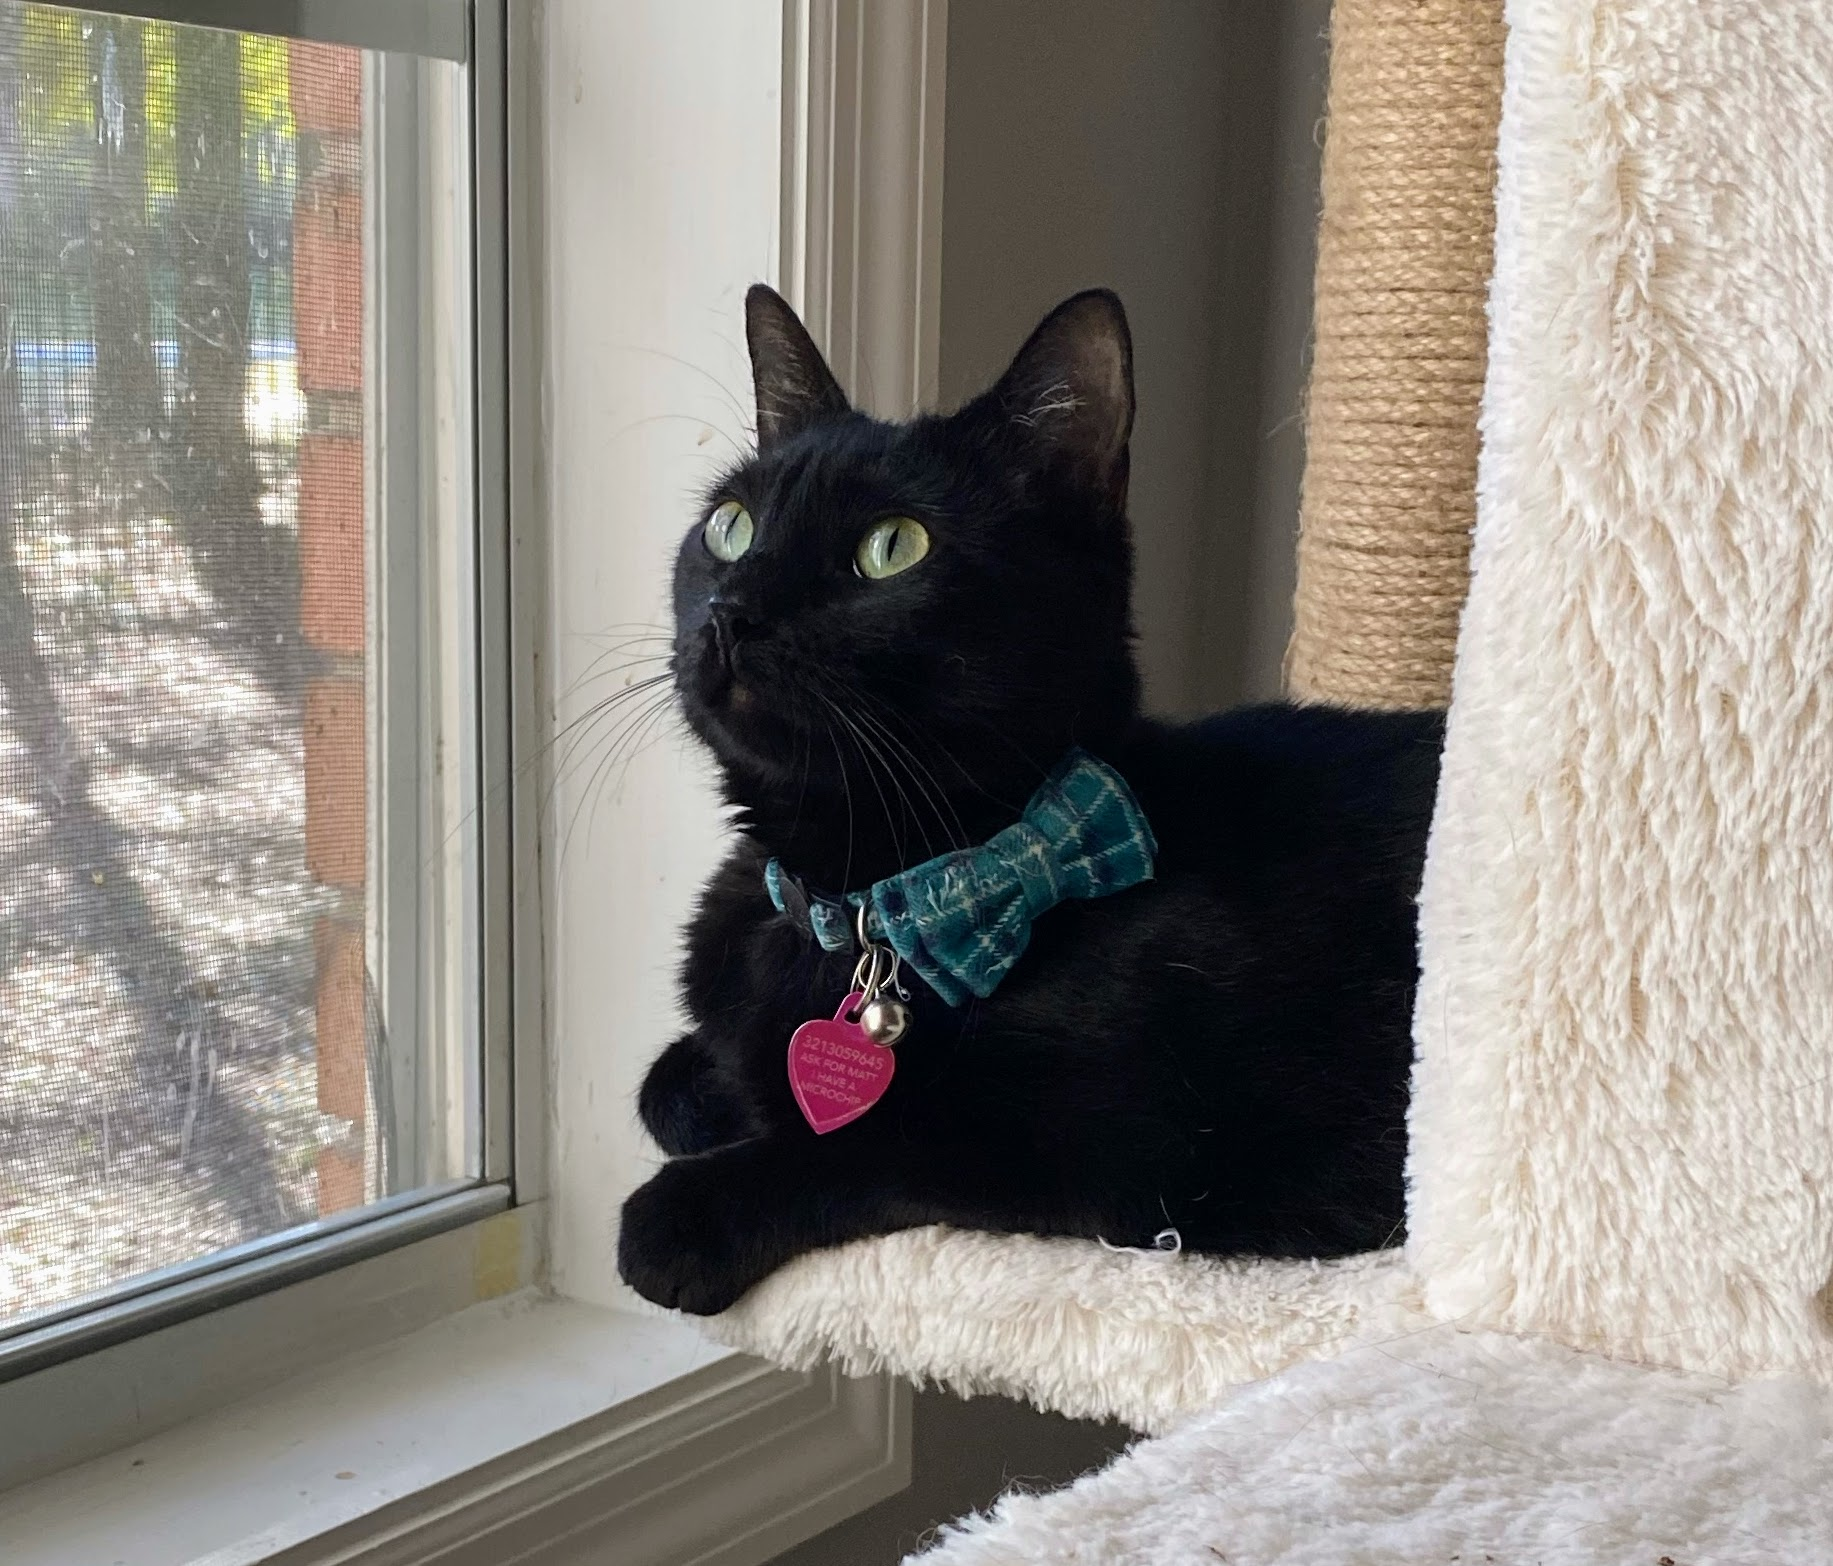
\includegraphics[scale=0.2]{bean.jpeg}
\end{center}

\tableofcontents

 \listoffigures
 \listoftables

\chapter{Abstract}

% The ``abstract'' is required and is limited to 350 words. % this version 344 words.

Augmented instruments have been around in some form for almost as long as instruments, but have had a relatively recent explosion in presence and capabilities due to the progression of technology through the 20th and 21st centuries. One potential use of augmented instruments is to control audio processing on a computer utilizing Max or other software environments. By being able to control the music natural expressive means, the performer and composer are able to experiment with a variety of ways to make sound. A performer is able to hear their sounds and adjust their playing in order to change them in real time, or the sounds are able to react to a performer's movements automatically. creation of future music. One new instrument that works to combine these two ideas is the Cyberinet.

The goal of this project is to provide a method of computer-enhanced performance to the solo Clarinetist with minimal interference to their normal performance practice. A performer utilizing the Cyberinet is able to seamlessly switch between a traditional performance setting and an augmented one. Towards this, the Cyberinet is a hardware replacement for a portion of a Clarinet containing a variety of sensors embedded within the unit. These sensors collect various real time data motion data of the performer and air flow within the instrument. Additional sensors can be connected to the Cyberinet to further expand its capabilities, which allows for the unit to become customizable based on various performance needs. The collected data is then transferred to a computer via Bluetooth connectivity in order to use the data in any number of potential electroacoustic performance settings. 

In order to explore these new relationships, in addition to the instrument itself, a collection of Max objects designed from the ground up to utilize the Cyberinet’s data in musical contexts has been developed. These Max objects were utilized in the performance the first four compositions for the Cyberinet in the spring of 2023.

\mainmatter
\chapter{Defining the Cyberinet} \label{ch:1}

The idea of augmenting an instrument has been around for almost as long as instruments themselves. In the modern sense, an augmented instrument can be defined as any acoustic instrument that has had an increase in functionality due to additional, usually electronic (in recent years), additions to the instrument\cite{miranda_Wanderley_instrumentControl_2006}. While descriptive, this definition leave room for interpretation in exactly how or why the instrument is augmented. This leads to a large variety in terms of what form potential augmentations can take; some of which will be naturally more accessible and adaptable than others. Some of the more common less-desirable traits present in augmented instruments include: requiring permanent alterations to the performer's instrument\footnote{If removable, the setup process is cumbersome or time consuming}, high price, and the act of performing with the augmentation proves difficult to learn, or highly contrasting to the performer's training. 

The Cyberinet is a new augmented instrument indented to address all of these concerns by easily allowing a Clarinettist to not only control audio/visual processing within the Max environment, but is also adaptable with a variety of sensors in order to create a custom setup unique to each user and performance setting.

To qualify as an augmented instrument and not a derivative new instrument, it is important that the augmented instrument retain enough of the original characteristics of the acoustic base\cite{miranda_Wanderley_instrumentControl_2006}. For example, an electric guitar can still functions as a guitar when not utilizing the amplification, or that a trombone still acts like a trombone regardless of when a mute is inserted. Without the context of a base instrument, an augmented instrument is no longer augmented, simply a new instrument. In order to address this, the Cyberinet functions as a digital enhancement to the Clarinet. The barrel of the horn is replaced with the Cyberinet unit, which collects a variety of positional and airflow data for use in digital processing without impeding the traditional performance practice of the instrument. Without the base Clarinet, loses the majority of its functionality.

\begin{figure}
    \centering
    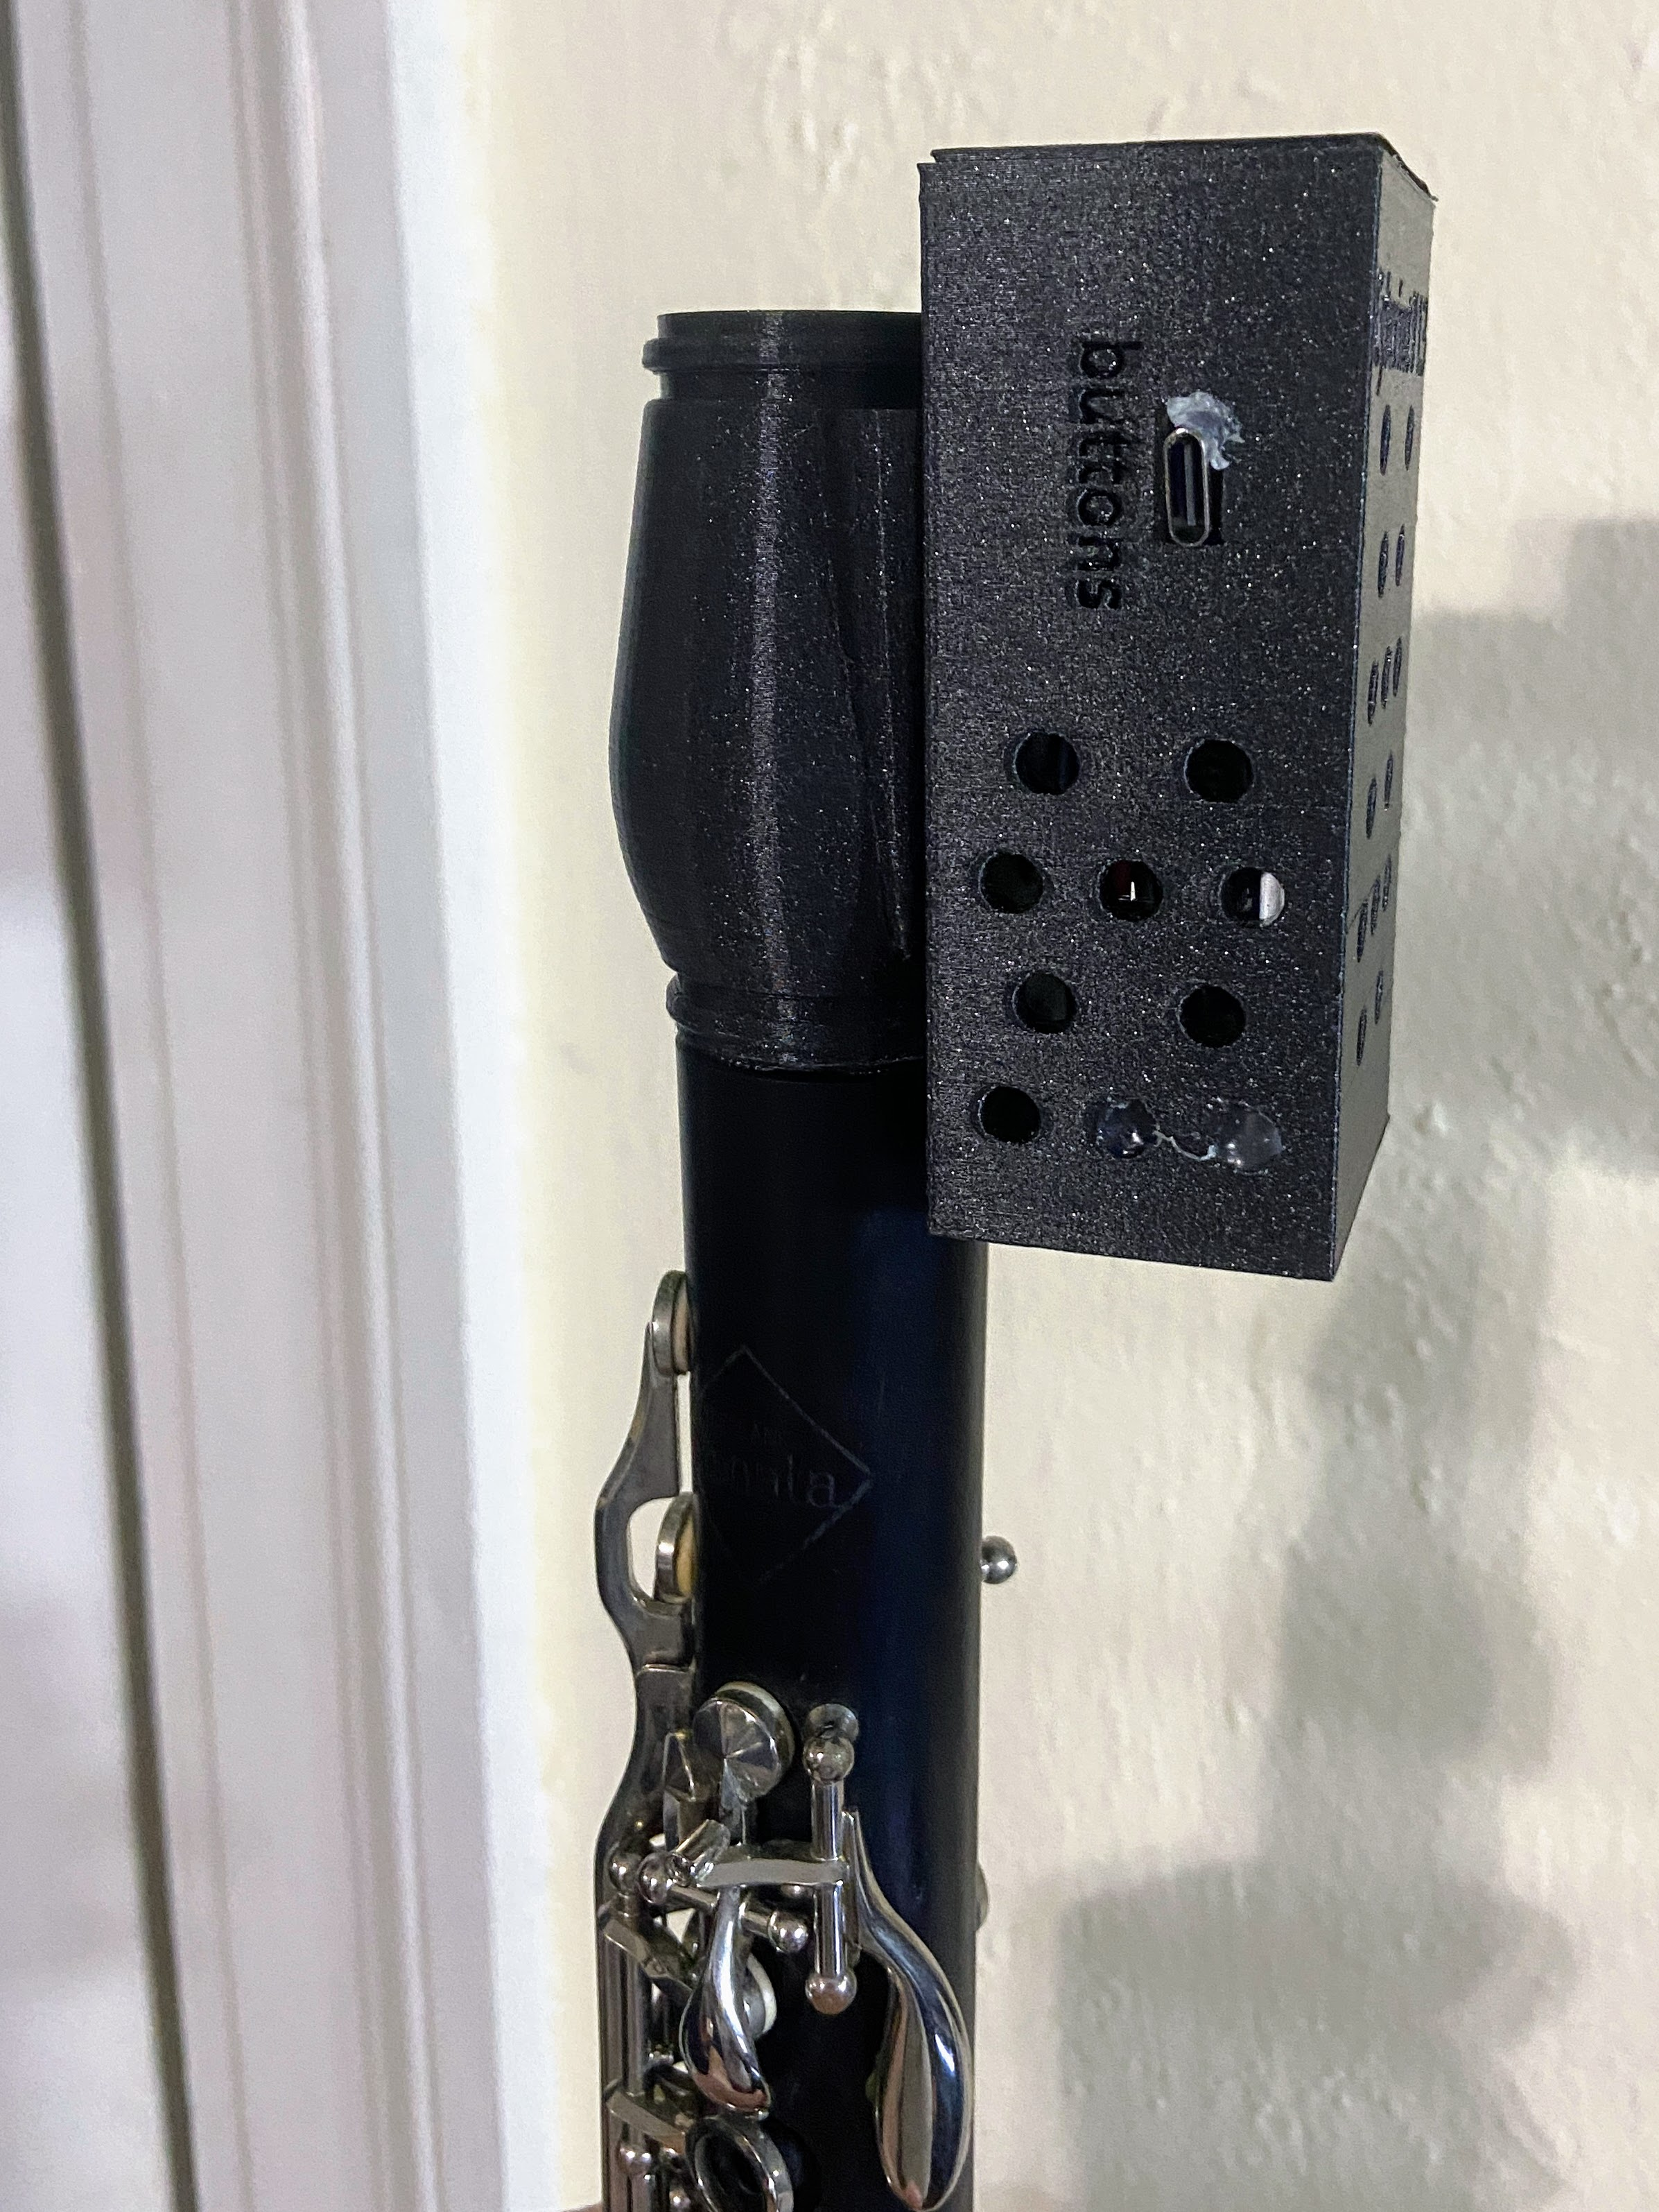
\includegraphics[scale=0.1]{diagrams/IMG_2212.JPG}
    \caption{Cyberinet main unit on a Clarinet. (without mouthpiece)}
    \label{fig:MainUnit}
\end{figure}

The data utilized by the main unit of the Cyberinet is collected through multiple I2C sensors and wirelessly transmitted to a computer in order to control digital signal processing using the Max software. This allows for the performer to respond to the state of the processing by changing how they are performing in real time. The Cyberinet can be used to passively collect data for analysis, or with active use of gestures in order to achieve specific a sound or effect.

By being easily removable, non-invasive, and utilizing wireless communications, the Cyberinet addresses many of the aforementioned concerns with augmented instruments. In terms of cost, the Cyberinet is completely open-source and costs approximately \$120 USD to produce\footnote{This value is the total cost of all sensors, PCB's, and other materials. The cost of a 3D printer is not included in this total.}. This, combined with a free collection of Max objects designed to interface with the Cyberinet's sensors allow for a wider audience to easily implement the augmentation and create new sounds.

\section{Augmented Instruments \& Music}

% define an augmented instrument, give at least two examples. Indicate what is good and what could be improved.

Above anything else, the Cyberinet is an augmented instrument. To better understand exactly what this constitutes, and explore the Cyberinet's augmentations, a better understanding of these inventions is required. Going back several hundred years until the early 21st century, completely mechanical, electronic, and digital augmentations have all been utilized in musical performance. While mechanical and electric augmentations are still commonplace in the 21st century, a majority of modern instrument augmentations are digital in nature, or offer a combination of these three categories.

\subsection{Mechanical Augmentations}

\subsubsection{Brass Mutes}
In many contexts, the idea of augmenting instruments is viewed as a relatively new practice. While there has been an increase in the number of augmented instruments over the past century especially those with electronic and digital augmentations. The concept of improving the capabilities of instruments proceeds the electrical manipulations by centuries. These augmentations usually involve the addition or refinement of the various physical attributes of the instrument.

To clarify this viewpoint, four historical examples of augmentations will be discussed to show their variety. The first is the development of brass mutes. By itself, a brass mute serves as an entirely mechanical and removable augmentation for the instrument it was designed for. A brass player utilizing a mute has a greater range of timbral options when compared to a performer not utilizing a mute. While not the first known instance of a mute being used in modern music, the score to Montiverdi's 1509 opera \textit{Orfeo} opens with this distinct timbre in the trombones, and is well known in Western music history.

\begin{figure}
    \centering
    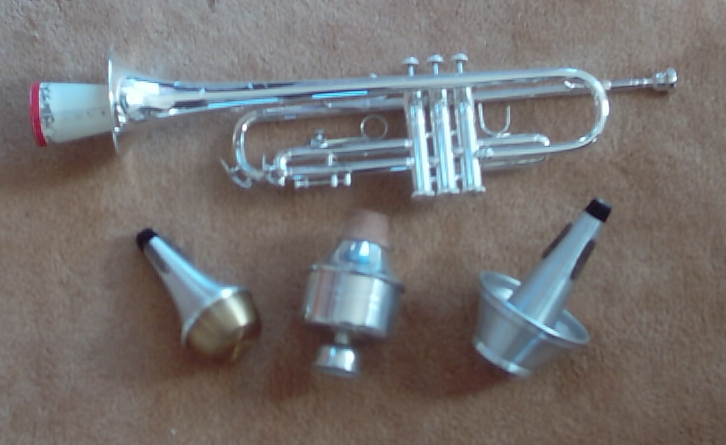
\includegraphics[scale=0.35]{diagrams/TrumpetMutes.jpg}
    \caption{A variety of trumpet mutes, courtesy of Wikimedia Commons.} %wikimedia commons. No permissions needed to use.
    \label{fig:tptmutes}
\end{figure}

Modern versions of brass mutes have been made for every common-place brass instrument\footnote{By common-place I am referring to those used in Western orchestras and bands. These include trumpets, horns, euphoniums, trombones, and tubas.}, and many varieties of mutes have been created to allow for a greater variety of timbre possibilities in both performance and orchestration settings. While mutes will vary slightly based on the instrument and mute design, they all generally work by achieving one goal: absorbing/shifting a portion of the instrument's produced sound waves, filtering the sound, and changing the timbre. Some mutes such as cup and bucket mutes serve to block the sound waves in the air. Harmon mutes create a resonating cone to change the harmonic make up of the sound\cite{brassMutes1982}. Practice mutes serve to minimize the vibration of the bell before the energy can be converted into sound waves. The physicality of the mutes will also block a portion of the air moving through the instrument which both alters how the performer must play their instrument, as well as further altering the sound\cite{brassMutes1982}.

The specific acoustic properties of each brass mute are outside the scope of this document. However, the ability for a user to easily implement changes to their sound by altering the instrument in some way, thus augmenting their timberal range, is the core concept that makes a brass mute fit into the realm of augmented instruments. In many cases, brass instrument performers will own a variety of different mutes in order to further increase their range of timbres in a musical setting.

\subsubsection{Prepared Piano}

Following a similar logic as brass mutes, a prepared piano is an augmentation for a traditional piano. The creation of the prepared piano is often attributed to John Cage in his 1938-40 composition \textit{Bacchanale}, although earlier instances of placing items into the piano strings have been recorded\cite{ppHist}. While more complex and involved than a brass mute, the same concepts apply to the prepared piano. A performer is able to augment the timbral capabilities of the original instrument, the augmentation can be reversed, and the instrument still retains its identity as a piano while prepared. Because of how long it takes to properly augment a piano however, it is less flexible in a performance setting than other augmented instruments\cite{ppArticle}. 

\begin{figure}
    \centering
    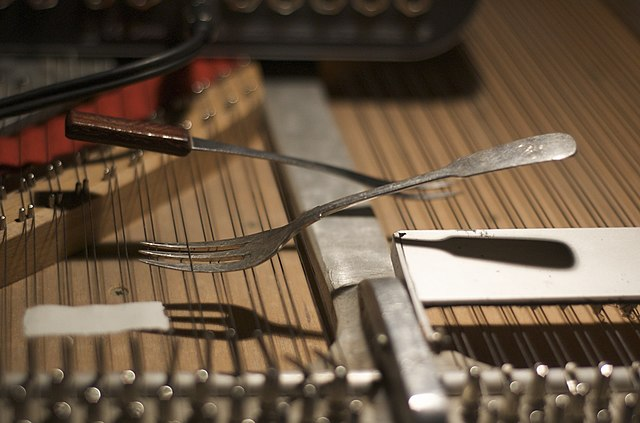
\includegraphics[scale=0.5]{diagrams/Prepared_piano_board_Neumann.jpg}
    \caption{An example of a prepared piano, courtesy of Wikimedia Commons.} % wmC. no attribution needed
    \label{fig:pp}
\end{figure}

The process of preparing a piano is a relatively simple one, although usually time consuming\cite{ppVideo}. The most common of preparations involve placing small objects of varying materials wedged in between the strings for certain notes\cite{ppArticle}. Many composers will include a legend indication how to properly prepare the piano in the materials for a performance. These instructions usually include the specific strings, the item/material to utilize, and where/how to place it along the length of the string. Table \ref{fig:siPrep} recreates a small portion of preparation instructions made by John Cage for his work \textit{Sonatas and Interludes} (1946-48). In the case of Cage, he provides specific locations as to where each material should be placed and which strings it should be threaded through. however he is more generic in his material description, allowing for interpretation\cite{ppVideo}. Some composers provide extremely specific graphic instructions indicating how each string should be prepared\cite{ppArticle}. This is useful because of the high level of complexity and variety of timbres possible when preparing a piano\cite{ppVideo}.

\begin{table}[]
    \centering
    \begin{tabular}{|c||c|c|c|}
    \hline
        Tone   & Material & Strings & Dist. \\
        \hline
         D4 & plastic & 1/2/3 (over 1, under 2-3) & 4 1/8 in \\
                  & rubber & 1/2/3 & 9 3/4 in \\
                  \hline
         D-flat 5 & rubber & 1/2/3 & 3 5/8 in \\   
         \hline
         C7 & furniture bolt & 2/3 & 2 3/16 in \\
         \hline
    \end{tabular}
    \caption{Reproduction of preparation instructions for three notes from Cage's \textit{Sonatas and Interludes} (1946-48)}
    \label{fig:siPrep}
\end{table}

\subsubsection{Instrument Keys}

Moving forward a few centuries from \textit{Orfeo} (1509) sees the development of the Clarinet. Beginning around 1700, the Clarinet is an evolution of the chalumeau\cite{clHist} which greatly expanded the older instrument's range.\footnote{Because the Clarinet did not have a strong lower register like the chalumeau, it is considered a new instrument rather than an augmentation. It is the same logic that defines instruments like the basset horn and bass Clarinet as separate instruments instead of an augmentation of the Clarinet.} With the chalumeau originally only having two keys, in the decades following the Clarinet's inception, many mechanical augmentations were developed for the instrument. These augmentations were largely the addition of and improvement to the keys and key mechanisms. A small slice of that development is shown in figure \ref{fig:clKeys}. 

The end result of centuries of development is the modern Clarinet's current physical shape with 17 keys\footnote{The exact number of keys on a modern Clarinet can vary from 17-19 depending on the specific make and model.}, watertight seals, and changes in instrument material from the original iteration. Unlike brass mutes and prepared pianos however, the addition of keys to augment the instrument is a permanent augmentation. 

\begin{figure}
    \centering
    \includegraphics[scale=0.07]{diagrams/M-A-O-Clarinets.jpg}
    \caption{A selection of Clarinets showing differing levels of key development, courtesy of Wikimedia Commons.}
    \label{fig:clKeys} % wikimedia commons. no permissions needed. share alike
\end{figure}

Augmentations of this nature are common throughout the development of various instruments. While changes such as additional keys, different string materials, etc. do augment the instrument past its previous capabilities, these augmentations become permanent additions to the instruments, essentially redefining a new base level from which new augmentations can be made. Generally speaking, unless a performer is seeking historical accuracy, there is no real reason a performer would choose an instrument with less capabilities if given the choice. Had these augmentations altered the tone of the instrument instead, then more of a distinction between the original and augmentation would have likely developed.

\subsubsection{Player Piano}

The player piano came into development right at the end of the 19th century, and is a wonderful example of the idea of taking an acoustic instrument and enhancing its natural capabilities through additional mechanical or electronic components. Similar to the addition of keys to the Clarinet, but this augmentation was not spread over multiple centuries\cite{clHist}. The idea of augmented instruments began to grow around this time as the components and technology capabilities increased in power while decreasing in price. This technological trend started, like so many others, shortly after the commercial harnessing of electricity. This change from mechanical to electrical can be seen with evaluations of the player piano in the 20th century.

\begin{figure}
    \centering
    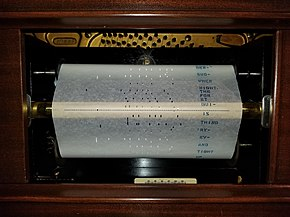
\includegraphics[scale=0.8]{diagrams/PlayerPianoRoll.jpg}
    \caption{A player piano roll, courtesy of Wikimedia Commons.}
    \label{fig:pianoroll} % not attribution, share aliske
\end{figure}

The player piano functions primarily as a traditional piano. There are no alterations made to the timbre or the action of playing the instrument\footnote{The hammers hitting the strings, the triggering of the hammers has indeed be changed in player pianos.} as you would a standard piano. However, additional features have been added to the player piano compared to a completely acoustic one. Player pianos started out being controlled through the use of a large spool of paper, called a roll\cite{plpHist}. Holes punched into this paper would be used to manually trigger levers to actuate the piano's hammer mechanisms and generate sound. Early versions of these instruments were operated with a manual pneumatic pump, operated with the feet\cite{plpHist}. By controlling the tempo and basic parameters of the mechanisms, a "playerist" could perform complex music by operating the foot pedals\cite{plpHist}. Throughout the 20th century, improvements were made to this mechanism including its electrification and eventual digitization\cite{modernPPBasics}. However despite the various technological improvements, a large portion of the market of player pianos is for historic and restored instruments.

The augmentation comes into play when compared to non-player pianos. A completely acoustic piano will not make any sound unless acted upon, and then each individual note must be played in real time to create music. Player pianos are able to perform previously notated music. As the music of Colon Nancarrow (1912-1997) shows, this playback can be significantly more complex than what is possible through human means. Largely known for his work with player pianos, Nancarrow experimented with complex, multi-dimensional canons and tempo relationships between different voices. The end result of which are works for piano that are physically impossible for a traditional performer to reproduce. By utilizing the player piano, Nancarrow was able to embrace this aspect of his music, rather than changing it to match what was traditionally possible.

By being able to play back music, player pianos allowed for a greater spread of music\cite{ppcomod} when audio recording was still in its infancy\footnote{I personally like to view the player piano as analogous to MIDI or similar to MP3 playback of the 1890s}. The instrument's use of permanent, yet technically optional augmentations is similar in nature to that of the electric guitar.

\subsection{ Analog \& Digital Augmentations}
The difference between 20th and 21st century augmented instruments is ambiguous at best. Electrical augmentation is still prevalent in the practice, but as the components become smaller and more affordable, a further increase in the number of instruments can be seen\footnote{Simply scrolling through the archived NIME and ICMC conference proceedings will this growth in the number of papers related to augmented instruments.}. Because digital augmentations are by nature electronic, designating them as analog or digital would prove a better taxonomy than electric vs digital, or 20th century vs 21st. However, determining the most ideal designation of varying augmented instruments is outside the scope of this discussion. As computers increased in power, their usage to both locally and remotely to control augmentation has also increased.

\subsubsection{Electric Guitars Pickups}

The 20th century is when a large number of augmented instruments begin to be developed. This is due in no small part to the development and commercialization of audio amplification and recording during the late 19th and early 20th centuries\cite{recHist}, as well as improvements to those technologies throughout the century. One example of an electronically augmented instrument is the Electric Guitar, which was developed in the 1930's by adding electronic pickups to acoustic guitars\cite{electric_guit_history}. The addition of a pickup is one of the more simple-yet-effective augmentations that can be done to an instrument. The analog signal can be recorded, amplified, or altered with circuitry for a variety of uses both in recording and performing live music. In fact, this is the basic functionality of guitar effect pedals. In practice a pickup is so effective because it is a simple sensor that can be applied to a large variety of processes; a feature shared with the Cyberinet and many other instruments.

\begin{figure}
    \centering
    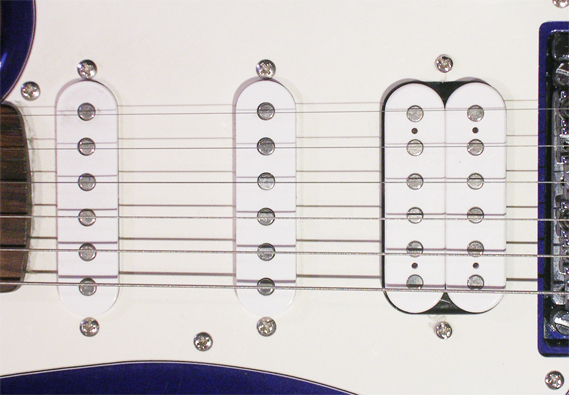
\includegraphics[scale=0.5, angle=180]{diagrams/Pickup-SSH.jpg}
    \caption{Guitar pickups showing magnets underneath each string. Courtesy of Wikimedia Commons.} %public domain image
    \label{fig:pickups}
\end{figure}

Guitar pickups function similarly to dynamic microphones and speaker cones. Each pickup contains a magnet wrapped in a metallic coil placed underneath each string of the guitar. When the metallic strings vibrate, the vibrations cause fluctuations in the magnetic field, resulting in analogous electrical signal to be generated and sent to be altered or amplified\cite{coils09}. Other types of pickups, such as piezoelectric, operate in a slightly different manner, the end end result is the same: an electrical signal is generates and sent somewhere else for manipulation. Electronic pickups are the only analog augmentations to be discussed in this chapter. The remaining instruments are all digitally augmented with various computer processing being integral to the instrument functionality.

\subsubsection{MIGSI}

The Minimally Invasive Gesture Sensing Interface, or MIGSI, Trumpet is an augmented instrument designed to work with the ergonomics and performance practice of the traditional trumpet\cite{reid2016}. Towards this goal, creator Sarah Belle Reid developed a collection of sensors that fit seamlessly into the form factor of B-flat and C trumpets. These sensors work to capture control data including valve placement, hand tension, instrument position. These values are sent wirelessly to a computer to be utilized in digital processing. Infrared sensors are utilized to measure the valve position when fingering various notes, Force-Sensing resistors (FSR's) are used to measure the placement and tension within the hand holding the instrument, and accelerometers measure instrument movement. While the sensors that make up MIGSI are removable, all of the images of the instrument, such as figure \ref{fig:MIGSI}, show that these are held on with bolts, which is not conducive to a quick swap if a performer needed to suddenly remove the augmentation.

MIGSI collects data and transmits to a computer to be utilized in some process. To help with this process, MIGSI is compatible with Max and other programs which can receive serial data\cite{reid2016}. Reid et al. have developed a platform which receives Open Sound Control (OSC) data for a wider range of software compatibility\cite{reid_2019}. In order to demonstrate the effectiveness of the instrument, Reid has written multiple papers on MIGSI, as well as creating several improvisations and compositions utilizing the instrument, such as \textit{Consider} (2017) and \textit{Pocket Fig} (2015).

\begin{figure}
    \centering
    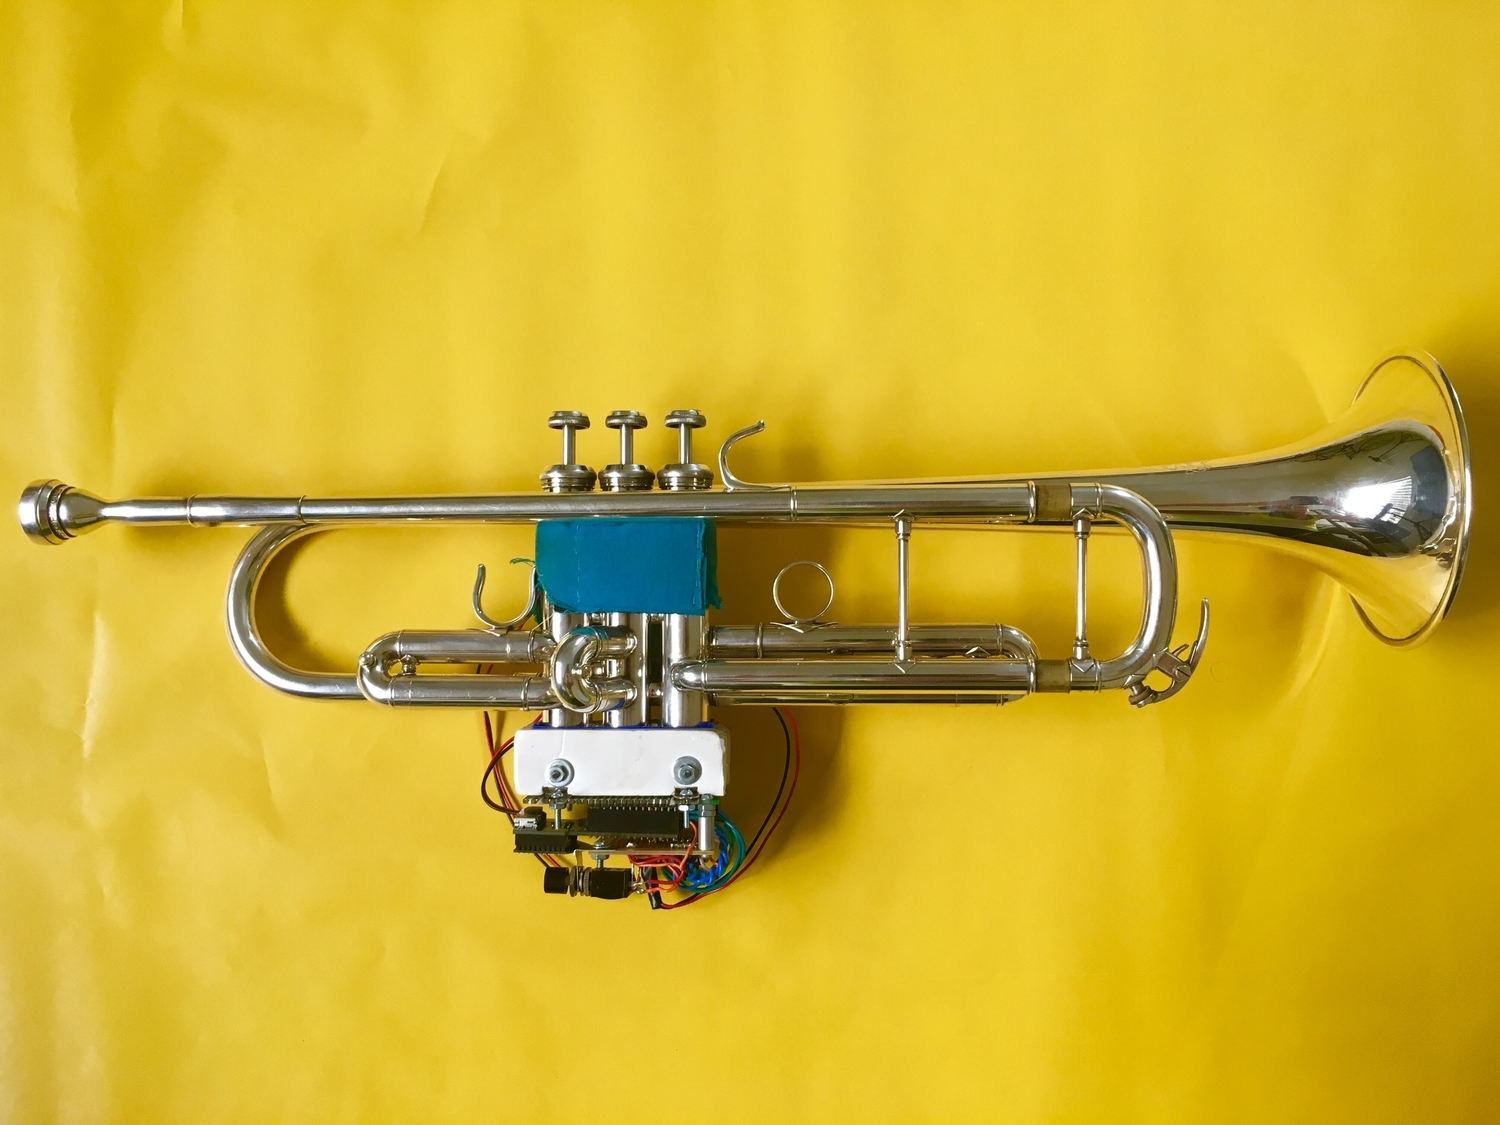
\includegraphics[scale=0.25]{diagrams/MIGSI.jpg}
    \caption{Photo of the MIGSI trumpet, used by permission.}
    \label{fig:MIGSI} % from sarahbellereid.com/migsi
\end{figure}


Here we will discuss \textit{Pocket Fig} for the MIGSI Trumpet, written by Sarah Belle Reid\footnote{A performance video of \textit{Pocket Fig} can be found at \url{https://www.youtube.com/watch?v=5szWkbVjYxg}}. In this semi-improvisatory work, Reid utilizes the FRS's as well as infrared sensors to collect data related to the position and valve displacement on the instrument\cite{reid_2019}. This data is then wirelessly sent to the computer to control a Max patch's granular synthesis processing. The end result is, in Reid's own words from the online performance description: 

\begin{quote}
    "a flurry of classic computer music sounds, stutters, and granular synthesis gestures based on the voice and trumpet sounds of the performer."
\end{quote}

This flurry of effects are heard in performances as soon as the performer releases a trumpet valve\cite{reid_2019}. This gesture triggers a randomized playback of multiple grains taken from the recording of the performance. As the work continues, additional latency between the gesture and effect are intentionally introduced in order to subvert the viewer's expectations and allow for more interplay between the sounds and the performer\cite{reid_2019}.


\subsubsection{SABRe}

The SABRe is another sensor array, but this one is designed to work with the Clarinet, but is also compatible with various other single-reed woodwinds. The unit straps onto the instrument and can be used to collect airflow and position data to be wirelessly sent to a control computer. While effective and easily removable, this particular device offers a relatively limited amount of usable parameters which can be utilized in an augmented instrument. In the majority of cases this is not problematic, as like the MIGSI, the choice in sensors matches with the common performance gestures of the instruments using it, but other devices are needed should a performer have to capture any data that cannot be read by the SABRe. The additional costs of more sensors can potentially be a deterrent to choosing the instrument for use in a composition.

Similar to MIGSI, SABRe is intended to also be minimally invasive to the performer. It is intended for use mainly with Clarinets, being originally prototyped on a Bass Clarinet, but can be easily applied to almost any single-reed instruments\cite{Schiesser2012}. The goal of the SABRe is to provide augmentation features to performers, regardless of their technical abilities\cite{Schiesser2012}. To help with this, SABRe comes with a variety of bands to attach the main unit to different sized instruments. SABRe utilizes four main sensors as well as an additional set of buttons that can wirelessly communicate with the main unit. These include gyroscopic and accelerometer data, airflow sensors, and buttons.\footnote{There are a few more sensors in the SABRe, but the ones mentioned are the main ones advertised.}

\begin{figure}
    \centering
    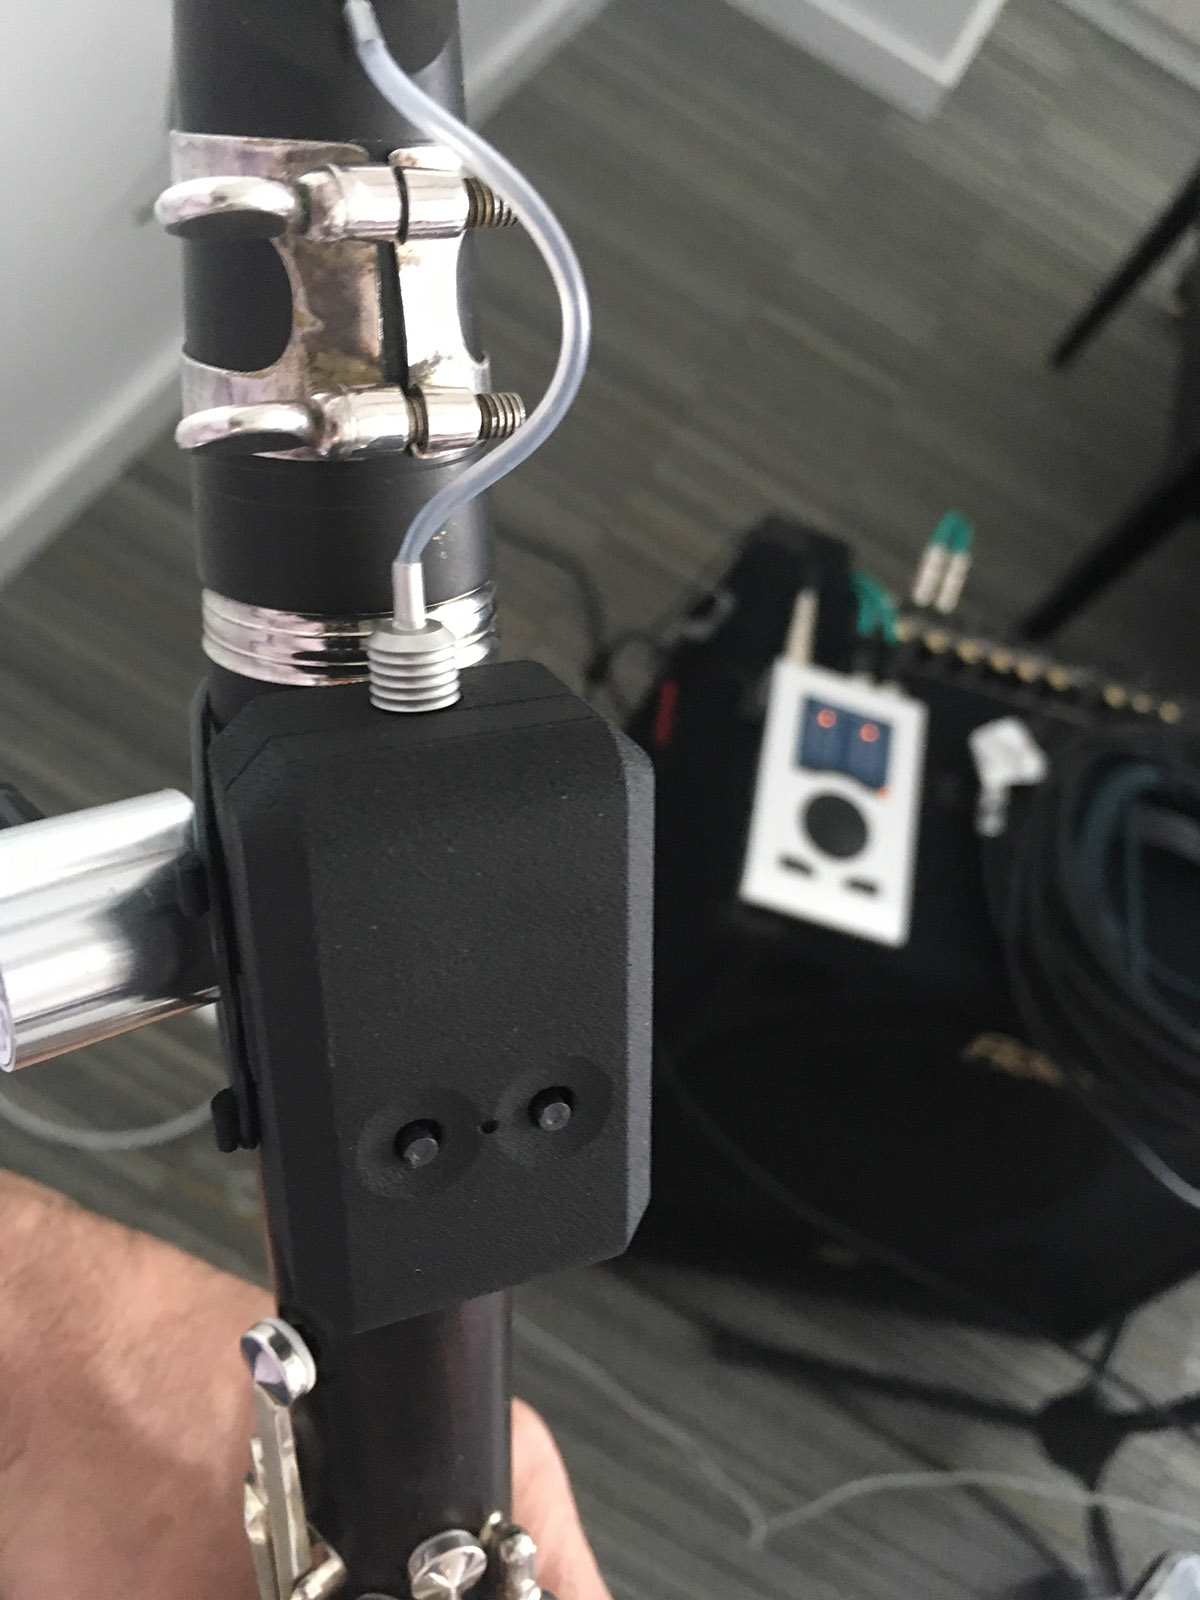
\includegraphics[scale=0.2]{diagrams/sabre-right-hand.jpg}
    \caption{SABRe on a Clarinet, from \url{https://www.jeanfrancoischarles.com/2018/11/first-look-at-sabre-Clarinet-sensor.html}}
    \label{fig:SABRe} % from a blog, no contact information on website.
\end{figure}


SABRe contains a similar base to the Cyberinet in terms of sensors. The main sensors included in the SABRe are a gyroscope and accelerometer which can monitor the performer's movement in real time. There is also an airflow sensor which can detect the air leaving the performer's mouth as it passes the mouthpiece. This is done with a special order mouthpiece pad containing a notch for the sensor tube to rest in. While ingenious in terms of placement, if the pad wears out and the performer is unable to receive a new one from SABRe, then that sensor becomes useless until the pad is replaced since that is all that is holding the airflow tube in position. There are additional sensors as well such as a thermometer, but these are not utilized as much in performance as the aforementioned sensors. Both SABRe and the Cyberinet also have a removable set of buttons that can be triggered as needed by the performer.


Prior to early 2023, SABRe had been on a hiatus in terms of development and is currently in the process of designing a relaunch of the system. It is perhaps for this reason that there is a limited number of works for and writings about the system, but discussing the reasons behind the hiatus is beyond the scope of this paper. Unfortunately however, the majority of resources provided by SABRe online have been taken down and not publicly backed up pending their eventual relaunch of the system. Differences may occur between the original version, discussed here, and the eventual second iteration. The original design utilized a software program developed by SABRe to control the receiving and control of the data for audio processing, as well as being compatible with Max\footnote{This all-in-one software program was built utilizing Max}. 


One piece written for the SABRe is \textit{Sailing}\footnote{The performance of \textit{Sailing} can be found at \url{https://www.youtube.com/watch?v=Eiuacb5nJc8}} by the SABRe's creator: Matthias Mueller. In this work, Mueller takes the gyroscopic information from the SABRe to control audio effects in real time. The first effect heard is reverb and delay. As the performer moves left and right, the amounts of these effects are controlled. This is followed by triggering a tremolo effect that combines with the Clarinet timbre. Due to a lack of a score and other resources due to the aforementioned relaunch of the system, it is my best guess from the video that this effect is being toggled on with the buttons located on the back of the instrument. By combing these effects with micro-tonal notes, Mueller is able to create a unique sound world easily and effectively. Mueller also utilizes a pitch shifting effect, but it is unclear in the video if it is created as a unique harmonizing effect, or is created as a byproduct of adjusting delay times. The final effect is a little distortion present when the performer reaches the extreme ends of the performance area.

In the future, should a performance score or the software patch become publicly available, it would warrant more in depth analysis of the performance practice and specific utilization of the SABRe's sensors. However, there is still much that can be learned with Mueller's performance video. It can be seen that Mueller clearly focusing on only a handful of sensors present within the SABRe: the accelerometer and buttons. By focusing on a smaller subset of the sensors, it allows Mueller to allow the capabilities to the system to stand out. It becomes very clear what the correlation between the Clarinetist's physical position and the timbres being created are.

Mueller's utilization of the button is worth bringing up individually. In \textit{Sailing}, Mueller is most likely using this button to trigger a tremolo-like effect to be applied to the Clarinet's signal. Unfortunately without the software patch or score the fine details of this are left to speculation, but I want to focus on the idea of manually triggering an effect with a button. Unlike a foot pedal, these buttons follow the performer, allowing them to take full advantage of the buttons along with the movement sensors. A performer can access the buttons regardless of their on-stage location. The buttons can also be placed in various locations around the stage if needed, limited only by the length of a cable or the distance of the Bluetooth connection. Having a mixture of continuous and momentary sensors\footnote{The buttons are momentarily on when pressed, while the other sensors are continuously monitoring data values} allows for the performer to create instant (or near instant) changes in the software state like shown with Mueller's triggering of the tremolo effect. Both the Hyper-Flute and the Cyberinet utilize this mixture of momentary buttons with continuous sensors. The continuous sensors can be either digital or analog, that does not effect the relationship between them and the buttons.


\subsubsection{Hyper-Flute}

There are many more augmented instruments that have been developed in the 21st century so far. A full study of them would warrant an entire other dissertation\footnote{A few other examples include the Meta-Sax, Overtone Violin, Haptic Drums, the instruments discussed by Reid et al.\cite{reid2018}, and instruments developed by the Augmented Instruments Laboratory in London.}. Here, we will wrap up our discussion of digitally augmented instruments with the Hyper-Flute.

\begin{figure}
    \centering
    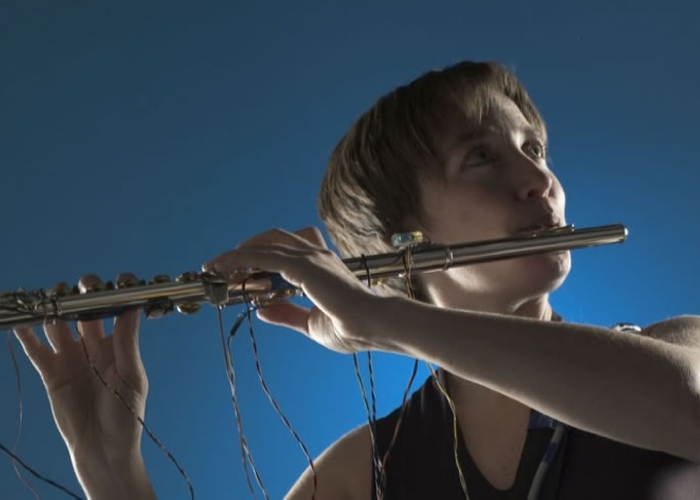
\includegraphics[scale=0.5]{diagrams/palacio_quintin_cleo.jpg}
    \caption{Cléo Palacio-Quintin performing on the Hyper-Flute, used by permission} % https://quasar4.com/en/repertoire/composers/cleo-palacio-quintin
    \label{fig:hyper-flute}
\end{figure}

Developed in 2003 by flutist/improviser/composer Cléo Palacio-Quintin, the Hyper-Flute is a Powell 2100 model flute with a handful of sensors embedded into various locations along the instrument\cite{hyper-flute2003}. Palacio-Quintin's stated goals in developing the instrument are: 

\begin{quote}
    ...[to preserve] the intimate relationship between my body, my instrument and the sound it produces. I wanted to keep intact the acoustic richness of the flute, and my way of playing it. The computer had to become a virtual extension of the acoustic instrument \cite{hyper-flute2003}.
\end{quote}

Towards this goal, Palacio-Quintin ultimately decided on six unique sensors that can control the computer processing of the flute. While there are some overlaps between the Hyper-Flute and the other instruments discussed in this chapter, the design implements a variety of unique ideas not present in the other wind instrument augmentations discussed. Firstly is that the Hyper-Flute is not a removable augmentation like the Cyberinet, SABRe, or MIGSI. These sensors, listed in figure \ref{fig:hyper-flute-sensors}, are permanently installed onto the flute. 

During a performance, voltages from each of these analog sensors are analyzed and converted to a MIDI value which can be sent to a computer or any MIDI compliant instrument. All of the data is sent as control MIDI messages. A feature that is particularly interesting about the Hyper-Flute is that while Palacio-Quintin has developed various software patches using Max, similarly to the other digitally augmented instruments discussed in this chapter, the instrument does not rely on the software. Because the data being generated is MIDI compliant, the Hyper-Flute can easily interface with a large variety of instruments via the MIDI port, which can open an entirely different world of performance practice and possibilities when compared to other instruments\cite{hyper-flute2003}. Unique to the other instruments discussed throughout this chapter, the Hyper-Flute requires a separate interface in order to convert the voltages into MIDI data. Palacio-Quintin utilizes a Microlab interface for this purpose. This is a custom device created by A.J.van den Broek\cite{hyper-flute2003}. 

\begin{figure}
    \centering
    \begin{enumerate}
        \item Magnetic field sensors to detect pinkie-key movement.
        \item Ultrasonic distance sensor to detect distance from the computer.
        \item Tilt switches to detect movement and rotation of the instrument.
        \item Pressure sensors located where the performer holds the instrument.
        \item Light sensor to detect ambient lighting changes.
        \item Button switches which can be activated by the thumbs while performing.
    \end{enumerate}
    \caption{Sensors present in the Hyper-Flute.}
    \label{fig:hyper-flute-sensors}
\end{figure}

In musical performance, the use of sensors can be seen in \textit{Souffles Électriques}, a small collection of various works for the Hyper-Flute.\footnote{\textit{Souffles Électriques} can be found online at\url{https://vimeo.com/155153474}.} While not discussed in the original 2003 paper, Palacio-Quintin has since expanded the range of instruments to include at least the Bass Flute as well as the original Concert Flute, as shown in the performance video. The performer is able to intuitively control the sounds from the various sensors. Effects such as adjusting audio processing and the playback of samples by pivoting the flute angles and position in three dimensions are seen in the performance, as well as the use of the magnetic field sensors in the pinkie keys.

\newpage

\section{Cybernetics \& Music}
While not a design feature of every augmented instrument, many of ones discussed, especially those of a digital nature, allow for a level of Cybernetic interaction between the performer and the music. Much like electronically augmented instruments, Cybernetics is a relatively modern science with roots going back centuries. The core principals of which have brought about advancements in various fields such as mechanics, philosophy, health management, music, and more. 

\subsection{General Cybernetic Concepts} %% This needs a graphic of something in this subsection partway through.

The concept of modern cybernetics was defined by Norbert Wiener in his 1948 book \textit{Cybernetics: Or Control and Communication in the Animal and the Machine}, which has had its second edition republished in 2019\cite{WeinerCybernetics2019}. The republished versions contain additional supplementary chapters not included in the original 1948 publication. In its original context, Cybernetics is defined by Wiener as: 

\begin{quote}
    "The science of communications and automatic control systems in both machines and living things."
\end{quote} 

While the concepts of Cybernetics were present before Wiener, it was in his writings that the term "Cybernetic" was formally created. The term is derived from the Greek kubernetes, which approximately translates to "the captain of a ship"\cite{WeinerCybernetics2019}. Wiener credits J.C. Maxwell in his 1868 paper as one of the first formal studies into what would ultimately evolve into Cybernetics. In that paper, Maxwell discusses the concept of a Governor and Moderator within a variety of mechanical systems\cite{maxwellOnGoverners}. Wiener posits that perhaps one of the earliest examples of the work as described by Maxwell is that of the steering mechanism of a boat\cite{WeinerCybernetics2019}. Heavily summarized, this is the idea that a sailor on a boat can see and respond to the conditions they are sailing in by turning the wheel, which, through mechanical means described by Maxwell\footnote{Maxwell's original article is largely composed of complex mathematical operations based on hypothetical systems, the specifics of which is beyond the scope of this document.}, causes the boat to turn, thus altering its condition and allowing the sailor to be able to respond to the new condition.

As time progressed, the definition of Cybernetics has evolved. Scientifically, the definition is relatively unchanged, still focusing on feedback systems and automated responses, but now is utilized in the development of artificial neural networks and machine learning\cite{Cariani2010}. In popular culture, Cybernetics often invoke ideas of half-organic/half-machine creatures. This connection is partly due to these creatures' name: "Cyborg". This word is a portmanteau of cybernetic and organism. The mechanical components present in these beings are able to react to the state of the organic components and either enforce or act against what is happening in the body. A few examples of cyborgs in popular media are the Cybermen from \textit{Doctor Who}, the Borg from \textit{Star Trek}, RoboCop, Motoko Kusanagi from \textit{Ghost in the Shell}, Darth Vader from \emph{Star Wars}, and Numbers 17 and 18 from \textit{Dragon Ball Z}. All of these examples have utilized automated, mechanical components to augment some part of their body, although the level of these augmentations largely is still only possible in the realm of science fiction.

A real-world version of this is present in modern diabetes management systems such as the Omnipod 5 or Medtronic MiniMed. Looking specifically at the Omnipod\footnote{I actually have personal experience utilizing the Omnipod 5 in order to accurately manage my Type One Diabetes. This was in no small part an inspiration for the ultimate direction of the Cyberinet.}, this insulin delivery device has the capability to be paired with a constant glucose monitor (CGM) embedded within the user's abdomen. CGM will read the glucose levels of the user and automatically adjust the Omnipod 5's insulin delivery rate to compensate for any changes to the blood glucose levels, and adapts its changes based on daily insulin dosages. This system is cybernetic in every sense of the word. It combines organic and inorganic components like in popular culture, as well as the internal feedback loops to control the blood glucose level of a diabetic as in the scientific definition, in a manner similar to a person without diabetes.

\begin{figure} % Need a graphic for this, but may have to make one since this is a major company
    \centering
    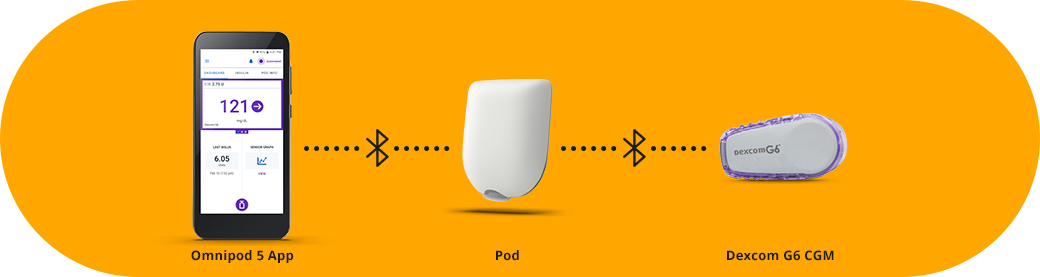
\includegraphics[scale=0.4]{diagrams/Omnipod-5_CGM_Pod_BT_1040x277.jpg}
    \caption{Diagram made by Omnipod showing the communication of the Omnipod 5.} %what can I do as another option?  I have the hardware
    \label{fig:omnipod}
\end{figure}

Cybernetic concepts such as feedback loops and automatic responses are heavily utilized in Cybernetic music. The idea of the music becoming a sort of living thing that is able to grow and change on its own, or develop a unique, self-aware character is appealing to many composers of the 20th and 21st century. Many other composers would also direct this evolving music in order to create more desirable creative results. In addition to being an augmented instrument, the Cyberinet utilizes Cybernetic principles in its design and intended uses. 

Another Cybernetic concept which is present in music composition of the 20th century is that of second-order cybernetics. The core differences between first and second order cybernetics is the inclusion of the observer within the cybernetic system. Rather than a completely isolated system, a person in a second-order cybernetic system is able to observe and react, altering the system and controlling the output to various degrees. In terms of musical composition, this allows for a composer to both allow for the unique characteristics of cybernetic systems, but still control the output enough to give the final result their own unique flair. One of example of this is Terry Riley's \textit{In C} or Fredrick Rzewski's \textit{Les Moutons de Panurge}. Both of these acoustic 20th century work have performers playing musical snippets, but are independent of each other. As the performers become less in-sync, they are able to make more choices that affect their performance, and how they are interacting with the group as a whole.


\subsection{Cybernetic Music Practices}
As previously mentioned, cybernetic principals have also been utilized in music composition. Various composers have utilized Cybernetic ideas to create music that can evolve over time. These effects can give the music a unique character and identity. Implementing cybernetic music can happen through both entirely acoustic means, as well as through computer controlled algorithms. This subsection will discuss three composers who utilized Cybernetic in various ways, as well as how those concepts were utilized within a specific composition.


\subsubsection{Herbert Brün}

Born in 1918, Brün was both a composer and computer scientist who focused on Cybernetic concepts in his various works. Many of these works were programmed in early coding languages such as FORTRAN which allowed Brün to incorporate both randomness and Cybernetic feedback into the music generation process. In a handful of works, such as \textit{mutatis mutandis} from 1968, would utilize random number seeds in order to create visuals which were then interpreted by musicians.

In relation to Cybernetics, Brün was influential in the development of Second-Order Cybernetics along with other scientists such as Heinz Von Forester and Margaret Mead. Second-Order Cybernetics ultimately developed into a process which is heavily utilized in Cybernetic music moving forward. In short, the main feature of Second-Order Cybernetics is the inclusion of the observer in the Cybernetic system, as opposed to them existing outside of it\cite{Scott_2nd_order_Cyber}. In relation to the creation of music, this meant that a composer utilizing this concept would be able to create a cybernetic system, and then directly influence it in order to affect the outcome.

During his tenure at the University of Illinois, Brün taught a mixture of music and computer science courses. His work with the Electronic Music Studio, helped to expand a variety of computer music concepts. One of these is the creation and continued development of gesture-based computer synthesis. 
SAWDUST, MORE INFO AND MUSIC. BASICALLY MADE COMPUTER MUSIC OUT OF ELECTRONIC MUSIC. TYPES OF SYNTHESIS.

\subsubsection{Roland Kayn} % more biography. try and find more detailed information on composition. headshot

A German born composer, born in 1933, who was heavily inspired by information sciences when creating his unique style of mainly electronic and electroacoustic music\cite{rolandKaynBio}. His earliest works to utilize the cybernetic concepts was \textit{Galaxis} (1962) for a variable acoustic instrumental ensemble and \textit{Cybernetic} (1969) for electronics. Kayn would write several more over the following years. These works incorporated cybernetic principals in what Kayn referred to as being "self-governing"\cite{rolandKaynBio} and "able to think for itself\cite{Kayn_Elektroakustische_Projekte}. In the context of Kayn's electronic music, this was present in algorithmic processes which incorporated semi-random calculations. These unpredictable results were then fed back into the system which resulted in unpredictable, autonomous results\cite{rolandKaynBio}.

\begin{figure}
    \centering % get permission for score page
    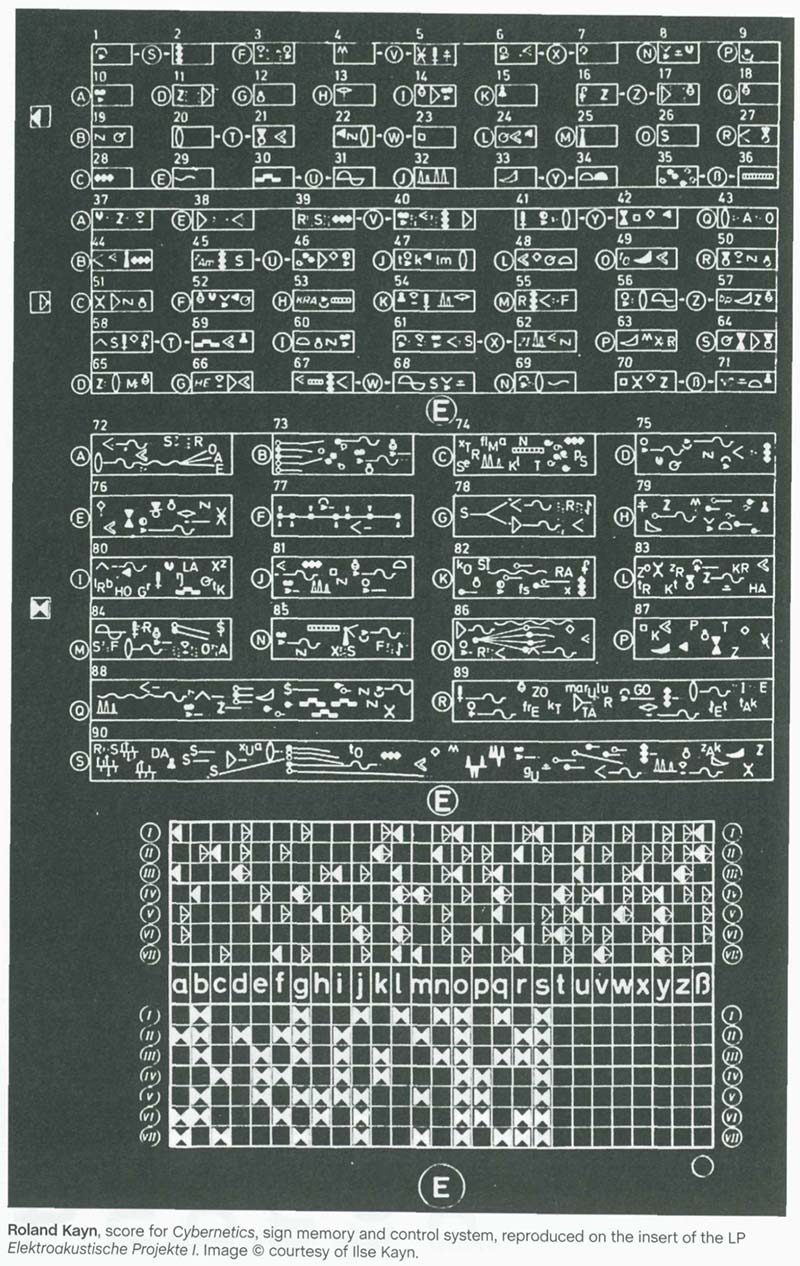
\includegraphics[scale=0.45]{diagrams/kayn_cybernetics.jpeg}
    \caption{\textit{Cybernetics I} (1969) score, Courtesy of Ilse Kayn, used by permission}
    \label{cyberneticsScore}
\end{figure}


Figure \ref{cyberneticsScore} shows one of Kayn's works, \textit{Cybernetics I} from 1969, and shows the various electronic components used to generate the sound in the top portion, and how those components interact in the bottom portion, similar to the matrices used in synthesizers of the era. Looking at the score, we can see how the output of certain processes are fed back into the system, causing the feedback loops common to Cybernetic music.


\subsubsection{Pauline Oliveros} % show page of sonic meditations
An American composer, performer, and educator, Oliveros was a founder of the San Francisco Tape Music Center and pioneer of\textit{ Deep Listening}\cite{HolmesElectronicMusic2020}. \textit{Deep Listening} is a school of thought at method of listening described by Oliveros as:

\begin{quote}
    ... For me [Oliveros], Deep Listening is a lifelong practice. The more I listen the more I learn to listen. Deep Listening involves going below the surface of what is heard, expanding the whole field of sound while finding focus. This is the way to Connect with the acoustic environment, all that inhabits it , and all there it.

    For others, Deep Listening is a practice consisting of listening and sounding exercises and pieces I and others have composed since 1970. The results are proceeded by a group of discussions in workshops and retreats. 

    Deep Listening is for musicians as well as participants from other disciplines and interests. Previous musical training is not required\cite{cultureandHumanity2002}.
\end{quote}

At its core, the idea of \textit{Deep Listening} itself is a cybernetic practice\cite{gordosOliverosCybernetics}. This is because of \textit{Deep Listening}'s core principle of listening to how you listen. The act of a system responding to itself in a feedback loop is a core concept in cybernetics. In relation to Olivero's music, the concepts of deep listening and cybernetics can be clearly seen in her tape improvisations of the 1950's and 60's. In these works Oliveros along with a variety of collaborators would record themselves improvising, then listen to the recording and discuss what they heard. Following this the group would repeat the process until they were pleased with the results\cite{gordosOliverosCybernetics}. 

% \begin{figure}
%     \centering % get permission: Pauline Oliveros. Credits: Bert Johnson. But who do I email? there are many Bert JOhnsons https://eastbayexpress.com/avant-garde-luminary-pauline-oliveros-listens-deeply-to-the-berkeley-art-museum-1/
%     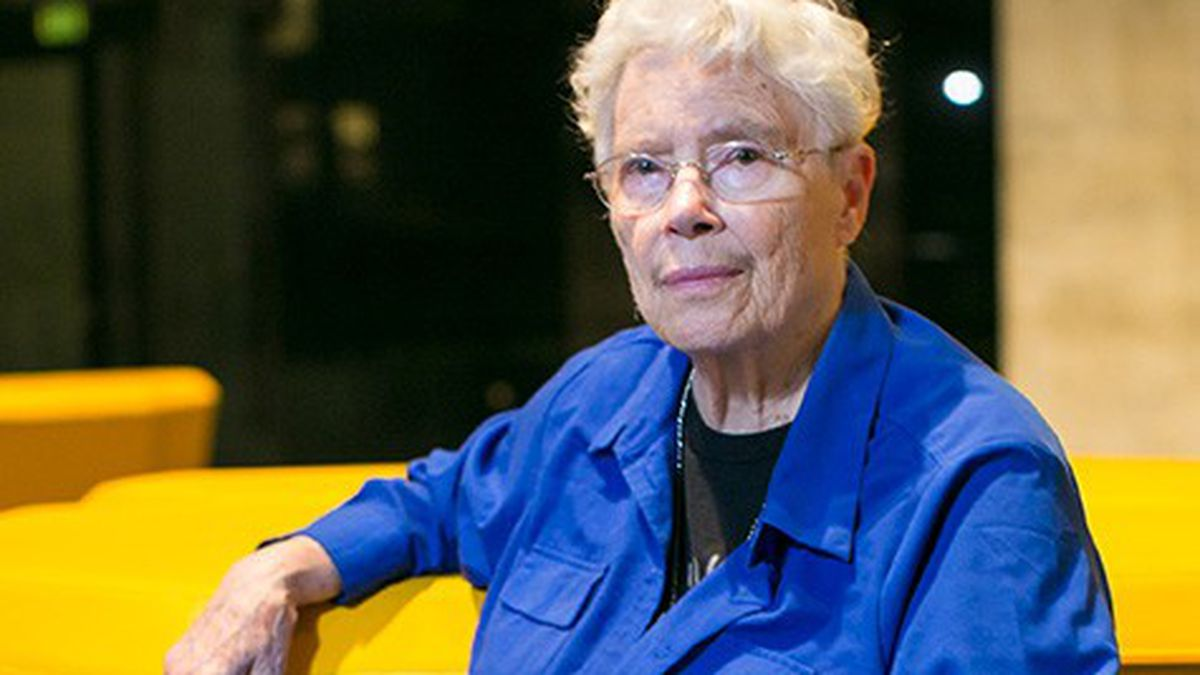
\includegraphics[scale=0.25]{diagrams/oliveros.jpg}
%     \caption{Pauline Oliveros}
%     \label{fig:oliverosHS}
% \end{figure}

Another series of works with cybernetic principles is Olivero's \textit{Sonic Meditations} (1974). \textit{Sonic Meditations} is a collection of 25 different actions intended to cause the performer to intensely focus on their action, the sounds around them, and the sounds of their actions\cite{OliverosMeditations}. The instructions are all given as text have been performed in a traditional setting or individually, but in the score Oliveros intends to remove nay connotation of traditional performance and focus on the sound through \textit{Deep Listening.} 

These prompts range in complexity and specificity ranging from talking a walk with as quiet of steps as possible to singing pitches in groups until a single pitch is established. There are also more complex activities focused on breathing and the acts of making, listening to, imagining, and remembering sounds\cite{OliverosMeditations}. By actively guiding the performer through the \textit{Deep Listening} activities, all of the cybernetic principles of \textit{Deep Listening} become present in the music performance as well. All 25 pieces have in some way the performer listening to a sound occurrence and responding by altering their actions to change the sound environment.

\subsubsection{Onyx Ashanti} 
Onyx Ashanti is a modern composer, performer, and inventor largely known for developing "beatjazz", an electronic gesture controller used to utilize a mixture of improvisation, looping, and gestural control. These gestures are incorporated through his instruments, which directly attach to the human body. A few sensors are even located within the performer's mouth. These particular arrangements of data work to remove some of the traditional aspects of music creation and performance and allow for the creation and control of audio to happen solely through the direct measurement of the performer.

The Beatjazz controllers are held in the performer's hands and utilize accelerometers in order to track the positional data of each hand, FSRs to monitor finger pressure both as buttons and continually, and a wind sensor placed in the performer's mouth\footnote{Stock non-withstanding, all of the parts for the original Beatjazz controller can be ordered as a set directly from.}. The system is controlled through a computer running the various software patches for each performance. In terms of feedback, Beatjazz utilized a paired smartphone in order to act as a GUI for the performerer. LED's on each sensor allow for the user to easily see which parameter they are controlling using the following setup:

\begin{table}[]
    \centering
    \begin{tabular}{|c||c|}
    \hline
      red   & drums \\
      \hline
      blue   &  bass\\
      \hline
      green & chords \\
      \hline
      orange & leads\\
      \hline
      purple & pads\\
      \hline
    \end{tabular}
    \caption{LED color feedback in BeatJazz}
    \label{tab:bjLEDs}
\end{table}


The most interesting aspect of Beatjazz is that it removes the need for a traditional instrument or control interface in order to create music in real time. By ergonomically fitting onto the performer, their physical actions are directly used in order to alter the musical environment. By altering how they are moving, the performer can directly change what samples are being used and how they are being digitally processed. This allows for Beatjazz to function cybernetically both in the popular culture and scientific uses of the word. However, because of how it is utilized on the body, it is less of an augmented instrument than something completely new, which has many common similarities with digital augmented instruments.

\section{The Cyberinet}
Taking everything up to this point into consideration, and the main definitions and goals of the Cyberinet can be clearly broken down. When comparing it to the digitally augmented instruments, there are several features that the Cyberinet iterates on, and several that it intentionally does not embody.

In relation to MIGSI, the Cyberinet is also designed to be minimally invasive. While a performer can interact with the instruments in novel ways to create interesting effects through the various sensor data, utilizing MIGSI and the Cyberinet by itself does not impede the traditional performance practice of the performer. Other than instrument compatibility, the main way that the Cyberinet differs from MIGSI is that the Cyberinet is designed to be easily installed and removed, allowing the performer to choose whether their instrument is completely acoustic or augmented. While a performer can choose not to connect MIGSI to the computer, making it acoustic, the MIGSI sensors are not easily removable. Looking at figure \ref{fig:MIGSI}, the sensors are bolted or otherwise securely attached to the base trumpet. When defining the Cyberinet, it was a goal to create a device that would not require a permanent alteration to the instrument, and was in fact able to be quickly implemented in a performance setting like a brass mute. Permanent alterations could be potentially off-putting to musicians. who may be unable to afford a second instrument to augment, or are otherwise unwilling to permanently alter their horn.

The Hyper-Flute is able to interact with a variety of devices or the computer through its Metalab interface and a MIDI port\footnote{This is my favorite feature of the Hyper-Flute, even if the interface results in an additional hardware purchase needed in order to perform with the instrument on top of already having to permanently add the sensors to your flute or buying a separate one to augment.}. While not identical, the Cyberinet software is intended to be able to interact with a variety of hardware and software using Max as the main platform. However, the large number of wires hanging from the Hyper-Flute are both distracting in a performance setting, and can potentially obstruct the performer's movement\footnote{A portion of this drawback is due to the development of more powerful and smaller digital sensors in the 20 years between the development of the Hyper-Flute and the Cyberinet}. The Cyberinet wirelessly communicates with the computer with only external wires needed to connect to optional expansion sensors or to charge the Cyberinet.


Of the discussed instruments, the SABRe is the device most closely related to the Cyberinet. This is in no small part due to the fact that they are designed to augment the same instrument. This also lead to common types of sensors between the two as the sensors are monitoring the same actions. These similarities require a more in-depth breakdown in order to properly differentiate the two devices. Despite being designed for the same instrument, each device has its own unique positive and negative aspects.


\begin{table}[]
    \centering
    \begin{tabular}{|c||c|}
    \hline
     SABRe & \textbf{Pros}: small, completely wireless, easily removable. \\
         & \textbf{Cons}: no modularity, cost, \\
         & buttons difficult to use without the thumb expansion.\\
         \hline
    Cyberinet & \textbf{Pros}: integrated within the instrument,\\
    & expandable with add-ons,\\ 
    & relatively inexpensive to produce, open source-components.\\
    & \textbf{Cons}: less easily removable, \\
    & some wires involved, annoyingly complex to install.\\
    \hline
    \end{tabular}
    \caption{Pros and Cons of the SABRe and Cyberinet}
    \label{tab:sabreCyberinetProCons}
\end{table}



in regards to the SABRe, while extremely simple to set up and utilize, the lack of additional sensors could hamper potential uses. The chosen sensors are all useful in collecting Clarinet performance data, but it cannot be customized outside of adding two buttons to the version one system. To help avoid this potential limitation in the Cyberinet, the Cyberinet is designed to be able to attach an expansion unit with an additional sensor\footnote{This was also done in order to help differentiate the Cyberinet from the SABRe in terms of design and functionality.}. These sensors are all compatible with OEM components and utilize the same voltage ranges. This allows them to be easily swappable in a performance setting.

The final aspect of the SABRe that the Cyberinet intentionally differs from, other than physical design, is the cost. The initial version of the Cyberinet is designed to be completely open-source, utilizing OEM components. While this does increase the overall size of the Cyberinet, it results in a final unit that is significantly cheaper to manufacture than the SABRe. The initial version of the SABRe retailed for approximately €500. All of the components for the Cyberinet: sensors, PCBs, connectors, and 3D printer filament cost approximately \$120. A retail price would be higher, but still significantly lower than that of the SABRe. Even with a 100\% markup, the final cost of the Cyberinet, is less than half that of the SABRe. By having a cheaper development cost, the Cyberinet has a lower cost-of-entry wall, making the unit significantly more accessible than the SABRe. In fact, is a person already has a 3D printer, then they can completely create and program a Cyberinet from scratch for only the cost of the materials.

%%%%%%%%%%%%%%%%%%% define the categorizations?
In the article \textit{Mapping, in digital instruments}\cite{vanNortMapping2007}, Van Nort describes Digital Musical Instruments as being either implicit or explicit in regards to their use of the control data. Where explicit designs are analytically described and implicit interactions are applied through some sort of training\cite{vanNortMapping2007}. In his paper, Van Nort goes on to describe a handful of other interactions between the data being collected and the sound being produced. Using the terms defined there, the Cyberinet can be described as using an implicit, dynamic, and continuous use of the performance gestures for its computer augmentation. Controls are based on Clarinet performance practice and not a new set of skills, the sensor types can change through its designed modularity, and the sensor data is continuously being collected while in use. There is also a multiple layers of mapping between the raw data and what is utilized to produce sound. This is to help further draw correlations for gesture recognition as well as ease of use when programming.

Looking back at the instruments discussed previously in this chapter, we can see many of the instruments share similarities with the Cyberinet in this design choice. While none of the aforementioned instruments would be considered dynamic for exactly the same reason as the Cyberinet, they all collect continuous data using implicit means. The Hyper-Flute specifically has the ability to the data to MIDI for use in other devices,but all four instruments can have the data further mapped within the Max software. Due to the ability for the mapping to change within the software environment for all four of these instruments, each one is capable of adapting and changing the mappings in real time, an act which Van Nort describes as the mapping becoming playable itself\cite{vanNortMapping2007} in a fashion similar to the idea of Second-Order cybernetics.

As stated, the Cyberinet can be defined as a new augmented instrument which can be implemented with a standard B-flat Clarinet. This augmented instrument collects data from various embedded sensors and transmits the data to a nearby computer while the performer plays the instrument traditionally\footnote{Or not. The gestures being captured can be experimented with in order to develop unique sound possibilities.}. The sensors can be adjusted in a semi-modular fashion; by adding or removing expansions to the two main ports on the main unit. The Cyberinet is intended to be affordable to produce, using OEM components with open-source resources. This is to allow for more accessibility to a wider range of performers and composers wishing to work in electroacoustic music. Lastly, because of the Cyberinet being able to control audio processing through the act of performing on the Clarinet, it brings a level of Cybernetic awareness to the performer as well. A performer will be able to play and hear how their actions are influencing the music and either positively or negatively reinforce that control by adjusting their playing in real time. 

But how exactly will the performer be able to influence their playing? A performer composer or performer could create specific movements at specific times to trigger an effect, this could be pre-planned or improvised. A student could monitor the data while learning the instrument to check their positions and breath control. The potential for sound and control options are astronomically high, but there are a handful of useful methods and interactions envisioned by the author, which can help guide newcomers to the Cyberinet. Before we dive into exactly how it is used, Let us first discuss how the Cyberinet was designed, assembled, and programmed.


\chapter{Building the Cyberinet}
When developing the functionality of the Cyberinet, the steps defined by Miranda and Wanderley in their book\cite{miranda_Wanderley_instrumentControl_2006} helped to organize and streamline to process. Paraphrased, that process is shown in table \ref{fig:DMIProcess}. This chapter will utilize the process given here by Miranda and Wanderley as a road map to breakdown exactly how the Cyberinet was designed and created. The core concepts utilized when designing the instrument is to automatically collect and wirelessly transfer data, to be easily implementable without permanent alterations to the Clarinet base, and to be affordably produced.

These self-imposed requirements were largely brought about through the selection of various OEM components that can easily interface with a micro-controller. These components are soldered into a custom-designed printed circuit board (PCB), and housed within a 3D printed replacement for the Clarinet barrel. The entire Cyberinet unit is battery-powered, allowing for its use to be completely wireless, unless expansion units are required. By utilizing these expansion units, the performer can modularly adjust the sensor capabilities to fit their needs.

\begin{table}[]
    \centering
    \begin{tabular}{|c||c|}
    \hline
     Step 1    & Determine gestures that will control the instrument. \\
     \hline
     Step 2    & Determine how to capture the gestures for use within the system. \\
     \hline
     Step 3    & Define the sound creation processes used. \\\hline
     Step 4    &  Map the gesture control data to the desired sound-creation parameters.  \\
     \hline
     Step 5    &  Decide on the feedback mechanisms for the performer.\\
     \hline
    \end{tabular}
    \caption{DMI design steps as defined by Miranda \& Wanderley\cite{miranda_Wanderley_instrumentControl_2006}.}
    \label{fig:DMIProcess}
\end{table}

\newpage

\section{Control Gestures \& Gesture Sensing}
The main control parameters for the Cyberinet are those already present traditional Clarinet performance. While conceptualized as something new, the Cyberinet, as an augmented instrument must still retain its identity as the original instrument\cite{miranda_Wanderley_instrumentControl_2006}. Towards this goal, a breakdown of a Clarinet performance is needed in order to see which gestures are naturally occurring so that they can serve as a starting point for developing more experimental, intentional gestures that to be utilized in composing new works.

In a Clarinet performance, there are a handful of easily measurable actions that occur. The main ones chosen for the Cyberinet are performer movement, which can often be tied to expressiveness\cite{wanderleyClarinetGesture2005}, and performer dynamics, which can be tied to the volume of air flowing through the instrument. Other parameters exist as well such as determining which keys are being pressed, how hard the keys are being pressed, and which pitch is being produced by the Clarinet. While interesting, measuring these data points in real time becomes more problematic due to the necessary placement of sensors and microphones which would impede the performance or alter the instrument into something similar, but distinct from the original Clarinet. Because of these reasons, the movement gestures are the primary focus of the Cyberinet's main unit, followed closely by measuring the air flowing through the horn.

When performing on the Clarinet, the performer generally will pivot or sway horizontally (left-to-right) as they are performing. These motions are the primary focus of the gyroscopic and position sensors as they are both common to see, and natural to produce\cite{wanderleyClarinetGesture2005}. Performers can also lean forward or back while performing, necessitating a need for a second degree of motion when choosing the sensor. It is relatively unlikely that a performer will have significant alterations to the vertical height of the instrument while performing traditionally, however conceptualizing the Cyberinet as a unique instrument separate from the Clarinet opens up the possibility of performance control to traditionally unused actions. Because of this, the Z-axis is also monitored by the chosen gyroscope and accelerometer. 

The second sensor embedded within the Cyberinet's main unit is a differential airflow pressure sensor. This sensor was chosen as a way to directly measure the airflow within the instrument. As a performer creates notes at different dynamics, the volume of air flowing through the instrument will change. By comparing the pressure within the horn with the air pressure outside of the instrument, these values can be easily calculated as a number to utilize in the code. 

With the general gestures of movement aid airflow, and the requirements for sensors determined, the next step is to work out a more specific list of gestures to begin testing. In 2005 Wanderley et al. conducted a study in order to determine both what expressive gestures were present in Clarinet performance, as well as how these gestures can affect music performance and perception\cite{wanderleyClarinetGesture2005}. The gestures identified in this study serve as a wonderful baseline for identifying specific movement possibilities. Summarized, these natural expressive performance are listed in table \ref{tab:generalGestures}.

\begin{table}[]
    \centering
    \begin{tabular}{|c||c|}
    \hline
       Instrument Movements  & Bell, vertical and circular \\
       \hline
        Upper Body Movements & Head, vertical \\
        & Shoulders, vertical \\
        & Back, curl inwards \\
        & Arms, raising elbows \\
        \hline
        Lower Body Movements & Waist, bending \\
        & Knees, bending \\
        & Feet, walking \\
        & Weight shifting, left and right\\
        \hline
    \end{tabular}
    \caption{Identified Gestures by Wanderley et al.\cite{wanderleyClarinetGesture2005}, divided by body area.}
    \label{tab:generalGestures}
\end{table}

These natural gestures are all able to be measured with the Cyberinet. Rotations are easily picked up by the gyroscope, movements by the accelerometer, and breath by the airflow sensor. While Wanderley et al. did not measure the airflow in their study, it is still an important sound-producing gesture\cite{miranda_Wanderley_instrumentControl_2006}. Each of the gestures listed above as well as a handful of airflow gestures were tested with the Cyberinet in order to calculate the various sensor responses to various scenarios. This data was then used to create Max objects that can utilize both slower, gradual movements, as well as faster ones that can be be interpreted as a single action.

%should I move the breakdown of geasutes adn thier data visualizations to here?

\subsection{Gesture Mapping}

Because of the modularity of the programming environment, a single gesture sensed by the Cyberinet can be mapped to anything within Max. This leads to a few unique concerns; mainly the idea of determining the most effective parameters to map to an effect. This design feature is intended to create a wide variety in potential outcomes without the need for the performer to learn an equally large number of control actions. This potentially overwhelming amount of options is made more manageable with the use of a normalized value range for the sensors and a collection of Max objects that either process sound or help prepare the use of the data for use in other ways. 

When deciding which gesture is effective for an effect depends on a few parameters. The first one is purely mathematical: if a parameter utilized large changes in values, then a similar data profile will prove more effective than others. An example of this would be calculating exponential growth for applying data to a range of frequencies on a filter or equalizer. A quick gesture will prove best for a quick change or process within Max, whereas slower changes in data values are better applied to continuous audio processed, Such as activating a gate with a short gesture versus controlling the pitch of a synthesizer with a longer movement gesture. 

The second parameter depends on the performer. People will naturally perform differing natural movement when performing\cite{wanderleyClarinetGesture2005}, which could result in varying sensor responses between users. Because of this an object in Mac, called CNET.rangeSet, was created in order to adjust the scaling of values as needed for each performer. This way, with minimal setup, the sensitivity of each continuous sensor in the Cyberinet can be scaled to match the movements of varying performers in order to achieve a consistent performance effect.

\subsubsection{Visualizing Gestures within Max}

The idea of mapping physical gestures to the sound production/processing created by an augmented has already come up a few times. While indeed this can be done haphazardly or randomly, in order to properly utilize the cybernetic capabilities of the Cyberinet (or any other digital musical instrument), the performer must be able to respond to the current state they are in and create either a positive or negative feedback loop to maintain, grow, or diminish the current state. In order to do this, it is important to identify gestures being used and how they are mapped. Generally speaking, a gesture can be traditional or experimental in nature. Each of the gestures in table \ref{tab:generalGestures} have been analyzed and visualized for easier application to sensors.

To create this data, the CNET.gestureVisualizer object was used to record the sensors values while the movements were performed. The data was then represented with the multislider object in Max. The categorization of the gestures was based on this visual representation. When looking at all of the data points, the oldest points are presented on the right of each graph, and the newest points are on the left. Because of the manual trigger to start and stop recording, extra noise is present on the right-most 10\% of each graph, and should be ignored. 

Throughout all of the data graphs, the Gyroscopic Z-axis values appear more sensitive than the majority of the others. This is due to the positioning of the sensor on the instrument. Longitudinally, all of the motion sensors of the Cyberinet are close to the center of motion in the Cyberinet. However, transversely the sensor is located approximately 9 inches away from the center of motion\footnote{The center of motion is considered to be the thumb-rest/neck-strap attachment point in the center of the instrument.}. Because of this larger distance, the sensors which respond to that axis will register a larger change in position. This can be adjusted slightly by rotating the Cyberinet main unit on the horn, but utilizing CNET.rangeSet will better scale the values as desired. All of the graphs shown here are utilizing unaltered data from CNET.receive.

\begin{figure}
    \centering
    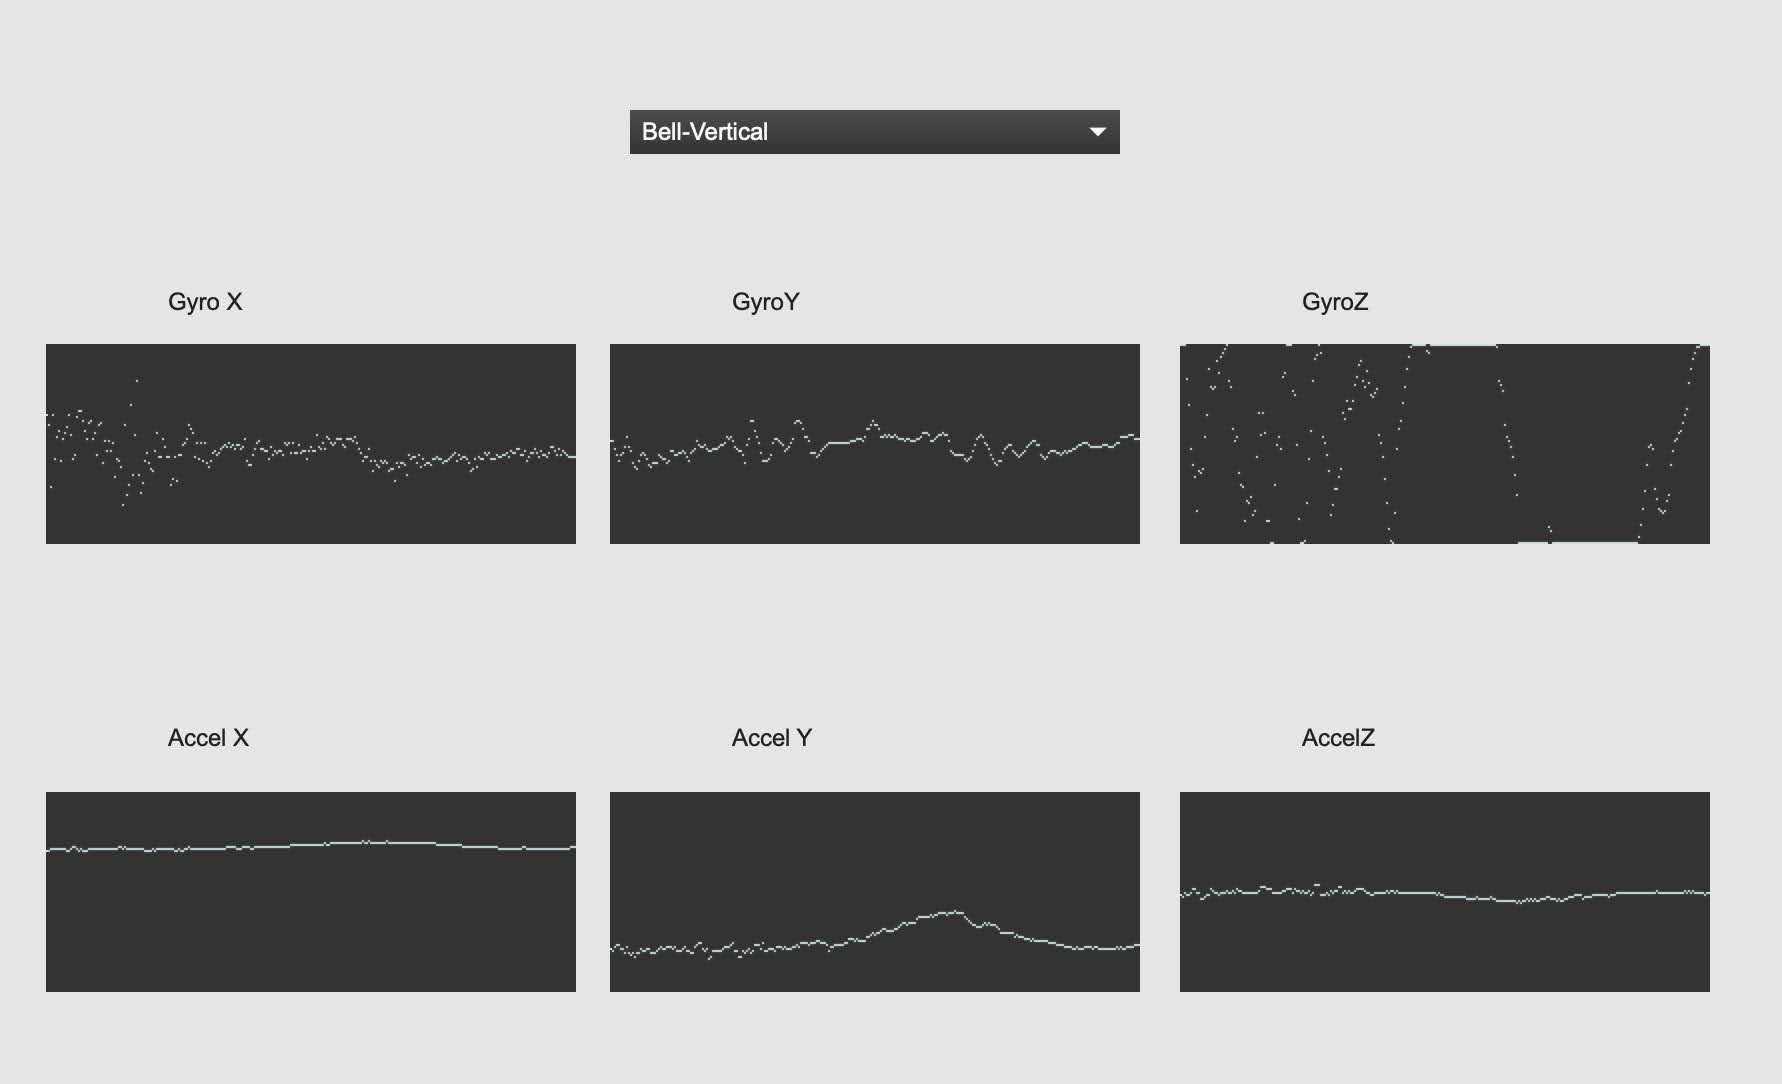
\includegraphics[scale=0.25]{diagrams/gestureData/bellVert.png}
    \caption{Raising the bell expressively.}
    \label{fig:bellRaiseData}
\end{figure}

When slowly raising the bell, a gentle slope can clearly be seen in the accelerometer's Y axis as one would expect. 

\begin{figure}
    \centering
    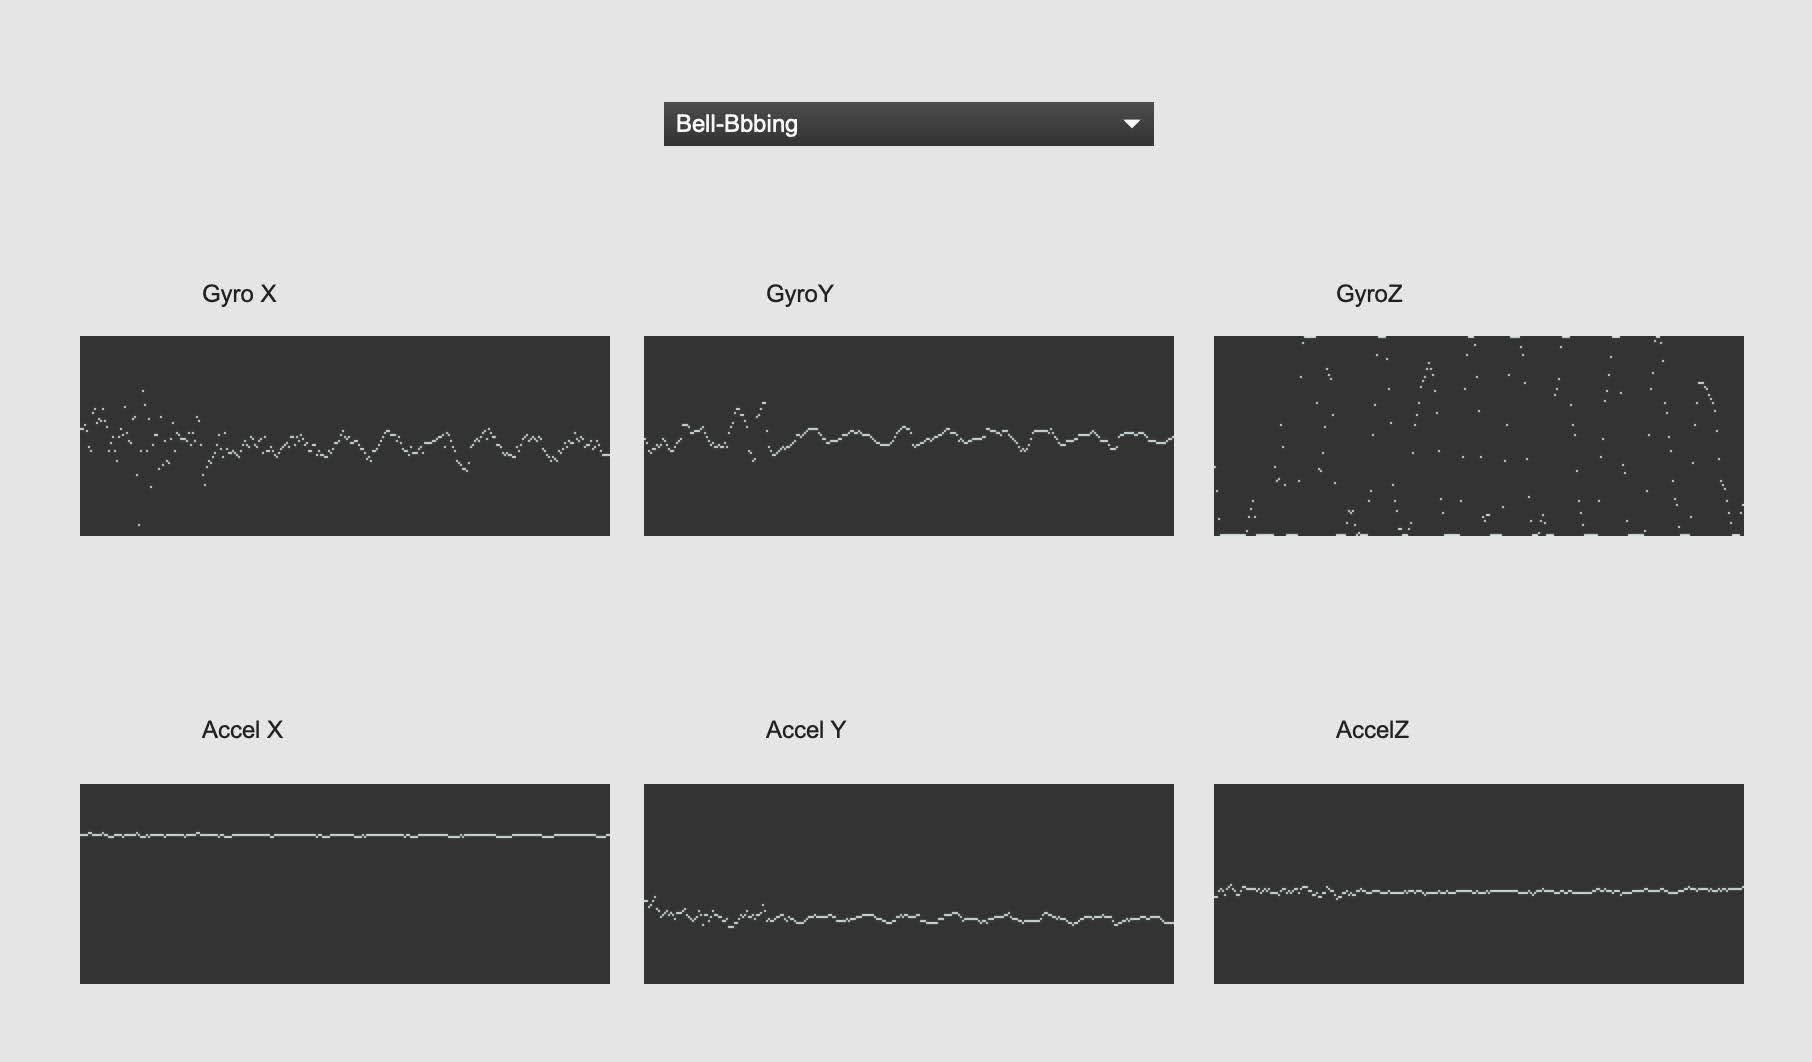
\includegraphics[scale=0.25]{diagrams/gestureData/bellBob.png}
    \caption{Small bobbing of the Cyberinet bell.}
    \label{fig:bellBobData}
\end{figure}

When bobbing the instrument bell, a clear bump appears in every sensor, similar, but smaller in scale to the single expressive raising of the horn shown in figure \ref{fig:bellRaiseData}. By focusing more on horizontal or vertical movements, different sensors will have larger slopes in their data. When testing, the vertical bell movement was approximately four-six inches. Larger bobs will result in larger data spikes.

Mathematically speaking, this relationship between movement size and speed can be easily calculated by working with the slope of the graphs. Taking into account any offset from the sensor's 0-point, moving a large distance or moving quickly will result in a grater change of data values. This general equation was created from reworking the equation of a slope of a line, wherein \textit{m} is equal to said slope. In practice, when repeating the same movement but highly exaggerated past a natural expressive limit, changes in data become more clear and useful when utilizing the data within Max. 

Air flow gestures have not been recorded in the same way as the movement gestures have. This is because breath control is intrinsically linked to the traditional Clarinet performance. As dynamics increase, the values also increase as more air is flowing through the instrument, and these gestures are already notated within a traditional score. 

\begin{figure}
    \centering
    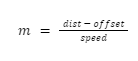
\includegraphics{slopeEqu.png}
    \caption{Equation for calculating slope of gesture graphs}
    \label{fig:mequSlope}
\end{figure}


\begin{figure}
    \centering
    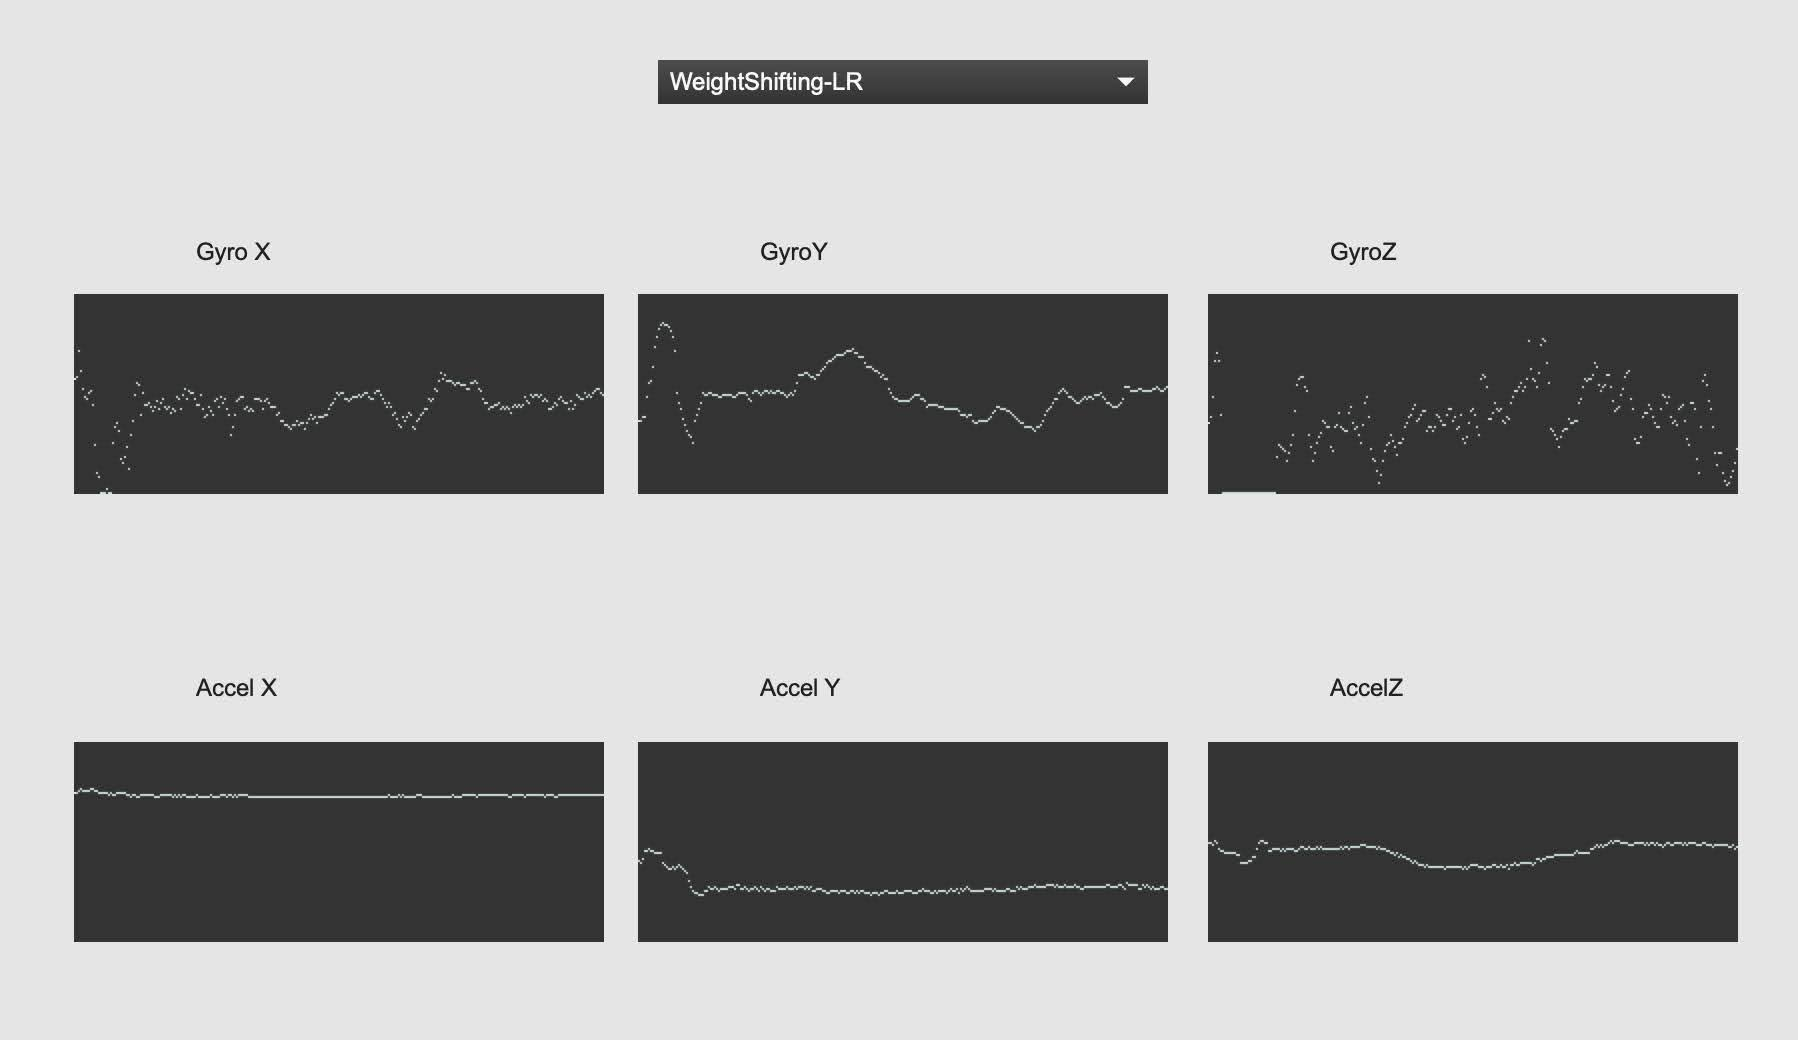
\includegraphics[scale=0.2]{diagrams/gestureData/weightshifting.png}
    \caption{Horizontal Movements in two directions.}
    \label{fig:exHor}
\end{figure}


 When looking at traditional gestures that occur naturally\cite{wanderleyClarinetGesture2005}, data changes are observed, but many of them are relatively static. This is to be expected as traditional Clarinet performance encourages limited movements and no rotations of the horn, so when attempting to adhere to traditional practice, the sensor data may prove relatively static. Figures \ref{fig:exHor} and \ref{fig:exVert} show this relationship. When performing the same movements, but exaggerated past the point of being a simple expressive movement, the range of data points in all sensors greatly increases. By utilizing exaggerated gestures as measured by Wanderley et al. or more experimental movements one can take more advantage of the Cyberinet's sensors.

 \begin{figure}
    \centering
    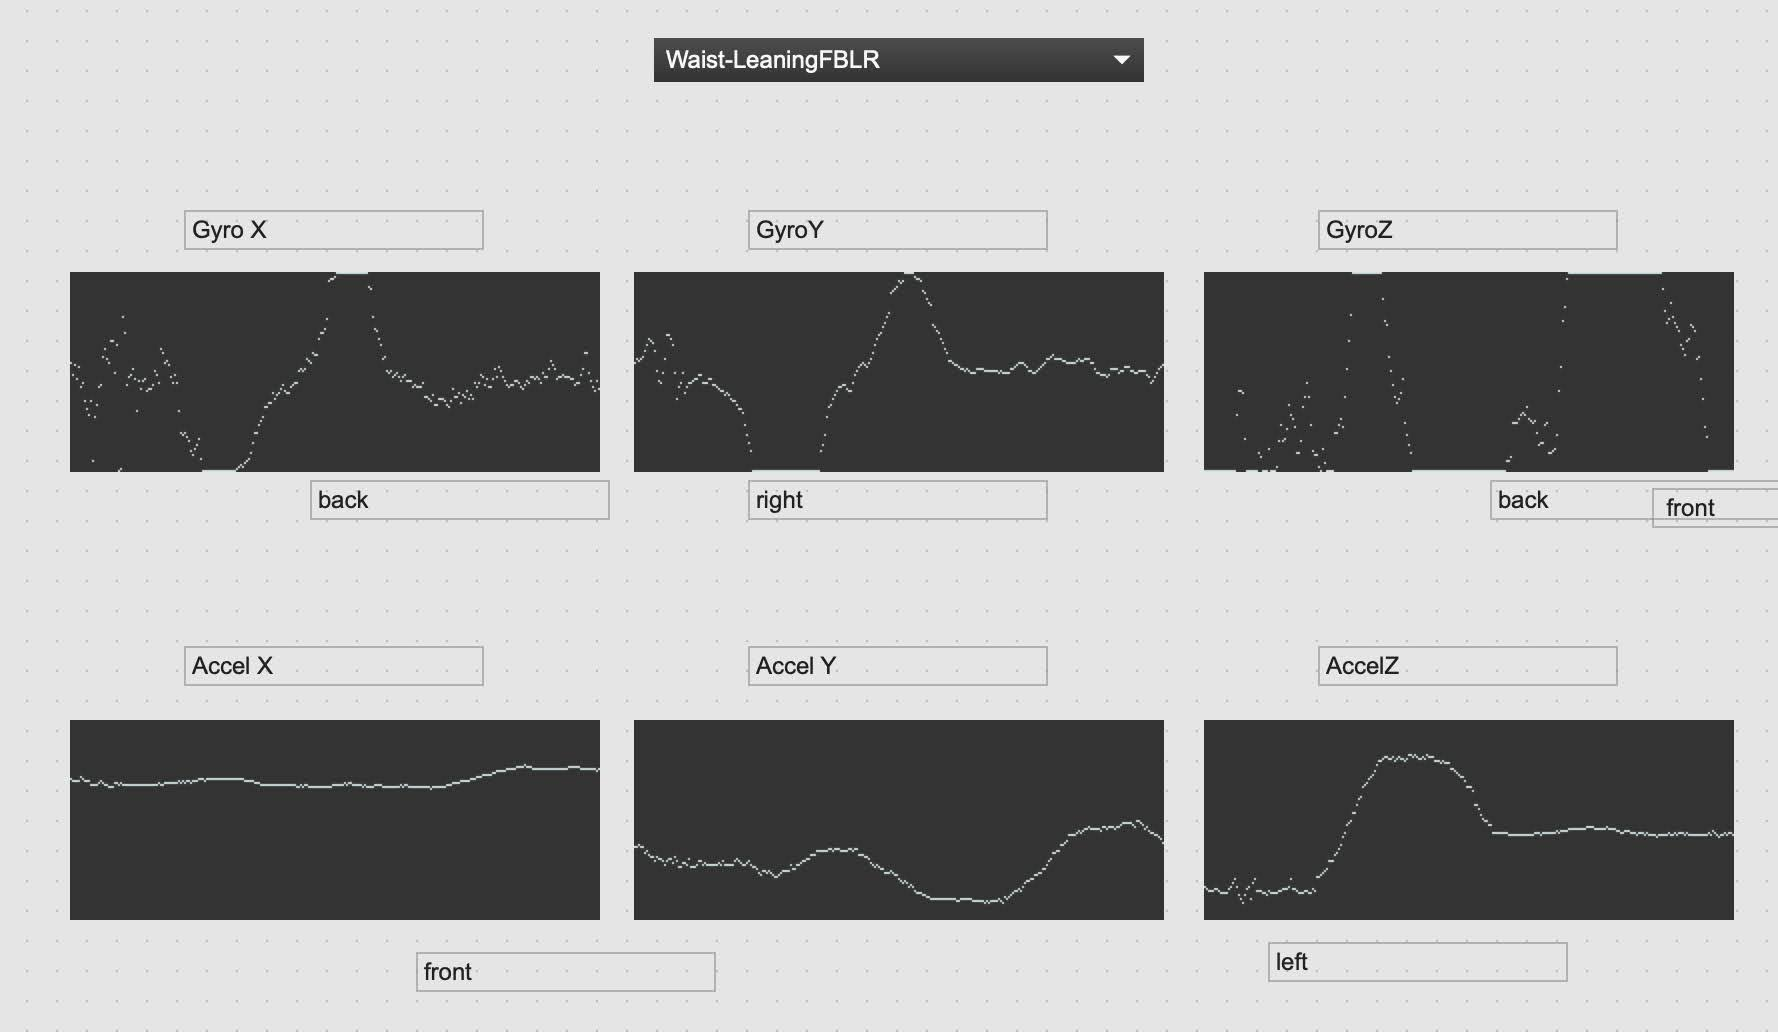
\includegraphics[scale=0.2]{diagrams/gestureData/waistLeaning.png}
    \caption{Exaggerated movements in four directions.}
    \label{fig:exVert}
\end{figure}

\begin{figure}
    \centering
    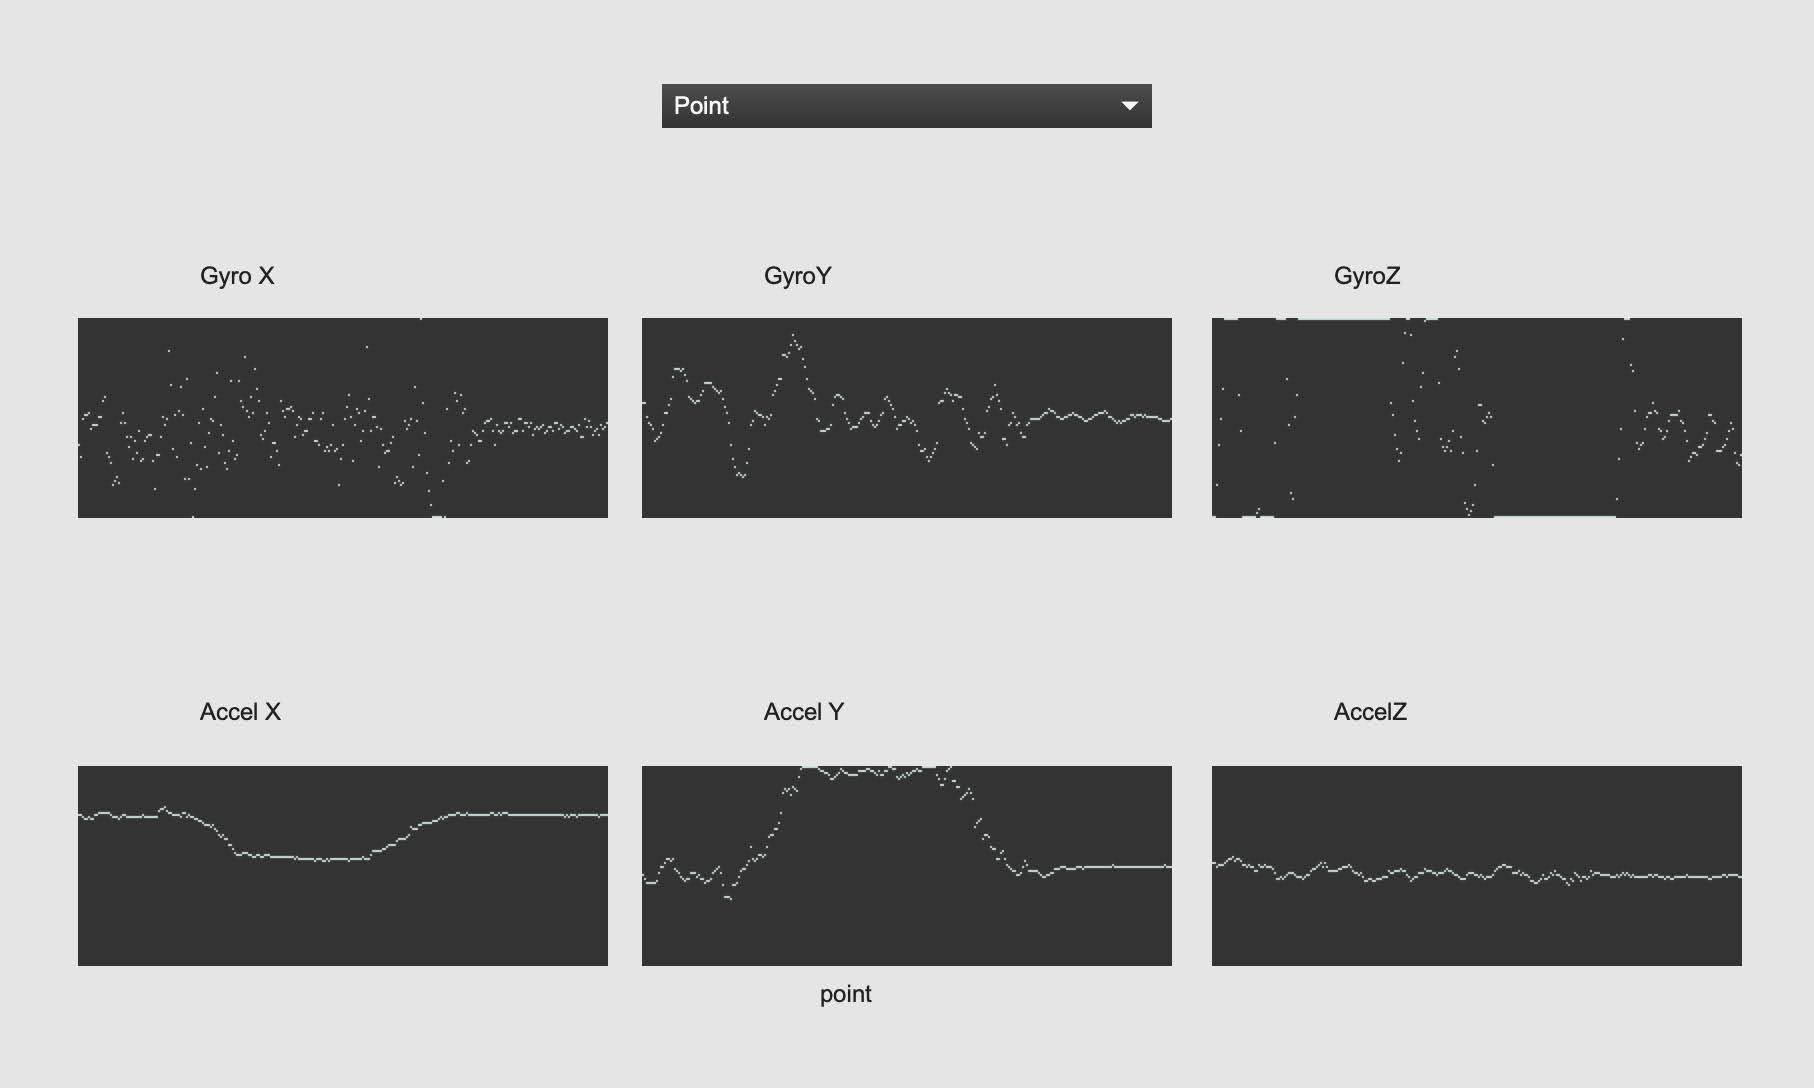
\includegraphics[scale=0.2]{diagrams/gestureData/pointing.png}
    \caption{Pointing the mouthpiece towards the audience.}
    \label{fig:pointData}
\end{figure}

For the gesture shown in figure \ref{fig:pointData}, the mouthpiece was removed from the mouth and pointed forward towards the audience, then returned to playing position. The most clear showing of this has been highlighted, and shows a clear beginning and end to the gesture. Figure \ref{fig:clotRotate} shows data from holding the instrument at arm's length and rotating it 360 degrees in a circle. The high values in the gyroscopic Y-axis show the direction, while all of the accelerometer data moves down and back as the horn passed 180 degrees and began to return to the initial positioning.

\begin{figure}
    \centering
    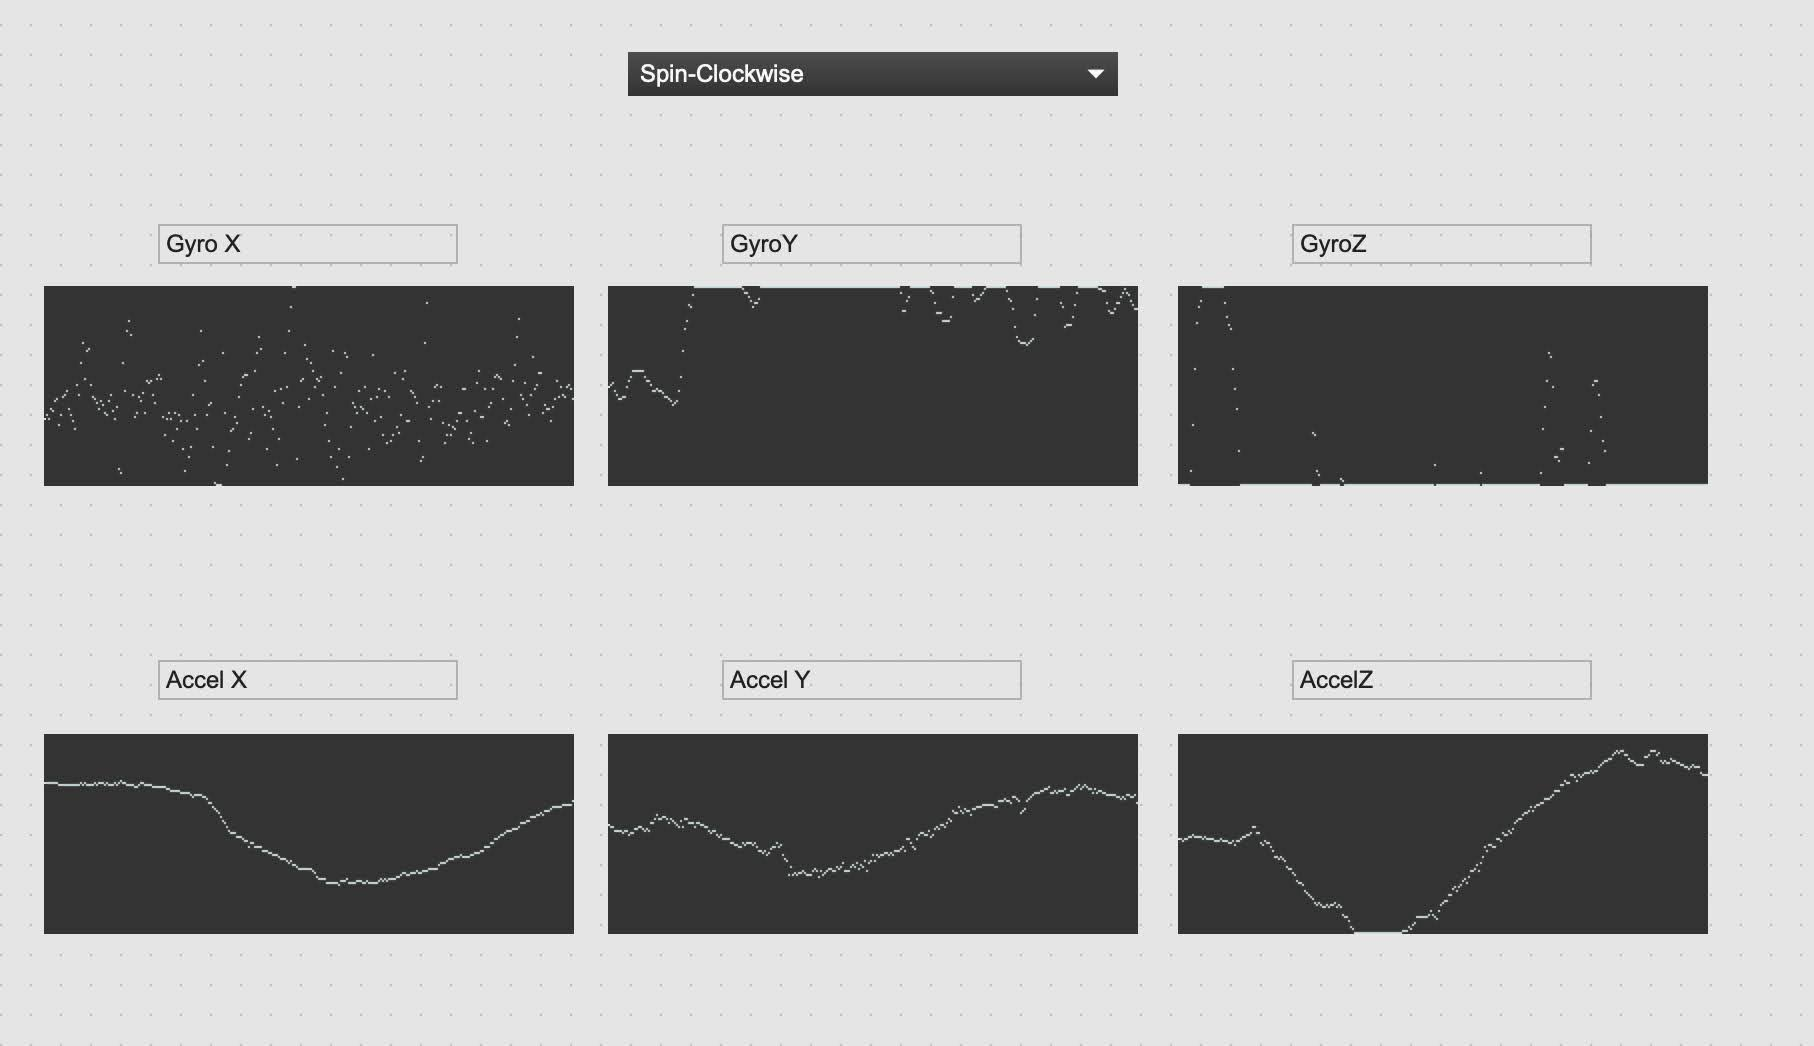
\includegraphics[scale=0.2]{diagrams/gestureData/spin Clockwise.png}
    \caption{Clockwise Rotation of the Cyberinet.}
    \label{fig:clotRotate}
\end{figure}

When flicking the Cyberinet, it is held vertically and quickly rotated either left or right, then returned to center. This results in a quick, high peak in the sensors\footnote{The exaggerated nature of the gyroscopic Z values can also be seen in figure \ref{fig:clotRotate}, but this relationship is clearer in the other visualizations}. In the case of these more experimental gestures, all of these are not an action one would expect to see in traditional Clarinet performance. By comparing the data from a gesture to the intended mapping within Max, the composer can determine the most effective mappings. Gestures with a higher slope when viewed through CNET.gestureVisualizer are generally appropriate for actions such as gates and triggers within the software environment. Slower gestures are useful for creating perceptible changes over time. A composer can also choreograph specific gestures in order to create a specific shape to the data for use within the software.

\begin{figure}
    \centering
    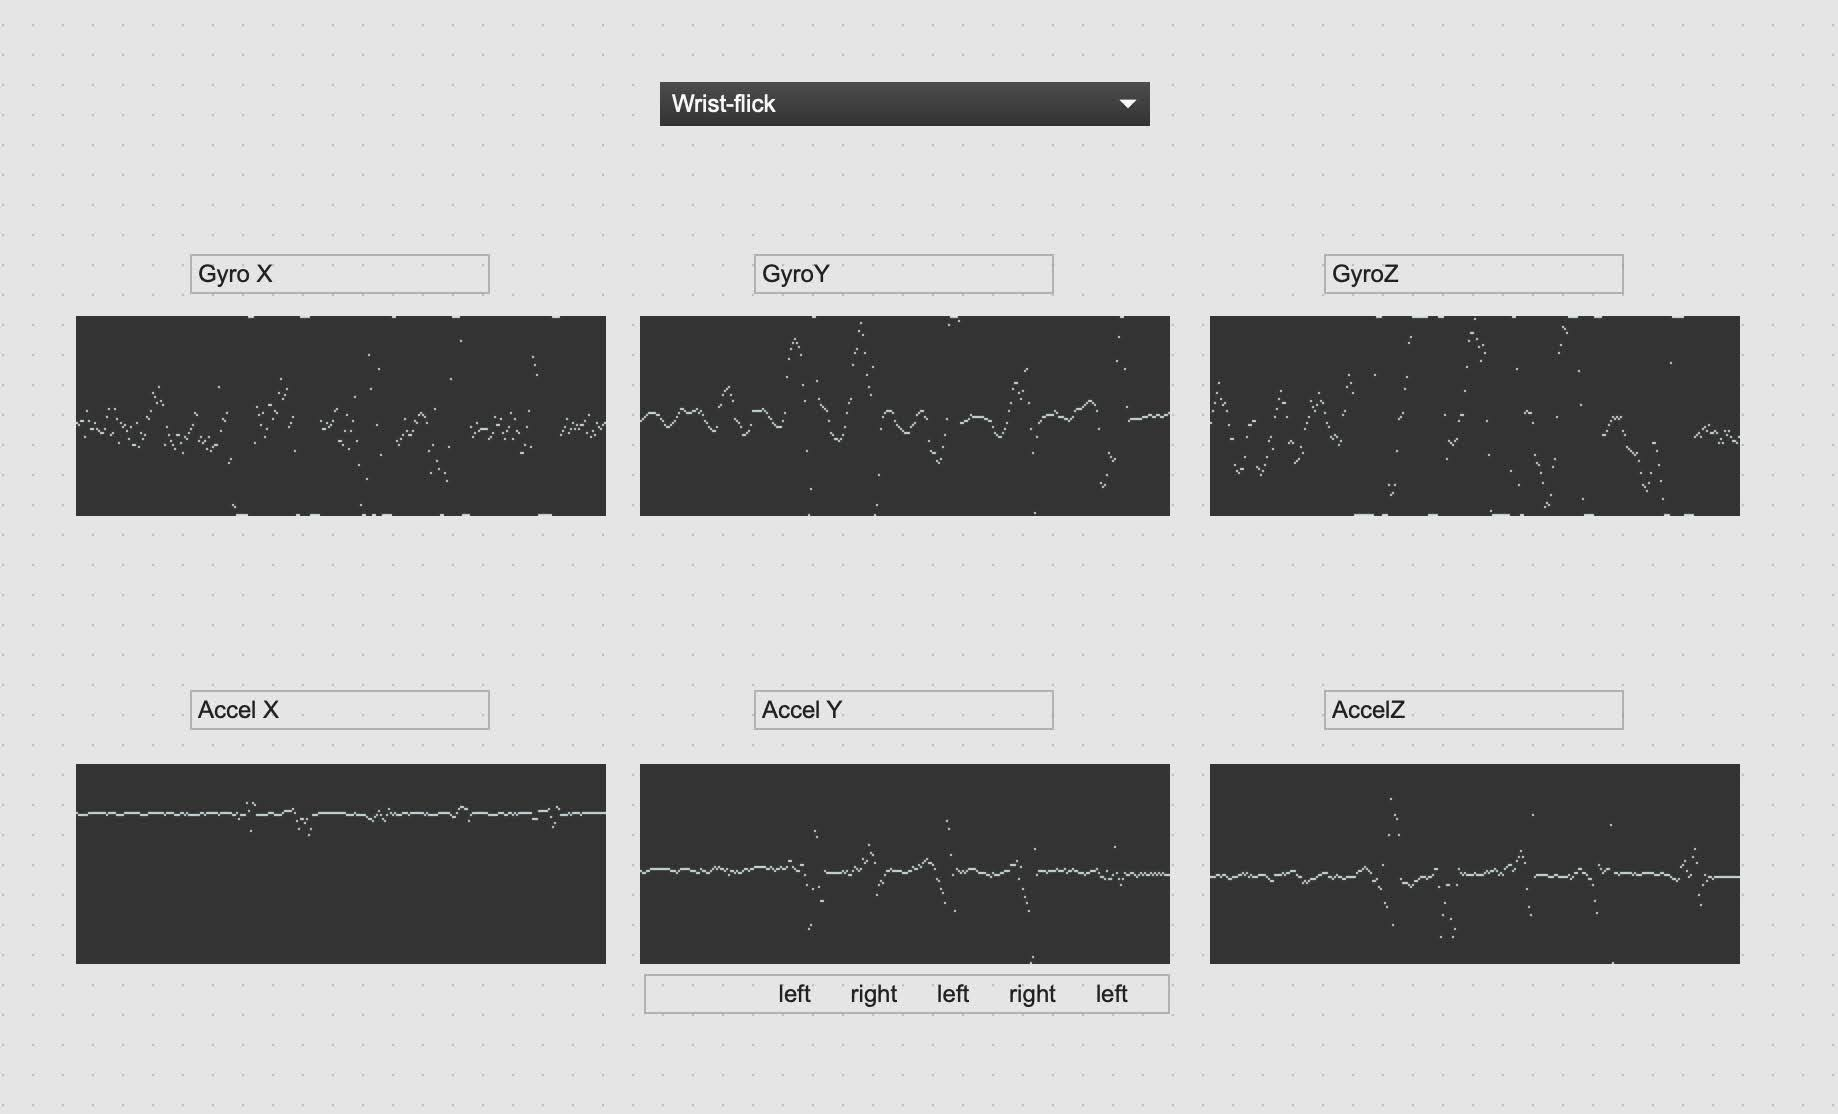
\includegraphics[scale=0.2]{diagrams/gestureData/wristFlick.png}
    \caption{Flicking the wrist while holding the Cyberinet.}
    \label{fig:cflick}
\end{figure}

\subsection{Sound Synthesis}

The Cyberinet does not directly generate sound outside of those produced by the base Clarinet. Because of this, the software takes the sensor data, represents it as a number, then utilizes those numbers within the Max programming environment. A handful of Max objects have been created to help facilitate this feature, and for new users to quickly implement the Cyberinet without the need to be an expert in Digital Signal Processing (DSP) and audio effect programming.

All of these effects are built in Max and utilize common control parameters. With the exception of any signal input, receive sensor data as floating point numbers between 0 and 1. If the user would like their physical gestures to generate a sound, those data points must be routed to an object which creates sound within Max.
 

\subsection{Feedback Mechanisms}
If following along with the order presented by Miranda \& Wanderley in table \ref{tab:generalGestures}, Step 4 has already been discussed. Skipping ahead to Step 5 sees the creation of feedback mechanisms. These proved surprisingly difficult to determine in initial planning and prototyping. Ultimately, two main methods were decided upon to be useful for both the performer and someone working in the Max environment, without being distracting. On the physical unit are multiple LED's. Several of these are used to indicate that the sensors are properly functioning, but one LED can be programmed to have a specific functionality. 

At the moment, version 1.3 of the software is utilizing the programmable LED to indicate when the sensor data transmits to the computer. This proves useful for determining whether a connection with the computer is established, and if data should be expected by the computer. In order to avoid blinding the user with LED's they are hidden behind the hardware case of the Cyberinet, and small holes are included to allow for intentional inspection, Similar to the metal grates on microwave doors to allow the user to look in on the food while avoiding the microwave radiation. This programmable LED is located close to the airflow sensor's tubes, allowing for the airflow tube to also function like a fiber optic cable so that the information can be easily read without needing close internal inspection through the aforementioned holes.

\begin{figure}
    \centering
    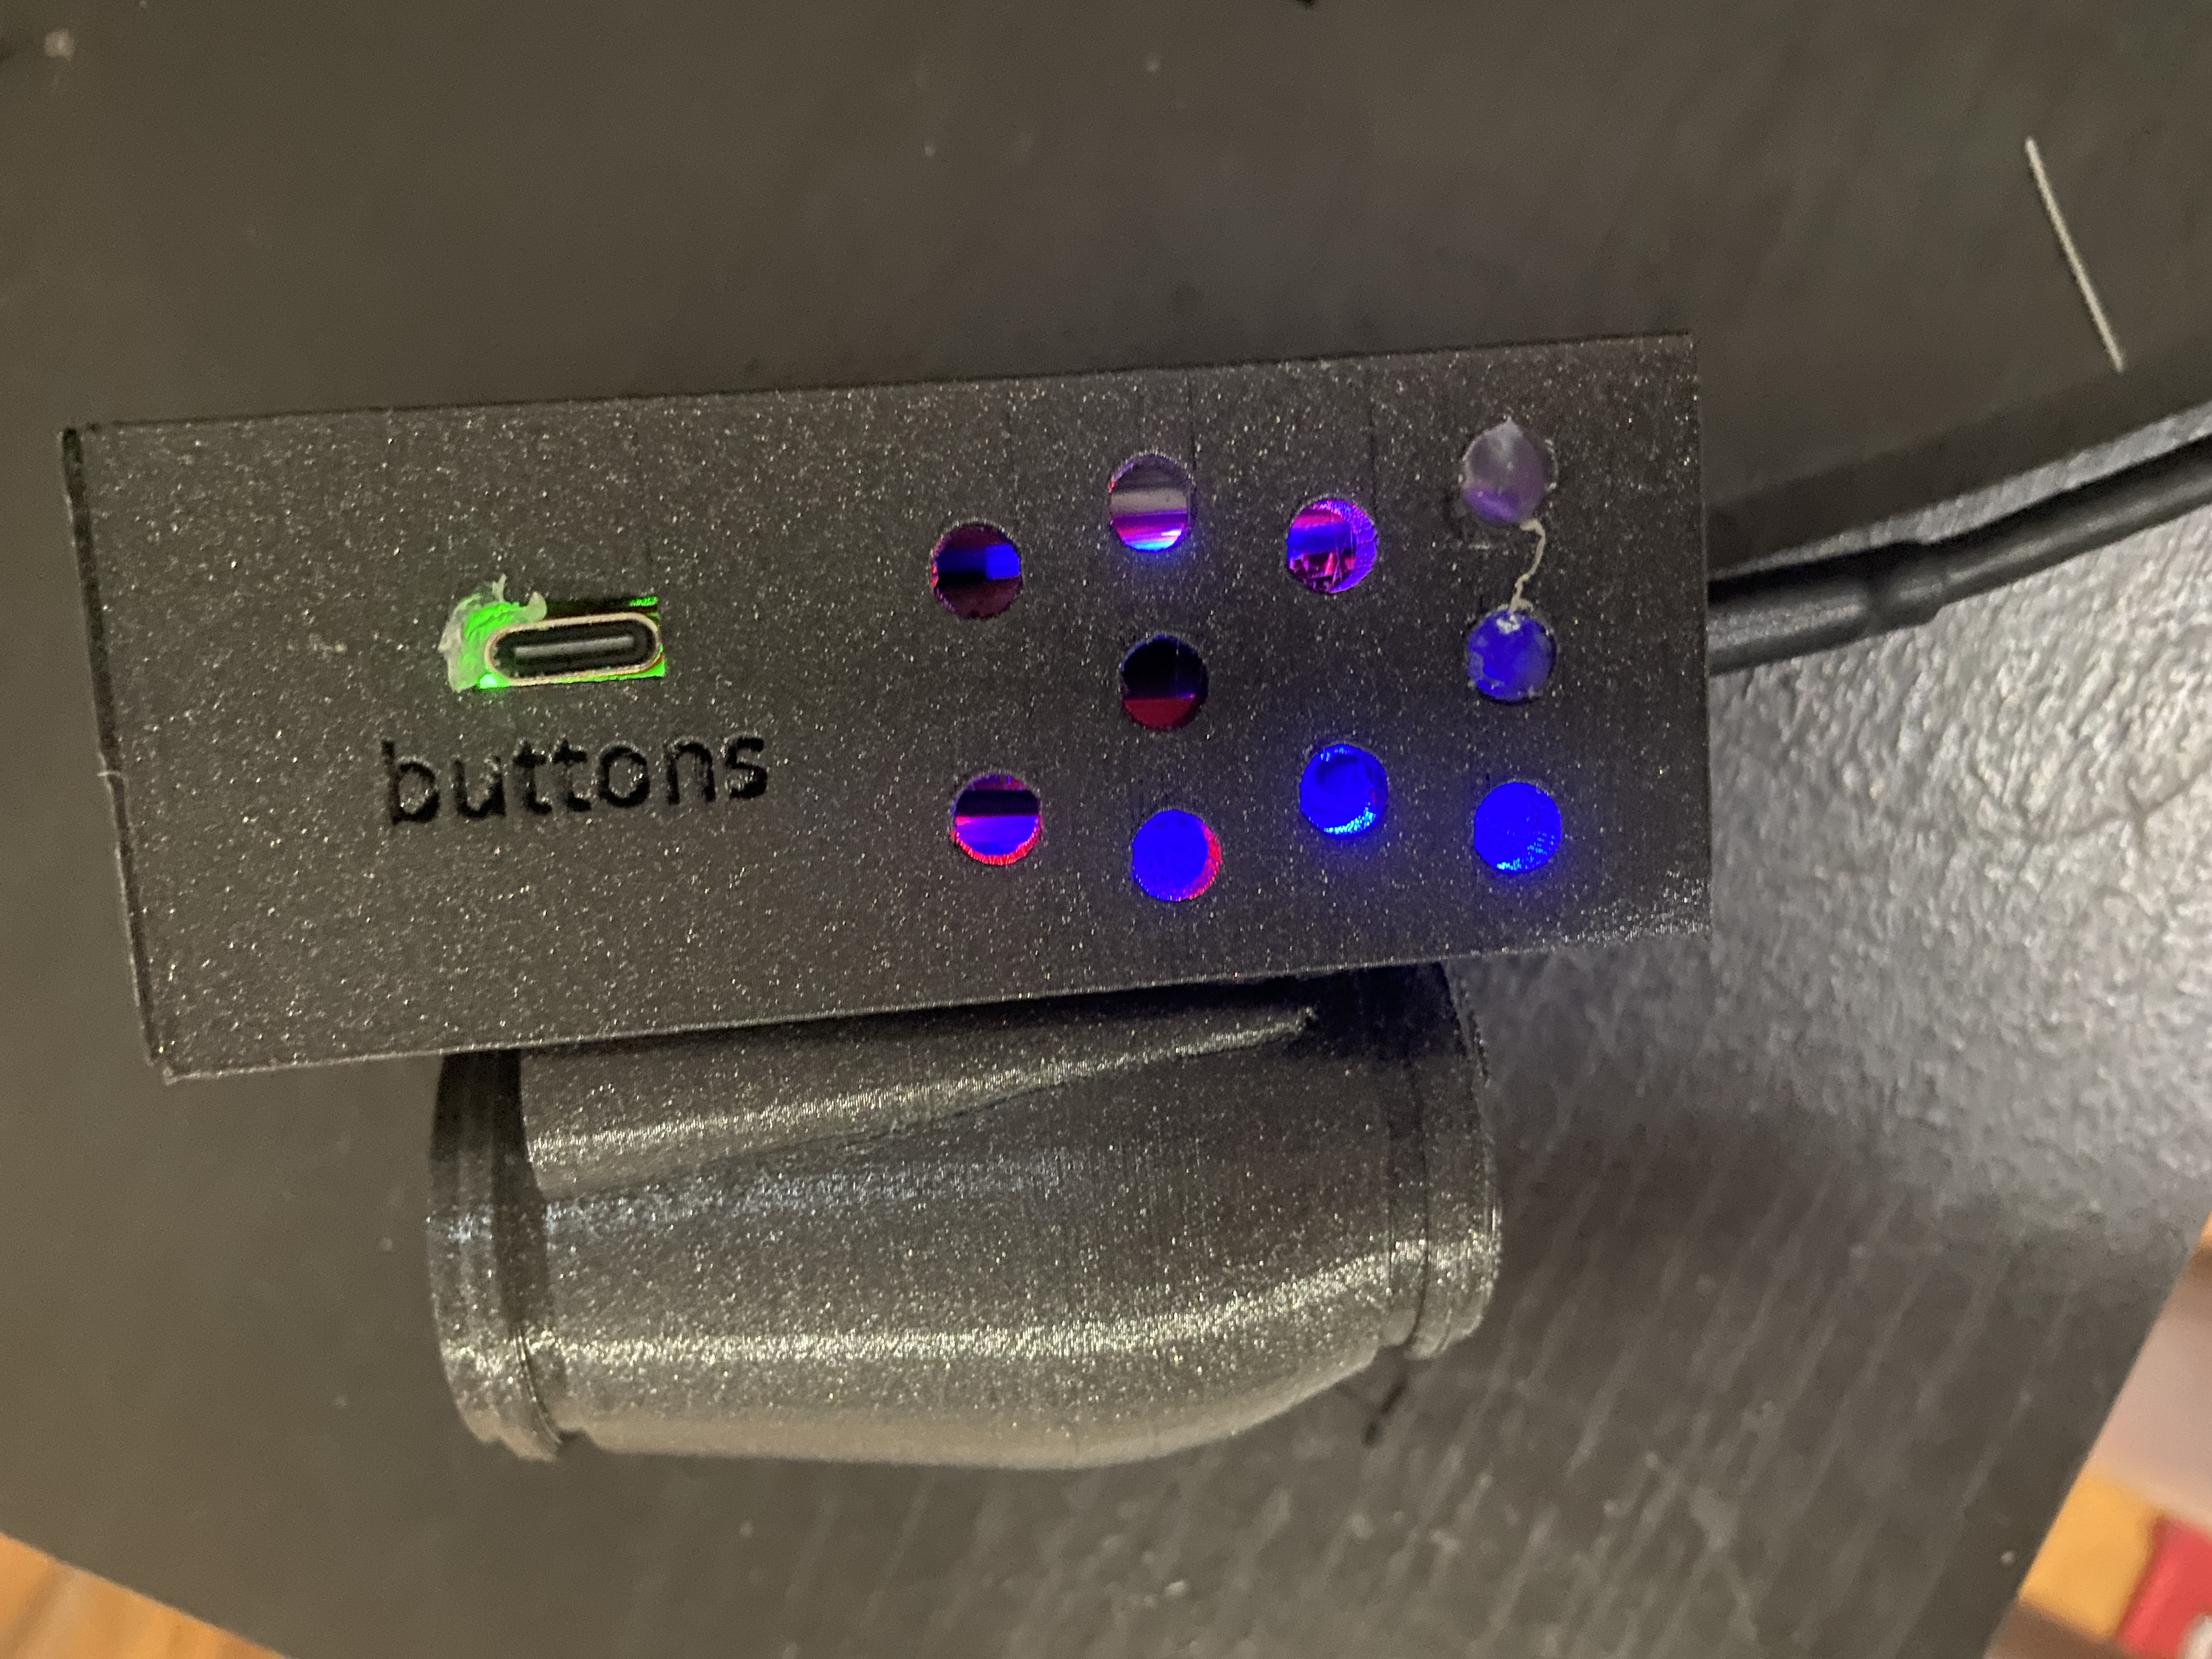
\includegraphics[scale=0.05]{diagrams/IMG_2210.JPG}
    \caption{Power/charging indicator LEDs on the Cyberinet main unit.}
    \label{fig:CyberinetLEDs}
\end{figure}

\begin{figure}
    \centering
    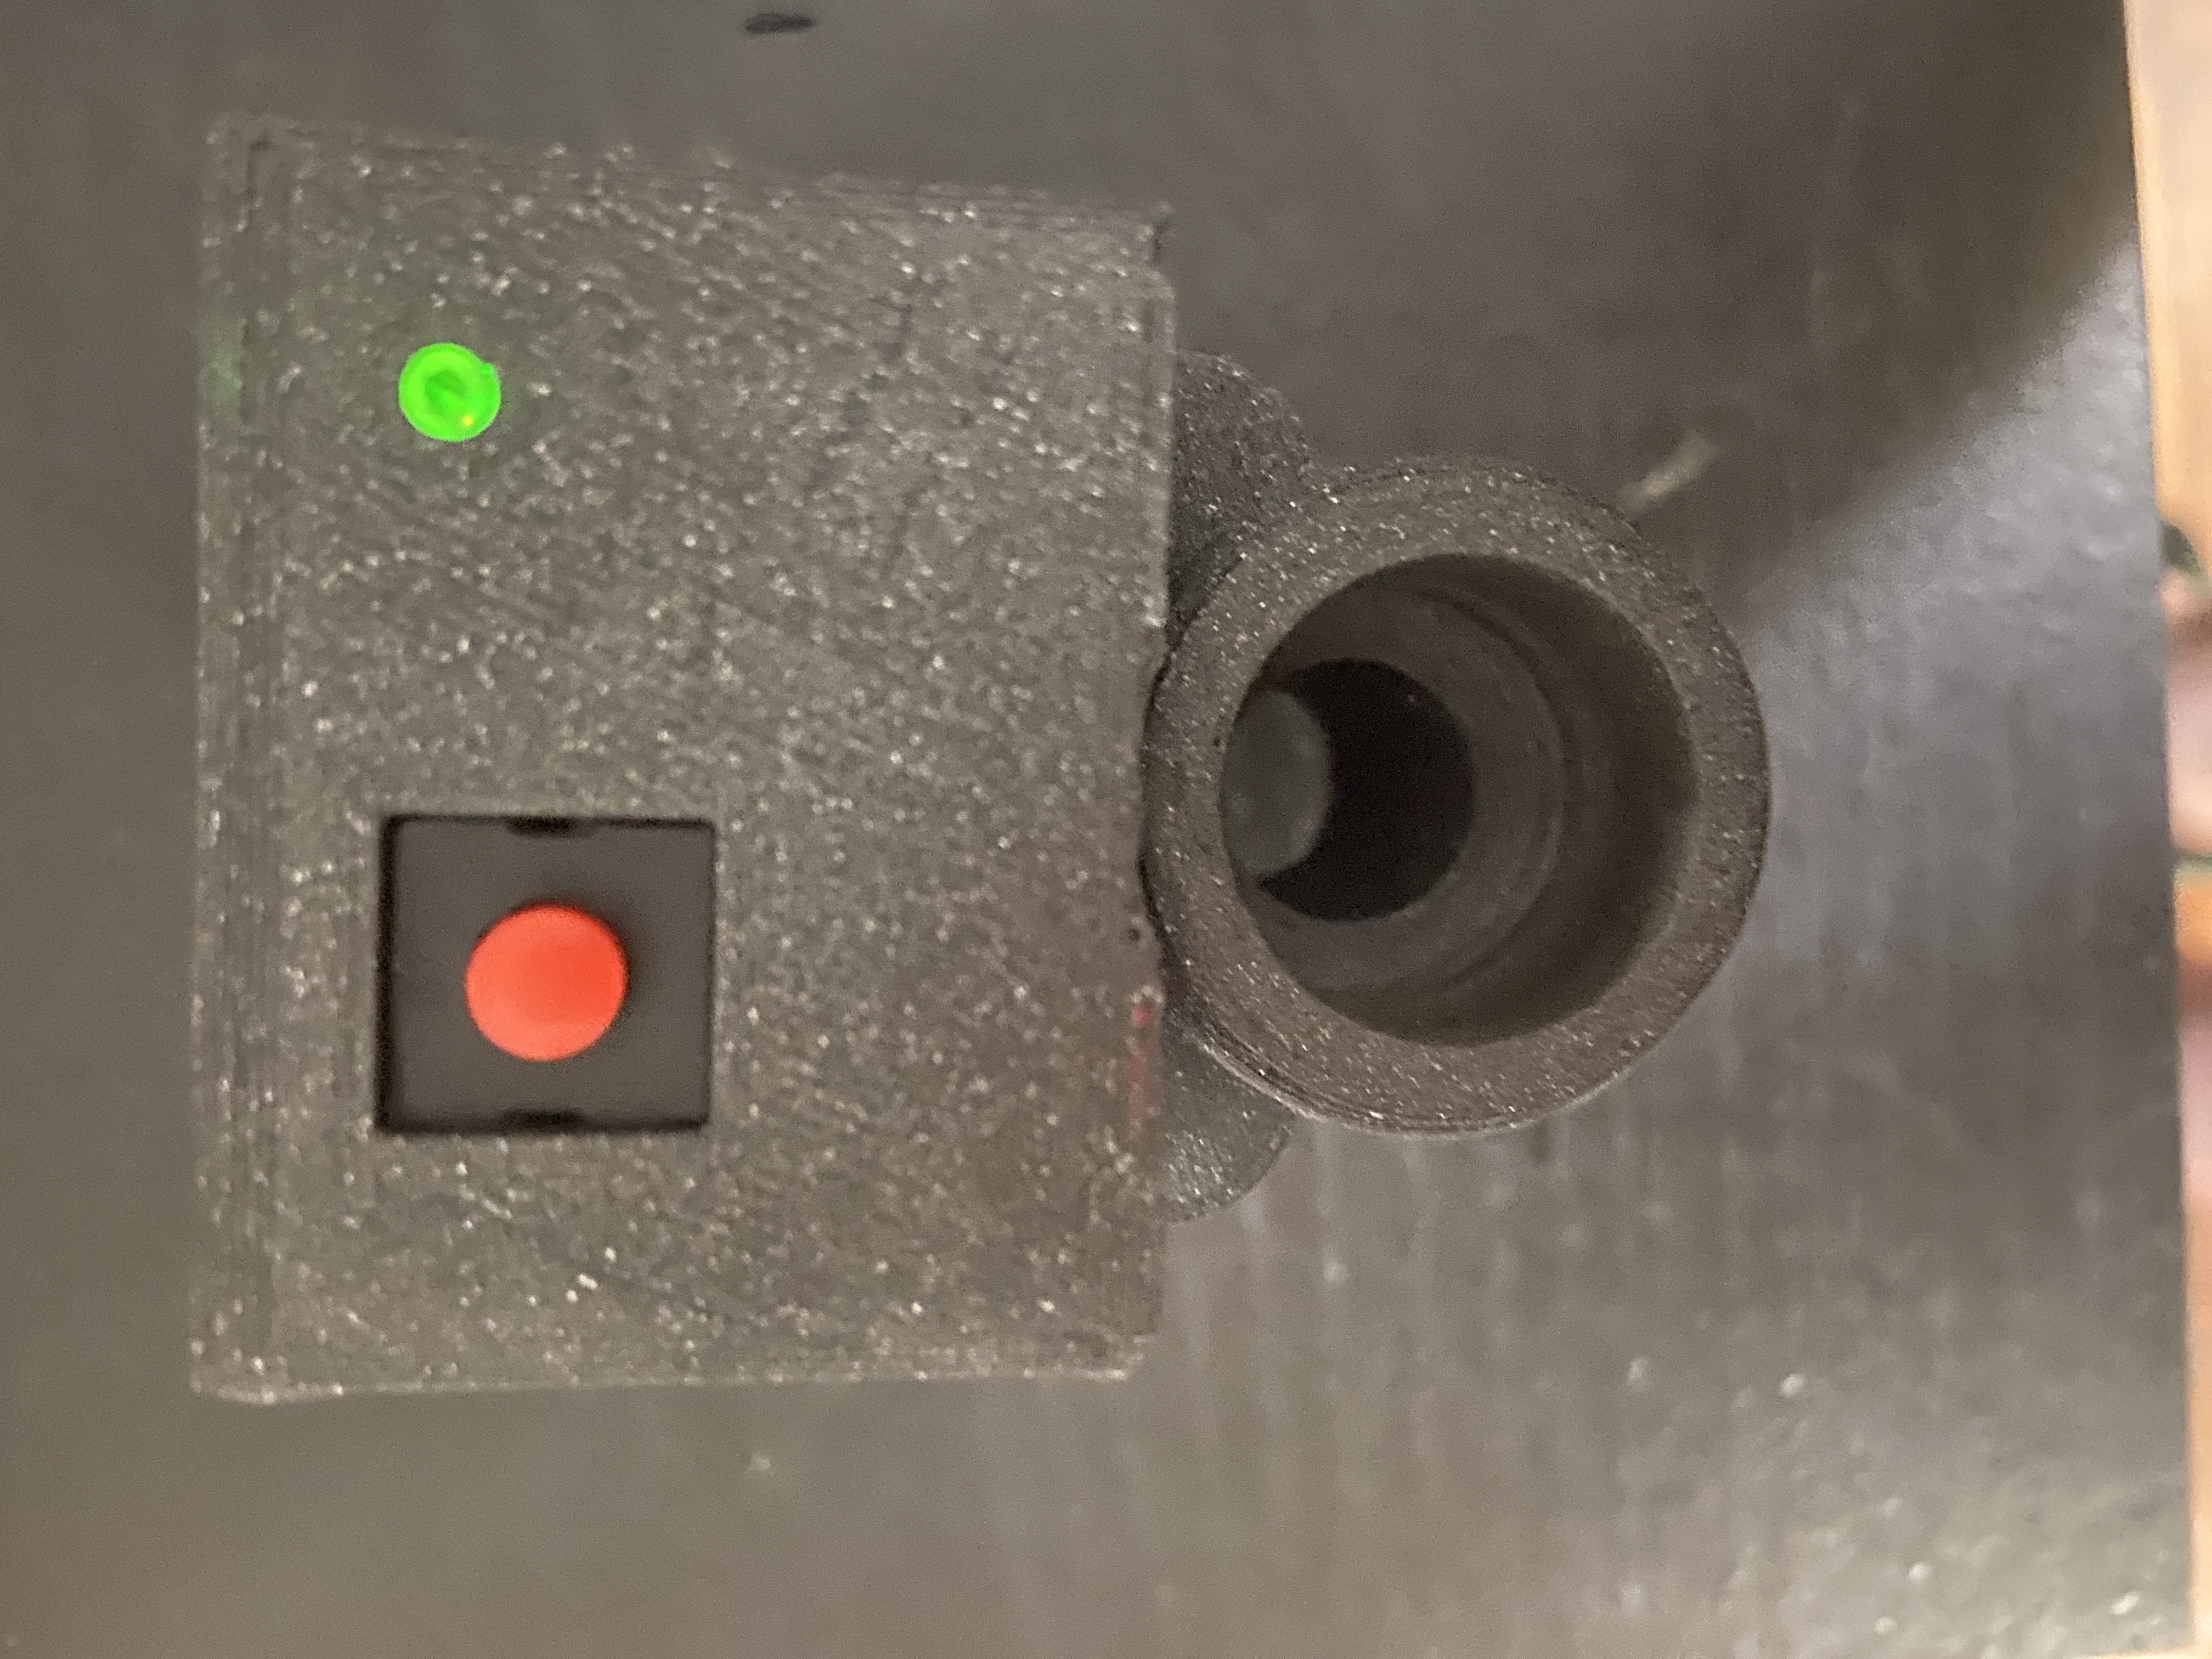
\includegraphics[scale=0.05]{diagrams/IMG_2211.JPG}
    \caption{Toggleable LED visible to the performer while performing.}
    \label{fig:msgLED}
\end{figure}


In the software, a handful of options are available to provide feedback in regards the incoming data and any errors. If an unrecognized sensor reading or control message is received by the core CNET software object, this is returned to the user via both the final outlet of the object, as well as the Max console. Because a user would have to go out of there way to include monitoring within the patch, the main Cyberinet patch is able to display all incoming data in the Max console, as well as indicate when communication begins and ends. This is useful for monitoring and recording the incoming data, as well as being able to identify any errors from the sensors or control messages.


\section{OEM Components}

OEM products are designed to generally compatible with each other. The acronym stands for Original Equipment Manufacturer, and these manufacturers create parts that can be utilized in a variety of different products due to said compatibility. In the case of the Cyberinet, all of the components utilize standardized 0.1in spacing between each pin as well as a common voltage to power the sensor at 3.3V. Every part in the Cyberinet is compatible with these OEM standards, and this is the key to the future expansion units.

While testing various OEM sensors and their capabilities in a performance setting, a series of prototype boards were developed. Early prototyping was done on a bread board in order to test specific uses of pins on the micro-controller and combinations of different sensors. The second step involved creating a hand-soldered board using sockets to be able to easily add or remove components. Once the desired pins and sensors were determined, the socket boards were translated into a more condensed PCB. These were initially created with sockets to allow for more testing and prototyping for future revisions. Once the final design was decided, components were directly soldered to the PCB for formal data capture testing and performance use.

The choice to utilize OEM sensors for the seminal version of the Cyberinet arose both from the outlined method of prototyping, and in order to keep the overall cost down. One of the main design intentions of the Cyberinet was a relatively affordable price point. 

\begin{figure}
    \centering
    \includegraphics[scale=0.55]{diagrams/builtUnits/protos.png}
    \caption{Early prototype socket boards}
    \label{fig:protoBoard}
\end{figure}



\subsection{Micro-Controller \& Power Distribution}

The Cyberinet contains a variety of useful sensors, however without the micro-controller, they become effectively useless in this context. In order to effectively manage all of the sensors and transmit the data, the Espressif ESP-32 DEVKIT V1 was ultimately selected for use with the Cyberinet. This board was selected for a handful of reasons, including:

\begin{itemize}
    \item Board's narrow size
    \item Large number of ports
    \item Arduino compatibility
    \item Wireless communications
\end{itemize}

The first two items on this list are closely related. While being narrower that comparable Arduino units such as the Uno, the ESP-32 DEVKIT V1 also has 30 unique I/O Pins\footnote{Other versions of the DEVKIT have 36 GPIO pins. \\These boards are incompatible with the PCBs used in the Cyberinet.}. There are Arduino boards with similar features, but they were either too large or cost prohibitive to the final design. While four pins on the ESP-32 are dedicated to power distribution and another for the 'enable' functionality (EN) and resetting the board, the remaining pins be utilized for sensors in a variety of ways. All of this potential functionality is compressed to just under three centimeters wide, resulting in a large amount of potential uses within a smaller footprint. 

Because of the semi-modular design of the Cyberinet unit, having a large amount of accessible pins in a smaller unit was considered ideal. The DEVKIT V1 was preferred over the significantly smaller base chip to increase the simplicity of prototyping, repair, and future changes due to its OEM compatibility, and the popularity of the board among the community. For clarification, the ESP-32 is only the chip encased in a metallic heat sink in figure \ref{fig:protoBoard2.1}, whereas the DEVKIT consists of the larger black unit as a whole.

\begin{figure}
    \centering
    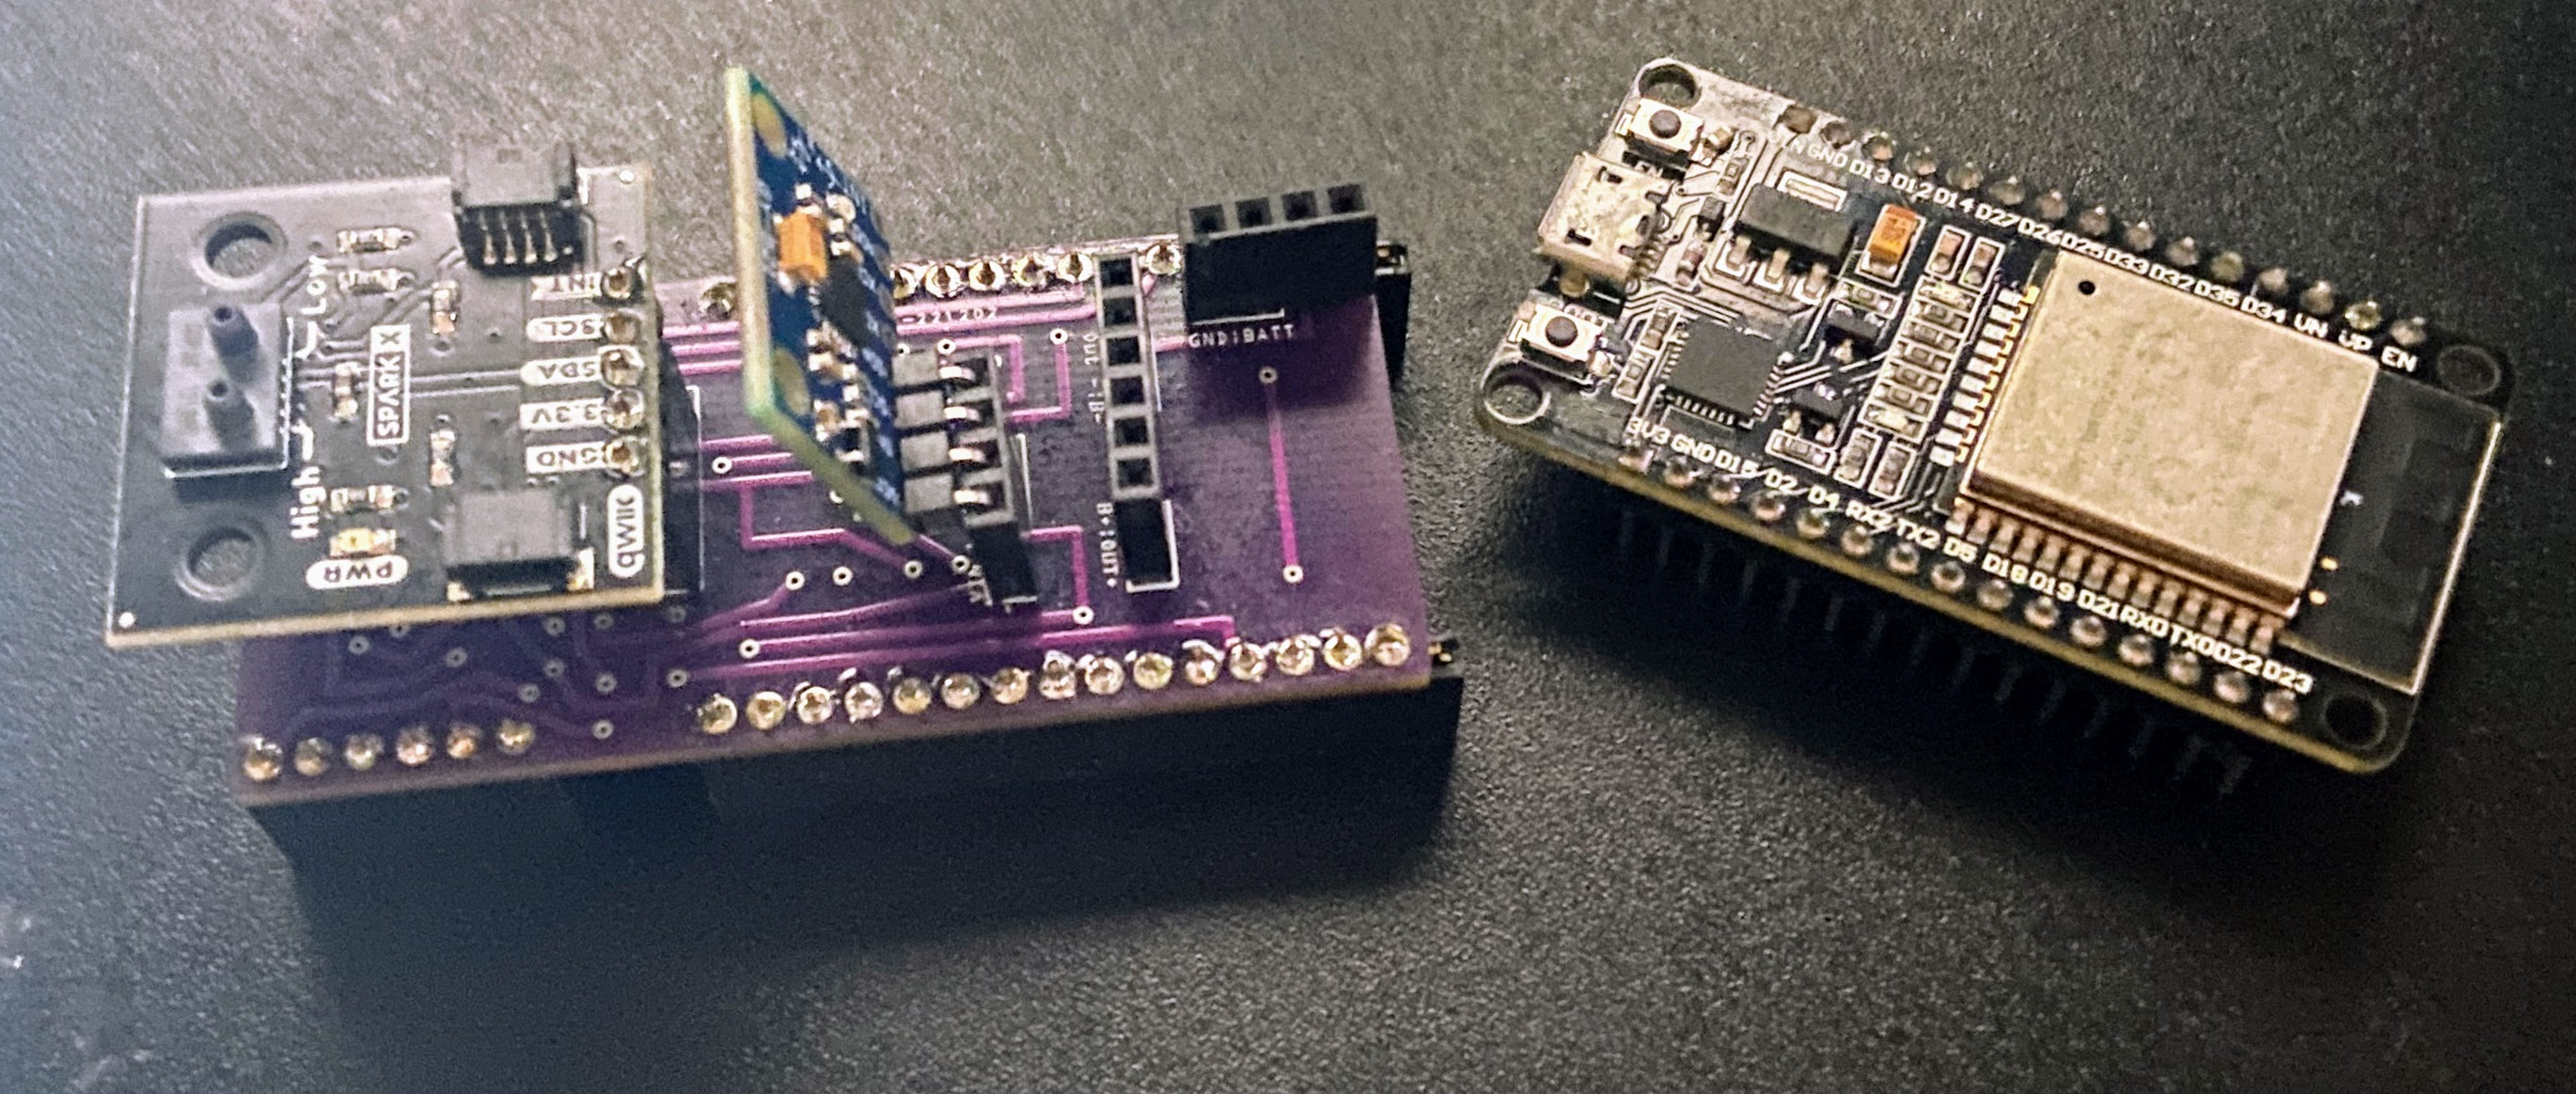
\includegraphics[scale=0.15]{diagrams/builtUnits/protoBoard.JPG}
    \caption{ESP-32 shown next to a prototype PCB. (reprint)}
    \label{fig:protoBoard2.1}
\end{figure}

 

Because of the large number of Pulse-Width-Modulation-Controlled GPIO pins, the Cyberinet has the potential for a large number of sensors and expansions, but to help contain the form factor, only a handful are being utilized at any time. We can see the included sensors attached to the pins as shown below. The labels in the figure below utilizes the pin labels that are printed on the DEKVIT V1.

\begin{table}[]
    \centering
    \begin{tabular}{|c||c|}
    \hline
    Pin Label & Connection\\
    \hline
    \hline
    Vin     & Power from battery \\
     \hline
    GND     & Ground \\
     \hline
    2       & Power Indicator LED \\
     \hline
    4       & Programmable LED \\
     \hline
    12      & Button 1 \\
     \hline
    14      & Button 2 \\
     \hline
    18      & Expansion return pin 4 \\
    \hline
    21      & MPU6050/SDP31 Data \\
     \hline
    22      & MPU6050/SDP11 Clock \\
    \hline
    26      & Button 1 LED \\
    \hline
    27      & Button 2 LED \\
    \hline
    32      & Expansion return pin 1 \\
    \hline
    33      & Expansion return pin 2 \\
    \hline
    35      & Expansion return pin 3 \\
    \hline
    \end{tabular}
    \caption{Main Unit Core pins}
    \label{tab:mainPins}
\end{table}

The code written for the ESP-32 DEVKIT was created using the Arduino IDE and coding language. For similar reasons to the choice of the DEVKIT, this was done for greater accessibility and simplicity in programming. The board is capable of being programmed in a variety of languages depending on the intended use and the programming abilities of the user\footnote{Compatible languages include variations on JavaScript, Python, C++, and other propritary languages developed by Espressif.}. 

The final item from the initial list of board necessities was the wireless capabilities. The ESP-32 is able to perform serial communications with a connected computer via a micro-USB or USB-C cable (depending on the board version). While useful, the goal of the Cyberinet is to provide affordable instrument augmentation with minimal alterations to the Clarinetist's performance practice. Towards this goal, minimizing the number of extra cables was a design concern from the first prototypes. By utilizing the ESP-32's built-in Bluetooth capabilities, the performer is able wirelessly communicate with the computer utilizing the same serial protocols.

The ESP-32 also has WiFi connectivity capabilities which may be involved in a future version, but at the current time is currently not utilized. The DEVKIT is able to support Bluetooth version 4.2 and Low Energy protocols for local wireless communication. This allows for the Cyberinet to pair with any computer that it has previously connected to using the Bluetooth Serial Arduino library. A code library created by Espressif that brings the normal wired Serial functionality to the Bluetooth functionality of the ESP-32. While not as powerful as the most up-to-date Bluetooth hardware, the DEVKIT's version 4.2 allows the Cyberinet to connect to a computer from up to 200 feet away with a max data transfer speed of 1 Mbps\cite{btSpecs}. While these values do fluctuate depending on the performance venue layout, and have a minor impedance from the case of the Cyberinet itself, the performance statistics are still high enough for a large majority or performance areas.

\subsubsection{Power Distribution}
In order to power the entire system, a lithium ion polymer battery is included inside the hardware. In order to charge the unit, users can utilize the provided USB-C cable and power adapter to the port located on the bottom of the unit. All power distribution for the Cyberinet is handled with a TP-4056 chip, shown in figure \ref{fig:tp5046}. The version containing a USB-C connector was chosen over the Micro-USB connector because of a desire for consistent, modern connectors in the device, which was justified by the board being identical with the exception of the type of port utilized. This chip helps to prevent overcharging and other power regulation of current within the system.


\begin{center}
    \begin{figure}
        \centering
        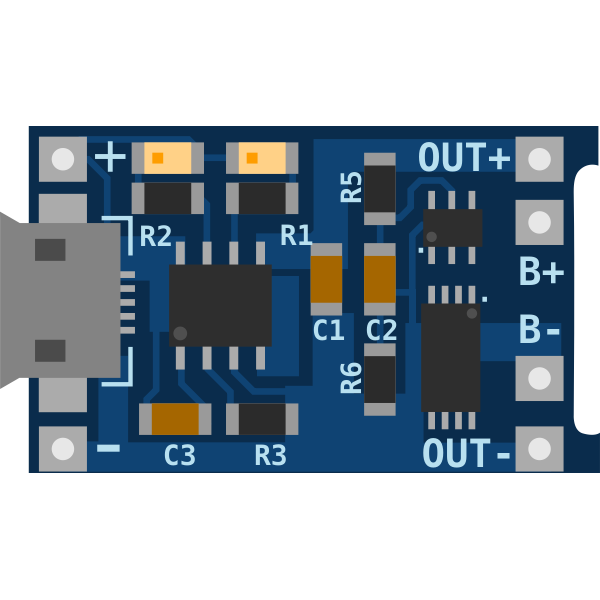
\includegraphics[scale=0.3]{diagrams/1554633962.png}
        \caption{Mock-up of the TP-4056 Power Distribution Chip used in the Cyberinet,\\used by permission}
        \label{fig:tp5046} % public domain svg
    \end{figure}
\end{center}

By connecting the battery to the connections labeled B+ and B-, and connecting the Vin and GND pins of the ESP-32 to the OUT+ and OUT- on this board respectively, the Cyberinet is able to receive all required power through this single chip. The power button is soldered into the connection between the battery ground and the TP-4056, and will automatically power the Cyberinet when activated. Because of the placement of the power switch, the device must be powered on while charging. This can be easily verified by the onboard LED's. The button is located on the top of the unit, allowing for easy access. The specific placement is shown in figure \ref{fig:msgLED}. 

When the battery is depleted, it must be connected to a power source via the USB-C port on the bottom of the unit to fully charge. From an empty charge, the unit can take between one and three hours to reach capacity. The exact times can vary depending on the power adapter and whether any additional accessories are connected. It should be noted that the device can also run when connected directly to the wall socket power supply. This will also charge the battery, which, while resulting in yet another wire, can result in an indefinite run time.

The battery included is rated for 1200 mAh as an improvement over the 320 mAh battery used for initial testing and prototyping. This size battery allows the Cyberinet to have as much run time as possible while still keeping a similar size to the ESP-32, which is the largest OEM component in the Cyberinet. The approximate run times are as follows:

\begin{itemize}
    \item Powered on, not connected: 5 hours.
    \item Powered on, Bluetooth connected, no expansions added: 5-6 hours.
    \item Powered on, Bluetooth connected, expansions added: 4-5 hours.
\end{itemize}



\begin{figure}
    \centering
    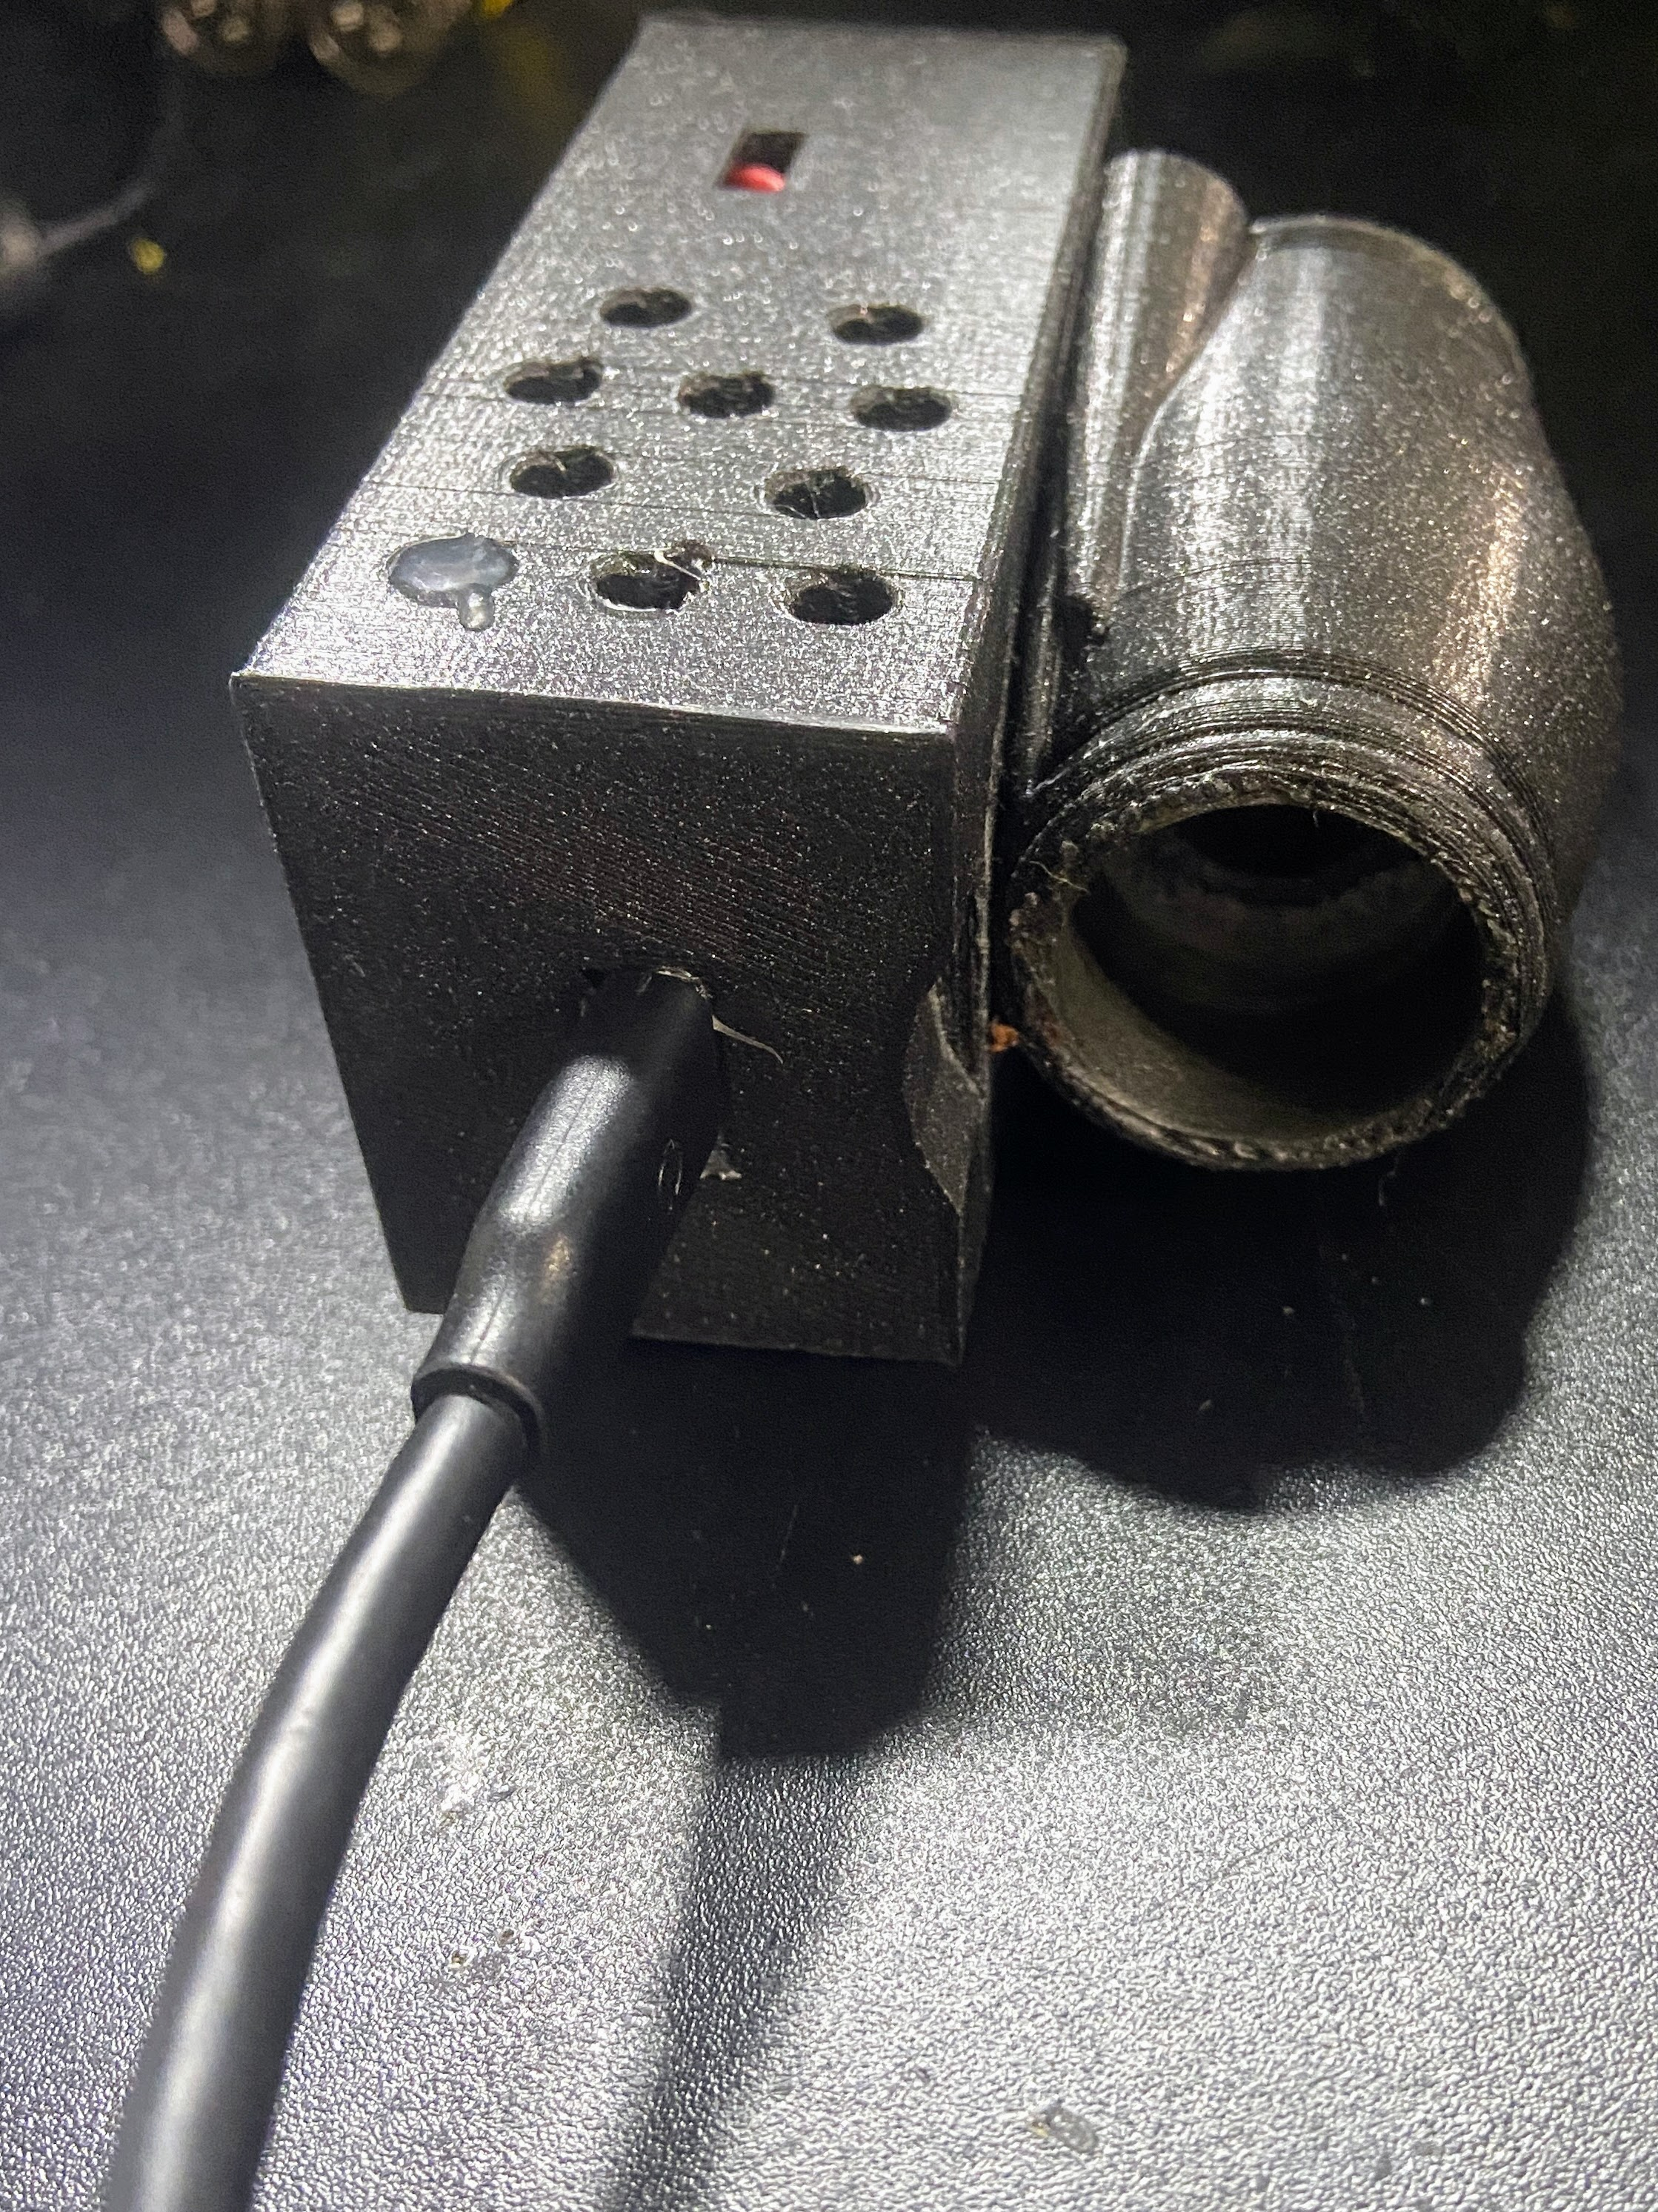
\includegraphics[scale=0.08]{diagrams/IMG_2208 (1).JPG}
    \caption{Charging the Cyberinet}
    \label{fig:chargeUnit}
\end{figure}

\subsection{I2C Sensors}
While all of the sensors in the Cyberinet utilize the same OEM compatibility features, not all sensors are the same. The Gyroscope/Accelerometer, Differential Airflow Pressure, and Thermometer are all I2C sensors, which have their own unique protocol. Due to wire routing constraints, all of the expansion units are intentionally \emph{not} I2C components, while the sensors embedded within the main unit are.

I2C sensors are able to communicate with a host device through their titular data protocol. This is a serial data connection\footnote{a conceptually similar protocol to USB devices connected to a computer.} where both the host device and the attached sensor are able to directly communicate with each other with a syncing clock. While individual sensors may vary, the I2C sensors in the Cyberinet only need the clock and data connections (along with power and ground) in order to function. This helps to reduce the number of traces needed on the PCB, making it easier to design and manufacture.

Looking back to the pins on the ESP-32 micro-controller used in the Cyberinet, only one of each of those pins are present. So how can the two sensors communicate with the controller without the data becoming corrupted? The answer is perhaps the greatest strength of I2C communications. Devices using I2C communicate on specific addresses. This means that multiple sensors can all connect to the same clock and data pins, and each will work as long as they are utilizing unique addresses. Because the address is represented as a 7-bit value, the maximum number of potential I2C devices that can be connected to a single host is 127. In practice this number is usually lower because a single sensor can potentially utilize multiple addresses, but is still more than enough connections for the Cyberinet to utilize.


\subsubsection{Gyroscope \& Accelerometer}

The main motion-detecting sensor utilized in the Cyberinet is the MPU-6050. This is a commonplace sensor containing a six degree-of-freedom gyroscope and accelerometer. The board also contains a thermometer, but this one is not utilized. The MPU6050 communicates on I2C address 0x68., but this can be changed to allow for an additional 6050 to connect to the same host.

\begin{center}
    \begin{figure}
        \centering
        \includegraphics[scale=0.3]{diagrams/GY-521_MPU-6050_Module_3_Axis_Gyroscope_+_Accelerometer_0487.jpg}
        \caption{MPU-6050 Gyroscope and Accelerometer}
        \label{fig:6050}
    \end{figure}
\end{center}

Within the integrated circuit (IC) shown in the center of figure \ref{fig:6050} are the micro-electromechanical systems (MEMS) components for the gyroscope and accelerate. These incredibly small components are able to interact with each other and bridge specific connections in order to determine which direction the device is moving, and how quickly that movement occurs\cite{6050HowTo}. The Cyberinet utilizes only the top four pins (VCC, GND, SCL, SDA) to receive data. The additional pins can be used in other scenarios, but are ignored here. Using the serial clock connection (SCL), the ESP-32 and the MPU-6050 are able to communicate along the data pin (SDA).  


\subsubsection{Differential Airflow Pressure \& Thermometer}

Originally released in 2017, the SDP-31 is the newest individual hardware component utilized with the Cyberinet. This unit detects differential airflow pressure between two points as well as temperature. Due to the SDP-3X line’s small form factor, the Sparkfun Qwiic connector breakout board was selected for simple, OEM compliant installation. Two small tubes are attached to the ports and used to measure the air pressure difference between the inside of the Cyberinet barrel and the outside of the instrument. This is the same tube as shown in figure \ref{fig:msgLED}.

\begin{center}
    \begin{figure}
        \centering
        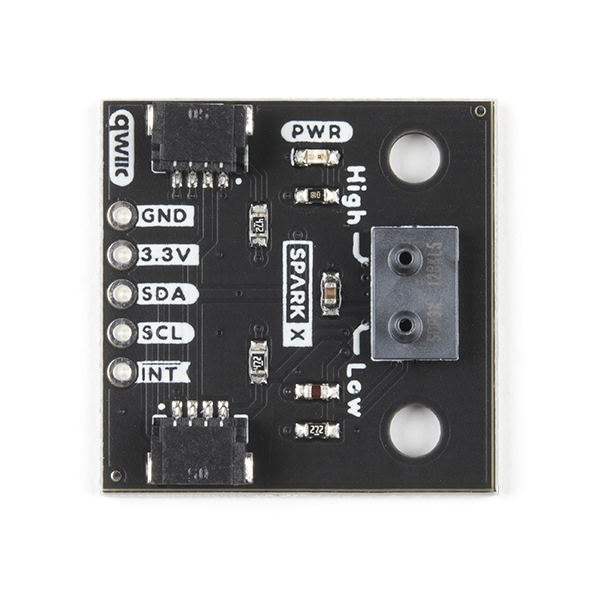
\includegraphics[scale=1.5, angle=90]{diagrams/oem/spd31.jpg}
        \caption{Sparkfun SDP-31 Differential Airflow Pressure Qwiic Connect Breakout Board} %replace with my picture
        \label{fig:sdp-31}
    \end{figure}
\end{center}

A differential pressure sensor functions by placing a diaphragm in between two pressure points. In the SDP-31, this MEMS is located in between the two hose attachments. As the pressure between the two areas changes, the diaphragm position will move, and this movement is captured electronically to represent the difference in pressure between the two points\cite{airflow}. Because of it’s higher accuracy, the SDP-31’s temperature sensor is utilized over the MPU-6050. Temperature is measured in degrees Celsius. This sensor utilizes address 0x21 be default, but by cutting or bridging pads on the bottom of the breakout board this address can be changed to one of three possible options depending on the specific use case.

The Cyberinet utilizes all pins accept the interrupt (INT). This pin can be used to request data at a specific time, but since the Cyberinet is constantly sensing and transmitting data, it is not needed.

\subsection{Optional Expansion Sensors}
In addition to the built-in I2C sensors, the Cyberinet utilizes a variety of optional expansions that can be implemented as needed to customize the array of sensors. The main expansion unit contains two momentary push buttons and LEDs. As previously mentioned, these sensors are \emph{not} I2C sensors, and utilize specific pin combinations without the serial protocol. At the time of writing, one expansion unit has been completed, with plans for additional expansions already underway.

\subsubsection{Button Expansion}

The Button Expansion is much simpler when compared to the main unit. The unit is composed of only two mechanical buttons with built in LED's, two resistors for those LED's, a USB-C port for communication with the Main Unit, a PCB to route all of the connections and the 3D printed housing. The button expansion is designed to be attached to the performer's thumb rest to allow for easy access with the right thumb. However it is also shaped in a way to allow for it to be held in the hand or placed elsewhere.

\begin{center}
    \begin{figure}
        \centering
        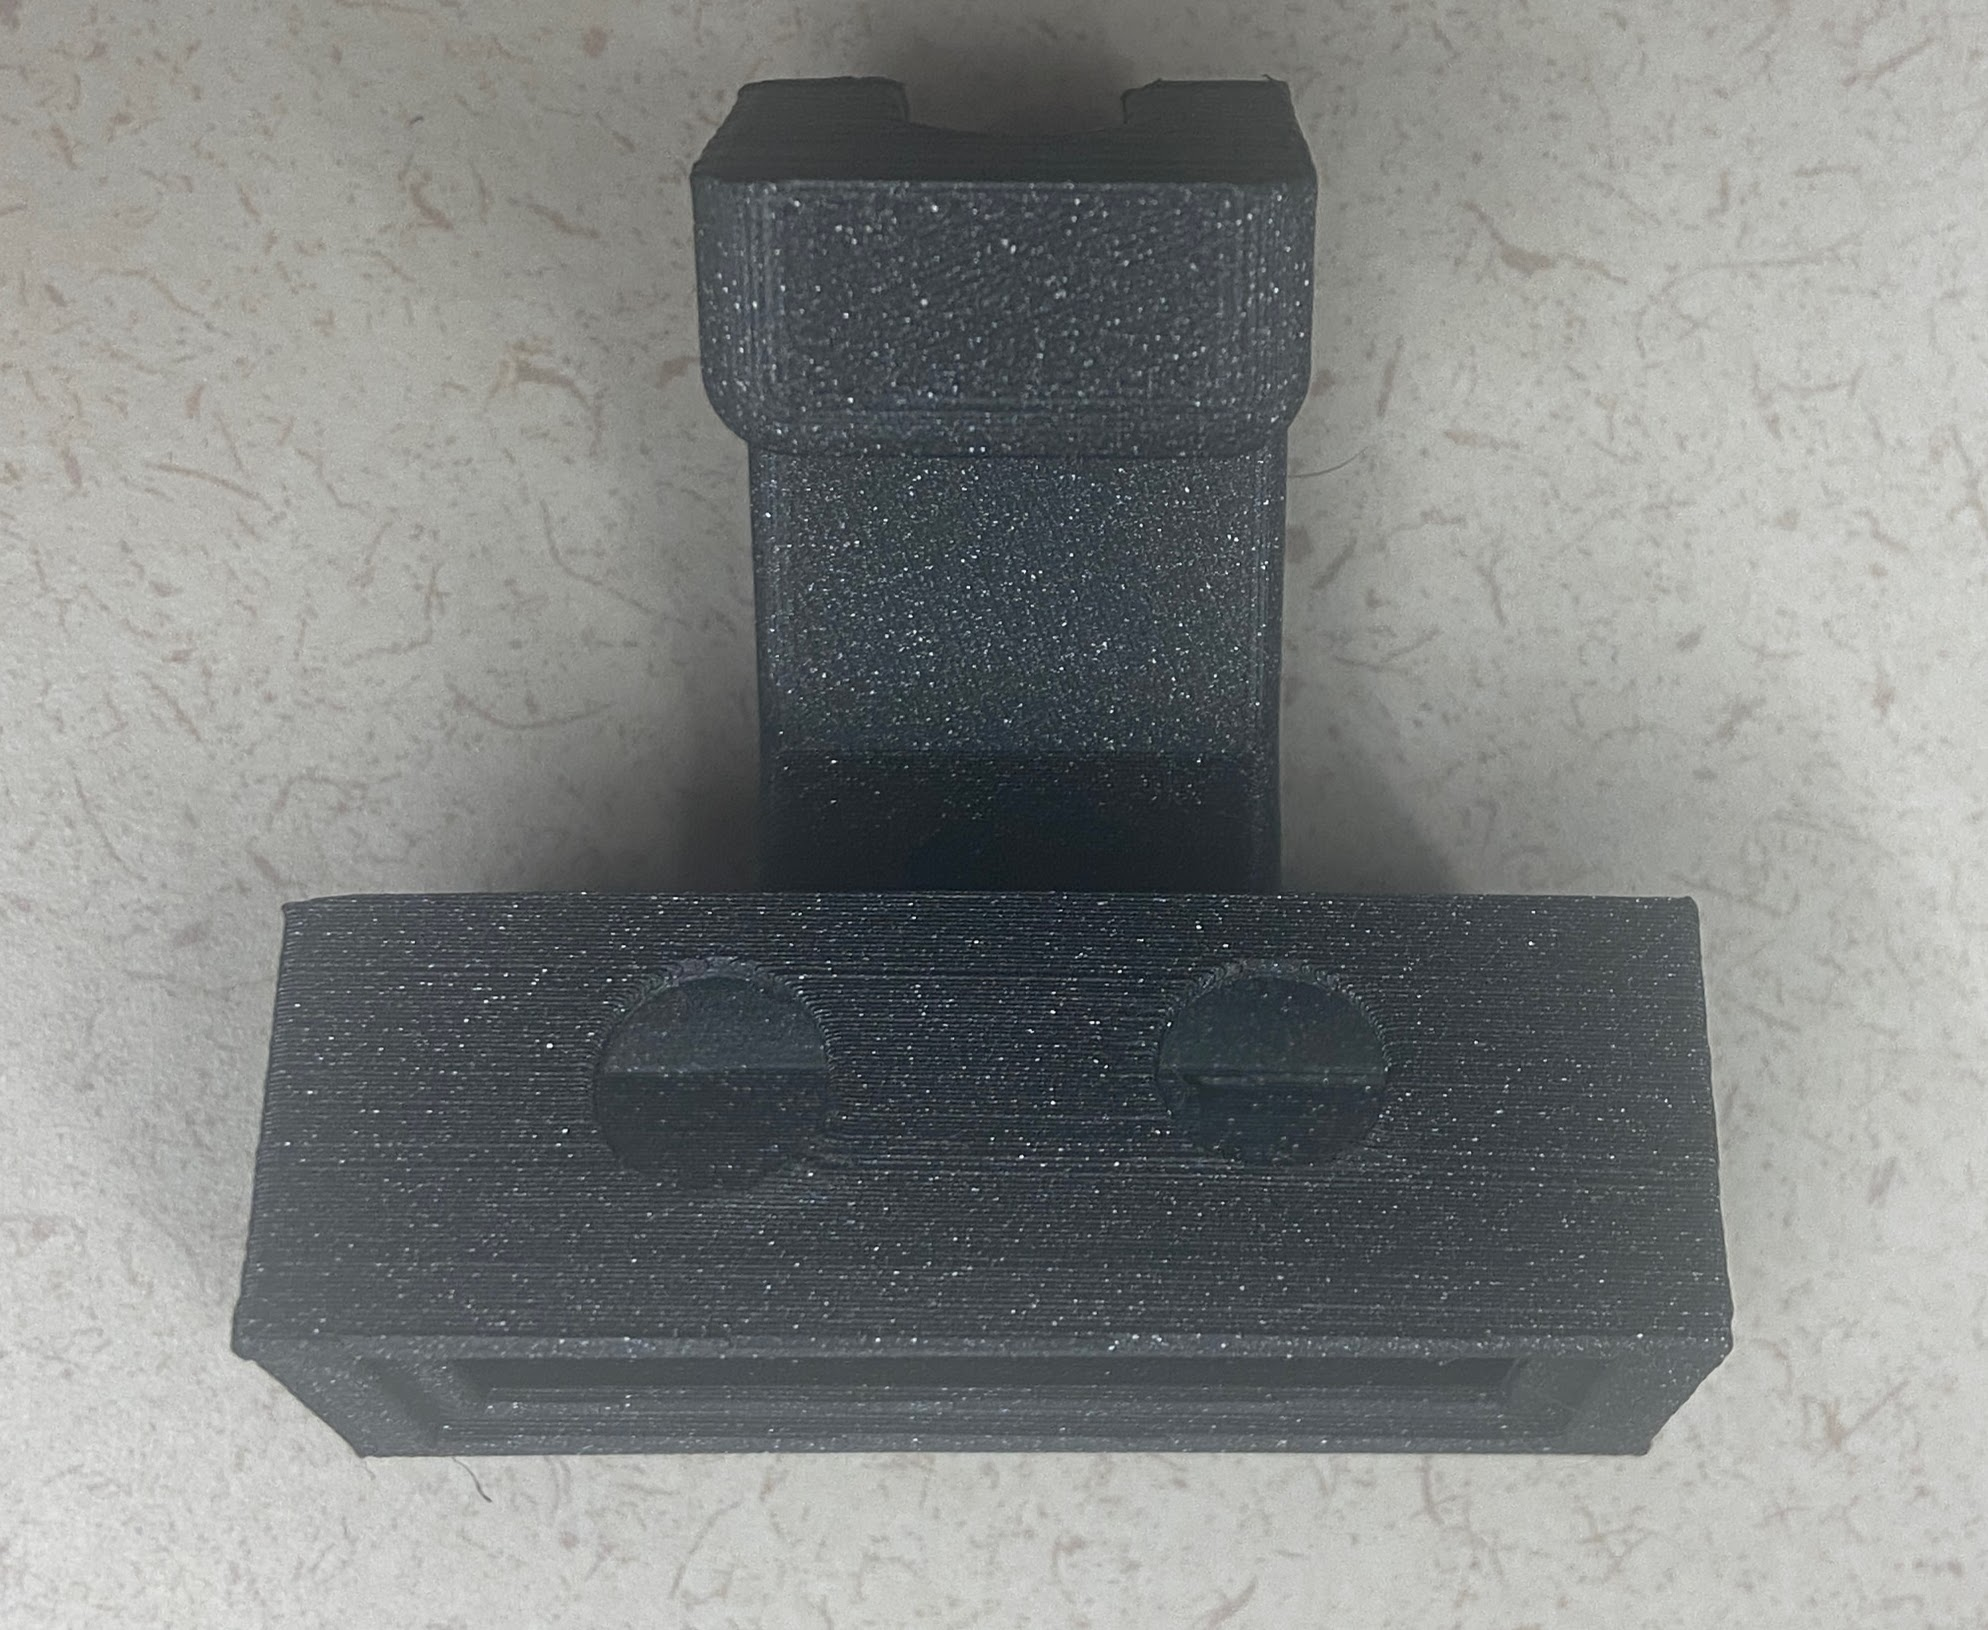
\includegraphics[scale=0.1]{diagrams/builtUnits/buttonhousingEmpty.JPG}
        \caption{Empty 3D-printed thumb rest with housing for buttons below.}
        \label{fig:buttonThumbrest}
    \end{figure}
\end{center}

To assemble the unit, all components are soldered to the PCB. In a similar manner to the main unit, SMD components are attached first, followed by cables, and finally the larger components, the buttons, last. This process of assembling from smaller-to-larger components is present in all parts of the Cyberinet.  The completed PCB is then secured within the 3D-printed housing to complete the unit. The PCB for the Button Expansion is shown in figure \ref{fig:buttonPCB}, and the version of the PCB containing all of the components soldered to it is part of figure \ref{fig:CyberinetNoCase}.


\begin{center}
    \begin{figure}
        \centering
        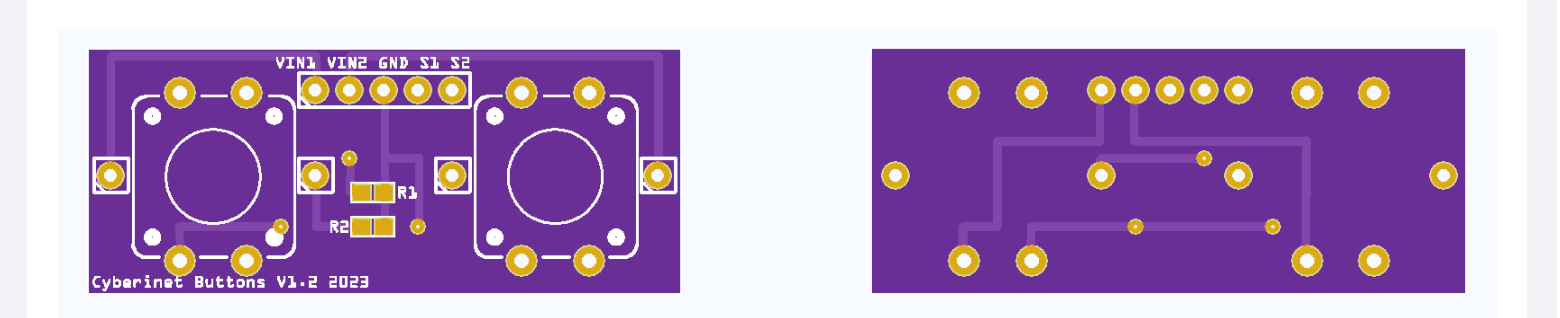
\includegraphics[scale=0.5]{diagrams/PCBs/buttons1.2.png}
        \caption{Button Expansion PCB}
        \label{fig:buttonPCB}
    \end{figure}
\end{center}


Expansion Units are optional and not needed for the Cyberinet main unit to be functional and are intended to only be connected when needed for a particular performance. All the expansions connect utilizing a standard USB-C connector. However, these units do not utilize the USB protocol, so both the main unit and expansions cannot be connected to a computer via these ports. While a set of USB-C cables that are functional is included with the full Cyberinet set of hardware, The main reason for utilizing this connector is for the end-user to be able to supply their own cables of various lengths depending on their needs. 


\begin{center}
    \begin{figure}
        \centering
        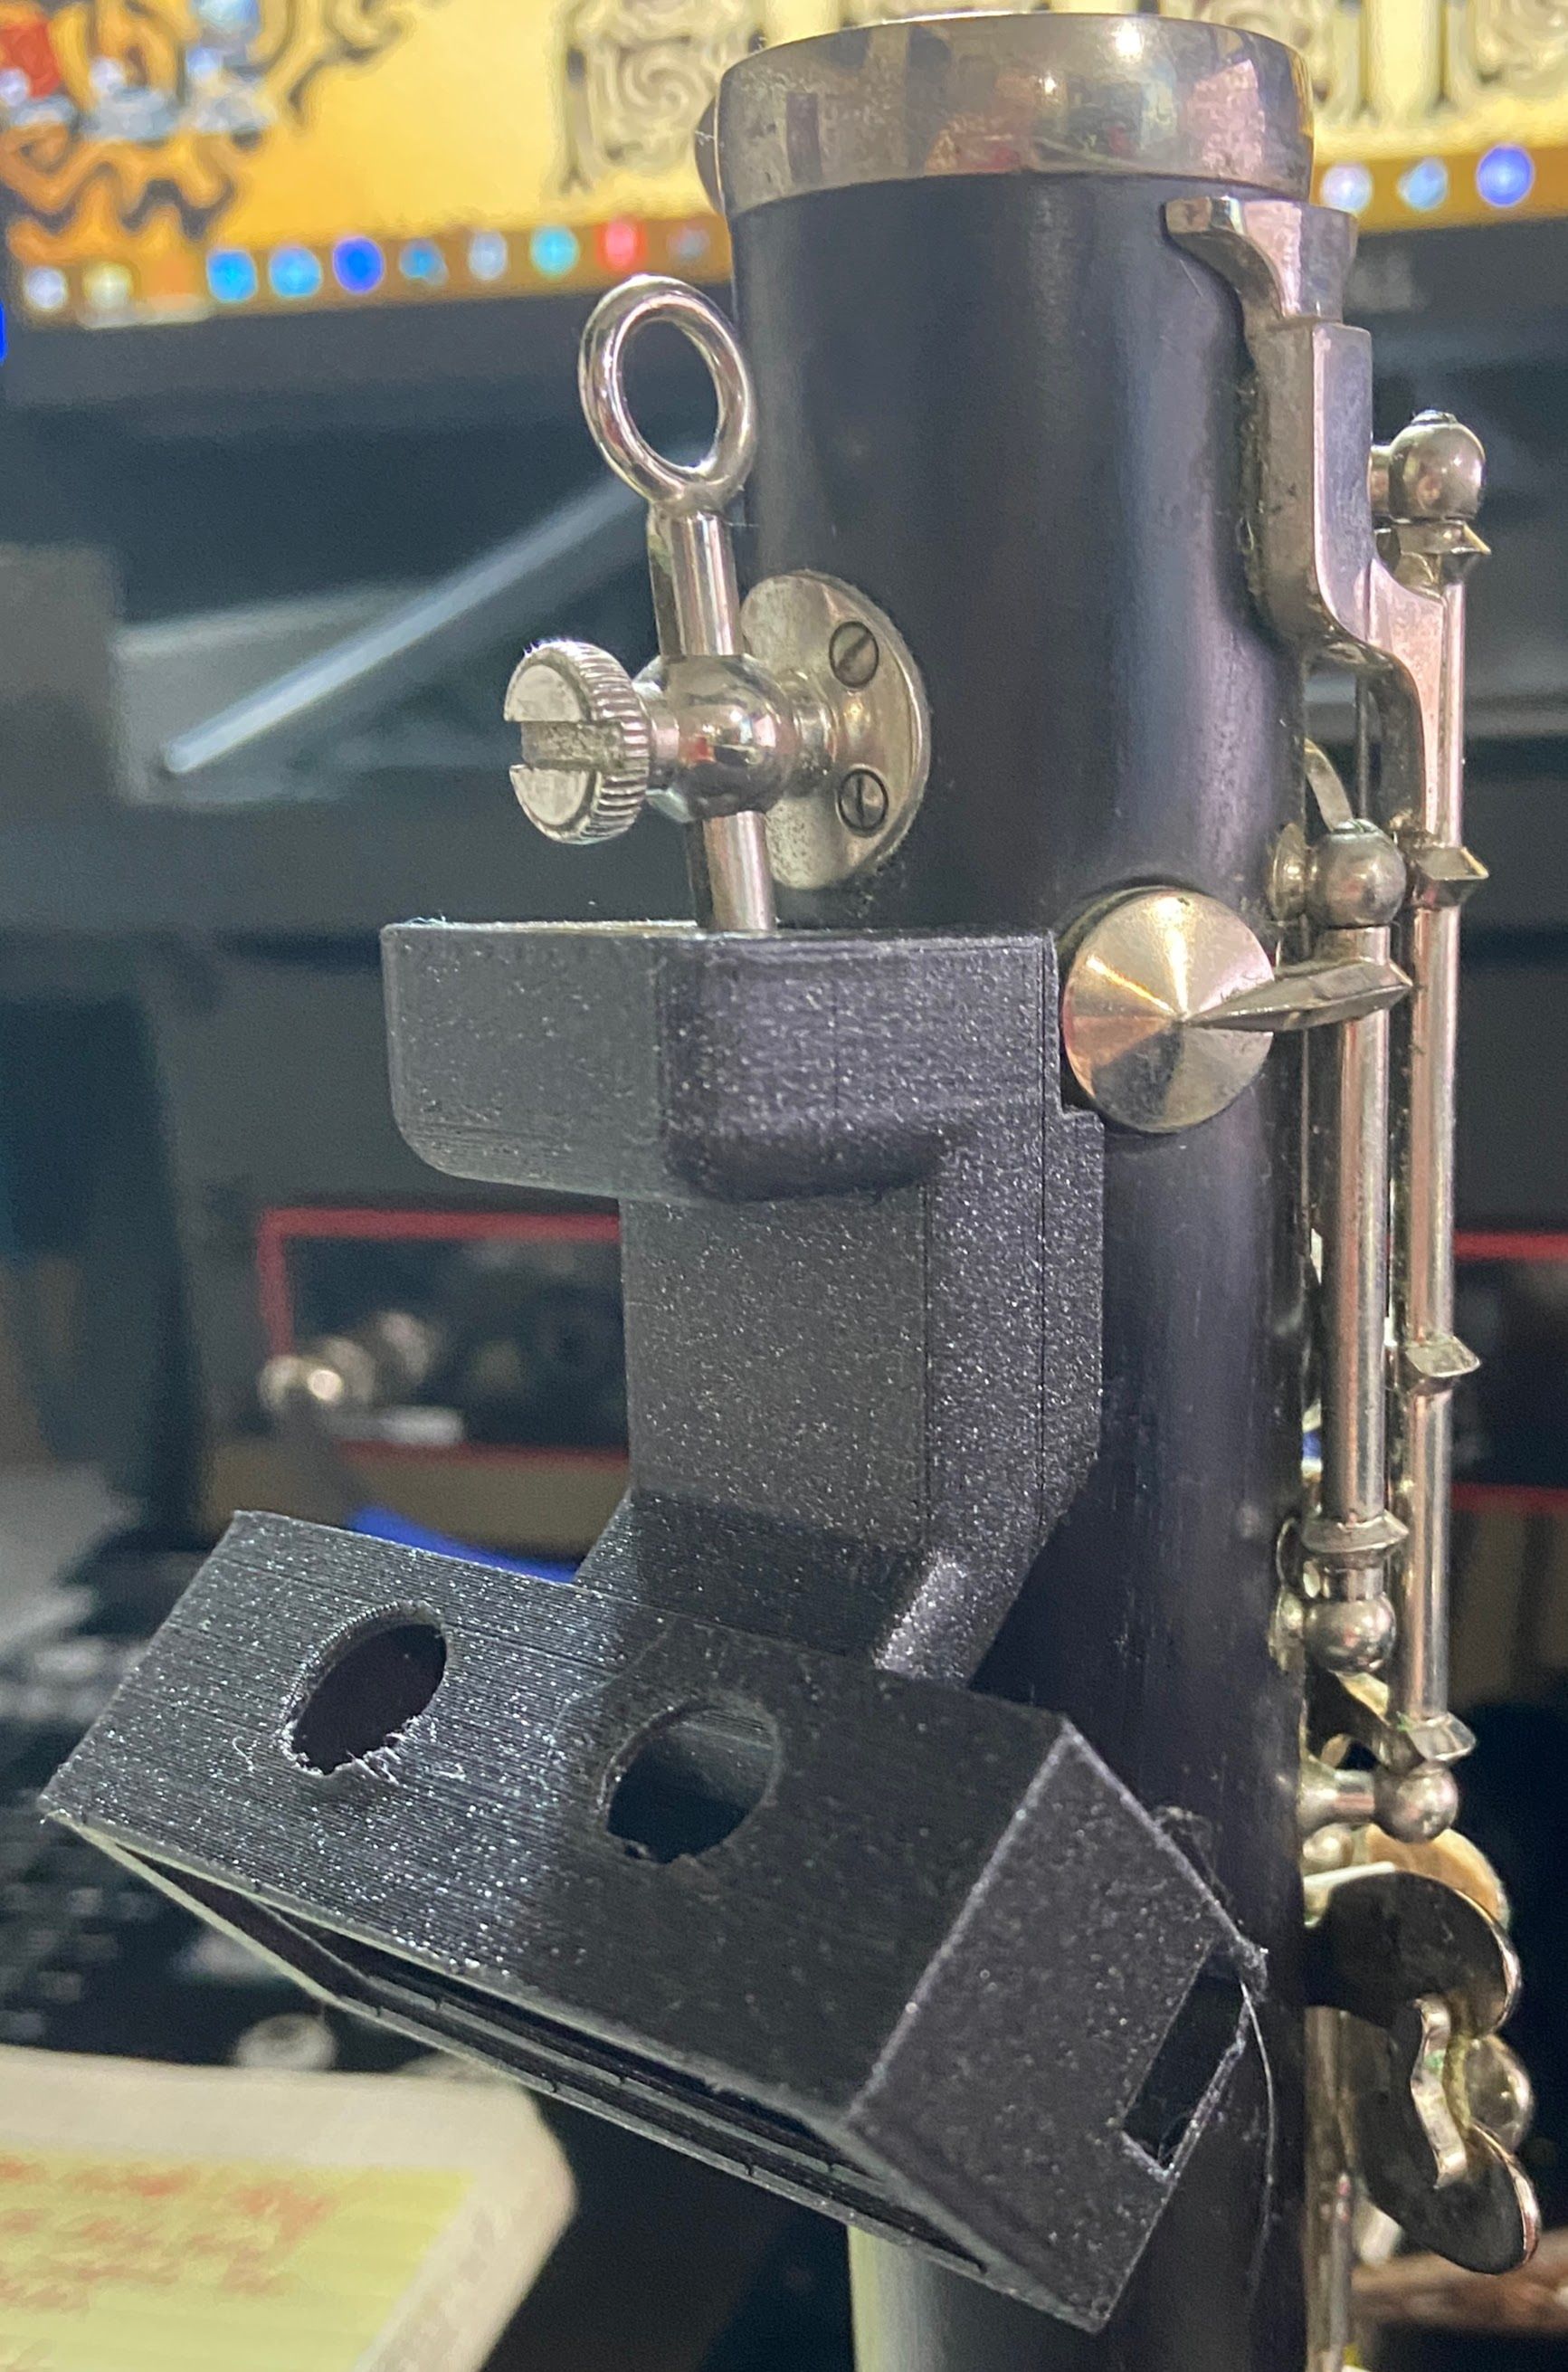
\includegraphics[scale=0.08]{diagrams/builtUnits/thumbOnInst.JPG}
        \caption{Empty Button Expansion placed on a Clarinet thumb rest}
        \label{fig:thumbOnCase}
    \end{figure}
\end{center}

The button expansion, while optional, is incredibly useful for a performer on stage. They can access the buttons using their right thumb when performing. The closeness between the buttons and thumb rest is shown in figures \ref{fig:buttonThumbrest} and \ref{fig:thumbOnCase}\footnote{The case has been revised since the initial picture was taken. The small rectangular hole for the connection cable has been moved to the left side to avoid potential collisions with the performer's hand.}. The performer can also place the buttons elsewhere if they like using a longer connector cable. The housing for the buttons is also designed to be a little larger than is necessary to allow for a more ergonomic feel should the performer choose to hold the expansion. Each button also contains a single, colored LED built into it to provide feedback to the performer. By default, the lights are only illuminated when the button is pressed. The Cyberinet simply detects whether a button has been pressed and transmits that data as a Boolean value to the computer. Using Max, the user can have the buttons achieve functions from near limitless hypothetical list of options. For this project, the buttons were used to trigger microphone recording and buffer playback, however objects that take the button input, move between various presets, trigger DSP, and turn pages of a score have also been developed and included in the software bundle for the Cyberinet.

Because of the usefulness of this unit, it is given its own connection port on the Cyberinet so that the user does not have to choose between this and another sensor. Referring back to table \ref{tab:mainPins}, pins 12 and 14 of the ESP-32 detect when the buttons are pressed, and pins 26 and 27 turn on each button's built-in LED.

\begin{figure} %crop image if I have time
    \centering 
    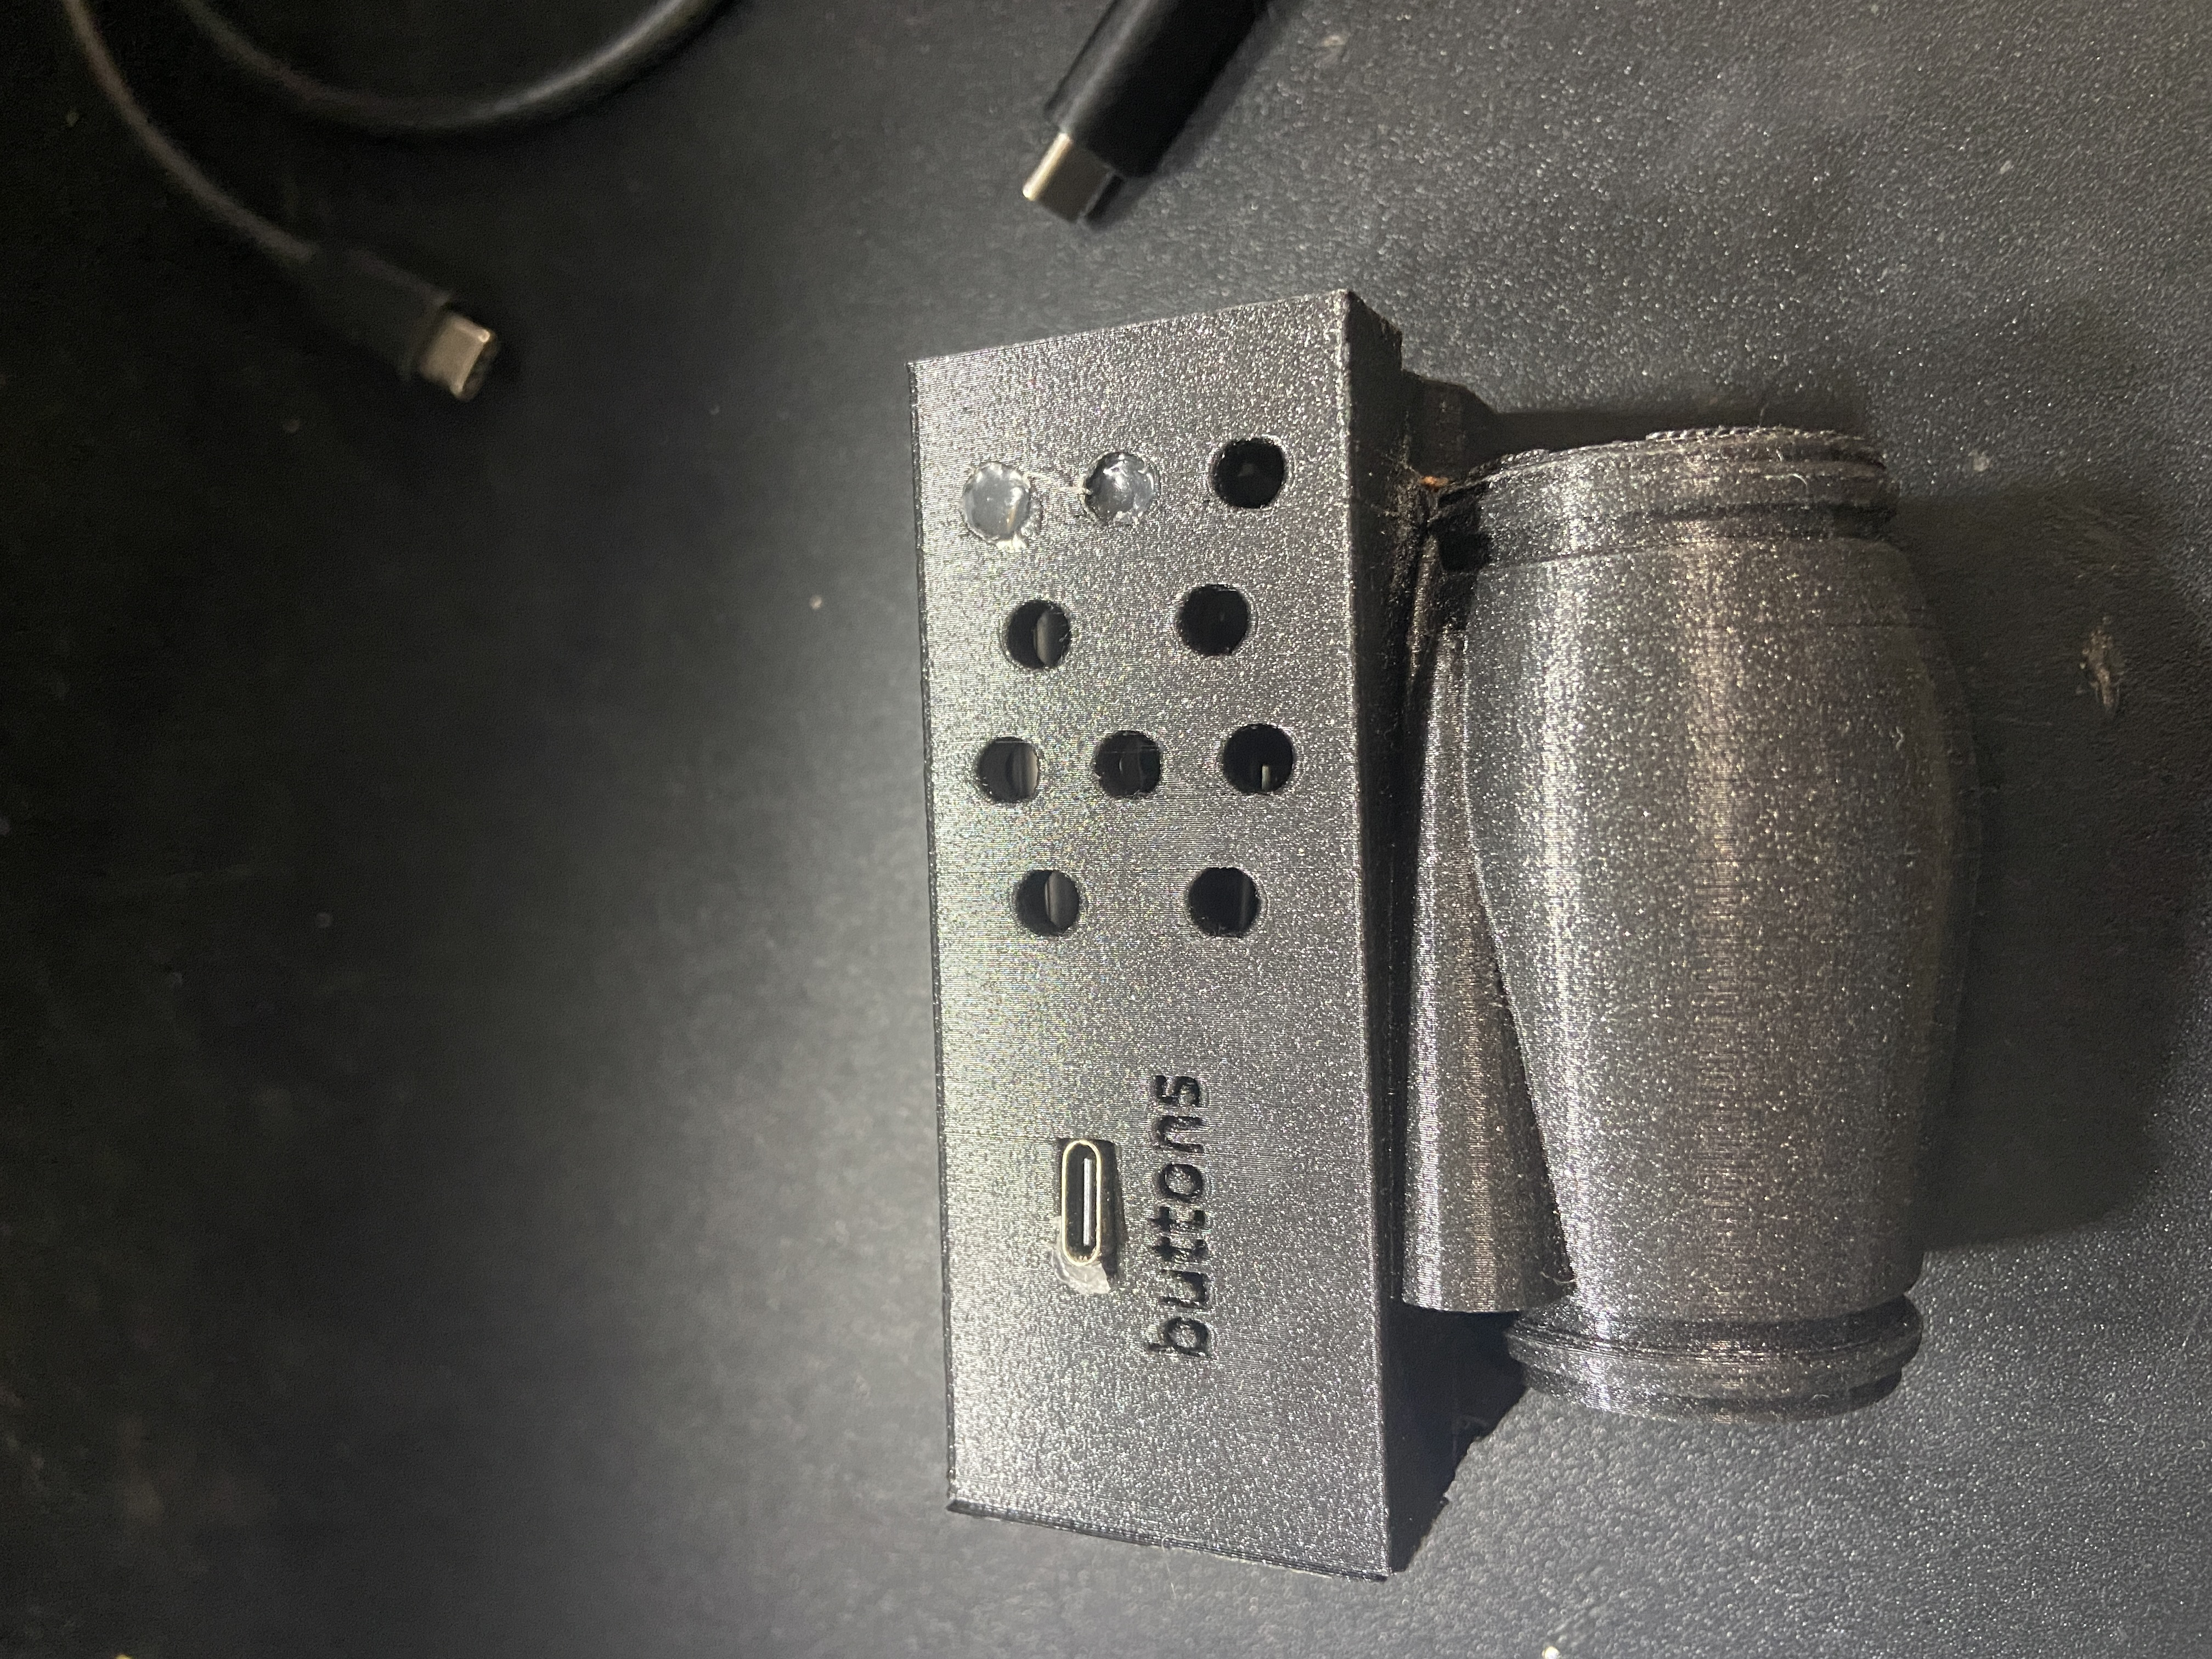
\includegraphics[scale=0.05, angle=270]{diagrams/builtUnits/buttonPort.JPG}
    \caption{Location of the Button Expansion port on the Cyberinet.}
    \label{fig:buttonPort}
\end{figure}

The port for the buttons is located on the upper portion of the Cyberinet main unit in order to reduce the amount of wire needed to reach the PCB, as well as to visually distinguish it from the charging port. Because a differing number of pins is used between this and the other expansion port, located in the same location on the opposite side of the unit, is given the label "buttons". The main unit can be rotated 360 degrees in order to adjust the positioning of the button expansion cable to wherever the performer desires.

\subsubsection{Other Expansions}
At the time of writing, only the button expansion has been developed and tested completely. However, in-progress plans for a continuing range of expansions exist.

The joystick expansion is relatively simple. It is designed to receive data from the single button and two potentiometers of a standard joystick. The PCB diagram shown in figure \ref{fig:jsPCB} shows the simplicity of this setup. Power and ground are received and fed to both the joystick as well as the power indicator LED. The values from the horizontal position, vertical position, and button are all returned to the ESP-32 on pins 33, 32, and 35 respectively. When transmitting to the computer, the data receives the labels exp1, exp2, exp3, and exp4. All expansion units receive the same labels with a different number because they are interchangeable. This removes the need for a the unit to have to identify the expansion and apply the appropriate label. The number specifies the pin that the data is receiving, and the connectors of the physical units are wired to consistently begin with exp1 and utilize up to the four available pins.

\begin{figure}
    \centering
    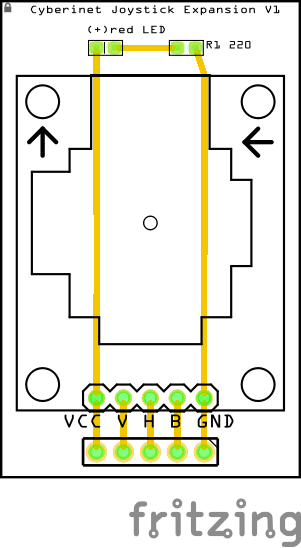
\includegraphics{diagrams/PCBs/thumbPCBv1.png}
    \caption{Joystick Expansion PCB diagram}
    \label{fig:jsPCB}
\end{figure}

As shown in the middle of the board, there is space for a daughter board to be attached. This is the Sparkfun BOB-09110 breakout board, which serves as the interface between the COM-16273 Joystick Deluxe the board shown in figure \ref{fig:jsPCB}. When soldered, the voltages are passed through to the 5 pins at the bottom, which are wired with a ribbon cable to the USB-C port similar to the button expansion. The deluxe joystick was selected because of its higher-quality construction compared to other joysticks on the market, and the ability to easily swap tops to allow for a variety of interface options and feelings for the performer. Outside of construction quality however, the joystick is a standard device, which helps to keep the cost of the unit manageable.

\begin{figure}
    \centering
    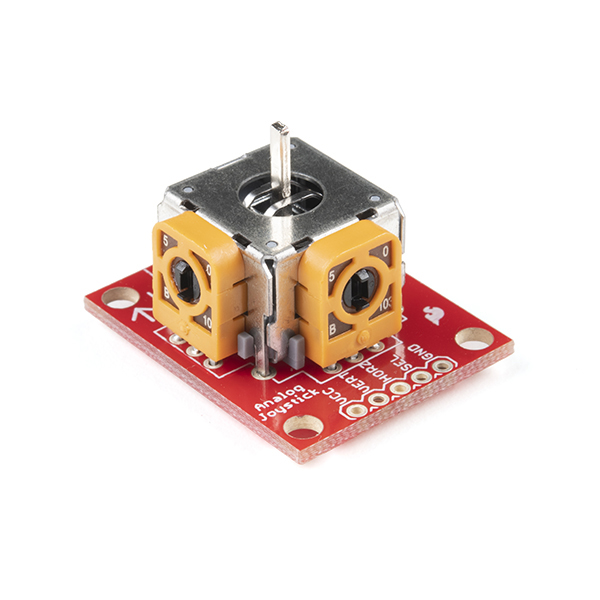
\includegraphics[scale=1.2]{diagrams/oem/16273-Thumb_Joystick_-_Deluxe-03.jpg}
    \caption{Joystick on BOB-09110 Breakout Board, from sparkfun.com}
    \label{fig:js2}
\end{figure}

The element of the unit remaining to be designed at this moment is the 3D printed housing. This is intended to attach to the Clarinet in place of the button expansion, allowing for three different elements of control on the thumb rest. However, utilizing the button expansion thumb rest with the joystick has proved less ergonomic than desired, and will be fine tuned.

The Volume Detection unit contains a uxcell Microphone Sound Sensor Voice Detection Module. Like the Button expansion, this unit is housed in a 3D printed case and connects to the Main unit with a USB-C cable. The PCB diagram shown in figure \ref{fig:micExPCB} is perhaps the least complex of all of the boards created so far. It essentially acts as an extension from the breakout module to the USB-C connector. Like the joystick and main PCBs, there is a place to include the power indication LED. The module will sit on the majority of empty space on the board, and should be pointed towards the desired pickup area. If loose, a little glue can be used to help hold the module down to the PCB. 

\begin{figure}
    \centering
    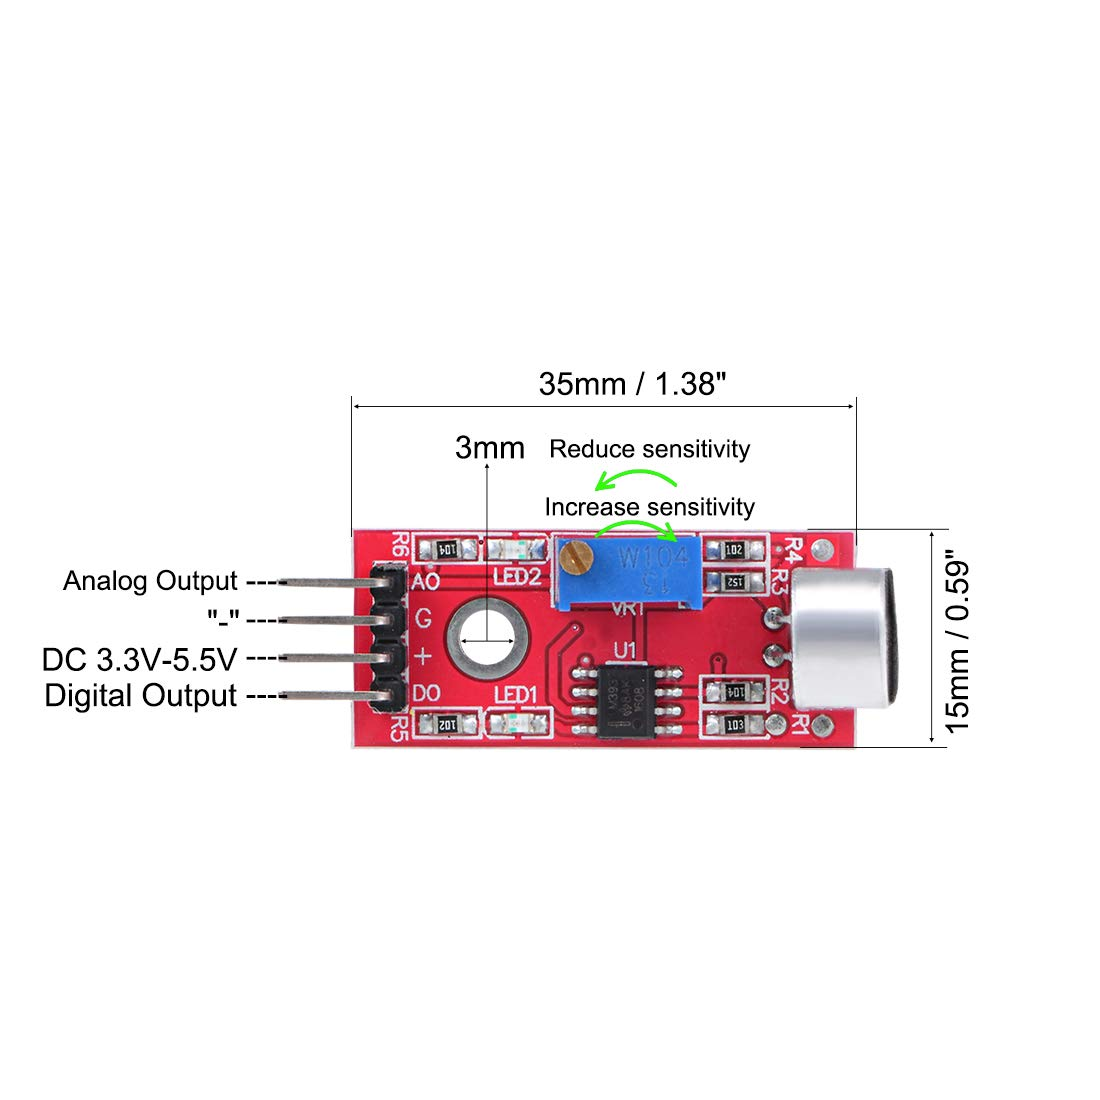
\includegraphics[scale=0.3]{diagrams/mic.jpg}
    \caption{uxcell Microphone Sound Sensor Voice Detection Module. Photo from amazon.com listing}
    \label{fig:micExpansion}
\end{figure}

\begin{figure}
    \centering
    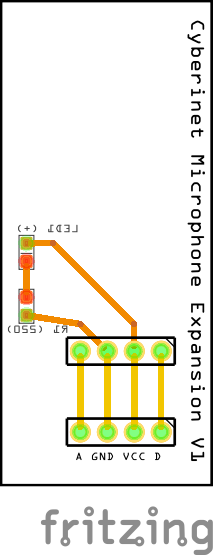
\includegraphics[angle=90]{diagrams/PCBs/micBasic_pcb.png}
    \caption{Microphone Expansion base PCB}
    \label{fig:micExPCB}
\end{figure}

This unit is designed to respond to the volume of the local area, and is designed to be placed in a variety of different areas. By placing the sensor at different distances from the performer or speakers, the sensor can to the volume levels. The sensitivity can be adjusted with an on-board potentiometer and screwdriver. The user is only limited by the length of USB-C cable they can utilize. The Cyberinet detects when the volume at the sensor exceeds the given threshold from the on-board potentiometer, and transmits the data as a Boolean value to the computer in a similar manner to the Button Expansion. Future revisions will explore the uxcell Microphone Sound Sensor Voice Detection Module's analog outputs, but for now version 1 will only be utilizing the digital output due to its simpler and more reliable use cases. Ground and power connect to the middle two pins, and the data is returned on the pin marked D in figure \ref{fig:micExPCB}. This data is transmitted using the label exp1. 

Like the joystick, the 3D case is the final element keeping this unit from being further developed at the time of writing. The case is intended to entirely cover the microphone with the exception of holes for sound pickup, threshold adjustment, and viewing the LED. The case is also intended to have a clip that can be used to attack it to various objects such as a music stand or the bell of the Cyberinet. Unlike the joystick expansion however, prototype testing has not begun.

\section{Physical Design}
In order to minimize the total number of parts required to assemble the Cyberinet, the electronics are housed in a newly designed plastic unit. This Main Unit is intended to replace the barrel and mouthpiece of the original instrument when in use. In addition to the main unit, all expansions have a 3D printed body in order to control the expansion's ergonomics, protect the electronics, and aesthetically match the main unit.

\begin{center}
    \begin{figure}
        \centering
        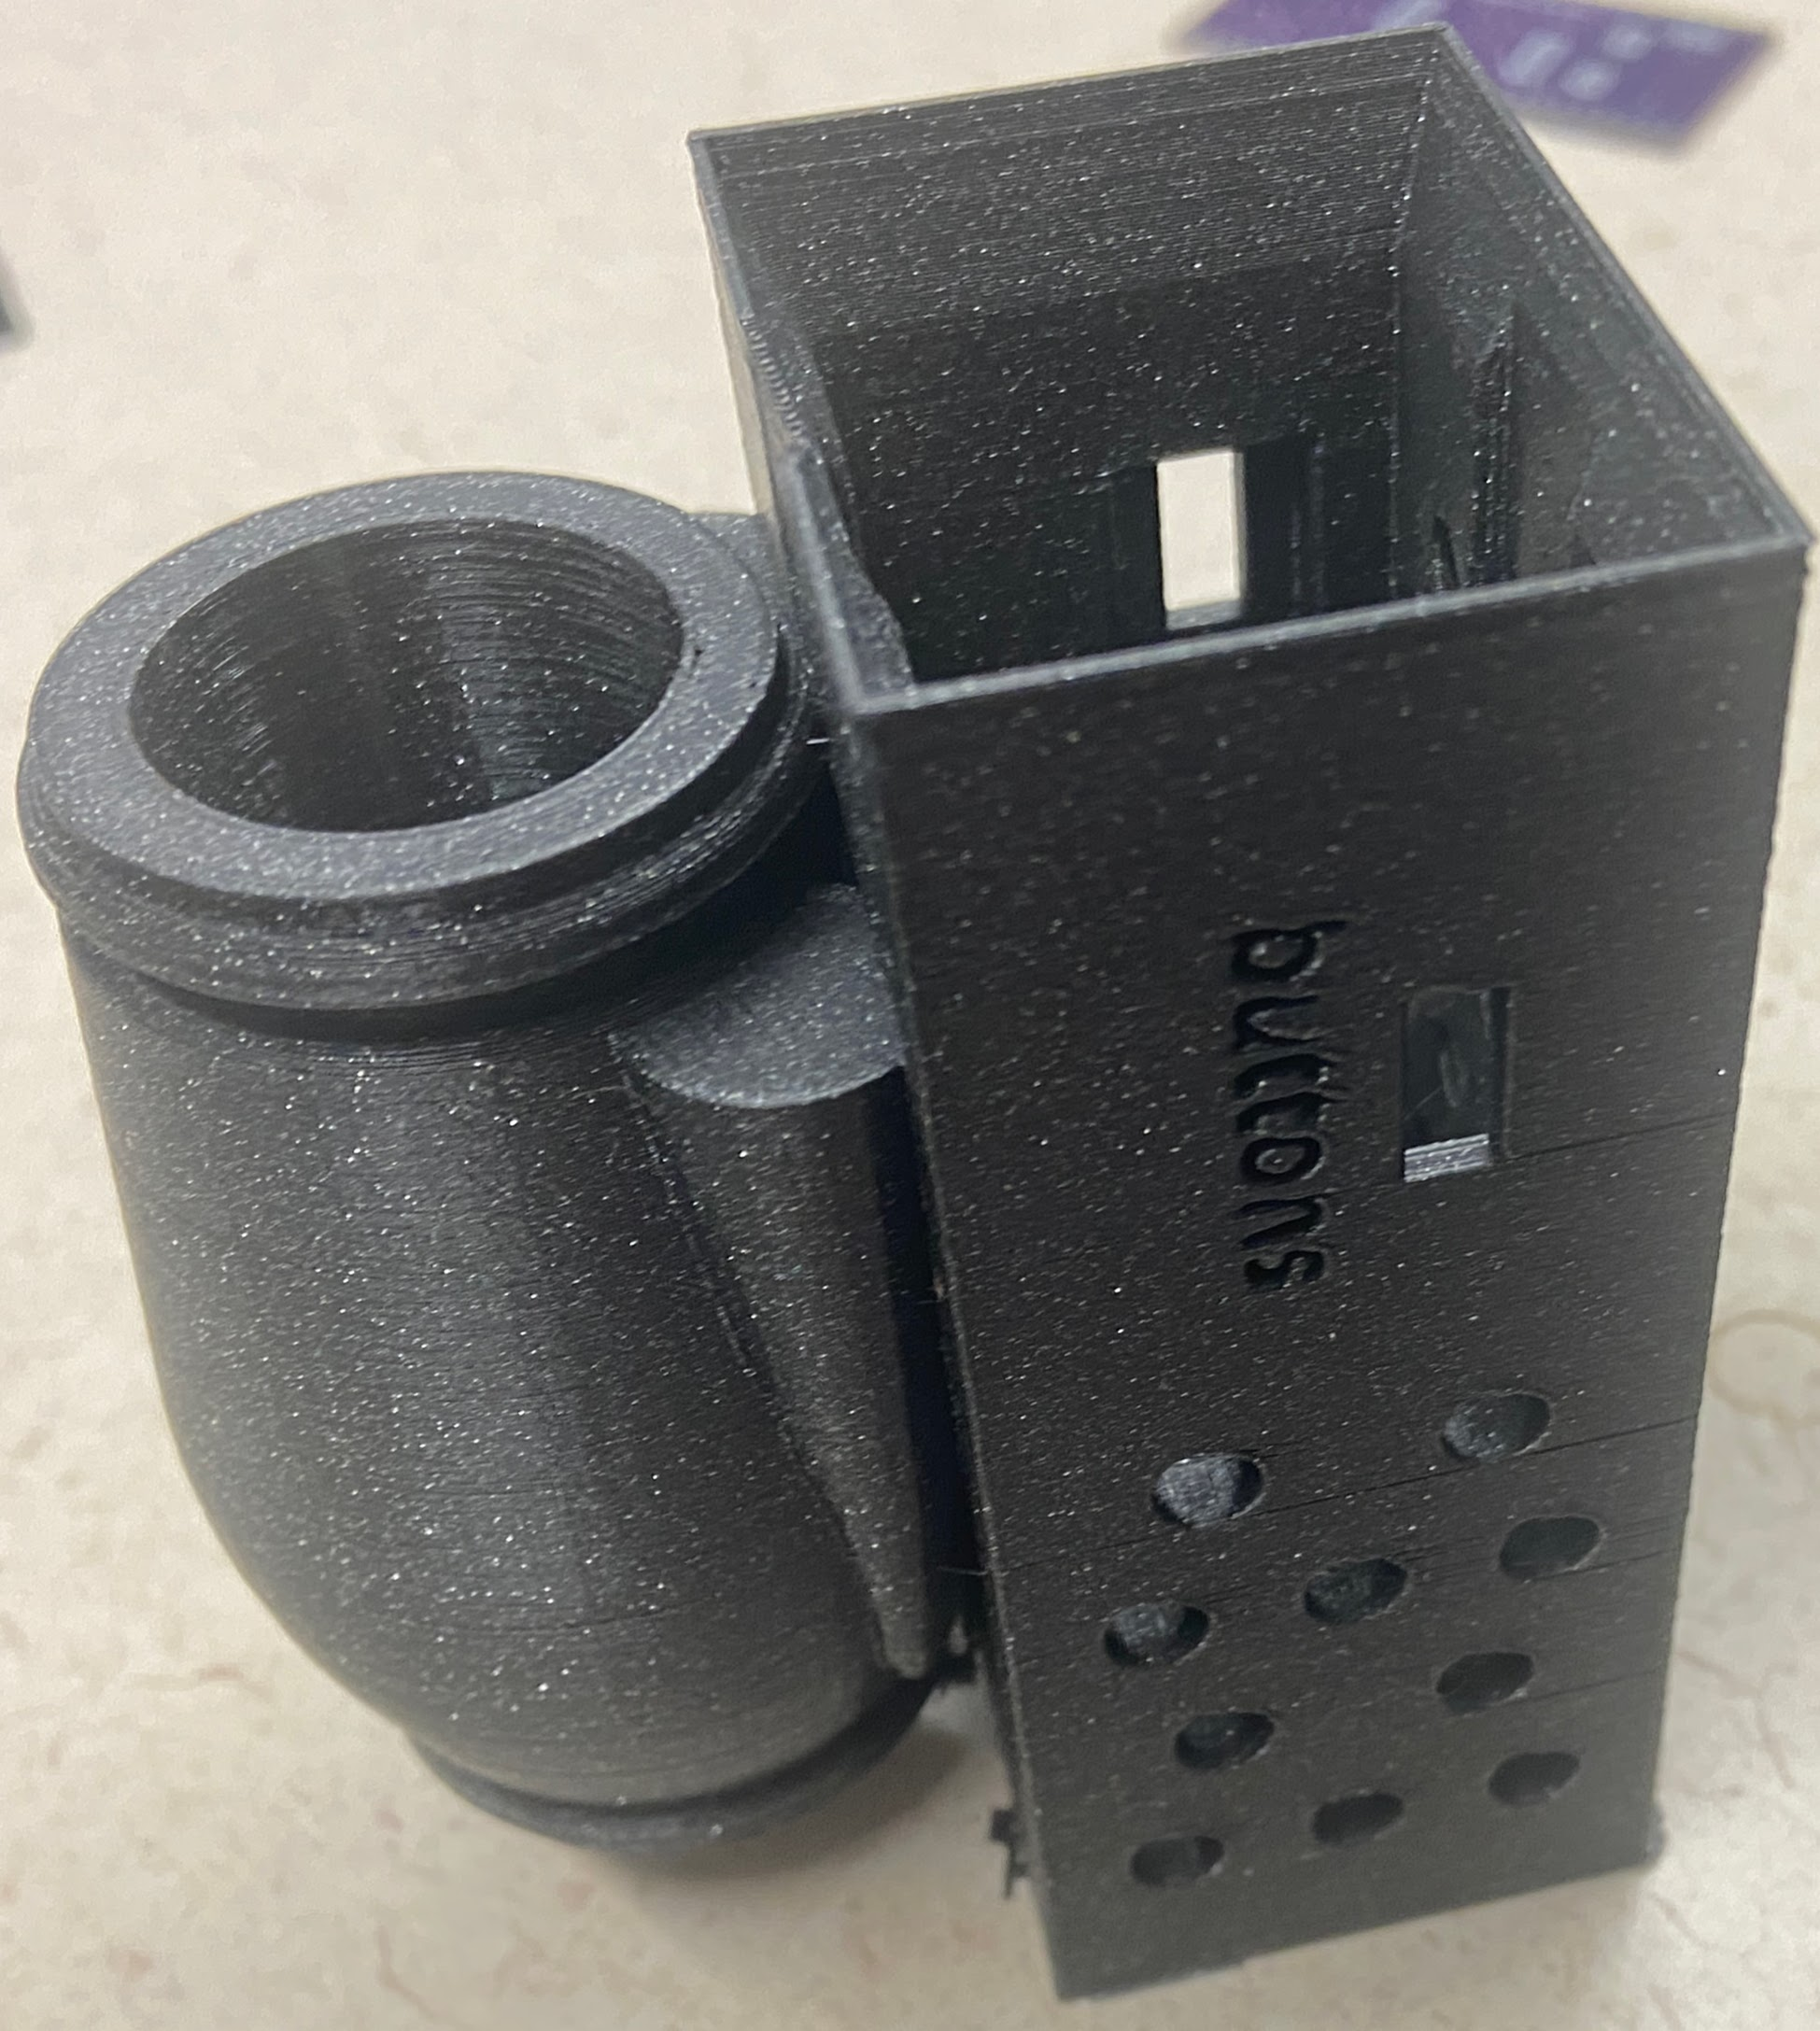
\includegraphics[scale=0.1]{diagrams/builtUnits/emptyCase.JPG}
        \caption{Empty 3D Printed Cyberinet Housing}
        \label{fig:cybernetCase}
    \end{figure}
\end{center}

All cases are printed using either PLA or PetG material during prototyping. These materials were chosen for their relative low cost, ease of production, and density. For the final version, PLA was utilized because the sound quality of the material most closely resembled that of the original Clarinet. All parts were printed on an Original Prusa i3 MK3S+, with a 30-40\% infill setting. The final version was printed to be black or dark grey, however future revisions could see an option for custom colors when printing.

The main unit case consists of two main parts. The lid is the smallerst part, and contains both clips to hold the lid in place, as well as holes to insert the power switch and airflow tube into. The larger 3D printed component is shown in figure \ref{fig:cybernetCase}, and began as a model of a Clarinet barrel. From there the various components were measured and the box was attached to the side of the barrel. The various holes and supports were added last in order to give the Cyberinet more structural integrity, especially when being removed from the Clarinet.


\subsection{Cyberinet Assembly}

The main unit of the Cyberinet is designed to replace the barrel of the base Clarinet. As shown in figure \ref{fig:cybernetCase}, the electronic components are housed in the box on the side of the instrument. Placing the electronics here allows for the unit to be easily adjusted for tuning or be removed as needed. The box was made as small as possible, but it still contains all of the electronic components, excluding those in any external add-on components. 

The electronics were housed in the upper portion of the Clarinet for two main reasons. The more minimal of the reasons is that the differential airflow pressure is much greater in the Clarinet before the air can escape through the key holes. By locating the sensor here a wider range of values are possible than if it was located lower on the Clarinet's tube. However, this could be remedied with additional tubing if the location of a unit needed to be otherwise located. The second reason is that by placing the unit above the player's hands, it helps to keep the Cyberinet away from the performer's hands, allowing them to finger various notes without worrying about bumping the device.

To assemble a Cyberinet main unit, first the case must be 3D printed. Because of the process of 3D printing with the necessary density of material needed to preserve sound quality, the printing process takes approximately 12 hours to complete. Because of this, it is recommended to begin printing the case first, then work on the remainder while the case is being completed by the printer. All components housed within the case are connected utilizing a custom printed circuit board. This is done to help connect all of the various pins for data collection and power distribution in as small of a space as possible. 

\begin{center}
    \begin{figure}
        \centering
        \includegraphics[scale=0.6]{diagrams/PCBs/CyberinetPCB.png}
        \caption{Cyberinet Version 1.3  Main Unit PCB Diagram}
        \label{fig:mainUnitPCB}
    \end{figure}
\end{center}

Assembling the Cyberinet must be done by working with the smallest components and working up to the larger ones. This is because several components are placed over other ones and it becomes exponentially harder to assemble a Cyberinet should one have to begin working around the placement of a sensor or remove a chip to adjust or repeat a step\footnote{It is recommended to pause and check the connections after soldering each component for this reason as well.}. This approach is also taken when assembling the various expansion units as well.

First, the Surface-Mounted components are soldered onto the main board. These include the 2 on-board LEDs and their accompanying resistors. Following this, ribbon cables and the USB-C and JST connectors are then soldered into place on the PCB. The ribbon cables are located on the five and six pin sections in the middle of figure \ref{fig:mainUnitPCB}. The connections for the button expansion and the other expansions are labelled due to the differing number of pins and their arrangement for the units. The JST connector is attached to the traces labeled GND and Batt. These connections attach the the USB-c connectors and the 1200 mAh battery respectively.

The third step is to solder the power distribution (TP-4056), gyroscope (MPU-6050) and airflow pressure (SDP-31) chips into place. The white silkscreen rectangles show which side of the PCB each component belongs on, and the text indicates which orientation is needed for each component to help ensure a correct alignment\footnote{This is also true for the connections that have already been mentioned.}. The airflow pressure sensor (SPD-31) is lifted away from the PCB with the use of a pin header. This is done to avoid any accidental shorts between the contacts on the two boards. While not required, this can be done to the gyroscope (MPU-6050) as well for the same reason. The final soldering step is to connect the ESP-32. Because of its size, this chip is kept opposite from the sensors and is also lifted using pin headers to avoid any accidental short circuits. Because there are no connections underneath the TP-4056, this chip can be placed directly onto the PCB for a thinner connection.

\begin{center}
    \begin{figure}
        \centering
        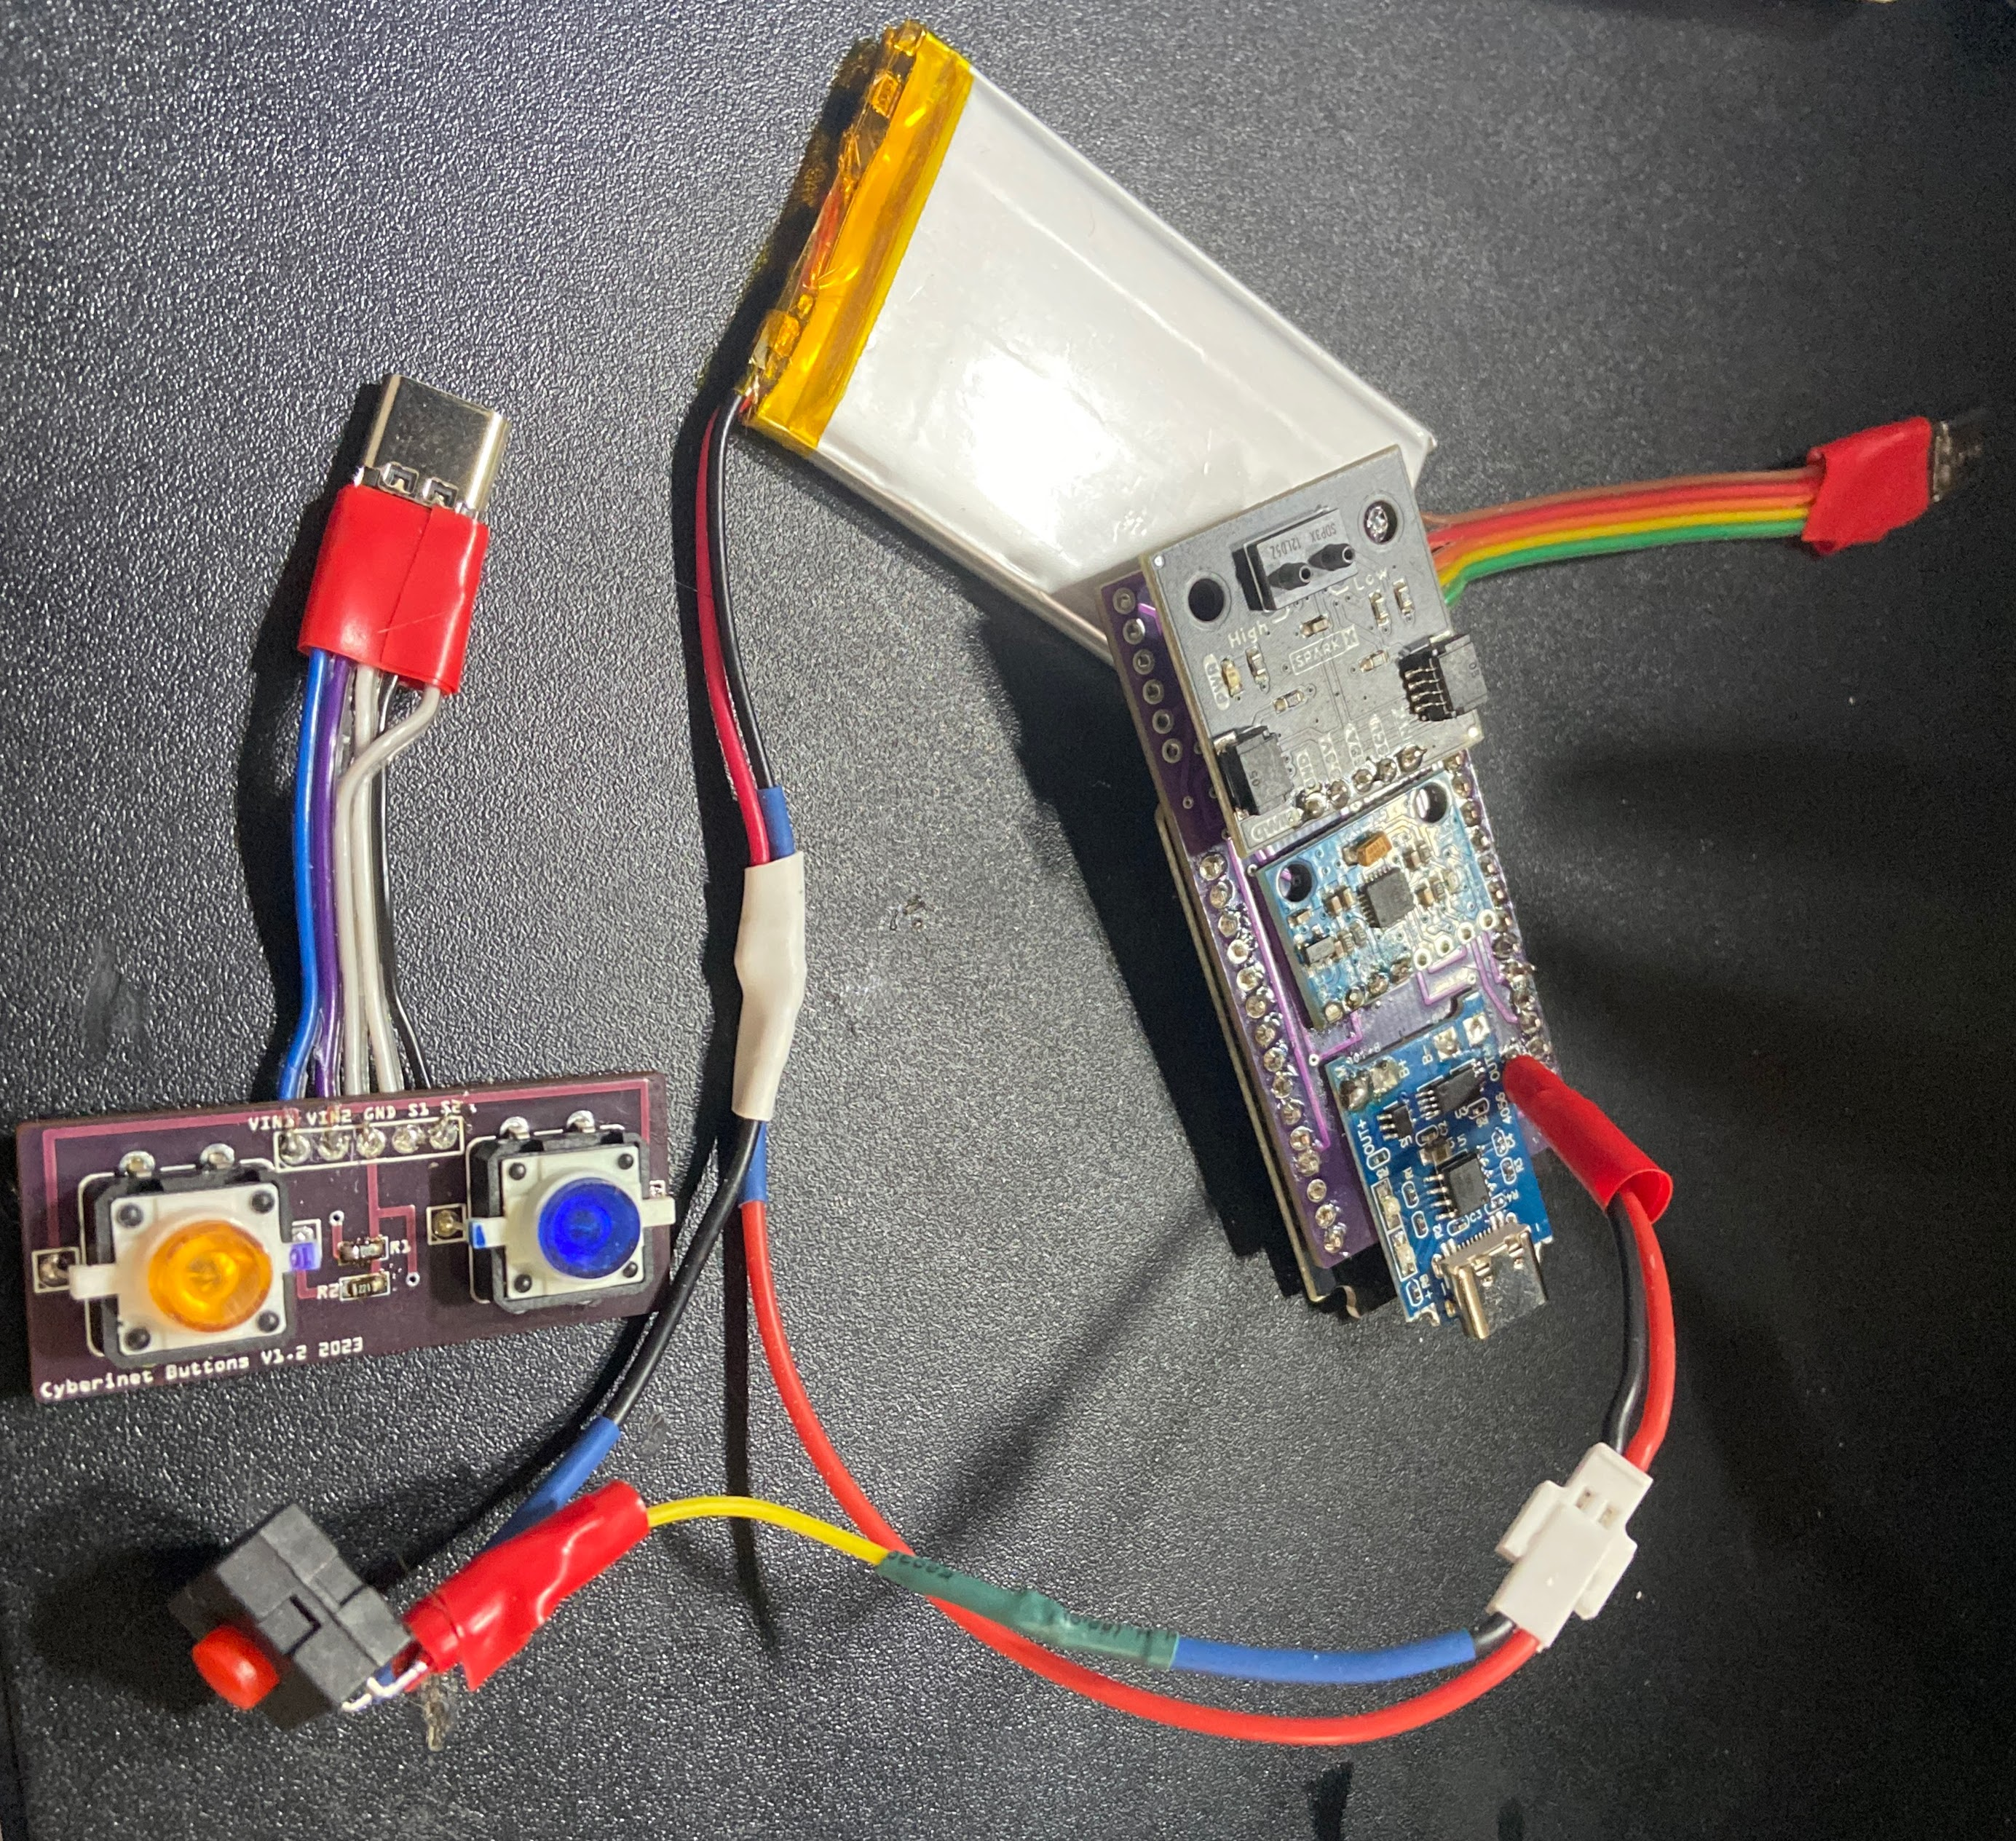
\includegraphics[scale=0.1, angle=90]{diagrams/builtUnits/noCase.JPG}
        \caption{Completed Cyberinet and Button Expansion without 3D printed housings.}
        \label{fig:CyberinetNoCase}
    \end{figure}
\end{center}

When complete, the whole unit is slid into the 3D-printed case. Ports and tubes are aligned to the appropriate places and glued down to avoid unwanted movement. Not taking into account the space needed for the battery, tubing, and wires, the final Main PCB is approximately 5mm deep, creating a compact unit that can be easily placed in a variety of locations. When the battery is included, the depth is approximately 9mm.

\begin{center}
    \begin{figure}
        \centering
        \includegraphics[scale=0.05]{diagrams/PCBs/CyberinetThin.JPG}
        \caption{Cyberinet Sensors Side View (No Casing or cables)}
        \label{fig:Cyberinetside}
    \end{figure}
\end{center}

Once the internal electronics have been inserted, secured, and sealed into the 3D printed case, it is ready to be fully tested. Because the Cyberinet unit cannot be easily opened, and will require glue to reseal, it is recommended that all base functionality be tested prior to closing the housing. While close, no two Clarinets are completely identical, so the internal sides of the 3D printed case may need to be sanded to properly fit onto the Clarinet with cork grease applied. Overall, placing the Main Unit's bulkiest components as close to the performer's mouth as possible results in the least amount of extra effort required to perform with the instrument. It is impossible to completely remove the added weight of the system additional, but this placement minimizes its impact on the performer.


\chapter{Programming \& Using the Cyberinet}
This chapter discusses the code located within the Cyberinet itself, as well as the accompanying library of Max tools and how they can be utilized in a performance. The Arduino code and the Max objects work together in order to achieve the five main steps in the functionality loop of the Cyberinet. These steps will be utilized in order to organize the discussion of the various code elements of the Cyberinet.

\begin{itemize}
    \item Step 1: Collect Data
    \item Step 2: Transmit Data
    \item Step 3: Receive Date
    \item Step 4: Route Data
    \item Step 5: Utilize Routed Data
\end{itemize}

The functionality is not a full loop from steps one to five. By this I mean that once the data has been transmitted, the hardware will repeat the sensing and transmitting process while the computer will route and apply the data in a separately timed loop. The communication is not two-way between the computer and hardware unit, but the computer-side loop is unable to begin without the completion of the hardware loop. Combined with data smoothing within Max, the end result is a constant stream of data between the two with minimal latency.

\section{Arduino Code}
A positive feature of the ESP-32 is that it is able to be programmed utilizing a variety of languages and environments. For the Cyberinet, the micro-controller was programmed using the Arduino coding language and Arduino IDE version 1.8\footnote{Arduino IDE Versions 2.0 and 2.1 were both released during the Cyberinet's development, but were not utilized to avoid any potential compatibility issues during development. Future software versions will be created in more up-to-date IDEs.} The full .ino file can be found in this document's appendices.

\subsection{Collecting Data}
In order to collect the data from the sensors, each sensor has been given a function within the Arduino code. These functions serve the main focus of collecting and transmitting data. However because of the differing OEM sensors, each one utilizes a slightly different method of data collection and has a different range of values that can be expected. These functions are called in every loop of the program. Figure \ref{fig:getButtonsGetAir} shows the two most straightforward of these functions in their entirety.

\begin{center}
    \begin{figure}
        \centering
        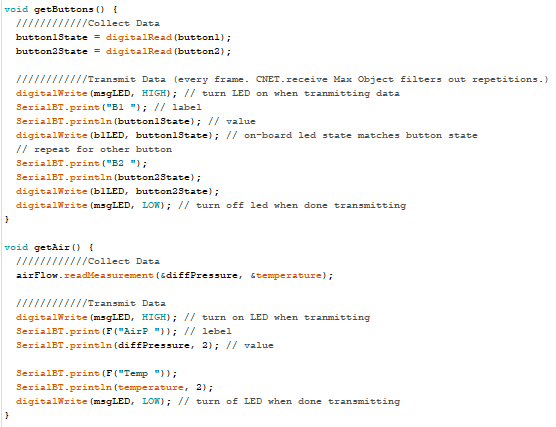
\includegraphics[scale=1.5]{diagrams/maxPatches/getbuttonsgetair.png}
        \caption{Cyberinet getButtons() \& getAir() functions.}
        \label{fig:getButtonsGetAir}
    \end{figure}
\end{center}

getButtons() is the simplest of these functions. This function looks at pins 12 and 14 on the ESP-32, which are connected to the Button Expansion's USB-C connector. By utilizing the ESP-32's built-in pull-up resistors, the Button Expansion returns a 1 when the button is not being pressed and a 0 when the button has been detected as being clicked, thus completing the circuit. The expansion units function is effectively identical to getButtons(). The only differences are which pins are being referred to within each loop.

getAir() works in a similar function to getButtons(), but with a slightly different code because of the SDP-31's I2C connection and coding library. Because of this, the ESP-32 contacts the SDP-31 on its I2c address and requests the specific data at 2 registers. These data are labelled as 'diffPressure' and 'temperature' respectively. 

The function 'get5060()' is shown in figure \ref{fig:get6050}, and contains a few more steps than the previous functions. This function begins by communicating with the MPU-6050; essentially waking it up after having communicated with the SDP-31 on the same pins. Next, the six data points for the gyroscope and accelerometer are requested like 'diffPressure' and 'temperature'. It is at this point that the function begins to differ from the others.

\begin{center}
    \begin{figure}
        \centering
        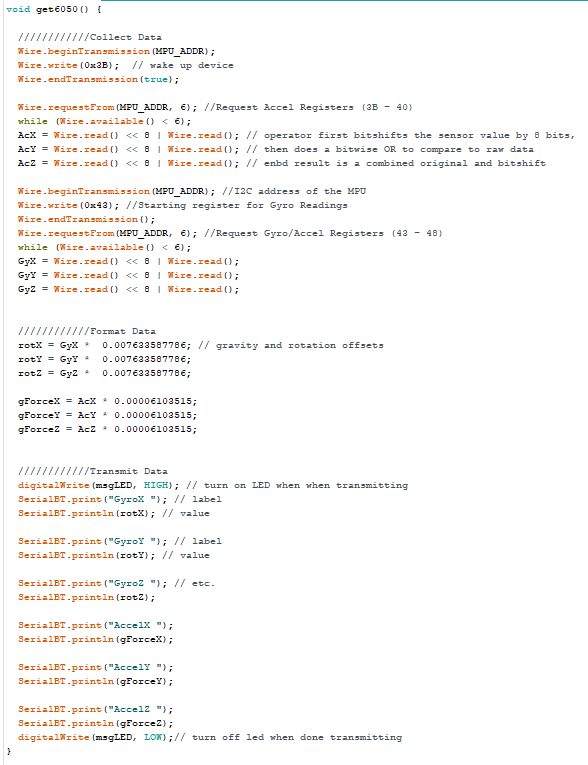
\includegraphics[scale=1.5]{diagrams/maxPatches/get6050.png}
        \caption{Cyberinet get6050() function.}
        \label{fig:get6050}
    \end{figure}
\end{center}

All six of the requested data points are then shifted over by 8 bits and then added to a second reading of the remaining data. This is done in order to fully read all 16 bits of data from the MPU-6050 on devices unable to access and process all 16 bits of data at once. Prior to transmitting the data, the values from the MPU-6050 are then scaled. This is done to compensate for both the gravitational pull and rotation of the earth, allowing for more accurate results. This step is done here rather than in Max to eliminate the potential of a user not scaling the data within Max.


\subsection{Transmitting Data}
The final portion of the data collection functions is the transmission of the data. This is done using the bluetoothSerial library, which allows for the ESP-32 to utilize serial communications over a Bluetooth connection. The .ino code's setup function is responsible for initializing these connections. The port is titled "CyberinetV13", indicating the version number with no spaces or punctuation, and utilizes a baud rate of 115200\footnote{In short, the baud rate is the number of changes to the state changes within a digital signal.Larger values allow for more data transmission, if the device is capable of handling the increased data rate}. This library contains the Serial commands present in Arduino, but utilizing a Bluetooth port instead of a hard-wired one. These commands can be called with the instance name SerialBT to indicate the transmission is a wireless one.

Once all of the data is collected within a function, it is transmitted using the SerialBT.print() and SerialBT.println() commands. Utilizing the Max list formatting, a label is created for each data point being transferred, then the individual value is transmitted, separated from the label with a space and ending with a carriage return. Each of the labels are listed in figure \ref{fig:sensorLAbels}. Each sensor receives its own unique label with the exception of the expansion units. Because they share the same hardware port and have a varying number of pins for returning data, the expansions all utilize the label 'exp' followed by the number. The expansion port contains six pins: power, ground, and four data return pins. Because it is physically impossible to connect more than one expansion to the expansion port at a time, and by keeping the data return format consistent between all expansions, it eliminates the need to identify the sensor in the moment. The main downside is that the user will have to remember what the sensor was in the programming environment, but this can be easily rectified with comments, notes, and looking at the physical units being utilized. 

\begin{figure}
    \centering
    \begin{itemize}
    \item gyroX
    \item gyroY
    \item gyroZ
    \item accelX
    \item accelY
    \item accelX
    \item airP
    \item temp
    \item b1
    \item b2
    \item exp1
    \item exp2
    \item exp3
    \item exp4
\end{itemize}
    \caption{Sensor labels used when transmitting data withe the Cyberinet}
    \label{fig:sensorLAbels}
\end{figure}

The data is sent in serial data packets, and the spaces and carriage returns are utilized by Max to help isolate the individual data and label values. To indicate that a data transmission has occurred, the red message LED is illuminated immediately before and toggled off immediately following the completion of the transmission. This is seen in the digitalWrite() commands within each sensor's dedicated function. The end result is a rapid blinking of the red light when the Cyberinet is functioning properly. When combined with the green power indicator LED, the result can be perceived as a light changing between green and yellow through the holes in the 3D printed case.  

CNET.latency is a Max object which can be utilized by anyone who needs to test the latency of their hardware unit. When loading the patch, and connecting the Cyberinet, a microphone and the button expansion are also needed. The user will place the microphone close to the buttons and press one of them which makes an audible click. This audible click is recorded, and then used to gate a small burst of white noise, which then is output from the speakers and picked up by the original microphone. Max then compares the number of milliseconds between the first button click and the burst of white noise from the speakers. This comparison calculates the full latency from an action on the Cyberinet to its result being heard by the user. Approximately a half dozen test have been done to determine the baseline round trip latency.

\begin{figure}
    \centering
    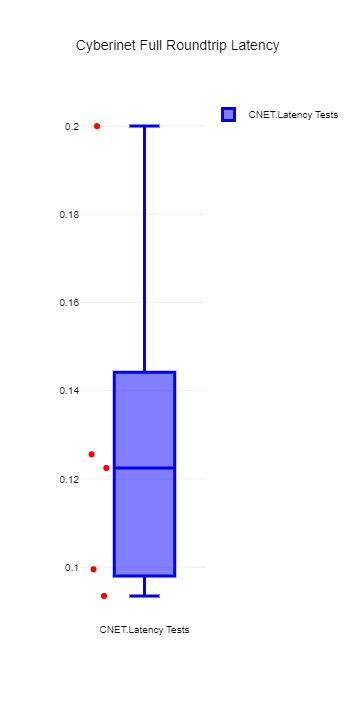
\includegraphics[scale=0.5]{newplot.png}
    \caption{First 6 Latency Tests of the Cyberinet (in seconds)}
    \label{fig:latencyTest1}
\end{figure}

Based on these tests, the average amount of time it takes for a gesture to be transmitted from the Cyberinet to Max, routed through the Max system, then out the speakers, and back into the microphone is just over 120 milliseconds. Excluding the outlier data point of 0.2\footnote{Seemingly randomly there would be a delay in one of the signals. This has not happened enough to be able to recreate and troubleshoot yet.}, that average drops to approximately 111 milliseconds. While significantly higher than a wired connection, this value is on par with the Bluetooth 4.2 specs\cite{btSpecs} of the ESP-32. When taking into account the data smoothing utilized within the Cyberinet, the parameters are adequate for most users.

\begin{figure}
    \centering
    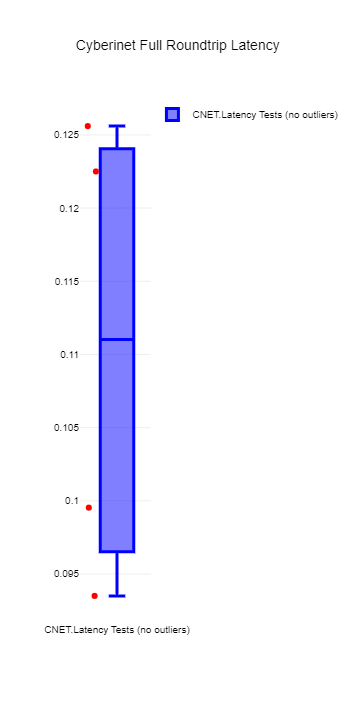
\includegraphics[scale=0.5]{newplot (1).png}
    \caption{First Latency Tests of the Cyberinet (excluding outliers)}
    \label{fig:latencyTest1}
\end{figure}

With an average round trip latency of 111ms, the Cyberinet's wireless capabilities are on par with most general Bluetooth headphones, which are generally acceptable for audio purposes. This value could be reduced in a couple of ways in future iterations. The method with the greates effect on latency be to convert the Cyberinet to a wired connection\cite{bluetoothLatency}, but this removes the ease of using Bluetooth. The main way to practically decrease latency in future revisions of the Cyberinet would be to upgrade the micro-controller from the ESP-32 to one which supports Bluetooth version 5.0 or newer. Version 5.0 can transmit twice as much data at once when compared to version 4.2\cite{btSpecs}. Some high-end devices have been measured at just over 30ms of latency\cite{bluetoothLatency}. Also keep in mind that this is the round trip latency. If a user is recording the data, or is otherwise only concerned with the transmission from the Cyberinet to the computer, then the Latency would be lower than 111ms.

\section{Max Programming}

To utilize the data being collected by the Cyberinet’s hardware, a collection of Max objects to help with the receiving and usage of said data have been developed. These allow the user to easily implement common effects and the mapping of gestures in Max without needing to worry about compatibility between the objects. It is important to mention that Max is a paid software. The CNET object and Cyberinet hardware components are all open source, however in order to create your own patches, the end-user will need to download the software. If saving patches is desired, then they must purchase a software license. Prior to utilizing the CNET objects, however the data being transmitted from the Cyberinet must be received, conditioned, and routed.

\subsection{Receiving \& Routing Data}

When implemented, the CNET objects are utilized to help receive and route the data within a Max patch. Once the sensor data has been transmitted from the Cyberinet utilizing the SerialBT.println() command in the Arduino code, it wirelessly moves into the connected computer. This connection utilizes Bluetooth, and can be easily managed in the Max software\footnote{Max version 8.5.x or newer is needed when working with the Cyberinet}. A single CNET object is utilized in order to help receive and parse the data stream from the Cyberinet. CNET.receive allows the user to easily configure which Bluetooth port to receive data from, then sends that data to various outlets for use in the Max environment. The internal workings of CNET.receive are shown in figure \ref{fig:cnet.receive}. There are three main subsections to CNET.receive that allow the Cyberinet to function.


\begin{center}
    \begin{figure}
        \centering
        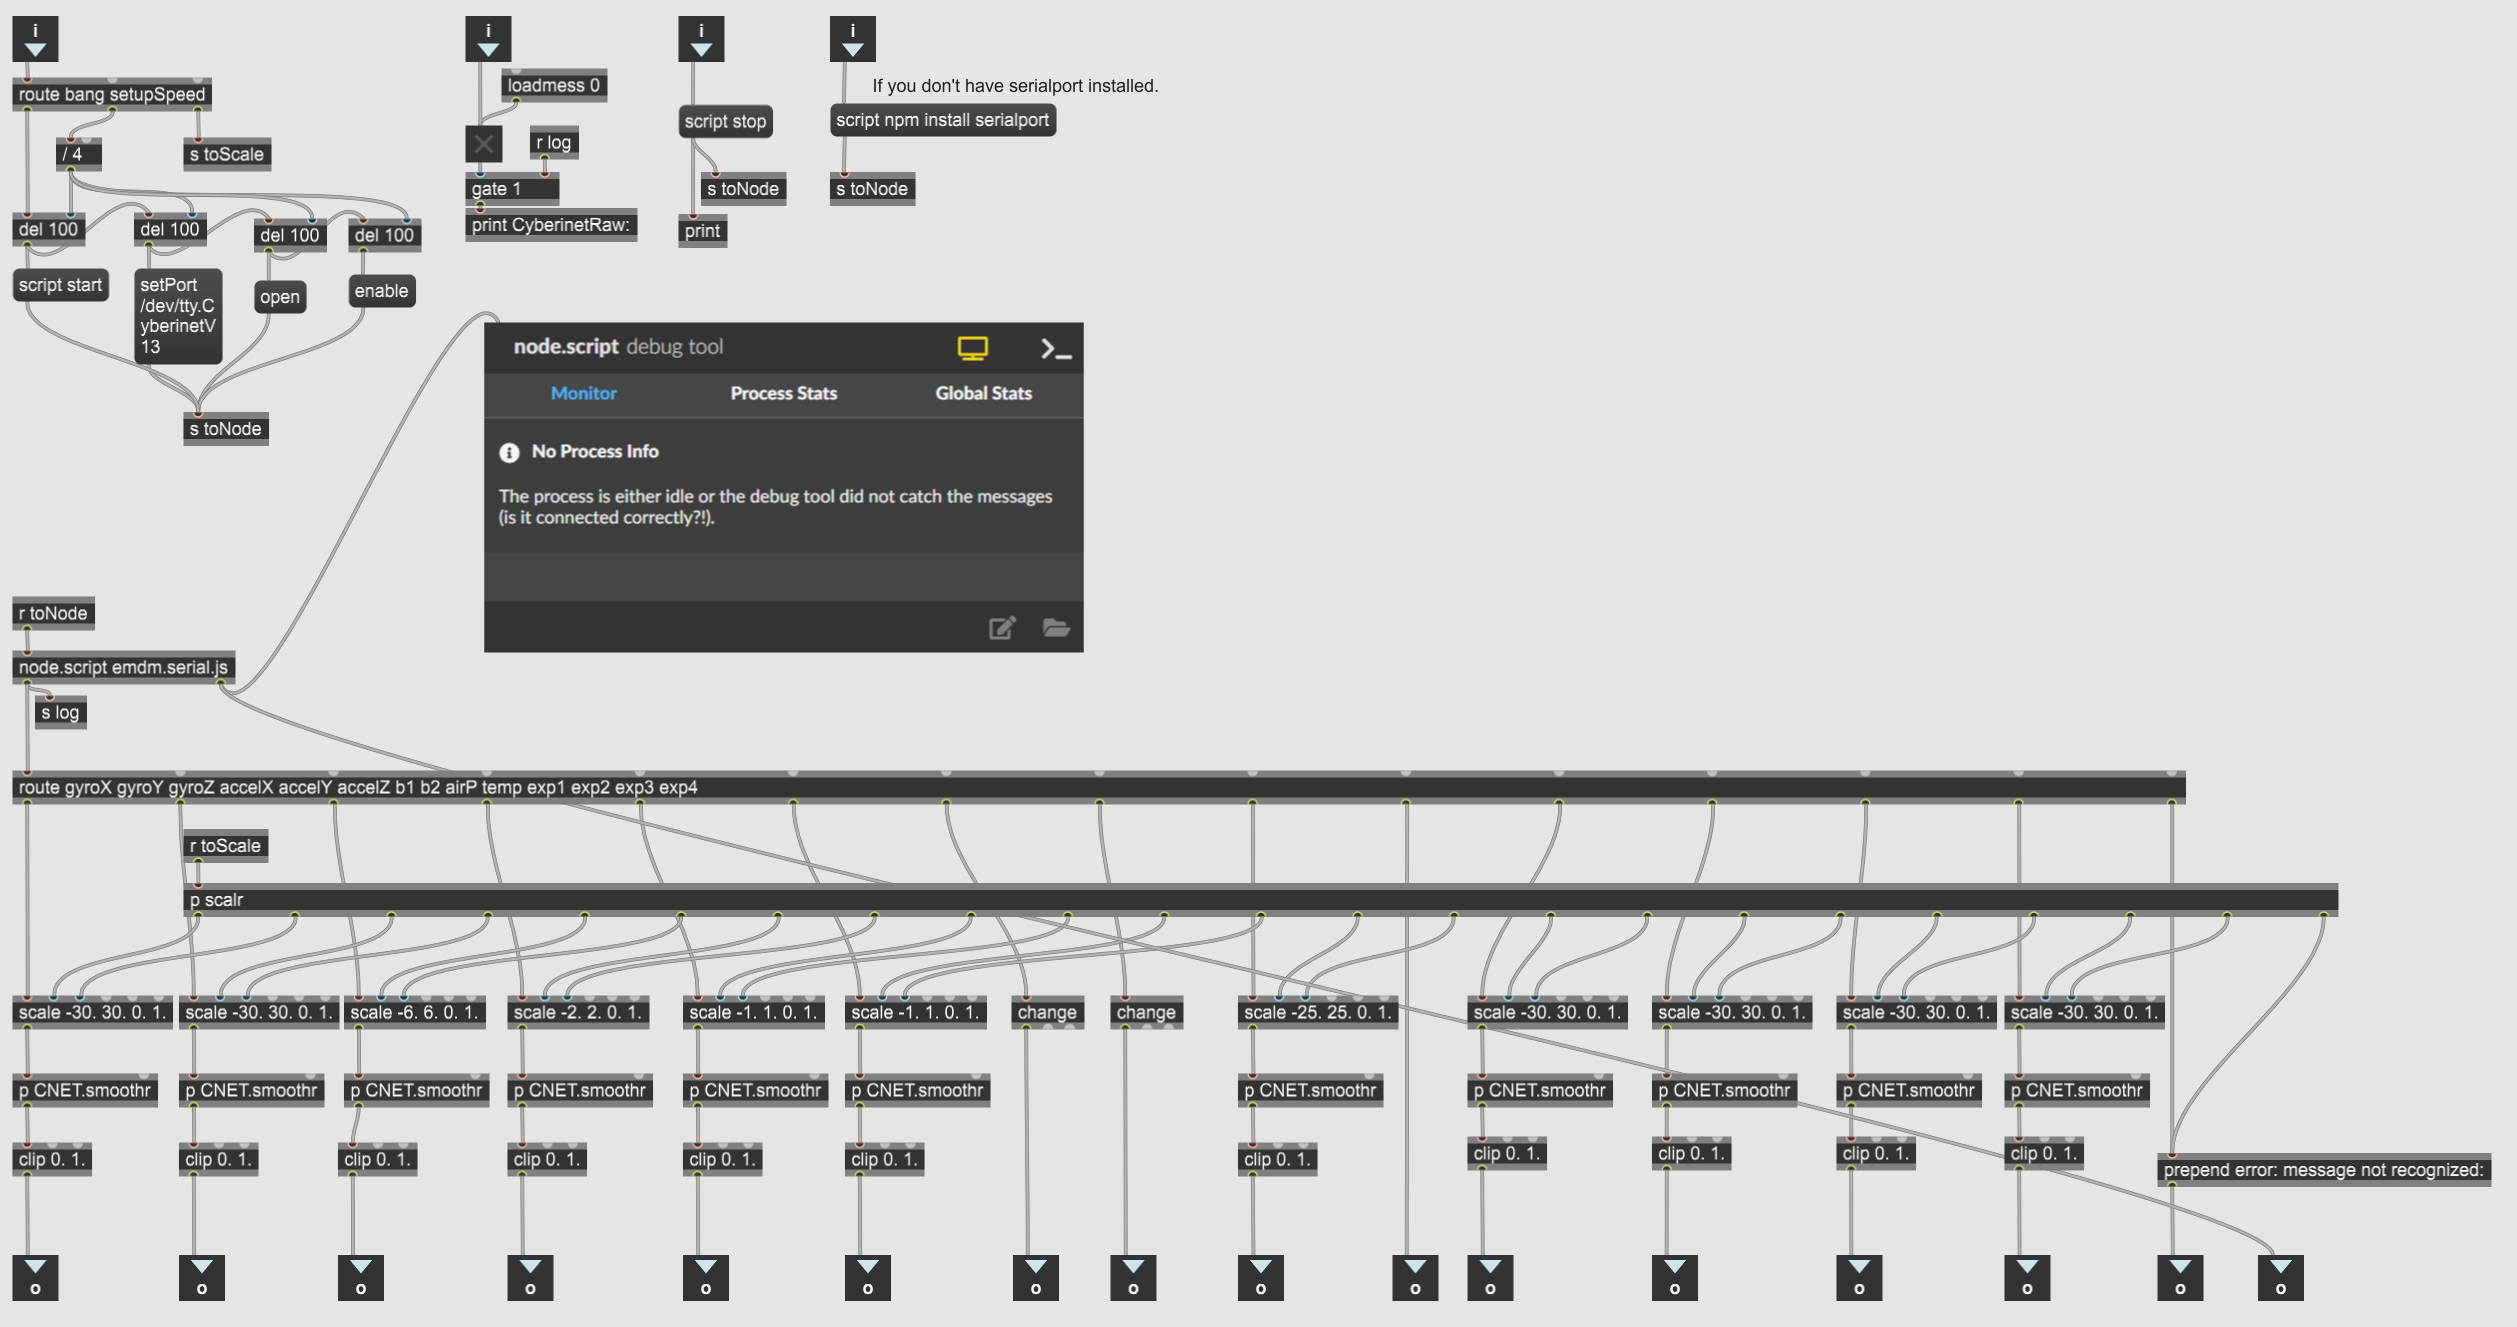
\includegraphics[scale=0.48, angle=270]{diagrams/maxPatches/CNET.receive.png}
        \caption{Inner workings of CNET.receive}
        \label{fig:cnet.receive}
    \end{figure}
\end{center}

The top section of figure \ref{fig:cnet.receive} shows the setup for beginning communications with the Cyberinet. A bang into the first inlet will begin running a node JavaScript file. This file helps max to communicate with the given port, respond to the data, and give feedback to the status of these communications in the Max console. The node.js debug tool can be helpful when monitoring the status of CNET.receive as well. Inlet two will toggle the printing of the raw data within the Max console in real time. This is useful, but can quickly take up computer memory due to the large number of data points being transferred. Inlet three stops communications when banged, and inlet four will install the various node dependencies when banged\footnote{This is only necessary if a computer does not already have these files installed. Once this has been done once, it is not needed unless moving to a new computer or if node was removed.}. 

When setting up communications, the initializing bang is actually achieving multiple steps. These were condensed in order to simplify and streamline the process for the user. A single bang will begin the node script, then set the desired port, open the port, and begin communications. A short delay is given between each of these steps. This is needed to give the computer enough time to respond to the messages. It is recommended to not change the delay time of these messages, but if needed the time can be adjusted with the control message "setupSpeed X" where X is the total delayed duration in milliseconds. that value is divided by four and equally applied to each internal delay object. All other control messages are used with CNET.rangeSet.

The middle section of the patch contains the node script\footnote{The full code of the node script is given in Appendix B} and a route object. The base for the node script came from a collection of objects created by LSU's Experimental Music \& Digital Media department. All this script does is receive the raw data on the indicated port and outputs it as a stream. The route object then parses the data based on the accompanying label from the Arduino code. Each label from figure \ref{fig:sensorLAbels} is utilized within the route object. The routing removes the label, outputting only the accompanying data values to their designated outlets. The data is then formatted for its final use outside of CNET.receive.

The final section of CNET.receive contains a large number of objects, but the process is repeated for the majority of the sensors. The sub-patch called "scalr" simply parses the lists from CNET.rangeSet, and outputs the value to the desired scale object below to adjust the internal scaling of values from the Cyberinet. These scale objects take the raw values from the Cyberinet hardware and proportionally adjust it to fit a range of 0-1. If a performer is generating a range of raw values that are too large or small for the desired effect, the internal scaling can be adjusted without altering the output range. The sub-patch "CNET.smoothr" is used for the final manipulation of the data, and is shown in figure \ref{fig:smoothr}. This object may potentially move into a more defined control object in the future, and is why it has a CNET name, despite not being a full object.

CNET.smoother takes incoming values and gradually slides between them instead of directly setting the values. This helps to make the effects sound continuous and minimize noise and popping. This defaults to being averaged over 20 data points. This value can be adjusted if needed, but experimentation is not recommended with this object. The second portion of this sub-patch compares the current smoothed data point with the previous one and calculates the difference between them. This value is then output back to the main patch, and clipped to the range of 0-1 to remove any outliers and avoid problems in the CNET effect objects. The result of this means that only when a sensor is actively picking up a gesture will it's data be utilized within Max. Using the gyroscope as an example, data will be output from CNET.receive while the instrument is actively rotating. When the performer is not performing a gesture, the values form a horizontal line when viewed through CNET.gestureVisualizer as in chapter 2.

Three sensors to not undergo this smoothing process due to their design. Both buttons only output values of 0 or 1. Smoothing those data points would remove the immediacy of a momentary switch. Instead, these values are output only when the button changes state. The only change to this data is that the binary data has been flipped from what was received from the Cyberinet. The hardware unit transmits a 0 when the button is pressed, but CNET.receive changes this to output a 1 when pressed and a 0 when released, allowing it to easily interface with Max's toggle object. This is the same for both buttons. The third sensor to not receive any smoothing is the temperature sensor. While these values could be smoothed, the difference calculations prove to be problematic in this situation. Generally speaking, any temperature fluctuations large enough to be interpreted as a gesture would be extremely uncomfortable for everyone in the performance space, assuming the performer is able to achieve in the first place. If the sensor was made more sensitive and respond to smaller fluctuations, then those changes cannot be detected by the audience as a gesture. To avoid all of these problems, the temperature data is output completely raw in degrees Celsius. This is the only value to not be conditioned in any way, as having the accurate temperature would be more useful than a 0-1 value in most situations when that sensor would be used.


\begin{figure}
    \centering
    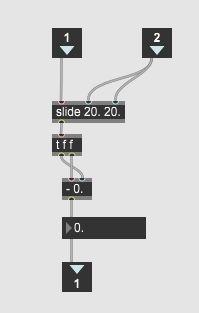
\includegraphics[scale=1.3]{diagrams/maxPatches/smoothr.png}
    \caption{Processing of smoothing and comparing the data stream within CNET.receive}
    \label{fig:smoothr}
\end{figure}

\subsection{CNET Objects}
The CNET collection of max patches works to interface the Cyberinet with Max in multiple different ways. Every object discussed as part of this collection has the prefix CNET, which is an abbreviation of the word Cyberinet. CNET can be broken into two main categories of patches based on how they interact with the Max Environment. Effect objects are largely commonplace audio effects that have been designed to work with the Cyberinet's data ranges. Control objects on the other hand are designed to manage the routing of data or provide feedback about the data being received by the various sensors.

Regardless of category, each CNET object has multiple inputs for those who want to utilize them to control the varied parameters for each object. These inputs are located immediately to the right of the main signal inlet, and are ordered to be a logical progression of controls from left to right. In the following section, each category of objects is listed with a short description. Each CNET object also has a detailed breakdown of its full control parameters, presets, and default values to show off the capabilities of the software both with and without a connected Cyberinet in the form of help patches\footnote{The CNET objects can be downloaded from \url{https://github.com/mbardin/Cyberinet}}.

\subsubsection{Effect Objects}

Effect objects are commonplace audio effects, with the exception of CNET.dmx. All of these objects are intended to take in data from the Cyberinet and utilize it to alter the performance environment. This is done through the processing of an audio signal. CNET.dmx achieves this goal by outputting values to control DMX lighting, and does not operate at the signal rate. Because of the wide variety of potential sound options with the Cyberinet, a handful of commonplace effects were chosen in order to help the user be able to easily create interesting effects that anyone with general musical knowledge would be able to easily implement. The current list of CNET effect objects is:

\begin{itemize}
    \item reverb$\sim$: A Schroder style reverb based on equations from CCRMA and John Chowning. This has a stereo output, and is similar to effects like JCReverb.
    \item monoReverb$\sim$: The same reverb above, but with a mono output instead of a stereo one.
    \item compressor$\sim$: A straightforward compressor based on the compressor objects created by Cycling74. This object has a stereo output.
    \item delay$\sim$: A single delay line using the tapin$\sim$ and tapout$\sim$ objects. The original signal is passed through, followed by the delay at a time set by the user.
    \item multDel$\sim$: Multiple delay lines utilizing 4 different tapout$\sim$ objects. Each one can have its individual output level set for unique mixing capabilities.
    \item feedbackDelay$\sim$: Identical to CNET.delay$\sim$, but with a feedback added for an echoing effect.
    \item vibDelay$\sim$: Functions similar to CNET.delay$\sim$, but includes a basic implementation of FM synthesis to adjust the pitch of the signal to be delayed. 
    \item karplusStrong$\sim$: Generates a plucked string effect using an incoming signal as the source material, and the Cyberinet to control the sound parameters. As the name implies, this uses Karplus-Strong synthesis.
    \item pitchShift$\sim$: Changes the pitch of an incoming signal. This can be controlled by MIDI  numbers or the 0-1 floating point range of the Cyberinet. Both the effected signal and the unaltered signal are output from this object.
    \item dmx: Converts data from the Cyberinet into control data for DMX lighting. This object is currently only compatible with the Chauvet DMX-AN 2 controller.
\end{itemize}


\subsubsection{Control Objects}

Control objects are used to specifically control or monitor the Max environment and other CNET objects. They do not alter signals in any way, but instead work to achieve tasks such as receiving data from the Cyberinet hardware, visualizing data, calculate latency, record and playback data in real time, etc. While the Effect objects are optional when using the Cyberinet and intended to be used in a creative context, the Control objects are more applicable in a large variety of utility settings and are highly recommended when developing a new composition. These objects include:


\begin{itemize}
    \item receive: This is the core of the Cyberinet's Max functionality. This object communicates with the hardware unit, parses, scales, and smooths all of the values before outputting each sensor's readings to a dedicated outlet. Values output from here are the change between data points, which helps to remove noise from the data and focus on the gestures.
    \item rangeSet: CNET.rangeSet can be used in conjunction with CNET.receive to adjust the internal value scaling from the Cyberinet hardware. If a performer's gesture data values are too small or large to be effective, this sets a new range for those expected values.
    \item record$\sim$: This object is used to record both the audio of the Cyberinet's performance, as well as the data points being output from CNET.receive. This object then saves the recordings as separate audio file and text data file. The data file also contains timings for playback.
    \item dataPlayback$\sim$: This object is used in conjunction with CNET.record$\sim$. The audio and text files created in that object are loaded into CNET.dataPlayback$\sim$ and started simultaneously. The timing values are used to schedule when the internal coll object reads each data point, allowing them to sync with the audio recording, thus replicating a physical performance.
    \item latency: Designed to test the latency of the Cyberinet within the Max environment. A sound is made on the Cyberinet's buttons, which trigger a noise gate. The resulting noise pulse is also played back and recorded. The resulting time between the press and the recorded pulse can then be analyzed to determine the full system Latency.
    \item  tuner$\sim$: This object functions like most other tuners available on the market. It will determine the pitch of an incoming signal and output the value as a signal. This is useful for checking and maintaining tuning within the Max environment, and for having the Max patch respond to certain pitches. This object requires a microphone be used to monitor the input as the ADC capabilities of the ESP-32 DEVKIT are unable to accurately execute this effect.
    \item gestureVisualizer: This object is the only CNET object with a dedicated GUI, and must be loaded into a bpatcher to be used as intended. This object receives incoming data from one of the Cyberinet's sensors and visually graphs the data points using Max's multislider object. Values are passed through the object regardless of the visualization state\footnote{This object was used for analyzing and categorizing the various gestures in Chapter 3.3.}.
    \item switch: CNET.switch acts similarly to the gate object within Max. It receives data from a Cyberinet sensor, and outputs a toggle when the changes exceed a sensitivity threshold. The object also has a cool-down timer to avoid undesired rapid switching. Both of these parameters are adjustable.
    \item test: This max patch is designed to test the functionality of the Cyberinet and CNET objects. It functions similarly to a help patch for the whole collection by receiving data and touting it to different effects utilizing a matrix interface. This is useful for debugging and prototyping
\end{itemize}


The main downside to the tuner object is that it requires the use of a microphone input to the computer. This is due to the limited ADC and Bluetooth capabilities on the Cyberinet's main ESP-32 Board. However, an unexpected upside to the object is it's pitch detection capabilities. The tuner object is able to detect both the musical pitch of the incoming signal, but also fine tuning in cents. Because this information is expressed both as a signal and in MIDI, it can be used to trigger a variety of other events in the max environment. While the list of possibilities is extensive, the idea of having the max patch harmonize with the Cyberinet is one application that has already been utilized in compositions for the instrument.

\subsubsection{Help \& Tutorial Patches}

Lastly, it should be mentioned that each CNET object also has a unique help patch associated with it\footnote{To access these help patches, insert the desired CNET object into a Max sketch, \\ then right click and select "Open XXX Help".}. The help patches are intended to help familiarize new users with the intended functionality of the objects, troubleshoot errors, and give various examples of their usage.

Each help patch is unique, depending on its functionality and intended usages, but all follow the same design template. Help patches give the title of the object, its version number and last edited date, and a description of what the object does. Below this, an interactive example is given that is unique to each object. Effect object help patches are used to alter the signal of a sound file, and Control object help patches are used to show off their specific functionality. Figures \ref{fig:compHelp1} and \ref{fig:switchHelp1} show an example of a help patch for both of these categories\footnote{All help patches have a mint-green color do differentiate them as help patches.}.

\begin{figure}
    \centering
    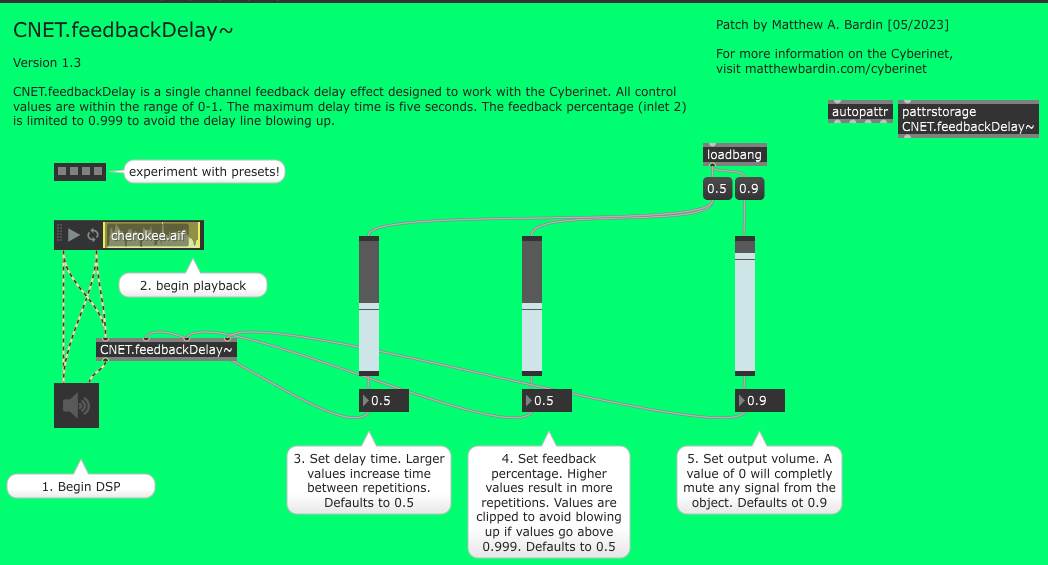
\includegraphics[scale=0.6]{diagrams/maxPatches/compressorHelp.png}
    \caption{Help Patch for CNET.compressor$\sim$}
    \label{fig:compHelp1}
\end{figure}

\begin{figure}
    \centering
    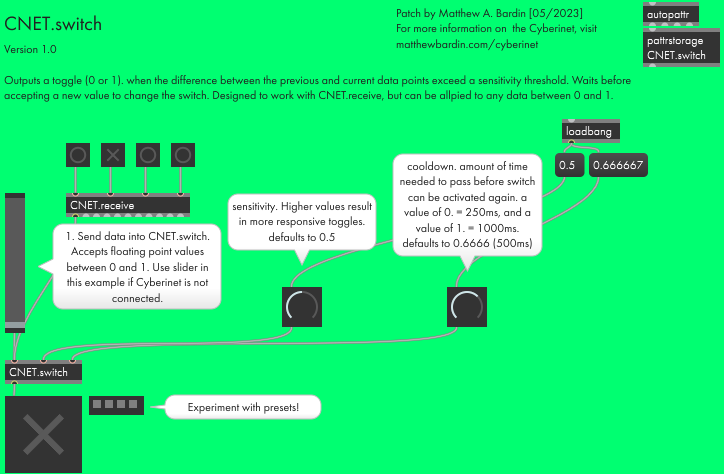
\includegraphics{diagrams/maxPatches/switchHelp.png}
    \caption{Help Patch for CNET.switch}
    \label{fig:switchHelp1}
\end{figure}

In addition to walking the user through how to setup and utilize the CNET object, each help patch contains between four and eight different presets. These are intended to show a variety of different parameter combinations, which reflect the capabilities of the object when used with the Cyberinet. Unless CNET.receive is required for the control object, it is not necessary to connect a Cyberinet to the computer in order to experiment with the help patches and their presets. Help objects where a physical Cyberinet connection is required are: CNET.receive, CNET.record$\sim$, CNET.rangeSet, CNET.test, and CNET.latency.


\chapter{Performing with the Cyberinet}
Now that we have looked into how the Cyberinet was created and programmed, it is important to discuss how the Cyberinet can be be used. This is not an extensive list of all potential uses, but rather the most common expected scenarios.

\section{The Cyberinet as a New Instrument}
The main intended use of the Cyberinet is as a new instrument as opposed to an add-on to a traditional B-flat Clarinet. The flexibility of utilizing the Cyberinet's sensor data can result in a large variety of potential sounds, even without the need for the traditional sound creation methods. A performer can utilize multiple Cyberinet sensors without traditionally playing the instrument, allowing the composer to explore new performance routes that may not be apparent if fully constricting themselves to the base Clarinet.

The cybernetic capabilities of the Cyberinet also allow for experimentation with the interplay between the acoustic performance and the electronic components. The modularity of the sensor routing within Max and the choice of expansion sensors also help to increase the creative sound possibilities. Early works for the Cyberinet are intended to focus more on the alteration of the Clarinet sound and controlling the Max environment, but more experimental CNET objects and expansion units are planned following the initial release.

So far, four unique compositions exist for the Cyberinet, and each composition features a different utilization of the sensors. \textit{Puzzle of a Park} utilizes the button expansion to control a Max patch. The end result is similar to a loop pedal. \textit{Ethereal Presence} utilizes accelerometer data to control harmonization and backing noise. \textit{ImprovImpisaImptionImpprovisation in Reverb} achieves a similar effect, but without notated gestures. \textit{Raindrops on a Tin Roof} utilizes all of the available sensors in version 1.3 to trigger sound file play back, processing of live and recorded sounds, and live lighting changes.

When mapping the gesture data, a composer is able to define specific movements to occur at specific moments within a performance. However, it is important to consider the perspective of the listener\cite{KvifteJenseniusDescription}. From this perspective, the listener will identify a physical gesture as well as the resultant musical sound, and make connection between. Regardless of the accuracy of this connection, it will happen to anyone paying attention to the performance. In a 2005 study, Wanderley et al. have found that:

\begin{quote}
    ... Clarinetists' ancillary gestures are not randomly produced or just a visual effect, but rather they are an integral part of the performance process\cite{wanderleyClarinetGesture2005}.
\end{quote}

The Cyberinet functions by taking these generally ancillary gestures, and translate them into the realm of audibility. In order to translate this clearly, the parameters must be clearly described to the performer with a  greater level of specificity than would be needed than if describing it to a listener\cite{KvifteJenseniusDescription}. Using Kvifte and Jensenius' paper as a methodology for describing these gestures, The Cyberinet exists squarely within the ratio level of measurement. This level of data is measured, with the distance of values determined, and an absolute zero value for each data exists, allowing for there to be 0 movement or airflow in the system. Being composed of specific values between 0 and 1, the data collected from the Cyberinet serves as a discrete input to the Max objects. Because of the modularity in the output, the sound production can be either continuous or discrete.

In practice, this results in a need for specificity in gesture notation to fully take advantage of the Cyberinet. A score needs to explain what, how, and when to perform the various gestures which generate the Cyberinet's data, as well as what the intended result is. Mappings can be static, where a gesture will remain fixed to a specific parameter. Variable mappings can be changed by the performer either as instructed or in a improvisation manner. Another option discussed by Kvifte and Jensenius is the system being able to learn and modify itself based on the gestures of the performer\cite{KvifteJenseniusDescription}. While highly cybernetic in concept, the current works for the Cyberinet do not utilize this method of mapping.

As a final note on specifying the gesture mapping, It is recommended to avoid mapping multiple gestures and sensors to a single effect at one time. This can easily obscure what the listener is perceiving as the gesture, leading to an ambiguous relationship. However, having multiple effects controlled by a single gesture is less problematic as it can create a more complex musical result to an initial gesture.

All of this leads into a still-evolving performance practice for the Cyberinet. The gestures being defined in the music help to build upon the structure of Clarinet performance to explore new directions by mapping the sensors and developing new intentional gestures to create previously un-heard sound capabilities. A process which is hindered by not viewing the Cyberinet as an entirely new instrument from a composition standpoint. The Cyberinet straddles a line between new and old. It works to bring new sounds and functionality to a traditional instrument with its own performance practice. Speaking purely practically, this brings about a certain mindset in the composer and performer when creating new music. To be the most effective, users should aim to create music with the electronic features in mind from the beginning, rather than working for an acoustic Clarinet with additional aspects added. 

The flexibility with which the Cyberinet can be utilized naturally leads to a large amount of exploration and improvisation. The audio effects provided with the CNET objects to allow for the user to easily begin creating their own sounds, however the Cyberinet is not limited to the use of CNET objects. By exploring which sensors are connected to different audio effects, the performer can create a large number of sounds based on a single performance gesture that they are already used to.

This modularity in signal processing is similar to the practice of using guitar stomp boxes to make a unique sound. While not physically similar, both systems allow for the quick customizable alteration of the instrument sound. When designing the initial CNET objects, effects present in effect pedals such as reverb, delay, filters, and tuners were used as an inspiration. From a pure performance standpoint, the Cyberinet can be utilized to significantly reduce the amount of equipment needed. The goal of this is to allow the performer to be able to create new sounds more freely, without the need to consciously manage equipment. This combined with the large variety of sound con control options is intended to be appealing for improvisers and performers who have a need to easily access a large variety of sound possibilities.

\section{Educational Tool}
Admittedly, at the time of writing the idea of utilizing the Cyberinet as an educational tool is still in its infancy. The concept came about when discussing the Cyberinet with various performers and graduate students during the LSU 2023 College of Music \& Dramatic Arts Research Expo. While not initially conceived in this manner, Implementing the Cyberinet as an educational tool can have interesting and long-reaching results for future Cyberinettists and electro-acoustic music performances. 

In short, these discussions focused on the motion (MPU-6050) and differential airflow pressure (SDP-31) embedded sensors. Looking at the accelerometer, the ability to determine the instrument's position could prove useful for new students learning the correct performance posture. This was the consensus of the small group of graduate researchers at the research expo. I felt that bringing up the positioning in early education may have a unique side effect that was not brought up in the casual discussion, that being a potential to apply Cybernetic or Deep Listening concepts to a performer's mindset from an early age.

If a performer is able to see clearly on a screen what their current position is and how to change that to improve their sound and posture, then they are learning how to observe and analyze their body and make changes to the system in real-time; creating a Cybernetic feedback loop\cite{WeinerCybernetics2019}. While beyond the scope of this document, this action brings to mind several concepts of the Alexander Technique\footnote{For more information on the principals of the Alexander Technique, visit \url{alexandertechnique.com}}. Specifically, the concept of self-awareness and adjustments to free the performer from habitual problems\cite{gelbBodyLearning2013}.

It was with this context of seeing and learning to be aware of the air pressure that the conversation led into the use of the SDP-31 in an educational sense. By giving real-time numerical or graphic feedback a performer could learn what values to expect when performing at various dynamics, the maximum and minimum amount of pressure difference they are able to create, as well as potentially identify any potential holes in their embouchure or leaky pads on their instrument. The same level of Cybernetic awareness and feedback apply to this sensor as well.

As additional expansions are created for the Cyberinet, their potential use in a pedagogical environment will need to be evaluated. Several of the expansions have potential for educational use, and more could be created following appropriate design and market research.

\chapter{Music Works Written for the Cyberinet}
As of the summer of 2023 a handful of musical compositions have been written that show off various features of the Cyberinet. Each of these compositions serve to utilize a specific subset of the available sensors, or show off a potential use case for the Cyberinet. At the time of writing, these are the only works written for the Cyberinet. As more works are written and explored, more uses and effects will be developed and refined.

\section{Gesture Notation for the Cyberinet}

The need for specific gestures is a necessity for the creation of meaningful Augmented Instrument functionality\cite{wanderleyClarinetGesture2005} \cite{miranda_Wanderley_instrumentControl_2006}, and for the performer to be able to Cybernetically perform. Without these, the Cyberinet's software mapping becomes harder to define in a consistent manner. Towards this, a small collection of gesture indicators are utilized within each of the musical scores. These symbols are only potential options for notating various movements and their effects within the music. Future compositions by other people will likely utilize their own unique notation.

These symbols are intended to clearly indicate a type of movement or action, and are explained in detail in the score's front matter. What is common between them though is that each symbol is visually unique, can indicate specific aspects of the gesture, as well as how long each gesture should occur for directly in the score. When applicable, the result of these gestures is also notated within the music.. 

% update as soon as final graphics are decided and in the scores this weekend.
Four different movement indicators were given for the seminal Cyberinet works. A variety was chosen in order to compare their effectiveness as a miniature experiment for future scores and studies. These indicators specifically indicate: 

\begin{itemize}
    \item Horizontal movement
    \item Vertical movement
    \item Rotation of the instrument
    \item Exaggerated breathing
    \item Button presses
\end{itemize}

The majority of the information from the indicators comes from the symbol present on each line. Horizontal movement is indicated with an H, vertical with a V, and breathing with a B. The type of line varies depending on the gesture. For example, in cases where the vertical movement should be repeated over a given amount of time, a wavy line is used. It should be noted that all of these indicators are symbolic of the gestures and not literal representations of the movements. Both options are valid when composing music for the Cyberinet, however due to the newness of the instrument, these symbolic representations are intended to encourage the performer to explore the functionality of the instrument and their own movements to achieve a result pleasing to them. 

\begin{figure}
    \centering
    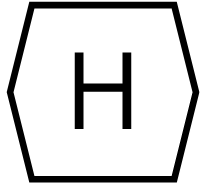
\includegraphics{h.png}
    \caption{Horizontal Movement Indicator}
    \label{fig:horMovement}
\end{figure}


\begin{figure}
    \centering
    \includegraphics{v.png}
    \caption{Vertical Movement Indicator}
    \label{fig:vertMovement}
\end{figure}

\begin{figure}
    \centering
    \includegraphics{b.png}
    \caption{Exaggerated Breathing Indicator}
    \label{fig:breath}
\end{figure}

Other symbols are used to specify a specific movement or action within the score. While kept simpler for the initial works, this approach could be applied to any potential physical gesture so long as the details of the gesture are communicated to the performer beforehand. The symbol shown in figure \ref{fig:rotateMovement} combines two potential gestures together. The arrow represents a quick counter-clockwise rotation of the Cyberinet, and the distinct note head, intended to look like a button, placed on the middle line indicates when a button should be pressed. While not always the case, these symbols are often utilized together in the scores discussed to indicate that either option may be used to achieve the same effect depending on the availability of the Button Expansion. In the works mentioned here, both gestures were used to progress the music into a different state.

\begin{figure}
    \centering
    \includegraphics{trigger.png}
    \caption{Rotational Movement \& Button Indicator}
    \label{fig:rotateMovement}
\end{figure}


When representing the gestures effect on the sound in the score, more graphic methods were used. These graphics can potentially prove difficult as the composer must balance the effect notation with readability in the score. For some effects, symbols were used to represent the effects, while others utilized a direct alteration to how the music appeared on the page.

The more exiting notations occurred within the score for\textit{Raindrops on a Tin Roof}, and were the most difficult to finalize. When a gesture results in the sounds having large amounts of reverb, the music is layered with a ghostly echo intended to represent the nature of the audio effect. The same is true for the heavily distorted images that still show the general shape of the music, but lose the finer details when distortion activates.

\begin{figure}
    \centering
    \includegraphics[scale=0.5]{verbbb.png}
    \caption{Notation of heavy reverb within\textit{Raindrops on a Tin Roof}.}
    \label{fig:verbbb}
\end{figure}

\begin{figure}
    \centering
    \includegraphics[scale=0.5]{deepfried_1684647887683.jpg}
    \caption{Notation of distortion within\textit{Raindrops on a Tin Roof}.}
    \label{fig:verbbb}
\end{figure}

Within \textit{Ethereal Presence}, abstract symbols are used because the sounds the effects being applied are not composed, but rather generated based on the performer's movements during the performance. which led to a more indeterminate way of notating repeating frequency sweeps and changing noise filters. The symbol representing repeated sweeping of signals is relatively self explanatory: the line represents the pitch of the synthesizer, but the noise symbol is more complex. For this symbol, the randomly placed dots represent the noise, while the thicker lines represent the filters changing which frequencies are heard.

\begin{figure}
    \centering
    \includegraphics[scale=0.5]{noize.png}
    \caption{Notation of noise filtering within \textit{Ethereal Presence}.}
    \label{fig:verbbb}
\end{figure}

\begin{figure}
    \centering
    \includegraphics[scale=0.5]{sweep.png}
    \caption{Notation of repeated synthesizer frequency sweeps within \textit{Ethereal Presence}.}
    \label{fig:verbbb}
\end{figure}


\section{Puzzle of a Park}
At its core, this work is the simplest of those written especially for the Cyberinet. \textit{Puzzle of a Park} functions similarly to a work written for a loop pedal, but without the pedal. The performer plays through the material from beginning to end, periodically pressing one of the two buttons on the button expansion\footnote{The specific button can be easily switched in Max to suit the performer's preference.}. That button will trigger the computer to record a microphone input into a buffer and the synchronized playback of all recorded buffers, resulting in the loop pedal effect. The rotation gesture mentioned previously was also programmed to achieve this goal in case a user does not have the Button Expansion. This functionality allows for multiple recordings to be saved and layered, much like loop pedals such as the Boss RC line of pedals. It also leads the user and audience member to see how the Cyberinet can be utilized to control sample recording and editing in real time. The user is also able to take advantage of the Cyberinet's wireless capabilities to easily perform in places where an excess of hardware and cables are not desired.

\begin{figure}
    \centering
    \includegraphics[scale=0.2]{diagrams/maxPatches/puzzlePresentation.jpg}
    \caption{\textit{Puzzle of a Park} Max Patch Performer View}
    \label{fig:puzzlePatchPres}
\end{figure}

\begin{figure}
    \centering
    \includegraphics[scale=0.25]{diagrams/maxPatches/puzzleRaw.jpg}
    \caption{\textit{Puzzle of a Park} Max Patch Full View}
    \label{fig:puzzlePatchRaw}
\end{figure}


When writing this work, the musical content was written as a quartet, with four unique voices rather than a single voice repeated several times. This allowed the musical content to flow and feel more organic once the final layer was added. Once the final loop had been completed, it was simply a matter of repeating the sequence of time signature and meter changes so that the score would form a repeating pattern. From there, each line was organized to be performed linearly over the course of five minutes. While possible with the Cyberinet and Max, this composition refrains from breaking down the recordings into smaller chunks and assembling them. Instead, the loop pedal approach is used to more clearly show the relationship between the gesture of pressing a button (or rotating the instrument) and the playback control.

When ordering the voices, \textit{Puzzle of a Park} begins with an internal harmony voice in order to set the overall texture and mood. It is then given the bass line support, another internal harmony, and the final melodic voice. Looking at the large-scale musical form of the solo, it can be described it as \emph{ABA'C} since the third and first voice are extremely similar in terms of structure and style and function; providing harmonic  and rhythmic content similar to a a horn part in a Sousa march. When combined, the first three voices provide a complete backing track to the main melodic line. Like fitting together, the pieces of a puzzle, it is this final line that helps to give context to all the phrases we have heard so far. Rhythms previously heard as down beats become upbeats, harmonic implications shift with the addition of new chord tones, and the texture is filled out to include the full range of the instrument.

When it came to gesture mapping, this piece utilizes the least of the works discussed in this chapter. In testing, it became a concern that the playback could potentially overpower the performer, so to mitigate that, the data from the air flow sensor was inversely mapped and applied to the make up gain parameter of CNET.compressor$\sim$, which all recorded sound files are sent through. This resulted in the make up gain level decreasing as the performer played more loudly. In general, this kept all four parts in relative balance, but would occasionally dip too much if the performer was playing too loud. However this is less of a gesture and more of a passive processing.

The other effect utilized in this work takes an incoming audio signal, analyzes its frequency compositing, and then filters noise at a low volume to result in a constantly shifting background sound that will always match the performance. When vertical bell movement is occurring, the sounds from this effect are mixed into the output, adding an additional level of texture to the performance, and further differentiating the recorded playback from the Clarinet timbre. Sounds are fed into the effect as more movement is detected, so the graphics change in order to indicate speeding up or slowing down. Because the result of the effect is fed into the recorded buffers, the movement is represented in the score when the loops begin repeating.

\textit{Puzzle of a Park} was premiered by Adam Cope on 04/18/23 at the LSU Digital Media Center Theatre and recorded later that summer.

\section{Ethereal Presence}
Ethereal Presence  begins to utilize the more complicated sensors present in the Cyberinet. The specified gestures all utilize the various movement sensors. Once received, the Max patch utilizes the values to control two different synthesizers, listed in figure \ref{fig:etherealSynths}. By utilizing the Cyberinet in this piece, focus is drawn the Cybernetic interactions with the audio synthesis. The rotation gesture was used to change the active synthesizer depending on the section of music.

\begin{figure}
    \centering
\begin{itemize}
    \item Pitch-shifted FM Synthesis that harmonize with the original Clarinet sound based on the vertical movement of the performer.
    \item Filtered pink noise using FFT bins that respond to the Horizontal position of the performer.
\end{itemize}
    \caption{Synthesizers used in Ethereal Presence}
    \label{fig:etherealSynths}
\end{figure}



The first synthesizer is a simple FM synthesizer with the goal of harmonizing with the soloist, and is the titular "Ethereal Presence". The goal is to make the tone as simple as possible, but with a large potential for timbral changes, which is why Max's built-in simpleFM object was utilized. The pitch of the incoming microphone signal is analyzed using CNET.pitchShift$\sim$, which is used to control the pitch of the FM synthesizer. The pitch will increase was the performer moves vertically, and decrease as they move downward. Accompanied by this is a more textural synthesizer designed to help support and fill out the atmosphere of the composition. This synthesizer outputs noise before being run through an FFT based filter created by Dr. Austin Franklin\cite{pnpMaxTools}. This filter takes the incoming noise and performs an FFT operation on it to determine the frequency content, then based on the values received from the Cyberinet, filters out certain frequency bins. The end result is a fluctuating cloud of noise that adapts its frequency range based on the Cyberinet's position. The range will increase with leftward movement, and decreases when moving to the right.


\begin{figure}
    \centering
    \includegraphics{diagrams/maxPatches/ethereal_pres.png}
    \caption{Ethereal Presence Performer View}
    \label{fig:etherealPerf}
\end{figure}

\begin{figure}
    \centering
    \includegraphics[scale=0.75]{diagrams/maxPatches/ethereal_raw.png}
    \caption{Ethereal Presence Full View}
    \label{fig:etherealRaw}
\end{figure}

When mapping gestures, general movements are indicated, but specific speeds are not specified. Aesthetically, this causes no two performances to harmonize in the exact same way each time, thus increasing the "etherealness" of the effect. While the Cyberinet is continually measuring the data, only one synthesizer is actively responding at ant given moment. Because of the value processing within CNET.receive, synthesizers will only be largely effected during and immediately following the gesture indicators in the score. The effects are alternated by quickly rotating the Cyberinet to trigger the CNET.switch object.

Because every performer is different and may be not achieve the full range of gestures to adequately control the synthesizers, CNET.rangeSet, was created to help mitigate that problem. CNET.rangeSet can adjust the scaling parameters within CNET.receive in order to make the results more or less sensitive. A smaller movement can result in a larger change in effects. It is recommended that this be utilized for calibration if an effect is not coming through as desired.

\textit{Ethereal Presence} was premiered by Adam Cope on 04/18/23 at the LSU Digital Media Center Theatre, and recorded later that summer.


\section{ImprovImpisaImptionImpprovisation in Reverb}
Similarly to \textit{Ethereal Presence}, \textit{ImprovImpisaImptionImpprovisation in Reverb} utilizes the gyroscope and accelerometer to control the computer processing. However instead of using the sensor data to control audio synthesis, this composition's algorithm controls multiple reverb and delay effects applied to the incoming signal from an onstage microphone.

\begin{figure}
    \centering
    \includegraphics{diagrams/maxPatches/imporvPres.png}
    \caption{ImprovImpisaImptionImpprovisation in Reverb Performer View}
    \label{fig:ImprovPres}
\end{figure}

\begin{figure}
    \centering
    \includegraphics{diagrams/maxPatches/improvRaw.png}
    \caption{ImprovImpisaImptionImpprovisation in Reverb Full View}
    \label{fig:improvFull}
\end{figure}

The specific control mapping for this composition are as follows: 

\begin{itemize}
    \item GyroX: gates signal to CNET.feedbackDelay$\sim$
    \item GyroY: feedback delay time
    \item AccelX: feedback delay percentage and output gain, and low harmonizer pitch
    \item AccelY: high harmonizer pitch
\end{itemize}

Of the four compositions existing for the Cyberinet, \textit{ImprovImpisaImptionImpprovisation in Reverb} is the only one that does not have a dedicated score. This was done to focus on the potential use of the Cyberinet as an improvisation tool. By utilizing the movement data from the Cyberinet, the patch encourages the performer to explore the performance space. In terms of the physical movements required to trigger the effects, they are closest to those used in \textit{Ethereal Presence}. However, the max patch for this composition contains three main processes controlled by the Cyberinet. 

The first is a reverb effect that is constantly applied to the sound. The amount of reverb present changed based on the horizontal movement of the performer. Following that, the patch automatically swaps between two different states if the player has not made a change in over two minutes. The first is a feedback delay where the delay time is controlled again by horizontal movement. Specifically, the audio signal for this process is only fed into the delay line when the instrument has been shaken or is otherwise actively moving horizontally. The final state of the patch takes the signal and using CNET.tuner$\sim$ and CNET.pitchshift$\sim$, creates triangle waves that harmonize above and below the performer based on their Y-axis movement (upstage vs downstage). can be interchanged through the same rotation gesture that is used in \textit{Ethereal Presence}, and are fed into additional, non-automated reverb effects as well as the same object which generates low-level background noise that is present in \textit{Puzzle of a Park}.

The Max patch for \textit{ImprovImpisaImptionImpprovisation in Reverb} utilizes a slightly different version of CNET.receive than all other works for the Cyberinet. This one is called CNET.receiveCaps. It is completely identical to CNET.receive in every way except that the labels used to route the sensor data all begin with capital letters. Because of the similarity with CNET.receive, this object is not discussed separately. It exists because the Cyberinet hardware used in the premiere of this work utilized an older version of the Arduino code that used capital letters instead of the camel-case that is conventional to modern coding. All versions of the Cyberinet following 1.2 use the preferred camel-case., and this version should be considered depreciated.

While not complex, this work emphasizes Van Nort's idea of a second-order level of gesture mapping\cite{vanNortMapping2007}. By being able to automatically or manually swap between the mapping states, the performer is able to further control and develop the relationship between sound and action. In a performance, the max patch will always default to the first state: the feedback delay. By having to move the instrument horizontally to activate the effect, the intention is that the listener will see the clear relationship between the two actions. Then, while not as drastic of an effect, the horizontal movement is utilized in the harmonization effect. The main control for the harmonizer is leaning back. Combined with a reverb effect that is always being affected by horizontal movement to act as an acoustic and gestural glue, the performer is able to create a clear relationship between the sounds and develop subtle variations between that relationship in a performance setting. I look forward to seeing future expansion on the idea of Second-Order gesture control with the Cyberinet in future compositions.

\textit{ImprovImpisaImptionImpprovisation in Reverb} was premiered on 05/01/2023 by Matthew A. Bardin in the LSU School of Music Recital Hall.

\section{Raindrops on a Tin Roof}
Of the debut compositions for the Cyberinet, \textit{Raindrops on a Tin Roof} is the most involved with the Cyberinet sensors. Contrasting from Mueller's usage of the SABRe in \textit{Sailing}, this composition utilizes all of the default sensors present in the hardware in some way. The inspiration comes from a short story written by myself in late 2022. The full text is provided in the appendices, but the general outline is as follows:

The main character (the Cyberinettist) is exhausted after a week of overtime at work and plans to enjoy a rainy weekend alone at home. During the storm, the protagonist falls asleep and wakes up to find the house completely dark and unfamiliar. Assuming the power has just cut out, they head to the basement to find some emergency lights when they discover an un-knowable eldritch abomination in the basement. Because of the un-knowable nature of the being, the protagonist forgets everything about it as soon as they run away. The end result is a bloodthirsty monster chasing the confused and terrified protagonist through the house and onto a rooftop veranda where the protagonist accepts their fate, and the monster has its dinner.

Formally, the music follows the narrative of the story, with ambient storm sounds and monster noises present in order to further enhance the theatrical elements of the work. These theatrical elements are further emphasized by the on-stage lights and optional smoke machine.

Positional information is used to control the live mixing of the pre-rendered tracks. These include:
\begin{itemize}
    \item Sounds created by the monster.
    \item Creaking floorboards and other ambience.
    \item Synthesizer Accompaniment.
    \item Narrator readings.
\end{itemize}


The airflow information is used to apply distortion to the accompaniment audio. As the performer's breathing intensity increases, so does the effect application. Unlike the other compositions discussed here, \textit{Raindrops on a Tin Roof} utilizes notated accompaniment within the score. This accompaniment is meant to represent the monster in the basement in a less literal sense than the ambient noises. These sounds were generated with the UVI 8-Bit Synth. The sounds were all pre-rendered using Studio One 6 Professional, and are intended to create a spooky, slightly incongruous sound when compared to the others present in the environment. The narrator files are a processed to add a distorted, low-fi sound to the voice to make it appear more ethereal in nature than clean recordings. 

The final two non-musical elements of this performance are a smoke machine and 2, or more, DMX-controlled lights. The smoke machine is not controlled by the performer, but the DMX lights are. The RGB lights are controlled by a mix of gyroscope and airflow values. The end result is the lights changing their green as the performer moves around the stage, and becomes more red as the performer breathes harder. The end result of all of these elements is a short theatrical performance entirely controlled by the Cyberinettist. In a traditional performance setting, these various elements would require multiple people or devices in order to pull off the same effects. By utilizing the Cyberinet in this context, a single person is able to control the entire tech aspects of the concert without having to directly manage each individual element; only their performance.

\begin{figure}
    \centering
    \includegraphics{diagrams/maxPatches/raindropspres.png}
    \caption{Raindrops on a Tin Roof Performer View}
    \label{fig:raindropsPres}
\end{figure}

\begin{figure}
    \centering
    \includegraphics[scale=0.6]{diagrams/maxPatches/raindropsRaw.png}
    \caption{Raindrops on a Tin Roof Full View}
    \label{fig:raindropsRaw}
\end{figure}

When mapping gestures, the score for \textit{Raindrops on a Tin Roof} contains the most specific level of gesture notation. In general, three gestures are utilized outside of the natural gestures of a performance. These are: 

\begin{itemize}
    \item Exaggerated movement
    \item Exaggerated breathing
    \item Movement between stands on stage
\end{itemize}

When notating this work, one concern was clutter on the page. to help minimize this, the score was printed on tabloid (11inx17in) sized paper\footnote{The score has been scaled down to fit within this document.} in order have more physical space on the page. 

The final gesture indicator was to move to a different location on the stage. This was indicated with text at the appropriate place on the score. No physical stand transitions occurred before the end of a page, and this proved effective is sending a large number of values to all of the sensors at once, resulting in a more drastic effect to mirror the sudden physical movement.

\textit{Raindrops on a Tin Roof} was premiered by Adam Cope on 04/18/23 at the LSU Digital Media Center Theatre, but did not include the optional smoke machine.



\chapter{Conclusions} 

\section{User Opinions}

As previously stated, being a new augmented instrument, the aforementioned four works are the only compositions for the Cyberinet at the time of writing. To better inform future revisions and compositions, the two performers who premiered the above works were asked a series of questions following their usage of the Cyberinet. These questions were:

\begin{itemize}
    \item Question 1: How easy or difficult was it to implement the Cyberinet into your normal performance routine?
    \item Question 2: What was your favorite and least favorite part about working with the Cyberinet? 
    \item Question 3: How confident do you feel in being able to remove or add the Cyberinet to your Clarinet in a performance setting?
    \item Question 4: How confident do you feel in being able to work with the Cyberinet's software capabilities to create unique sounds?
    \item Question 5: What thing or things did you dislike, or would change, about the Cyberinet?
\end{itemize}

In order to protect the identity of the performers, they are referred to by number. Performer 1's responses are shown below: % Adam

\begin{itemize}
    \item A1: It's very straightforward, akin to switching Clarinets, as one would for an orchestra performance. Just switching out the barrel and adding the thumb rest attachment it all it takes to incorporate the Cyberinet into my performance routine.
    \item A2: My favorite part about working with the Cyberinet has been exploring how to incorporate the movement sensors into my performance. Normally the way you move doesn't directly affect the sound you're putting out, so it's interesting to see the new ways in which I can express myself! My least favorite part is probably th
    \item A3: Assuming future versions will be able to connect and transmit data more reliably, I would say I'm very confident in adding and removing the Cyberinet.
    \item A4: As someone who is not well versed in Max, I'm not confident in my ability to create new sounds on the software side of things. As a performer first, I feel confident in my ability to use the equipment, but not necessarily to create for it.
    \item A5: The only thing I would change is to reverse the ports that connect the thumb rest buttons to the barrel. Right now, the connecting cable kind of sticks into the player's right hand a bit, but I imagine that would be a non issue if the ports were flipped to the opposite side.
\end{itemize}


The below responses belong to performer 2. % Me

\begin{itemize}
    \item A1: It was simple enough to implement, however there was a bit of a learning curve needed to reliably connect the device to the computer. Once I had the steps memorized it was reliable and simple to use.
    \item A2: My least favorite part was having to install all of the various drivers the first time. My favorite part was exploring with the gyroscope sensor and a reverb effect. the result was fun and intuitive.
    \item A3: I've already mentioned the issues in setting up the Cyberinet at the beginning, but being able to simply turn off the power and utilize the instrument completely acoustically as needed. This is easier than removing the unit.
    \item A4: I am already familiar with the Max environment so I feel that I could easily set up a lot of scenarios with the Cyberinet without much difficulties, but more reference material would be helpful. 
    \item A5: Other than the things I've already mentioned, I suppose I'd say relocating the port on the Button Expansion to a better location and potentially reducing the size of the main unit a little. It isn't too large, but a think a little smaller would be easier to work with.
\end{itemize}

In general, the people using the Cyberinet find it easy to implement both in terms of hardware and software, but mainly request various tweaks to different aspects of the design. Since these questions have been asked, the thumb rest has been altered to resolve this problem and the Max objects have also been optimized for simpler connections and management, but other improvements will have to wait until the second iteration.

\section{Future Development}

While the Cyberinet has been created to achieve a set of goals, it has always been designed to be continually expanded past its initial iteration. This includes both expanding the various elements of the hardware and software, but also further refining and improving the current materials. In terms of expansions, the main focus of development is to the CNET objects and expansion units.

In regards to the CNET objects, the current version is a collection of common audio effects and tools. While effective, they only show a small slice of the possibilities of utilizing the Cyberinet in Max. Future CNET objects are intended to both increase the amount of common effects, but explore more unique effects and timbres. The main focus of these new objects are those which generate their own audio based on the Cyberinet values, an aspect minimally present in the current CNET version.

Also in the realm of programming, a few improvements to the Arduino code running on the ESP-32 are planned as well. In the current software version, the button expansion LED's are only illuminated when the buttons are pressed. However they are wired independently of the switches on the expansion. In future versions, the ability to control these LED's via the Max software is planned. This would result in being able to provide another method of feedback to the performer based on the state of the Max patch.

It is also intended to move the Cyberinet from utilizing Max exclusively, to utilizing OSC to allow for additional programs to easily utilize the data. This will be achieved in multiple steps. The first is the development of a Max object that packages and outputs the data as an OSC message, which will be the main method of utilizing the feature. Future versions of the Arduino code will transmit data already in this format, but the Max object will allow older units to achieve the same functionality.

Version one of the Cyberinet is currently only compatible with Mac systems. Similar to increasing the software compatibility with OSC messages, the ultimate goal is to have the system compatible with Windows systems, but will enquire a mixture of adjusting the serial protocol on the physical units and the CNET.receive object.

In terms of hardware, the aforementioned joystick and microphone expansions are planned be completed over the fall and winter of 2023. Additional plans for the following sensors to be released following those have also been made, but active development has not yet begun at the time of writing.

\begin{itemize}
    \item Pressure Sensor: responds to varying pressure on the instrument's keys. Needs special mounting of Force-Sensitive-Resistors, as well as doughnut-shaped FSRs.
    \item Pitch Detection: Works like the tuner software object. This will display tuning information and transmit pitch information to the computer. Needs hardware with adequate Analog-to-Digital Conversion.
\end{itemize}

At the time of writing, the Cyberinet is only available for B-flat soprano Clarinets. While this is the most commonly found Clarinet, it represents only a fraction of the total woodwind family. In the future, plans to adapt the hardware case to fit different instruments will allow for the Cyberinet to be utilized in an exponentially larger number of scenarios. First, adapting the unit for the A Clarinet and Bass Clarinets. At this time there are no plans to expand to an E-flat Clarinet due to the limited space to attach electronic components. Following the Clarinet expansions, ideas for compatibility with Saxophones and Flutes are being discussed, but require more planning in order to make functional units.

Currently the programmable LED within the Cyberinet is only able to communicate when a data value is being transmitted. Future plans for the software, specifically the node script, will allow for the user to send information to the Cyberinet, which can then be relayed using this on-board LED.

The final minor element of hardware that will be explored are improving cable management and stress relief within the unit. This is intended to improve the functionality of the ports and reduce the amount of glue holding the components into the hardware case. 

As the design continues to be refined and expanded, plans for a Cyberinet "Pro" are being made. This involves moving away from the OEM components in order to create a more condensed hardware unit with potentially higher quality components. This would drive the price to produce a unit up however, which is why this is intended to be a second version of the device, similar to companies like Apple releasing a regular, Air, and Pro version of their Macbook computers.

\section{Conclusions}

The Cyberinet is a new digital augmented instrument designed to bring a large variety of audio production and control capabilities to the Clarinet. this control can be applied passively by analyzing the movements of the instrument, or specifically controlled through intentional gestures. This data is collected through a collection of sensors embedded within the instrument and wireless transmitted to a nearby computer, which is the device handling the control based on the received data.

Overall the Cyberinet has proved effective in a variety of performance scenarios, and is overall easy to implement following the initial setup. In terms of improvement, Focuses on simplifying the initial instillation to not require node.js as well as reducing latency are being made in order to improve the user experience.

While discussed here, a more concrete methodology for gesture notation with the Cyberinet would also greatly benefit future compositions for the instrument, but overall the basis for being able to easily and quickly implement electronic control to an otherwise standard Clarinet has been developed with the Cyberinet, and the main focus of future development is the creation of new music, as the creation of music will continue to highlight the strengths and weaknesses of the current iteration.

%% The command ``\appendix'' switches into appendix-mode, meaning that subsequent ``\chapter'' commands will instead produce appendices.
\appendix

\chapter{Cyberinet Hardware Designs}
This appendix contains images for all of the 3D models and PCBs used within the Cyberinet. It also contains close-up images of each of the individual OEM sensors.

\section{3D models}
Below are all of the 3D models utilized to 3d print the case and accessories of the Cyberinet

\subsection{Main Body}

\begin{figure}
    \centering
    \includegraphics[scale=0.4]{diagrams/3D Models/Cyberinet main case 3d.png}
    \caption{Main Unit of the Cyberinet from various angles}
    \label{fig:main3D}
\end{figure}



\subsection{Button Board Thumbrest Mount}

\begin{figure}
    \centering
    \includegraphics[scale=0.8]{diagrams/3D Models/thumbrestPic.png}
    \caption{Button Board Thumbrest Mount in 3D printing software}
    \label{fig:thumbrest}
\end{figure}



\section{PCB Diagrams}
Below are the PCB diagrams for the Cyberinet. Main unit and Button Expansion


\begin{center}
\begin{figure}
    \centering
    \includegraphics[scale=0.3]{diagrams/PCBs/mainBoard.png}
    \caption{Cyberinet Main Unit PCB}
    \label{fig:mainPCB}
\end{figure}
\end{center}



\chapter{Cyberinet Software Components}
This appendix contains all of the Arduino code flashed to the Cyberinet. (Version 1.3), as well as screenshots of the various max patches and objects included in the software bundle.

\section{Arduino .ino Code}

Below is the .ino code that is running on the ESP-32 micro-controller. This code was developed using the Arduino IDE and coding language.

\begin{lstlisting}[language=Arduino] 
/* Micro Controller Code for the Cyberinet Version 1.3, Code may be used or reworked with Attribution.
   Code and Other Matierials for the Cyberinet can be found at https://github.com/mbardin/Cyberinet
   Code and Other Marerials made  by Matthew A. Bardin [2023] (https://matthewbardin.com)*/

//libraries to include
#include <SparkFun_SDP3x_Arduino_Library.h>
#include<Wire.h>
#include <BluetoothSerial.h>
#include <MPU6050.h>

BluetoothSerial SerialBT;
MPU6050 mpu;
SDP3X airFlow;

const int pwrLED = 2; 
const int msgLED = 4; 
const int button1 = 12;
const int button2 = 14;
const int b1LED = 26;
const int b2LED = 27;
const int expPin1 = 33;
const int expPin2 = 32;
const int expPin3 = 35;
const int expPin4 = 18;
const int MPU_ADDR = 0x68; 
int16_t AcX, AcY, AcZ, GyX, GyY, GyZ; 
float rotX, rotY, rotZ, gForceX, gForceY, gForceZ; 
int button1State = 1;
int button2State = 1;
int exp1State = 0;
int exp2State = 0;
int exp3State = 0;
int exp4State = 0;

void setup() {

  pinMode(pwrLED, OUTPUT);
  pinMode(msgLED, OUTPUT);
  pinMode(button1, INPUT_PULLUP); 
  pinMode(button2, INPUT_PULLUP);
  Serial.begin(115200);
  SerialBT.begin("CyberinetV13"); 
  delay(1000); // pause before checking
  gyroStartup();
  airflowStartup();
  startLights();
}

void loop() {
  get6050();
  getButtons();
  getExp();
  getAir();
}

void get6050() {
  Wire.beginTransmission(MPU_ADDR);
  Wire.write(0x3B); 
  Wire.endTransmission(true);
  Wire.requestFrom(MPU_ADDR, 6); 
  while (Wire.available() < 6);
  AcX = Wire.read() << 8 | Wire.read(); 
  AcY = Wire.read() << 8 | Wire.read(); 
  AcZ = Wire.read() << 8 | Wire.read(); 
  Wire.beginTransmission(MPU_ADDR);
  Wire.write(0x43); 
  Wire.endTransmission();
  Wire.requestFrom(MPU_ADDR, 6); 
  while (Wire.available() < 6);
  GyX = Wire.read() << 8 | Wire.read();
  GyY = Wire.read() << 8 | Wire.read();
  GyZ = Wire.read() << 8 | Wire.read();
  rotX = GyX *  0.007633587786; 
  rotY = GyY *  0.007633587786;
  rotZ = GyZ *  0.007633587786;
  gForceX = AcX * 0.00006103515;
  gForceY = AcY * 0.00006103515;
  gForceZ = AcZ * 0.00006103515;
  digitalWrite(msgLED, HIGH); 
  SerialBT.print("gyroX "); 
  SerialBT.println(rotX); 
  SerialBT.print("gyroY "); 
  SerialBT.println(rotY); 
  SerialBT.print("gyroZ "); 
  SerialBT.println(rotZ);
  SerialBT.print("accelX ");
  SerialBT.println(gForceX);
  SerialBT.print("accelY ");
  SerialBT.println(gForceY);
  SerialBT.print("accelZ ");
  SerialBT.println(gForceZ);
  digitalWrite(msgLED, LOW);
}

void getButtons() {
  button1State = digitalRead(button1);
  button2State = digitalRead(button2);
  digitalWrite(msgLED, HIGH); 
  SerialBT.print("b1 ");
  SerialBT.println(button1State);
  digitalWrite(b1LED, button1State); 
  SerialBT.print("b2 ");
  SerialBT.println(button2State);
  digitalWrite(b1LED, button2State);
  digitalWrite(msgLED, LOW); 
}

void getExp() {
  exp1State = digitalRead(expPin1);
  exp2State = digitalRead(expPin2);
  exp3State = digitalRead(expPin3);
  exp4State = digitalRead(expPin4);
  digitalWrite(msgLED, HIGH);
  SerialBT.print("exp1 ");
  SerialBT.println(exp1State);
  SerialBT.print("exp2 ");
  SerialBT.println(exp2State);
  SerialBT.print("exp3 ");
  SerialBT.println(exp3State);
  SerialBT.print("exp4 ");
  SerialBT.println(exp4State);
  digitalWrite(msgLED, LOW);
}
void getAir() {
  float diffPressure; 
  float temperature; 
  airFlow.readMeasurement(&diffPressure, &temperature);
  digitalWrite(msgLED, HIGH); 
  SerialBT.print(F("airP ")); 
  SerialBT.println(diffPressure, 2); 
  SerialBT.print(F("temp "));
  SerialBT.println(temperature, 2);
  digitalWrite(msgLED, LOW); 
}
// startup functions
void gyroStartup() {
  Wire.begin(21, 22, 100000);
  Wire.beginTransmission(MPU_ADDR);
  Wire.write(0x6B); 
  Wire.write(0);     
  Wire.endTransmission(true);
  SerialBT.println("MPU-6050 Setup Complete");
}

void airflowStartup() {
airFlow.stopContinuousMeasurement();
 if (airFlow.begin() == false){
  SerialBT.println(F("SDP31 not detected.));
  while (1);
  }
airFlow.startContinuousMeasurement(true, true); 
SerialBT.println("SDP31 Setup Complete");
}

void startLights() { 
  digitalWrite(pwrLED, HIGH);
  digitalWrite(msgLED, HIGH);
  delay(500);
  digitalWrite(msgLED, LOW);
  delay(500);
  digitalWrite(msgLED, HIGH);
  delay(500);
  digitalWrite(msgLED, LOW);
  delay(1000);
  digitalWrite(msgLED, HIGH);
  delay(1000);
  digitalWrite(msgLED, LOW);
}
\end{lstlisting}


\section{CNET Max Objects}
This section discusses each of the CNET objects that were created with the intention of interfacing with the Cyberinet. With the exception of CNET.receive, these are smaller objects designed to easily implement the Cyberinet into some of the common audio effects the user is likely already implementing in Max. Because of how CNET.receive works, these objects are not required to utilize the Cyberinet, but are recommended for people learning how to work with Max or the Cyberinet for the first time.

Each object listed here also has a help patch which walks the user through setup and adjusting the values for that object. The help patches do not need the Cyberinet to be connected to work, and contain 3 different presets to show a variety of sound options. All inlets for these object utilize a 0-1 floating point number for parameter control. Default values for these inlets are all given in the help patches.

\subsection{Functional Objects}
These objects serve to increase the functionality of the Cyberinet and do not alter sound sources or control other objects.

\subsubsection{CNET.receive}
This is the only required object in the CNET collection. This object is responsible for setting up communications with the Cyberinet, parsing the data, and outputting it to the various outlets. Each sensor on the Cyberinet has a dedicated outlet, so connecting to each outlet will always relay the same sensor. The outlet order is given below.

\begin{enumerate}
    \item gyroX
    \item gyroY
    \item gyroZ
    \item accelX
    \item accelY
    \item accelZ
    \item b1
    \item b2
    \item airP
    \item temp
    \item exp
    \item errorMsg
\end{enumerate}

The final outlet will output an error indicating that CNET.receive received a message it did not recognize, as well as the error causing message.

To establish communications, bangs and toggles are utilized in order to simplify the interface. The user inputs a bang to the first inlet to start the script and list the available ports. When paired to the computer via Bluetooth, the Cyberinet will appear on the list of available ports. The user can then set the port by filling in the message box connected to inlet 2, and receive communications with a bang to the third inlet. Inlet 4 will stop all communications. The process will have to be repeated to initialize them again, and a bang to inlet 5 will install necessary node package manager dependencies and drivers the first time a computer is utilizing the Cyberinet.

The Node script and functionality comes from a package created by the LSU Experimental Music \& Digital Media department, and the JavaScript code for this is shown below in its entirety.

\begin{lstlisting}[language=JavaScript] 
const path = require('path');
const Max = require('max-api');
const { SerialPort, ReadlineParser } = require('serialport')
const baud = 115200;
let devicePort = '/dev/tty-CyberinetV13';
let port, availablePorts;
let parser = new ReadlineParser();
Max.post(`Loaded the ${path.basename(__filename)} script`);
Max.addHandler("echo", (msg) => {
	Max.outlet(msg);
});
Max.addHandler("portlist", () => {
  SerialPort.list().then((ports)=>{
    Max.post("Ports: ", ports);
    console.log(ports);
    availablePorts = ports;
  });
});
Max.addHandler('setPort', (port) => {
  devicePort = port;
})
Max.addHandler('open', () => {
  port = new SerialPort({
    path: devicePort,
    baudRate: baud,
  }, function (err) {
    if (err) {
      return console.log('Error: ', err.message);
    }
  })
})
Max.addHandler('enable', () => {
  Max.post('Serial Receive Enabled');
  port.pipe(parser);
  parser.on('data', (cyberData)=>{
    let cyber = cyberData.split(" ");
    let sensor = cyber[0];
    let value = parseFloat(cyber[1]);
    Max.outlet(sensor, value);
  })
})
Max.addHandler('send', (data) => {
  port.write(data, function(err) {
    if (err) {
      return console.log('Error on write: ', err.message);
    }
    console.log('message written');
  })
})
\end{lstlisting}

In short, after setting up the port communications, this code will identify the label:value pair and output them separated by a space via the outlet in the Node object. From there, a Max route object separates the values to different outlets based on the labels shown above. Values are scaled to fit a range of 0-1 where appropriate.

\subsubsection{CNET.rangeSet}
Used for adjusting the value scaling within CNET.receive. This object is used to fine tune the ranges expected for a performer with their Cyberinet unit. Maximum and minimum sensor values can be determined by looking at the Max terminal when the raw outputs are being displayed. Ranges are set to a specific sensor utilizing the same labels as those used in CNET.receive. Setting the sensor label with a message or sending a bang to the first outlet will trigger a list to be output from this object.

Within CNET.receive, an additional route and a handful of unpack objects are used to properly apply the data. All values leaving CNET.receive are still mapped to a range of 0-1 after this new scaling occurs.

\begin{figure}
    \centering
    \includegraphics{diagrams/maxPatches/CNET.rangeSet.png}
    \caption{CNET.rangeSet.maxpat}
    \label{fig:CNET.rangeSet.maxpatch}
\end{figure}

\subsubsection{CNET.latency$\sim$}
Used to calculate the latency between the Cyberinet detecting a sensor value change on the hardware, and that change being reflected in the Max environment. To achieve this, a microphone is needed. 

To test the latency, first you must connect the Cyberinet using CNET.receive, and ensure that the Button expansion is connected. 

Using the patch, a sound file is recorded. One channel of the stereo file records the sound of a button clicking on the Cyberinet. This button press is used to generate a pulse of white noise on the second channel.

The recordings are then compared to determine the time between the real-world action and the software response which is represented in milliseconds for the user. Large objects located between the computer and the Cyberinet may negatively affect the latency.

\subsubsection{CNET.tuner$\sim$}

This object is a simple tuner based off of the retune$\sim$ object native to Max. It receives a signal from an external microphone and outputs both the closest MIDI pitch and frequency of the sound. These values are output as signals. In this version of the Cyberinet, it must be located in the Max software as the ESP-32's ADC's are not powerful enough to run a tuner along with everything else. It is recommended for both tuning purposes, as well as pitch identification purposes. 

\begin{figure}
    \centering
    \includegraphics[scale=0.2]{diagrams/maxPatches/CNET.tuner~.png}
    \caption{CNET.tuner$\sim$.maxpat}
    \label{fig:CNET.tuner~.maxpat}
\end{figure}
 

\subsubsection{CNET.click$\sim$}
This object is able to receive a BPM value and outputs both a bang in Max, but also sends an audio signal click. This signal can be used by connecting a [receive$\sim$ click] to the desired output. For the compositions discussed in this document, the click track was always connected to channel 3 of the audio interface.

\begin{figure}
    \centering
    \includegraphics[scale=0.2]{diagrams/maxPatches/CNET.click~.jpg}
    \caption{CNET.click$\sim$ max patch}
    \label{fig:CNET.clickPAtch}
\end{figure}

\subsubsection{CNET.pan}
I was unsure about which section to place this object in. I chose its ultimate placement here as the object is not directly changing the sound, but rather it receives data to control the stereo panning of a signal.

\subsubsection{CNET.dmx}
This object functions to allow the Cyberinet to control DMX lighting with its various sensors. Note that this will not work with every DMX controller, and is specifically designed to interface with the Chauvet DMX-AN 2. After being setup with the desired environmental settings, CNET.dmx takes in three sensor readings to control the red, green, and blue levels of the connected lights.

\begin{figure}
    \centering
    \includegraphics[scale=0.85]{diagrams/maxPatches/CNET.dmx.png}
    \caption{CNET.dmx.maxpat}
    \label{fig:CNET.dmx.maxpat}
\end{figure}

\subsection{Audio Effects}
These audio effects are designed to receive information from the functional objects above and utilize the data to either process sound or control another object. Generally, these effects are relatively simple alterations of sounds similar to audio effects found in most DAW's.

\subsubsection{CNET.reverb$\sim$}
This is a stereo Schroder reverb internally similar to the popular JC reverb developed by John Chowning. Type more here about the effect. Include how it works, the parameters that can be controlled, and anything unique about it. 

\begin{figure}
    \centering
    \includegraphics{diagrams/maxPatches/CNET.reverb~.png}
    \caption{CNET.reverb$\sim$.maxpat}
    \label{fig:CNETRev}
\end{figure}

\subsubsection{CNET.monoReverb$\sim$}
This patch is identical to CNET.reverb$\sim$, except that it outputs a mono signal instead of stereo.

\subsubsection{CNET.compressor$\sim$}
CNET.compressor is a fairly standard compressor that is able to receive data from the Cyberinet in order to control the threshold, ratio, attack, release, and gain staging before and after the effect. By connecting a meter$\sim$ object to the last outlet, a faux VU meter can be created to show the gain reduction happening in the compressor. One unique feature of this compressor is that it takes in a mono signal and outputs a stereo signal.

\begin{figure}
    \centering
    \includegraphics{diagrams/maxPatches/compInner.png}
    \caption{Inner workings of CNET.compressor~}
    \label{fig:compressor~Inner}
\end{figure}

\subsubsection{Various Delays}
A total of four various delays have been created for a variety of different audio effects. these include:

\begin{itemize}
    \item CNET.delay$\sim$: a simple delay of an audio signal.
    \item CNET.feedbackDelay$\sim$: a delay with an adjustable feedback percentage
    \item CNET.multDel$\sim$: a delay with four individually controllable delay lines
    \item CNET.vibDelay$\sim$: a delay line that also creates a vibrato effect on the delayed signal.
\end{itemize}

\begin{figure}
    \centering
    \includegraphics{diagrams/maxPatches/CNET.delay~.png}
    \caption{CNET.delay$\sim$.maxpat}
    \label{fig:delMaxpat}
\end{figure}

\begin{figure}
    \centering
    \includegraphics{diagrams/maxPatches/CNET.feedbackDelay~.png}
    \caption{CNET.feedbackDelay$\sim$.maxpat}
    \label{fig:fbDelMaxpat}
\end{figure}

\begin{figure}
    \centering
    \includegraphics[scale=0.7]{diagrams/maxPatches/CNET.multDel~.png}
    \caption{CNET.multDel$\sim$.maxpat}
    \label{fig:multDel}
\end{figure}

\begin{figure}
    \centering
    \includegraphics[scale=0.8]{diagrams/maxPatches/CNET.vibDelay~.png}
    \caption{CNET.vibDelay$\sim$.maxpat}
    \label{fig:vibDel}
\end{figure}

\subsubsection{CNET.karplusStrong$\sim$}
This patch works by taking the incoming audio signal as a sample. When triggered, the algorithm generates a plucked-string sound utilizing this source signal. The end result is a pluck sound that will match up with the incoming sounds, and can be triggered on-demand. The filter coefficient, approximate pitch of the resulting 'pluck', and the effect's output volume are all controlled with the Cyberinet.

\begin{figure}
    \centering
    \includegraphics{diagrams/maxPatches/CNET.kStrong.png}
    \caption{CNET.karplusStrong$\sim$.maxpat}
    \label{fig:kstrong}
\end{figure}

\subsubsection{CNET.pitchShift$\sim$}

\begin{figure}
    \centering
    \includegraphics{diagrams/maxPatches/CNET.pitchShift~.png}
    \caption{CNET.pitchShift$\sim$.maxpat}
    \label{fig:pitchshift}
\end{figure}

\chapter{Cyberinet Music Scores}
% make sure most up-to-date pdf is shown here. Will need to split into seperate image files in order to include dissertation pages on the bottom of each page. Do that after the scores are all don.
\section{Puzzle of a Park}
Due to formatting, all pages have been scaled down by 25\%
\begin{center}
    \includegraphics[scale=0.7]{Scores/puzzlePart1.pdf}
    \end{center}
    \newpage
    \begin{center}
    \includegraphics[scale=0.75]{Scores/puzzlePart2.pdf}
    \end{center}
    \newpage
    \begin{center}
    \includegraphics[scale=0.75]{Scores/puzzlePart3.pdf}
    \end{center}
    \newpage
    \begin{center}
    \includegraphics[scale=0.75]{Scores/puzzlePart4.pdf}
    \end{center}
    \newpage
    \begin{center}
    \includegraphics[scale=0.75]{Scores/puzzlePart5.pdf}
    \end{center}
    \newpage
    \begin{center}
    \includegraphics[scale=0.75]{Scores/puzzlePart6.pdf}
    \end{center}
    \newpage
    \begin{center}
    \includegraphics[scale=0.75]{Scores/puzzlePart7.pdf}
    \end{center}
    \newpage
    \begin{center}
    \includegraphics[scale=0.75]{Scores/puzzlePart8.pdf}
    \end{center}
    \newpage
    \begin{center}
    \includegraphics[scale=0.75]{Scores/puzzlePart9.pdf}
    \end{center}
    \newpage
    \begin{center}
    \includegraphics[scale=0.75]{Scores/puzzlePart10.pdf}
    \end{center}
    \newpage
    \begin{center}
    \includegraphics[scale=0.75]{Scores/puzzlePart11.pdf}
    \end{center}
    \newpage
    \begin{center}
    \includegraphics[scale=0.75]{Scores/puzzlePart12.pdf}
    \end{center}
    \newpage
    \begin{center}
    \includegraphics[scale=0.75]{Scores/puzzlePart13.pdf}
    \end{center}
    \newpage
    \begin{center}
    \includegraphics[scale=0.75]{Scores/puzzlePart14.pdf}
    \end{center}
    \newpage
    \begin{center}
    \includegraphics[scale=0.75]{Scores/puzzlePart15.pdf}
    \end{center}
    \newpage



\section{Ethereal Presence}
Due to formatting, all pages have been scaled down by 25\%
\begin{center}
     \includegraphics[scale=0.7]{Scores/EPPart1.pdf}
\end{center}
\newpage
\begin{center}
     \includegraphics[scale=0.75]{Scores/EPPart2.pdf}
\end{center}
\newpage
\begin{center}
     \includegraphics[scale=0.75]{Scores/EPPart3.pdf}
\end{center}
\newpage
\begin{center}
     \includegraphics[scale=0.75]{Scores/EPPart4.pdf}
\end{center}
\newpage
\begin{center}
     \includegraphics[scale=0.75]{Scores/EPPart5.pdf}
\end{center}
\newpage
\begin{center}
     \includegraphics[scale=0.75]{Scores/EPPart6.pdf}
\end{center}
\newpage
\begin{center}
     \includegraphics[scale=0.75]{Scores/EPPart7.pdf}
\end{center}
\newpage
\begin{center}
     \includegraphics[scale=0.75]{Scores/EPPart8.pdf}
\end{center}
\newpage
\begin{center}
     \includegraphics[scale=0.75]{Scores/EPPart9.pdf}
\end{center}
\newpage
\begin{center}
     \includegraphics[scale=0.75]{Scores/EPPart10.pdf}
\end{center}
\newpage
\begin{center}
     \includegraphics[scale=0.75]{Scores/EPPart11.pdf}
\end{center}
\newpage
\begin{center}
     \includegraphics[scale=0.75]{Scores/EPPart12.pdf}
\end{center}
\newpage
\begin{center}
     \includegraphics[scale=0.75]{Scores/EPPart13.pdf}
\end{center}
\newpage

\section{Raindrops on a Tin Roof}

\subsection{Full Score}
Pages are scaled down from the Tabloid (11in by 17in) size of the original score to match the rest of this document. 


\begin{center}
     \includegraphics[scale=0.6]{Scores/raindrops_Part1.pdf}
\end{center}
\newpage
\begin{center}
     \includegraphics[scale=0.75]{Scores/raindrops_Part2.pdf}
\end{center}
\newpage
\begin{center}
     \includegraphics[scale=0.75]{Scores/raindrops_Part3.pdf}
\end{center}
\newpage
\begin{center}
     \includegraphics[scale=0.75]{Scores/raindrops_Part4.pdf}
\end{center}
\newpage
\begin{center}
     \includegraphics[scale=0.75]{Scores/raindrops_Part5.pdf}
\end{center}
\newpage
\begin{center}
     \includegraphics[scale=0.75]{Scores/raindrops_Part6.pdf}
\end{center}
\newpage
\begin{center}
     \includegraphics[scale=0.75]{Scores/raindrops_Part7.pdf}
\end{center}
\newpage
\begin{center}
     \includegraphics[scale=0.75]{Scores/raindrops_Part8.pdf}
\end{center}
\newpage
\begin{center}
     \includegraphics[scale=0.75]{Scores/raindrops_Part9.pdf}
\end{center}
\newpage
\begin{center}
     \includegraphics[scale=0.75]{Scores/raindrops_Part10.pdf}
\end{center}
\newpage
\begin{center}
     \includegraphics[scale=0.75]{Scores/raindrops_Part11.pdf}
\end{center}
\newpage
\begin{center}
     \includegraphics[scale=0.75]{Scores/raindrops_Part12.pdf}
\end{center}
\newpage
\begin{center}
     \includegraphics[scale=0.75]{Scores/raindrops_Part13.pdf}
\end{center}
\newpage
\begin{center}
     \includegraphics[scale=0.75]{Scores/raindrops_Part14.pdf}
\end{center}
\newpage
\begin{center}
     \includegraphics[scale=0.75]{Scores/raindrops_Part15.pdf}
\end{center}
\newpage
\begin{center}
     \includegraphics[scale=0.75]{Scores/raindrops_Part16.pdf}
\end{center}
\newpage
\begin{center}
     \includegraphics[scale=0.75]{Scores/raindrops_Part17.pdf}
\end{center}
\newpage
\begin{center}
     \includegraphics[scale=0.75]{Scores/raindrops_Part18.pdf}
\end{center}
\newpage
\begin{center}
     \includegraphics[scale=0.75]{Scores/raindrops_Part19.pdf}
\end{center}
\newpage
\begin{center}
     \includegraphics[scale=0.75]{Scores/raindrops_Part20.pdf}
\end{center}
\newpage
\begin{center}
     \includegraphics[scale=0.75]{Scores/raindrops_Part21.pdf}
\end{center}
\newpage
\begin{center}
     \includegraphics[scale=0.75]{Scores/raindrops_Part22.pdf}
\end{center}
\newpage
\begin{center}
     \includegraphics[scale=0.75]{Scores/raindrops_Part23.pdf}
\end{center}
\newpage


%  list page range and file location

\subsection{Short Story Full Text}

This is the full text for \textit{Raindrops on a Tin Roof}. The short story was written in November of 2022 and served as the inspiration and structure for the musical content of the composition by the same name. Due to formatting the text, beginning on the next page, has been scaled down by 25\%.

\newpage
\begin{center}
     \includegraphics[scale=0.75]{Scores/Raindrops Text_Part1.pdf}
\end{center}
\newpage
\begin{center}
     \includegraphics[scale=0.75]{Scores/Raindrops Text_Part2.pdf}
\end{center}
\newpage
\begin{center}
     \includegraphics[scale=0.75]{Scores/Raindrops Text_Part3.pdf}
\end{center}
\newpage
\begin{center}
     \includegraphics[scale=0.75]{Scores/Raindrops Text_Part4.pdf}
\end{center}
\newpage


%\chapter{Permissions}

% The ``permissions'' area reproduces requests and permissions for previously published material or material belonging to others. If included, then it should be the last appendix.
%I'm assuming this is where I will put the various permissions from the images?


\backmatter


\begin{thebibliography}{99} % double check the formatting for the EMDM citations.

\bibitem{bluetoothLatency} Ableton Knowledge Base. \emph{Bluetooth Headphones and Latency in Note}. help.ableton.com. Accessed 05/15/2023. https://help.ableton.com/hc/en-us/articles/6130134332188-Bluetooth-Headphones-and-Latency-in-Note

\bibitem{puzzleScore} Bardin, Matthew. \emph{Puzzle of a Park} Performance Score, MaBMusic, 2023.

\bibitem{EPScore} Bardin, Matthew. \emph{Ethereal Presence} Performance Score, MaBMusic, 2023.

\bibitem{Raindrops Score} Bardin, Matthew. \emph{Raindrops on a Tin Roof} Performance Score, MaBMusic, 2023.

\bibitem{Raindrops Story} Bardin, Matthew. \emph{Raindrops on a Tin Roof} Short Story, Kindle Direct Publishing, 2022.

\bibitem{Cariani2010} Cariani, Peter."On the importance of being emergent". \textit{Constructivist Foundations}, 5(2):86-91. 15 March 2010.

\bibitem{coils09} Carson, Dan. "Investigation of the Electromagnetic Properties of Electric Guitar Pickups". Senior Thesis, University of Illinois at Urbana-Champaign, 2009.

\bibitem{brassMutes1982} Causse, Rene and  Sluchin, Benny. "Mutes of brass instruments—Experiments and calculations". \textit{Journal of the Acoustical Society of America}. 1 April 1982; 71 (S1): S91–S92. https://doi.org/10.1121/1.2019634

\bibitem{recHist} Chanan, Michael.\emph{Repeated takes: a short history of recording and its effects on music.} Verso Books, 1995.

\bibitem{ppArticle} Coie, Hayden. “‘Preparing’ the Piano Studio: Prepared Piano and the Intermediate Student.” \textit{American Music Teacher} 71, no. 1 (August 2021): 22–27. https://search-ebscohost-com.libezp.lib.lsu.edu/login.aspx?direct=true\&db=a9h\&AN=151324088\&site=eds-live\&scope=site.

\bibitem{modernPPBasics} Edelweiss Pianos. "How Do Self-Playing Pianos Actually Work?". \textit{Edelweiss Pianos Blog}. Originally published 09/14/2018. Accessed 05/19/2023. \url{https://edelweisspianos.com/how-do-self-playing-pianos-actually-work/}

\bibitem{clHist} Fitzwater, Aleah. "History of the Clarinet". International Clarinet Association. Originally published 05/05/2022. Accessed 04/10/2023. \url{https://clarinet.org/the-history-of-the-clarinet/}

\bibitem{pnpMaxTools} Franklin, Austin.\emph{PnP Maxtools: Autonomous Parameter Control in MaxMSP Utilizing MIR Algorithms} PhD. Diss. Louisiana State University
\url{https://digitalcommons.lsu.edu/gradschool_dissertations/6025}. Originally published 12/15/2022. Accessed 02/20/2023.

\bibitem{gelbBodyLearning2013} Gelb, Michael. \emph{Body Learning: An Introduction to the Alexander Technique} Updated 40th Anniversary Edition. Aurum Publishing, 2013.

\bibitem{gordosOliverosCybernetics} Gordon, Theodore. "'Androgynous Music': Pauline Oliveros's Early Cybernetic Improvisation". \textit{Contemporary Music Review} Vol. 40 Issue 4, 2022.

\bibitem{btSpecs} Heukelman, Cobus. "Bluetooth 5 versus Bluetooth 4.2, what’s the difference?" \textit{Symmetry Electronics: Symmetry Blog}. Originally published 02/08/2017, accessed 03/15/2023. \url{https://www.symmetryelectronics.com/blog/bluetooth-5-versus-bluetooth-4-2-what-s-the-difference/}

\bibitem{HolmesElectronicMusic2020} Holmes, Thom. \emph{Electronic and Experimental Music: Technology, Music and Culture, 6th Edition}. Routledge/Taylor \& Francis Group, 2020.

\bibitem{Kayn_Elektroakustische_Projekte} Kayn, Roland. \emph{Elektroakustische Projekte}. Colosseum Records. 1977.

\bibitem{KvifteJenseniusDescription} Kvifte, Telled and Jensenius, Alexander. "Towards a Coherent Terminology and Model of Instrument Description and Design". \textit{Proceedings of the International Conference on New Interfaces for Musical Expression}, 2006.

\bibitem{6050HowTo} Last Minute Engineers. \emph{Interface MPU6050 Accelerometer and Gyroscope Sensor with Arduino}. https://lastminuteengineers.com/mpu6050-accel-gyro-arduino-tutorial/. Accessed 07/30/2022.

\bibitem{cyberneticsScoreSite} Lucarelli, Fosco. \emph{Roland Kayn and the Development of Cybernetic Music}. Socks Studio, \url{https://socks-studio.com/2014/11/03/roland-kayn-and-the-development-of-cybernetic-music/}. 11/03/2013. Accessed 04/10/2023.

\bibitem{plpHist} Grew, Sidney. \emph{The art of the player-piano : a text-book for student and teacher} K. Paul, Trench, Trubner. 1922.

\bibitem{electric_guit_history} Martin, Roland. "electric guitar". \textit{Encyclopedia Britannica Online}. 2023. \url{https://www.britannica.com/art/electric-guitar}. Accessed 05/02/2023.

\bibitem{maxwellOnGoverners}  Maxwell, Clerk J.. "On Governors". \textit{Proceedings of the Royal Society of London}, Vol. 16 (1867 - 1868), pp. 270-283. 1868.

\bibitem{miranda_Wanderley_instrumentControl_2006} Miranda, Eduardo and Wanderly, Marcelo. \emph{New Digital Musical Instruments: Control and Interaction Beyond the Keyboard} Computer Music and Digital Audio Series, A-R Editions, Inc., 2006.

\bibitem{ppVideo} The New England Conservatory. \emph{How to Prepare a Piano with Stephen Drury} Youtube video, originally posted Dec 23, 2011. \url{https://www.youtube.com/watch?v=myXAUEuECqQ}. Accessed 04/15/2023.

\bibitem{OliverosMeditations} Oliveros, Pauline. \emph{Sonic Meditations}, Smith Publications. 1974.

\bibitem{hyper-flute2003} Palacio-Quintin, Cléo. "The Hyper-Flute", \textit{Proceedings of the International Conference on New Interfaces for Musical Expression}, 2003.

\bibitem{reid2016} Reid, Sarah, Ryan Gaston, Colin Honigman, and Ajay Kapur. "Minimally Invasive Gesture Sensing Interface (MIGSI) for Trumpet", \textit{Proceedings of the International Conference on New Interfaces for Musical Expression}, 2016.

\bibitem{reid2018} Reid, Sarah, Sara Sithi-Amnuai, and Ajay Kapur. "Women Who Build Things: Gestural Controllers, Augmented Instruments, and Musical Mechatronics", \textit{Proceedings of the International Conference on New Interfaces for Musical Expression}, 2018.

\bibitem{reid_2019} Reid, Sarah, Ryan Gaston, and Aja Kapur "Perspectives on Time: performance practice, mapping strategies, \& composition with MIGSI". \textit{Proceedings of the International Conference on New Interfaces for Musical Expression}, 2019.

\bibitem{rolandKaynBio} Ricci, Massimo. "Roland Kayn: Biography", \url{https://kayn.nl/biography/}. Accessed 04/15/2023.

\bibitem{cultureandHumanity2002} Oliveros, Pauline, Edited by Tong, Kwok Siu and Sin-wai, Chan. \emph{Culture and Humanity in the New Millennium: The Future of Human Values} Chinese University Press 2002.

\bibitem{ppHist} Ripin, Edwin M.,  Revised by Davies, Hugh and Kernan, Thomas J. “Prepared Piano.” \textit{Oxford Music Online}, 2013. doi:10.1093/gmo/9781561592630.article.A2252176. Accessed 05/02/2023.

\bibitem{Schiesser2012} Schiesser, S{\'e}bastien and Schacher, Jan C. "SABRe: The Augmented Bass Clarinet", \textit{Proceedings of the International Conference on New Interfaces for Musical Expression}, 2012.

\bibitem{Scott_2nd_order_Cyber} Scott, Bernard. "Second-order cybernetics: an historical introduction", \textit{International Conference on Sociocybernetics}. 2003.

\bibitem{airflow} Superior Sensor Technology. "The Benefits of Pressure Sensors for Measuring Airflow" AzoSensors.com. Originally published 01/21/2022. \url{https://www.azosensors.com/article.aspx?ArticleID=2438}. Accessed 05/01/2023.

\bibitem{ppcomod} Taylor, Timothy D. "The Commodification of Music at the Dawn of the Era of "Mechanical Music"" \textit{Ethnomusicology}, Vol. 51, No. 2 (Spring/Summer, 2007), pp. 281-305, 2007.\url{https://www.jstor.org/stable/20174526}. Accessed 05/01/2023. 

\bibitem{latency2004} Lago, Nelson P. and Kon, Fabio. \"The Quest for Low Latency". \textit{Proceedings of the international Conference of Computer Music}. 2004.

\bibitem{vanNortMapping2007}  Van Nort, Doug and Castagné, Nicolas. \emph{Mapping, in digital musical instruments. Enaction and enactive interfaces: a handbook of terms}. Enactive Systems Books, pp 191.192, 2007.

\bibitem{wanderleyClarinetGesture2005} Wanderly, Marcelo, Bradley Vines, Neil Middleton, Corey McKa,y and Wes Hatch. "The musical Significance of Clarinetists' ancillary gestures: An exploration of the field". \textit{Journal of New Music Research}, issue 34. 2005.

\bibitem{WeinerCybernetics2019} Wiener, Norbert. \emph{Cybernetics or Control and Communication in the Animal and the Machine}, Reprint of the 1961 second edition. MIT Press, 2019.

\end{thebibliography}


\chapter{Vita}
Dr. Matthew Bardin, originally a native of Central Florida, is currently based in Fort Wayne, ID, and has written music for large ensembles, chamber groups, voice, solo instruments, and electronics. In 2022 he traveled to Edinburgh, Scotland to run audio for the LSU produced show \textit{Dream Logos}; a show for which he also composed the music and sound design. 

Matthew has studied with Drs. Manuel deMurga, Sydney Hodkinson, Eun Young Lee, Tina Tallon, and most recently, Drs. Jesse Allison, Edgar Berdhal, and Mara Gibson. Matthew has taught the courses Sound Design, Digital Storytelling, and Programming Digital Media to local dual enrollment students through the LSU STEM Pathways Program, as well as training local teachers in the PDM and Sound Design course material. Matthew also a shortened version of the course for the LSU Pre-College summer program. He has also written a large portion of the programming course's textbook, and is currently working on his own creative coding book: \textit{Creative JavaScript}. Many of these lessons and videos of his cat, Bean can be found on his YouTube channel.

Outside of writing and education, Matthew works at Sweetwater Music, helping others to learn more about their audio equipment and make new music.


   \begin{center}
   \vspace{5mm}
       \includegraphics[scale=0.3]{Matt Bardin_web_head_4370.jpg}\\
        Matthew A. Bardin (photo by Ken Rivard, Dec 2018)
   \end{center}

\end{document}